%!TEX root = ./template-skripsi.tex
%-------------------------------------------------------------------------------
%                            	BAB IV
%               		KESIMPULAN DAN SARAN
%-------------------------------------------------------------------------------

\chapter{Hasil Dan Pembahasan}

\section{Perancangan Sistem}
Perancangan Web service sebagai backend aplikasi budidaya ikan modern dengan metode Scrum. Dalam metode Scrum ini pengembangan sistem dilakukan dengan iterasi dalam setiap Sprint yang urutan pengerjaan Sprint-nya terdapat pada Product Backlog. Berikut laporan lanjutan dalam pengembangan sistem menggunakan metode scrum:

\begin{longtable}{|p{7cm}|llllllllll|}
\caption{Rekap Pengerjaan Fitur.\label{table:rekap_pengerjaan_fitur}}\\
\hline
\multirow{2}{*}{Task sprint backlog}                           & \multicolumn{10}{c|}{Sprint}                                                                                                                                                                                                        \\ \cline{2-11} 
                                                               & \multicolumn{1}{l|}{1} & \multicolumn{1}{l|}{2} & \multicolumn{1}{l|}{3} & \multicolumn{1}{l|}{4} & \multicolumn{1}{l|}{5} & \multicolumn{1}{l|}{6} & \multicolumn{1}{l|}{7} & \multicolumn{1}{l|}{8} & \multicolumn{1}{l|}{9} & 10 \\ \hline
                                                               
\hline
\endfirsthead
\hline
\multirow{2}{*}{Task sprint backlog}                           & \multicolumn{10}{c|}{Sprint}                                                                                                                                                                                                        \\ \cline{2-11} 
                                                               & \multicolumn{1}{l|}{1} & \multicolumn{1}{l|}{2} & \multicolumn{1}{l|}{3} & \multicolumn{1}{l|}{4} & \multicolumn{1}{l|}{5} & \multicolumn{1}{l|}{6} & \multicolumn{1}{l|}{7} & \multicolumn{1}{l|}{8} & \multicolumn{1}{l|}{9} & 10 \\ \hline
                                                               
\hline
\endhead
\hline
\endfoot
\hline\hline
\endlastfoot

Modul CRUD dan tampilan Pencatatan Pemberian pakan             & \multicolumn{1}{l|}{\Checkmark} & \multicolumn{1}{l|}{\Checkmark}  & \multicolumn{1}{l|}{}  & \multicolumn{1}{l|}{}  & \multicolumn{1}{l|}{}  & \multicolumn{1}{l|}{}  & \multicolumn{1}{l|}{}  & \multicolumn{1}{l|}{}  & \multicolumn{1}{l|}{}  &    \\ \hline
Modul CRUD dan tampilan untuk Registrasi kolam                 & \multicolumn{1}{l|}{}  & \multicolumn{1}{l|}{} & \multicolumn{1}{l|}{\Checkmark}  & \multicolumn{1}{l|}{}  & \multicolumn{1}{l|}{}  & \multicolumn{1}{l|}{}  & \multicolumn{1}{l|}{}  & \multicolumn{1}{l|}{}  & \multicolumn{1}{l|}{}  &    \\ \hline
Modul CRUD dan tampilan untuk Masa Budidaya Kolam              & \multicolumn{1}{l|}{}  & \multicolumn{1}{l|}{}  & \multicolumn{1}{l|}{}  & \multicolumn{1}{l|}{\Checkmark}  & \multicolumn{1}{l|}{}  & \multicolumn{1}{l|}{}  & \multicolumn{1}{l|}{}  & \multicolumn{1}{l|}{}  & \multicolumn{1}{l|}{}  &    \\ \hline
Modul CRUD dan tampilan untuk Pencatatan data kematian ikan    & \multicolumn{1}{l|}{}  & \multicolumn{1}{l|}{}  & \multicolumn{1}{l|}{}  & \multicolumn{1}{l|}{}  & \multicolumn{1}{l|}{\Checkmark}  & \multicolumn{1}{l|}{\Checkmark}  & \multicolumn{1}{l|}{}  & \multicolumn{1}{l|}{}  & \multicolumn{1}{l|}{}  &    \\ \hline
Modul CRUD dan tampilan untuk Pencatatan Sortir ikan           & \multicolumn{1}{l|}{}  & \multicolumn{1}{l|}{}  & \multicolumn{1}{l|}{}  & \multicolumn{1}{l|}{}  & \multicolumn{1}{l|}{}  & \multicolumn{1}{l|}{}  & \multicolumn{1}{l|}{\Checkmark}  & \multicolumn{1}{l|}{}  & \multicolumn{1}{l|}{}  &    \\ \hline
Modul CRUD dan tampilan untuk Pencatatan Grading berat ikan    & \multicolumn{1}{l|}{}  & \multicolumn{1}{l|}{}  & \multicolumn{1}{l|}{}  & \multicolumn{1}{l|}{}  & \multicolumn{1}{l|}{}  & \multicolumn{1}{l|}{}  & \multicolumn{1}{l|}{}  & \multicolumn{1}{l|}{\Checkmark}  & \multicolumn{1}{l|}{}  &    \\ \hline
Modul CRUD dan tampilan untuk Pencatatan kualitas air harian   & \multicolumn{1}{l|}{}  & \multicolumn{1}{l|}{}  & \multicolumn{1}{l|}{}  & \multicolumn{1}{l|}{}  & \multicolumn{1}{l|}{}  & \multicolumn{1}{l|}{}  & \multicolumn{1}{l|}{}  & \multicolumn{1}{l|}{}  & \multicolumn{1}{l|}{\Checkmark}  &    \\ \hline
Modul CRUD dan tampilan untuk Pencatatan kualitas air mingguan & \multicolumn{1}{l|}{}  & \multicolumn{1}{l|}{}  & \multicolumn{1}{l|}{}  & \multicolumn{1}{l|}{}  & \multicolumn{1}{l|}{}  & \multicolumn{1}{l|}{}  & \multicolumn{1}{l|}{}  & \multicolumn{1}{l|}{}  & \multicolumn{1}{l|}{\Checkmark}  &    \\ \hline
Modul CRUD dan tampilan untuk Pencatatan treatment kolam       & \multicolumn{1}{l|}{}  & \multicolumn{1}{l|}{}  & \multicolumn{1}{l|}{}  & \multicolumn{1}{l|}{}  & \multicolumn{1}{l|}{}  & \multicolumn{1}{l|}{}  & \multicolumn{1}{l|}{}  & \multicolumn{1}{l|}{}  & \multicolumn{1}{l|}{}  & \multicolumn{1}{l|}{\Checkmark}   \\ \hline
\end{longtable}


%!TEX root = ./template-skripsi.tex

\subsection{Sprint 1 Report}
	
	Pada sprint pertama ini story yang di pilih untuk di uraikan pada sprint kali ini adalah pencatatan pemberian pakan. Rentang waktu sprint ini sedikit lebih lama dari sprint lainnya sekitar 2-3 minggu, yang mana sprint lainnya hanya 1-2 minggu. Perbedaan tersebut terjadi karena penulis melakukan training terhadap bahasa dan framework yang akan digunakan dalam pengembangan sistem, sekaligus memberi waktu penulis untuk melakukan pendaftaran dan penulisan pada penelitian.
	
	Tujuan dari sprint-1 adalah membuat CRUD berbentuk API untuk sebuah fitur pencatatan pemberian pakan. Dimulai dari mendesain database, desain struktur sistem, desain class pada sistem, membuat program dari desain yang sudah ada, dan yang terakhir adalah melakukan deployment sistem ke server. Penggunaan platform Github Projects untuk mempermudah manajemen task dan progress seperti pada \textbf{Gambar \ref{fig:github_projects_sprint01}}.
	
\begin{figure}[H]
	\centering
	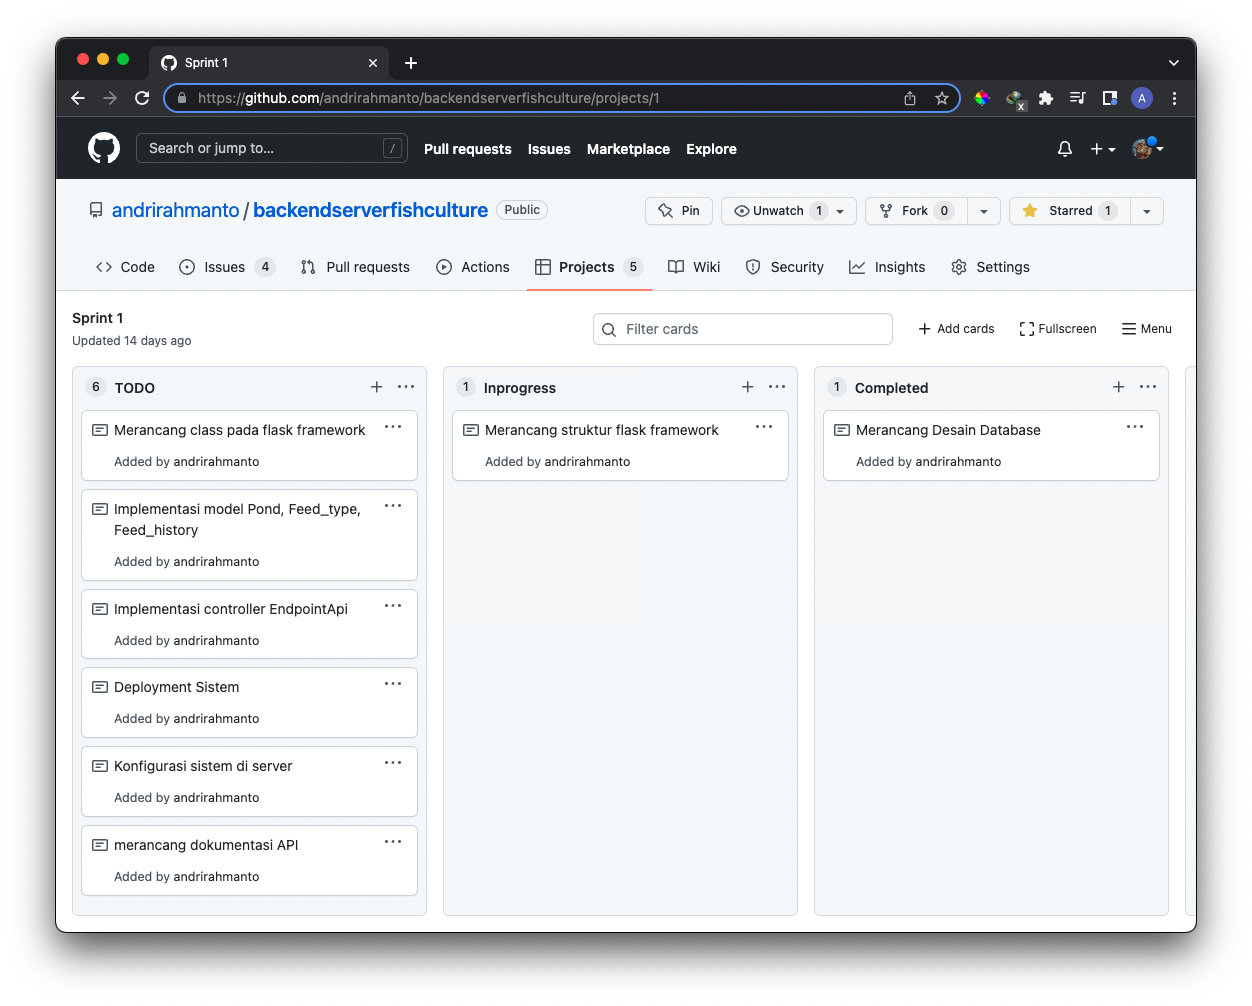
\includegraphics[width=1\textwidth]{gambar/Sprint01/github_project_sprint01.png}
	\caption{Github Projects Sprint-1}
	\label{fig:github_projects_sprint01}
\end{figure}

	Dari \textbf{Gambar \ref{fig:github_projects_sprint01}} diatas, terdapat 4 kolom yang menggambarkan fase dari task tersebut. 4 fase itu adalah to do, in progress, completed, dan tested. To do menandakan fase dimana task baru hanya didaftarkan pada list. In progress menandakan fase dimana task sedang dalam proses pengerjaan oleh developer. Completed merupakan fase dimana task sudah selesai dikerjakan. Dan tested merupakan fase dimana task tertentu telah di test oleh developer dan scrum master.
	
\begin{enumerate}[a).]

	\item{Merancang Database}
	
		Desain Database atau biasa disebut Entity Relationship Diagram (ERD) pada sprint-1 menggambarkan struktur data dan relasi antar data yang akan disimpan pada database. 
	
		\begin{figure}[H]
			\centering
			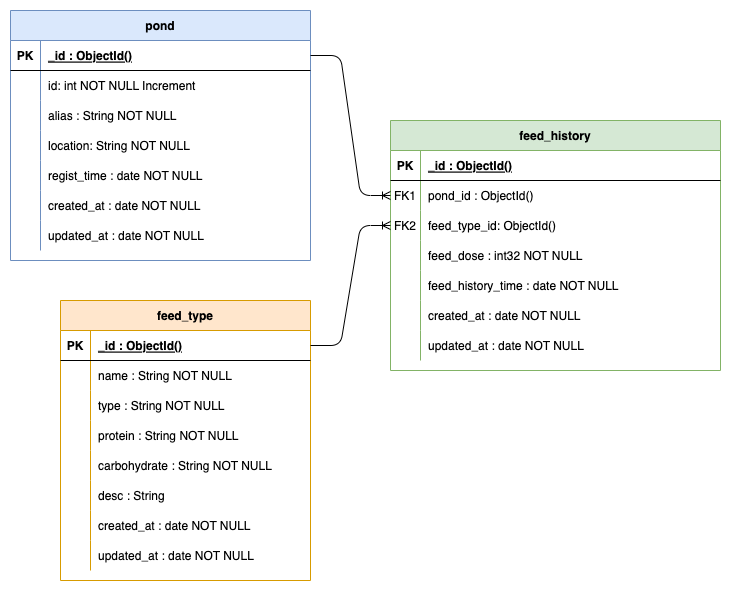
\includegraphics[width=0.7\textwidth]{gambar/Sprint01/diagram database/database.png}
			\caption{ERD Database Sprint-1}
			\label{fig:erd_database_sprint01}
		\end{figure}
		
		Terdapat 3 tabel yang dibutuhkan untuk menunjang fitur pemberian pakan. Tabel pond tabel pond berfungsi untuk menyimpan data terkait kolam, dimana ada beberapa field yaitu nama dan lokasi kolam. Tabel \textit{feed\_type} berfungsi menyimpan data terkait tipe pakan, dimana field yang disimpan adalah nama pakan, tipe pakan, kandungan protein pakan dalam bentuk persentase, kandungan karbohidrat pakan dalam bentuk persentase, dan keterangan tambahan. Tabel \textit{feed\_history} berfungsi untuk menyimpan data terkait pemberian pakan, dimana field yang disimpan adalah id kolam, id tipe pakan, dosis pakan, dan waktu pemberian pakan.
		
	\item{Merancang Struktur Flask Framework}
	
	Rancangan struktur flask framework menggambarkan direktori-direktori pada sistem yang akan di buat. terdapat 4 direktori penting yaitu database, resource, static, template. Direktori database berisi file yang berkaitan dengan database mongodb yaitu, koneksi database dan model data pada database. Direktori resource deskripsi routes dan controller untuk setiap logic API endpoint. Direktori static berisi hal-hal yang dibutuhkan untuk styling sebuah halaman html, yang biasanya berisi css file dan javascript file. Direktori template merupakan tempat penulis menyimpan html file. Pembagian direktori tersebut bertujuan untuk mempermudah pengolahan dalam pengembangan sistem kedepannya.
	
\begin{forest}
  pic dir tree,
  where level=0{}{% folder icons by default; override using file for file icons
    directory,
  },
  [fishapi
    [\_\_init\_\_.py, file]
    [database
    	[\_\_init\_\_.py, file]
	[db.py,file]
	[models.py,file]
    ]
    [index.wsgi, file]
    [resources
      [\_\_init\_\_.py, file]
      [controller
      	  [\_\_init\_\_.py, file]
	  [feed\_history.py,file]
	  [feed\_type.py,file]
	  [pond.py,file]
      ]
      [routes.py,file]
    ]
    [settings.cfg, file]
    [static]
    [templates]
  ]
\end{forest}
		
	\item{Merancang Class Diagram}
	
	Class Diagram menggambarkan kelas-kelas yang akan dipakai oleh sistem. Umumnya terdapat 3 kelas pada setiap module yaitu class model, controller, dan view. Untuk sprint-1 setiap modul hanya terdapat 2 class yaitu model, dan controller.
	
	\begin{figure}[H]
		\centering
		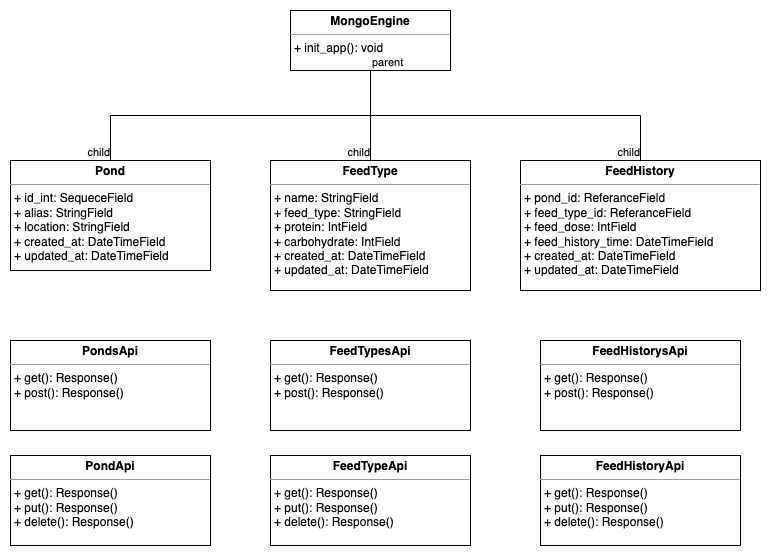
\includegraphics[width=0.9\textwidth]{gambar/Sprint01/class diagram/class_diagram.png}
		\caption{Class Diagram Sprint-1}
		\label{fig:class_diagram_sprint01}
	\end{figure}
	
	Pada \textbf{Gambar \ref{fig:class_diagram_sprint01}} setiap module terdapat 3 class. Semisal module Pond terdapat 1 class untuk model dan 2 class controller API. class model merupakan class yang mewarisi sifat MongoEngine.Document yang merupakan sebuah package pada python untuk mempermudah manipulasi database. Sedangkan class controller API merupakan class yang dibuat untuk mendeskripsikan logic yang akan dijalankan setiap client mengakses API Endpoint.
	
	\item{Implementasi model Pond, Feed\_type, Feed\_history}
	
	Implementasi model dilakukan menggunakan bantuan package Mongoengine yang mana mengharuskan menjadikan Mongoengine.Document sebagai parent dari class tersebut. Pada setiap atribut class harus didefinisikan terhadap jenis field yang telah disediakan oleh Mongoengine.
	
	\begin{enumerate}[1).]
		\item{Model Pond}
			\begin{lstlisting}
class Pond(db.Document):
    id_int = db.SequenceField(required=True)
    alias = db.StringField(required=True)
    location = db.StringField(required=True)
    created_at = db.DateTimeField(default=datetime.datetime.now)
    updated_at = db.DateTimeField(default=datetime.datetime.now)
			\end{lstlisting}
		\item{Model Feed\_type}
			\begin{lstlisting}
class FeedType(db.Document):
    name = db.StringField(required=True)
    feed_type = db.StringField(required=True)
    protein = db.IntField(required=True)
    carbohydrate = db.IntField(required=True)
    desc = db.StringField()
    created_at = db.DateTimeField(default=datetime.datetime.now)
    updated_at = db.DateTimeField(default=datetime.datetime.now)
			\end{lstlisting}
		\item{Model Feed\_history}
			\begin{lstlisting}
class FeedHistory(db.Document):
    pond_id = db.ReferenceField(Pond, required=True)
    feed_type_id = db.ReferenceField(FeedType, required=True)
    feed_dose = db.IntField(required=True)
    feed_history_time = db.DateTimeField(default=datetime.datetime.now)
    created_at = db.DateTimeField(default=datetime.datetime.now)
    updated_at = db.DateTimeField(default=datetime.datetime.now)
    			\end{lstlisting}
	\end{enumerate}
	
	\item{Implementasi Controller EndpointAPI}
	
	\begin{enumerate}[1).]
		\item{Add Routes}
			\begin{lstlisting}
def initialize_routes(api):
    # pond
    api.add_resource(PondsApi, '/api/ponds')
    api.add_resource(PondApi, '/api/ponds/<id>')
			\end{lstlisting}
		\item{PondsApi}
			Class PondsApi
			\begin{lstlisting}
class PondsApi(Resource):
    def get(self):
        objects = Pond.objects()
        response = []
        for pond in objects:
            pond = pond.to_mongo()
            response.append(pond)
        response_dump = json.dumps(response, default=str)
        return Response(response_dump, mimetype="application/json", status=200)

    def post(self):
        body = {
            "alias": request.form.get("alias", None),
            "location": request.form.get("location", None),
        }
        pond = Pond(**body).save()
        id = pond.id
        return {'id': str(id)}, 200
    			\end{lstlisting}
		\item{PondApi}
			\begin{lstlisting}
class PondApi(Resource):
    def put(self, id):
        body = {
            "alias": request.form.get("alias", None),
            "location": request.form.get("location", None),
            "updated_at": datetime.datetime.utcnow()
        }
        Pond.objects.get(id=id).update(**body)
        return '', 200

    def delete(self, id):
        pond = Pond.objects.get(id=id).delete()
        return '', 200

    def get(self, id):
        objects = Pond.objects.get(id=id)
        pond = objects.to_mongo()
        response_dump = json.dumps(pond, default=str)
        return Response(response_dump, mimetype="application/json", status=200)
    			\end{lstlisting}
	\end{enumerate}
	
	\item{Deployment Sistem}
	
	Sistem pada akhirnya dijalankan pada server agar dapat diakses client melalui akses internet. Pertama yang dilakukan adalah mengunggah repositori sistem ke repositori github. Repositori github terdapat pada \textit{\textbf{https://github.com/andrirahmanto/backendserverfishculture/tree/sprint\_01}}. Lalu setelahnya adalah menghubungkan personal computer penulis ke server dengan metode SSH (Secure Shell Connection). Menghubungkan dengan metode ssh dilakukan melalui terminal pada dengan cara
\begin{lstlisting}
ssh <user>@<ip_address_server>
\end{lstlisting}
dan masukan password ketika diminta.

	Selanjutnya hubungkan server dengan repositori github yang sudah dibuat menggunakan metode git remote. 
\begin{lstlisting}
mkdir /var/www/html/<name_your_repo>
git init
git remote add origin <link_github>
git pull origin main
\end{lstlisting}
dengan begitu server telah memiliki repo yang sama dengan yang ada di personal komputer. Langkah selanjutnya diikuti dengan penginstalan package yang dipakai pada sistem.

	\item{Konfigurasi Sistem pada Server}

	Konfigurasi bertujuan untuk menjalankan sistem yang sudah di upload ke server. Tahapan pertama konfigurasi adalah memastikan bahwa sistem berbentuk package agar dapat di import. kemudian buat file index.wsgi seperti dibawah ini
\begin{lstlisting}
import logging
import sys

logging.basicConfig(stream=sys.stderr)
sys.path.insert(0, '/var/www/html/fishapi')

from fishapi import create_app
application = create_app()
\end{lstlisting}
	index.wsgi nantinya akan didaftarkan ke file httpd.conf pada server agar sistem dapat dieksekusi oleh server.
\begin{lstlisting}
WSGIDaemonProcess /fishapi python-path=/opt/rh/rh-python38/root/lib/pyt$
WSGIProcessGroup /fishapi
WSGIApplicationGroup %{GLOBAL}
WSGIScriptAlias /fishapi /var/www/html/fishapi/index.wsgi
WSGIScriptReloading on
<Directory "/var/www/html/fishapi/fishapi">
	AllowOverride All
	Options +ExecCGI
	AddHandler cgi-script .cgi .pl .py
	Order allow,deny
	allow from all
</Directory>

Alias /fishapi/static /var/www/html/fishapi/fishapi/static
<Directory /var/www/html/fishapi/fishapi/static>
	AllowOverride All
	Order allow,deny
	allow from all
</Directory>
\end{lstlisting}
Setelahnya lakukan restart pada apache pada server dengan menjalankan:
\begin{lstlisting}
systemctl restart http
\end{lstlisting}
Setelah konfigurasi selesai, sistem akan di test pada browser dengan melakukan request.
\begin{figure}[H]
		\centering
		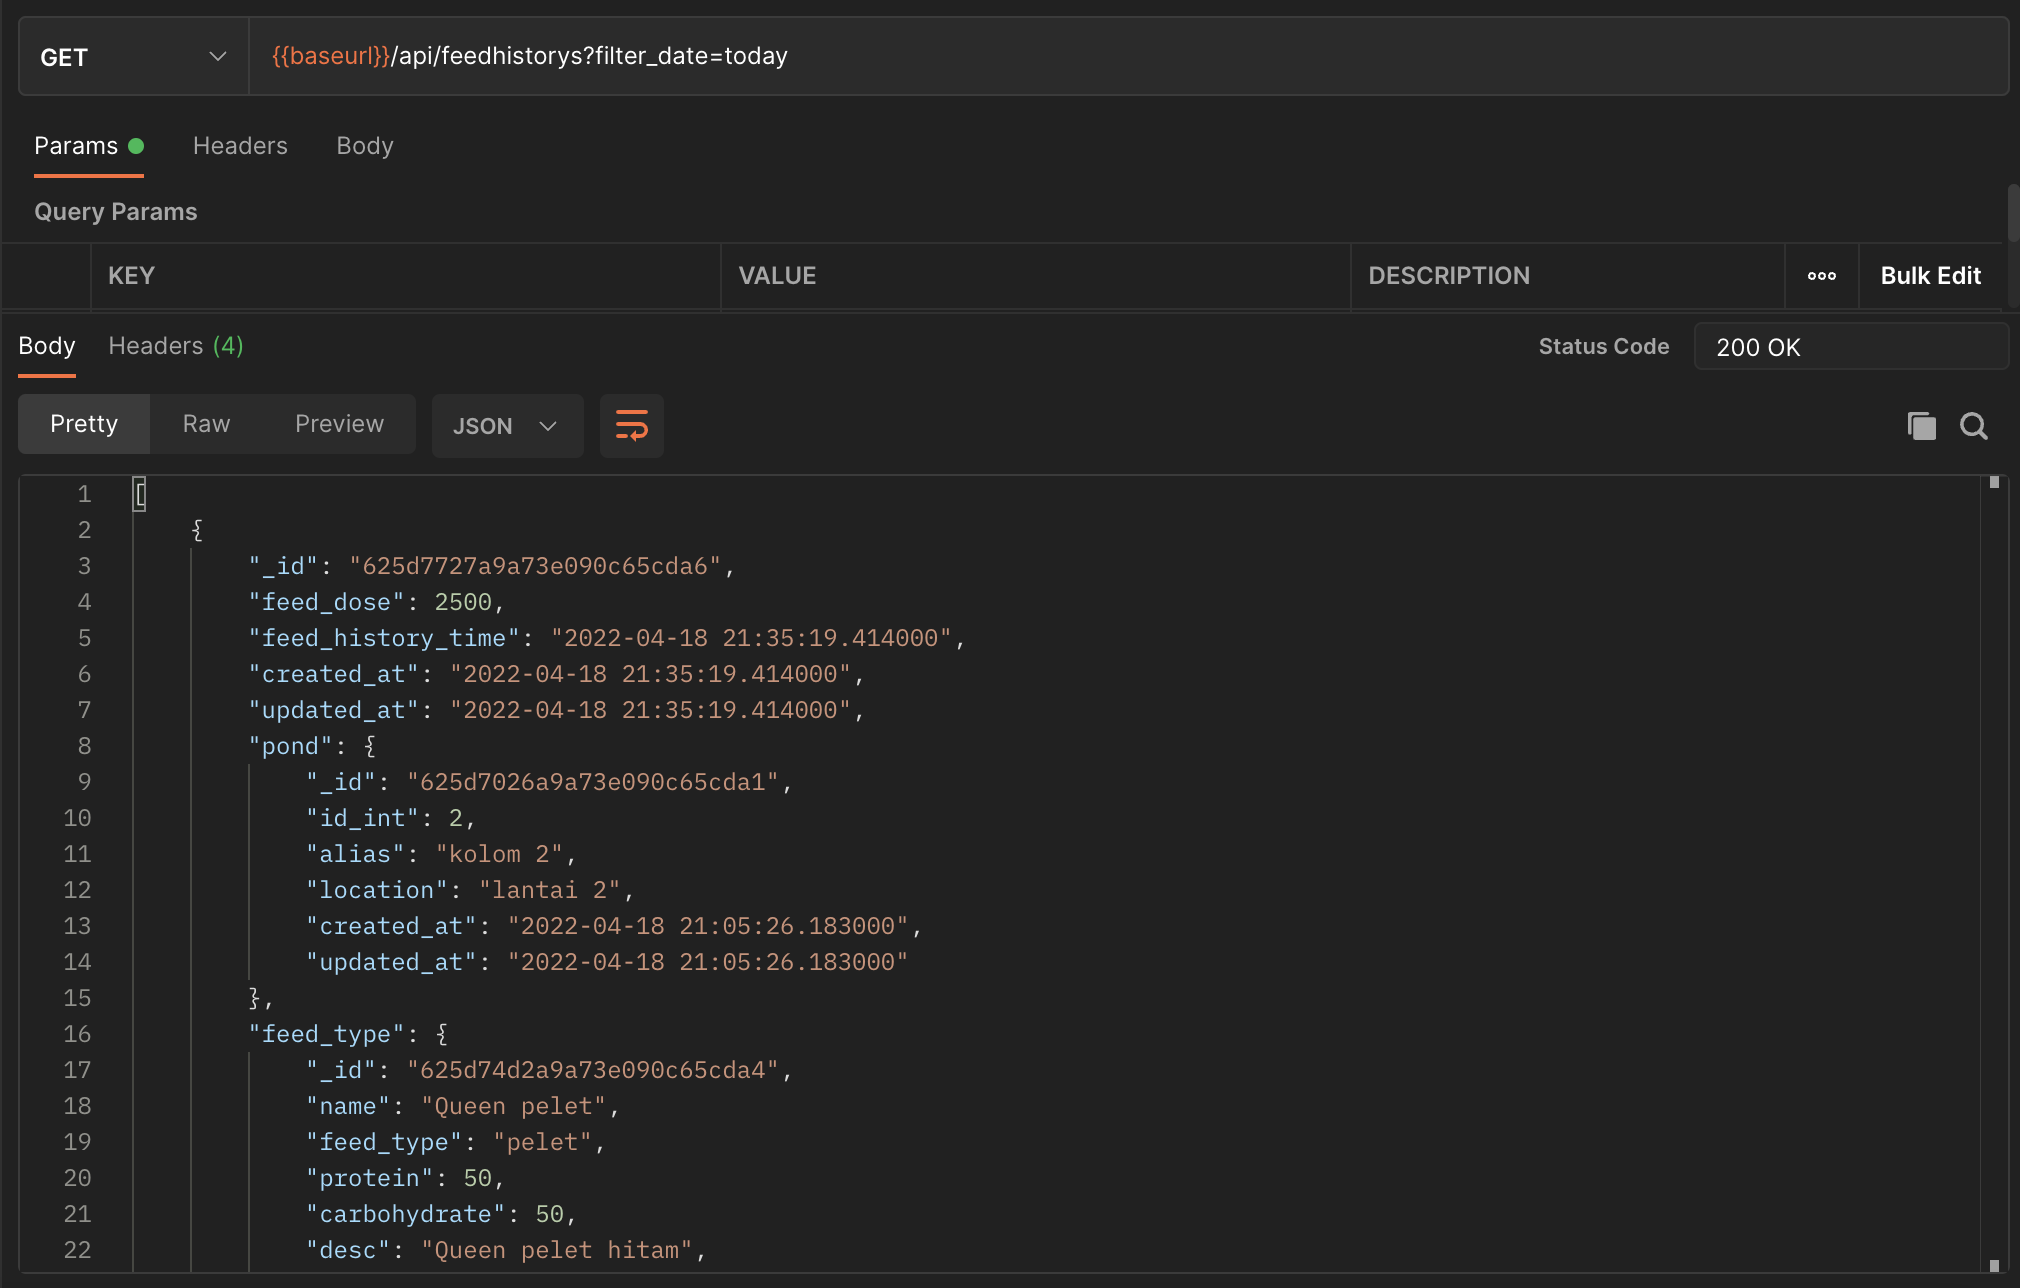
\includegraphics[width=0.9\textwidth]{gambar/Sprint01/request_get.png}
    		\caption{\textit{Request Get \emph{pemberian pakan} Postman}}
		\label{fig:request_get}
\end{figure}
	
	
	\item{Dokumentasi API}
	
	Dokumentasi API dibuat menggunakan postman, yang mana dapat diakses melalui link \textit{\textbf{https://documenter.getpostman.com/view/11714934/UVysybzY}}.
	berikut beberapa contoh request dan response yang diberikan server:
	request cURL:
\begin{lstlisting}
curl --location --request GET 'http://jft.web.id/fishapi/api/ponds'
\end{lstlisting}
	response json:
\begin{lstlisting}
[
  {
    "_id": "625d7026a9a73e090c65cda1",
    "id_int": 2,
    "alias": "alpha",
    "location": "blok 1",
    "shape": "bundar",
    "material": "beton",
    "length": 0,
    "width": 0,
    "diameter": 1.4,
    "height": 1,
    "build_at": "2022-04-18 21:05:26.183000",
    "image_name": "kolam_1655141767.jpeg",
    "area": 1.5399999999999998,
    "image_link": "http://127.0.0.1:5000/api/ponds/image/625d7026a9a73e090c65cda1",
    "volume": 1.5399999999999998
  },
  { "_id": "625d7033a9a73e090c65cda2",.....},
  { "_id": "62a62163e445ffb9c5f746f3",......},
  { "_id": "62a955888911334402ddb3b3",.....},
  {"_id": "62a9a466299f257e382a8295",.....}
]
\end{lstlisting}	

	\item{Unit Testing}
	
	Unit Testing dilakukan pada akhir sprint. Adapun hasil dari unit testing yang telah dilaksanakan dapat dilihat pada tabel di bawah ini:
	
\begin{table}[H]
	\centering
	\caption{Unit Testing Sprint 1}
	\label{table:unittesting_sprint1}
	\begin{tabular}{|l|l|ll|l|}
\hline
\multirow{2}{*}{No} & \multirow{2}{*}{Skenario Pengujian} & \multicolumn{2}{l|}{Kesesuaian}     & \multirow{2}{*}{Kesimpulan} \\ \cline{3-4}
                    &                                     & \multicolumn{1}{l|}{Sesuai} & Tidak &                             \\ \hline
1  & Pencatatan pemberian pakan          & \multicolumn{1}{l|}{\CheckmarkBold}&& Diterima \\\hline
2  & Merubah data pemberian pakan          & \multicolumn{1}{l|}{\CheckmarkBold}&& Diterima \\\hline
3  & Mendapatkan list data pemberian pakan          & \multicolumn{1}{l|}{\CheckmarkBold}&& Diterima \\\hline
4  & Mendapatkan detail data pemberian pakan          & \multicolumn{1}{l|}{\CheckmarkBold}&& Diterima \\\hline
5  & Menghapus data pemberian pakan          & \multicolumn{1}{l|}{\CheckmarkBold}&& Diterima \\\hline
\end{tabular}
\end{table}
\end{enumerate}
%!TEX root = ./template-skripsi.tex

\subsection{Sprint 2 Report}
Berikut merupakan report dari sprint ke-2 yang dilakukan pada tanggal 1 juni -7 juni 2022.

\begin{table}[H]
	\caption{\textit{Sprint-2 backlog}}
	\label{sprint2_backlog}
	\begin{tabular}{@{} |p{0.5cm}|p{5cm}|p{5cm}|p{2cm}| @{}}
		\hline
		\textbf{No} & \textbf{\textit{Story}} & \textbf{\textit{Task}} & \textbf{\textit{Status}} \\
		\hline
		1 & \multirow{3}{5cm}{Create, Read, Updte, dan Delete untuk Pencatatan Pemberian pakan} & Membuat view pakan bulanan & Completed\\
		\cline{1-1}\cline{3-4}
		2 & & Membuat view pakan harian & Completed\\
		\cline{1-1}\cline{3-4}
		\hline
	\end{tabular}
\end{table}

\begin{enumerate}[1.]
\item View pakan bulanan
\begin{figure}[H]
	\centering
	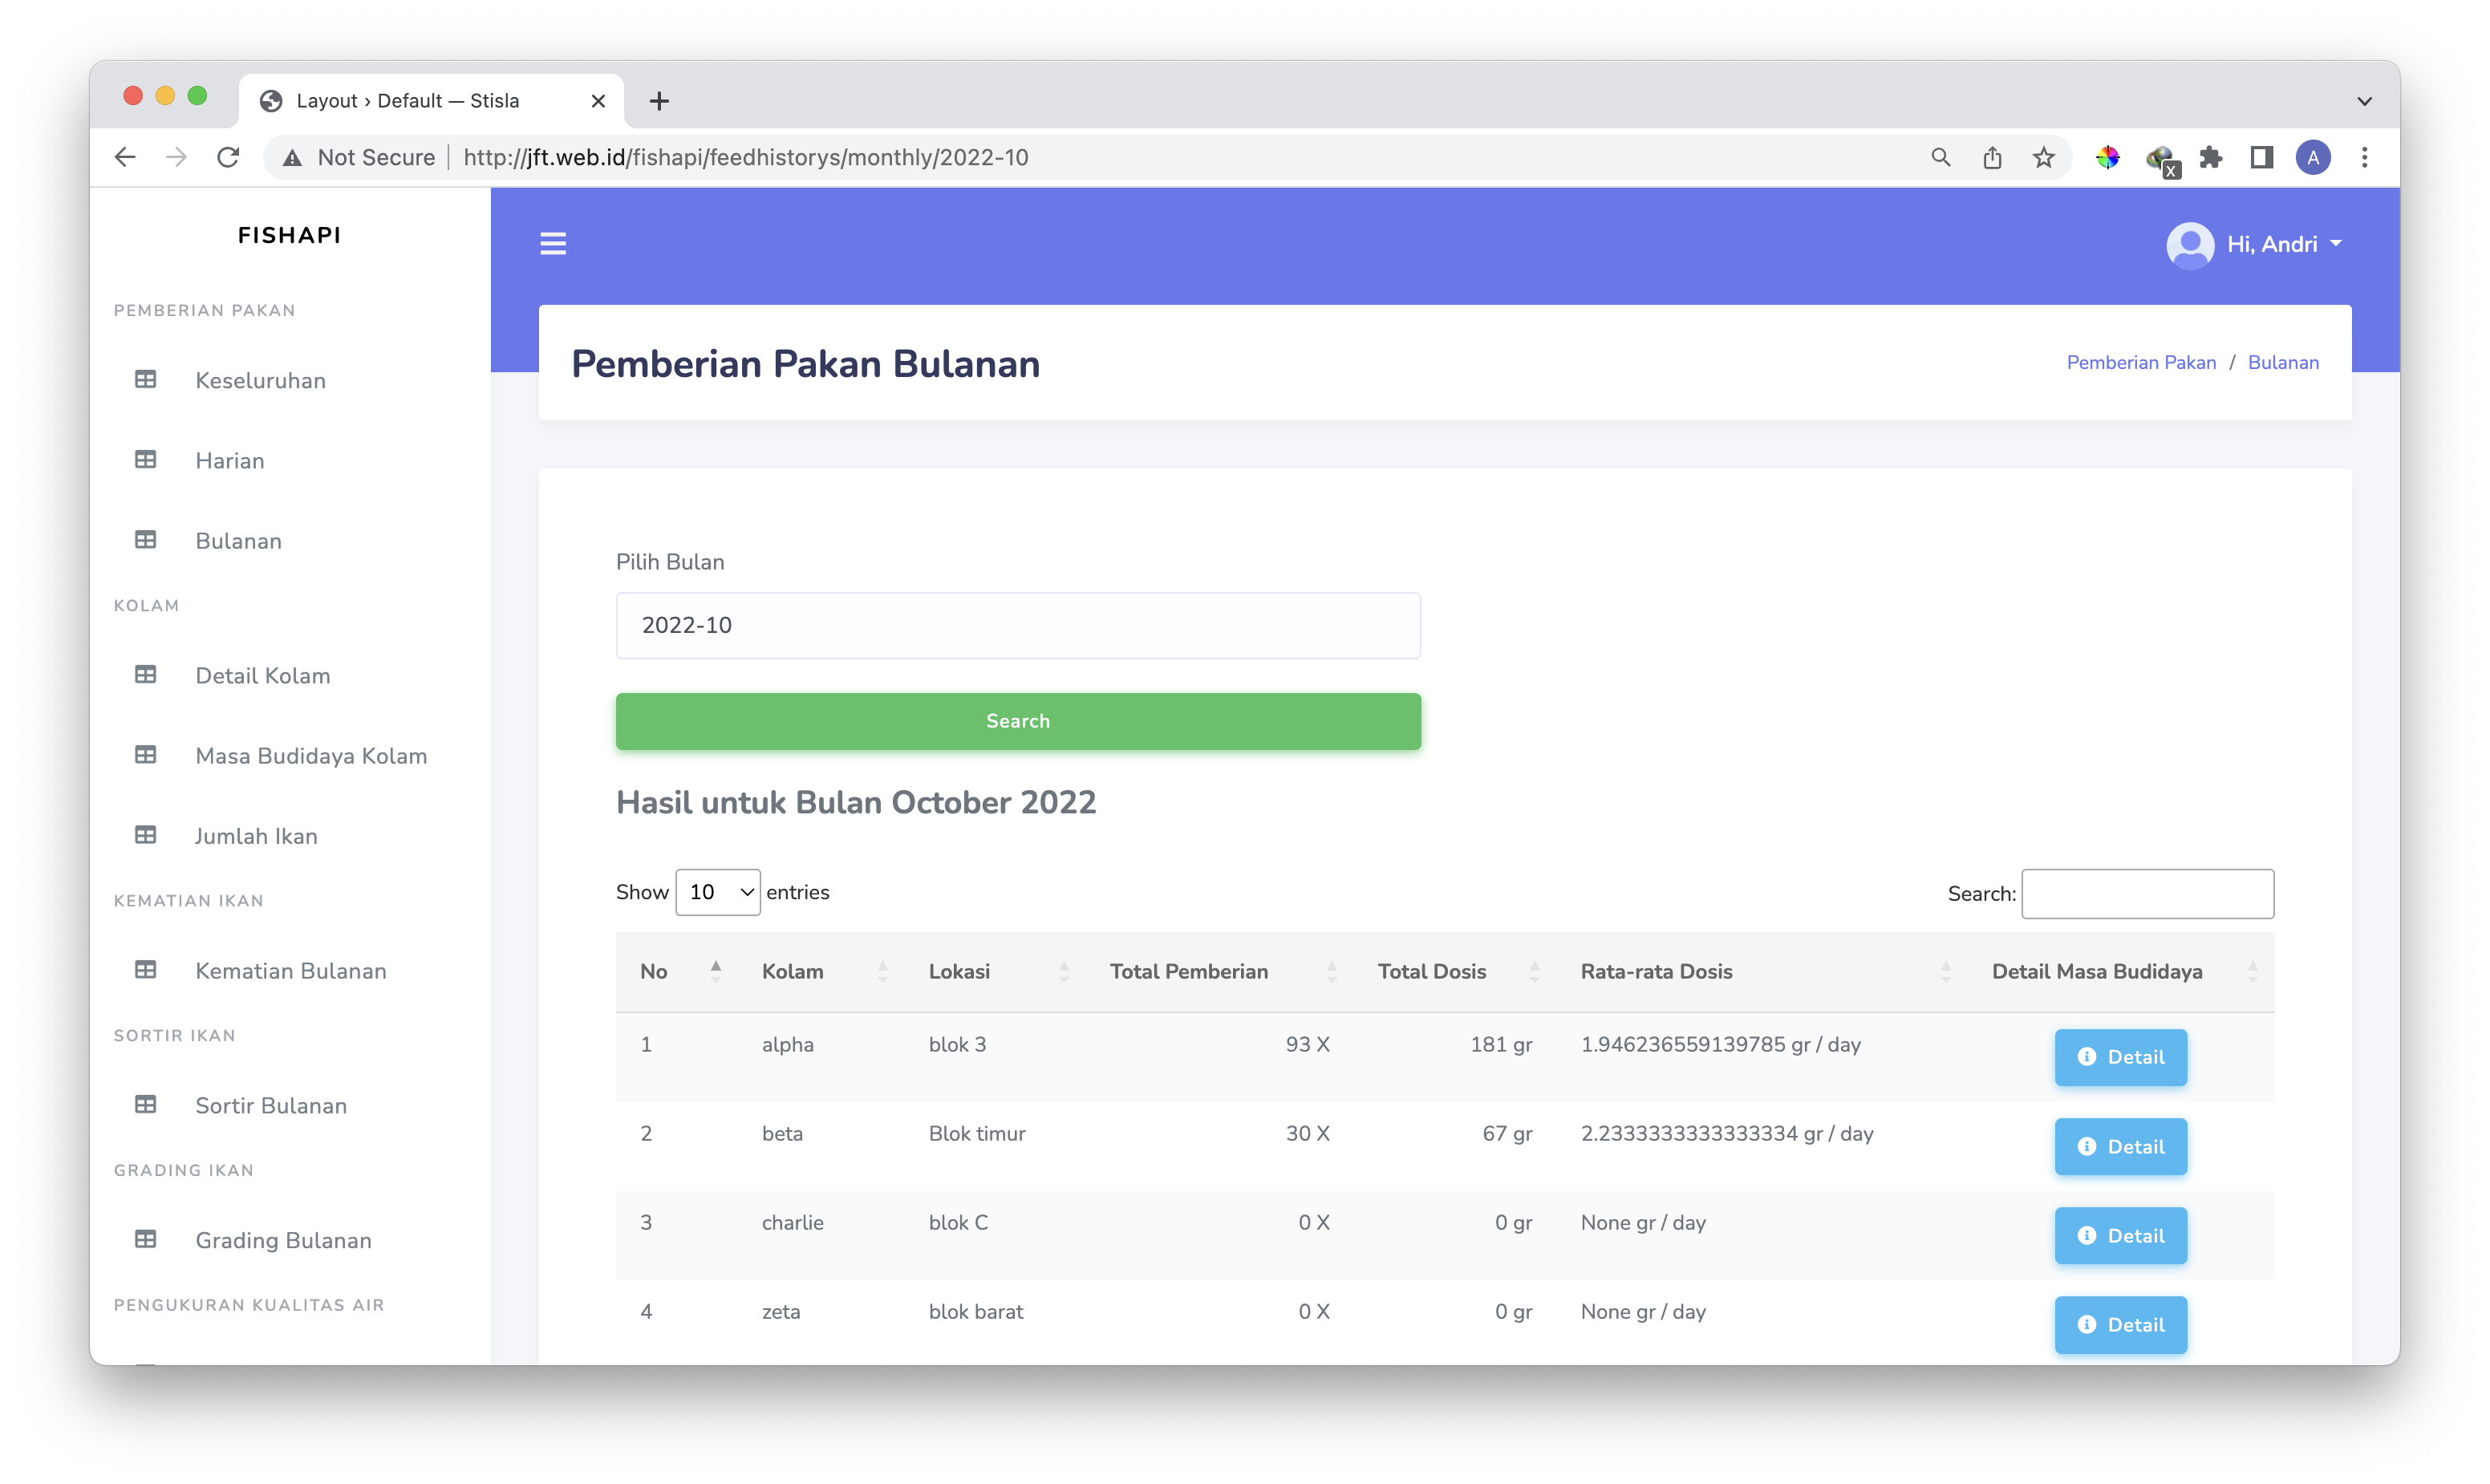
\includegraphics[width=1\textwidth]{gambar/Sprint02/view_pakan_bulanan}
	\caption{View pakan bulanan}
	\label{fig:view_pakan_bulanan}
\end{figure}
	
\item View pakan harian
\begin{figure}[H]
	\centering
	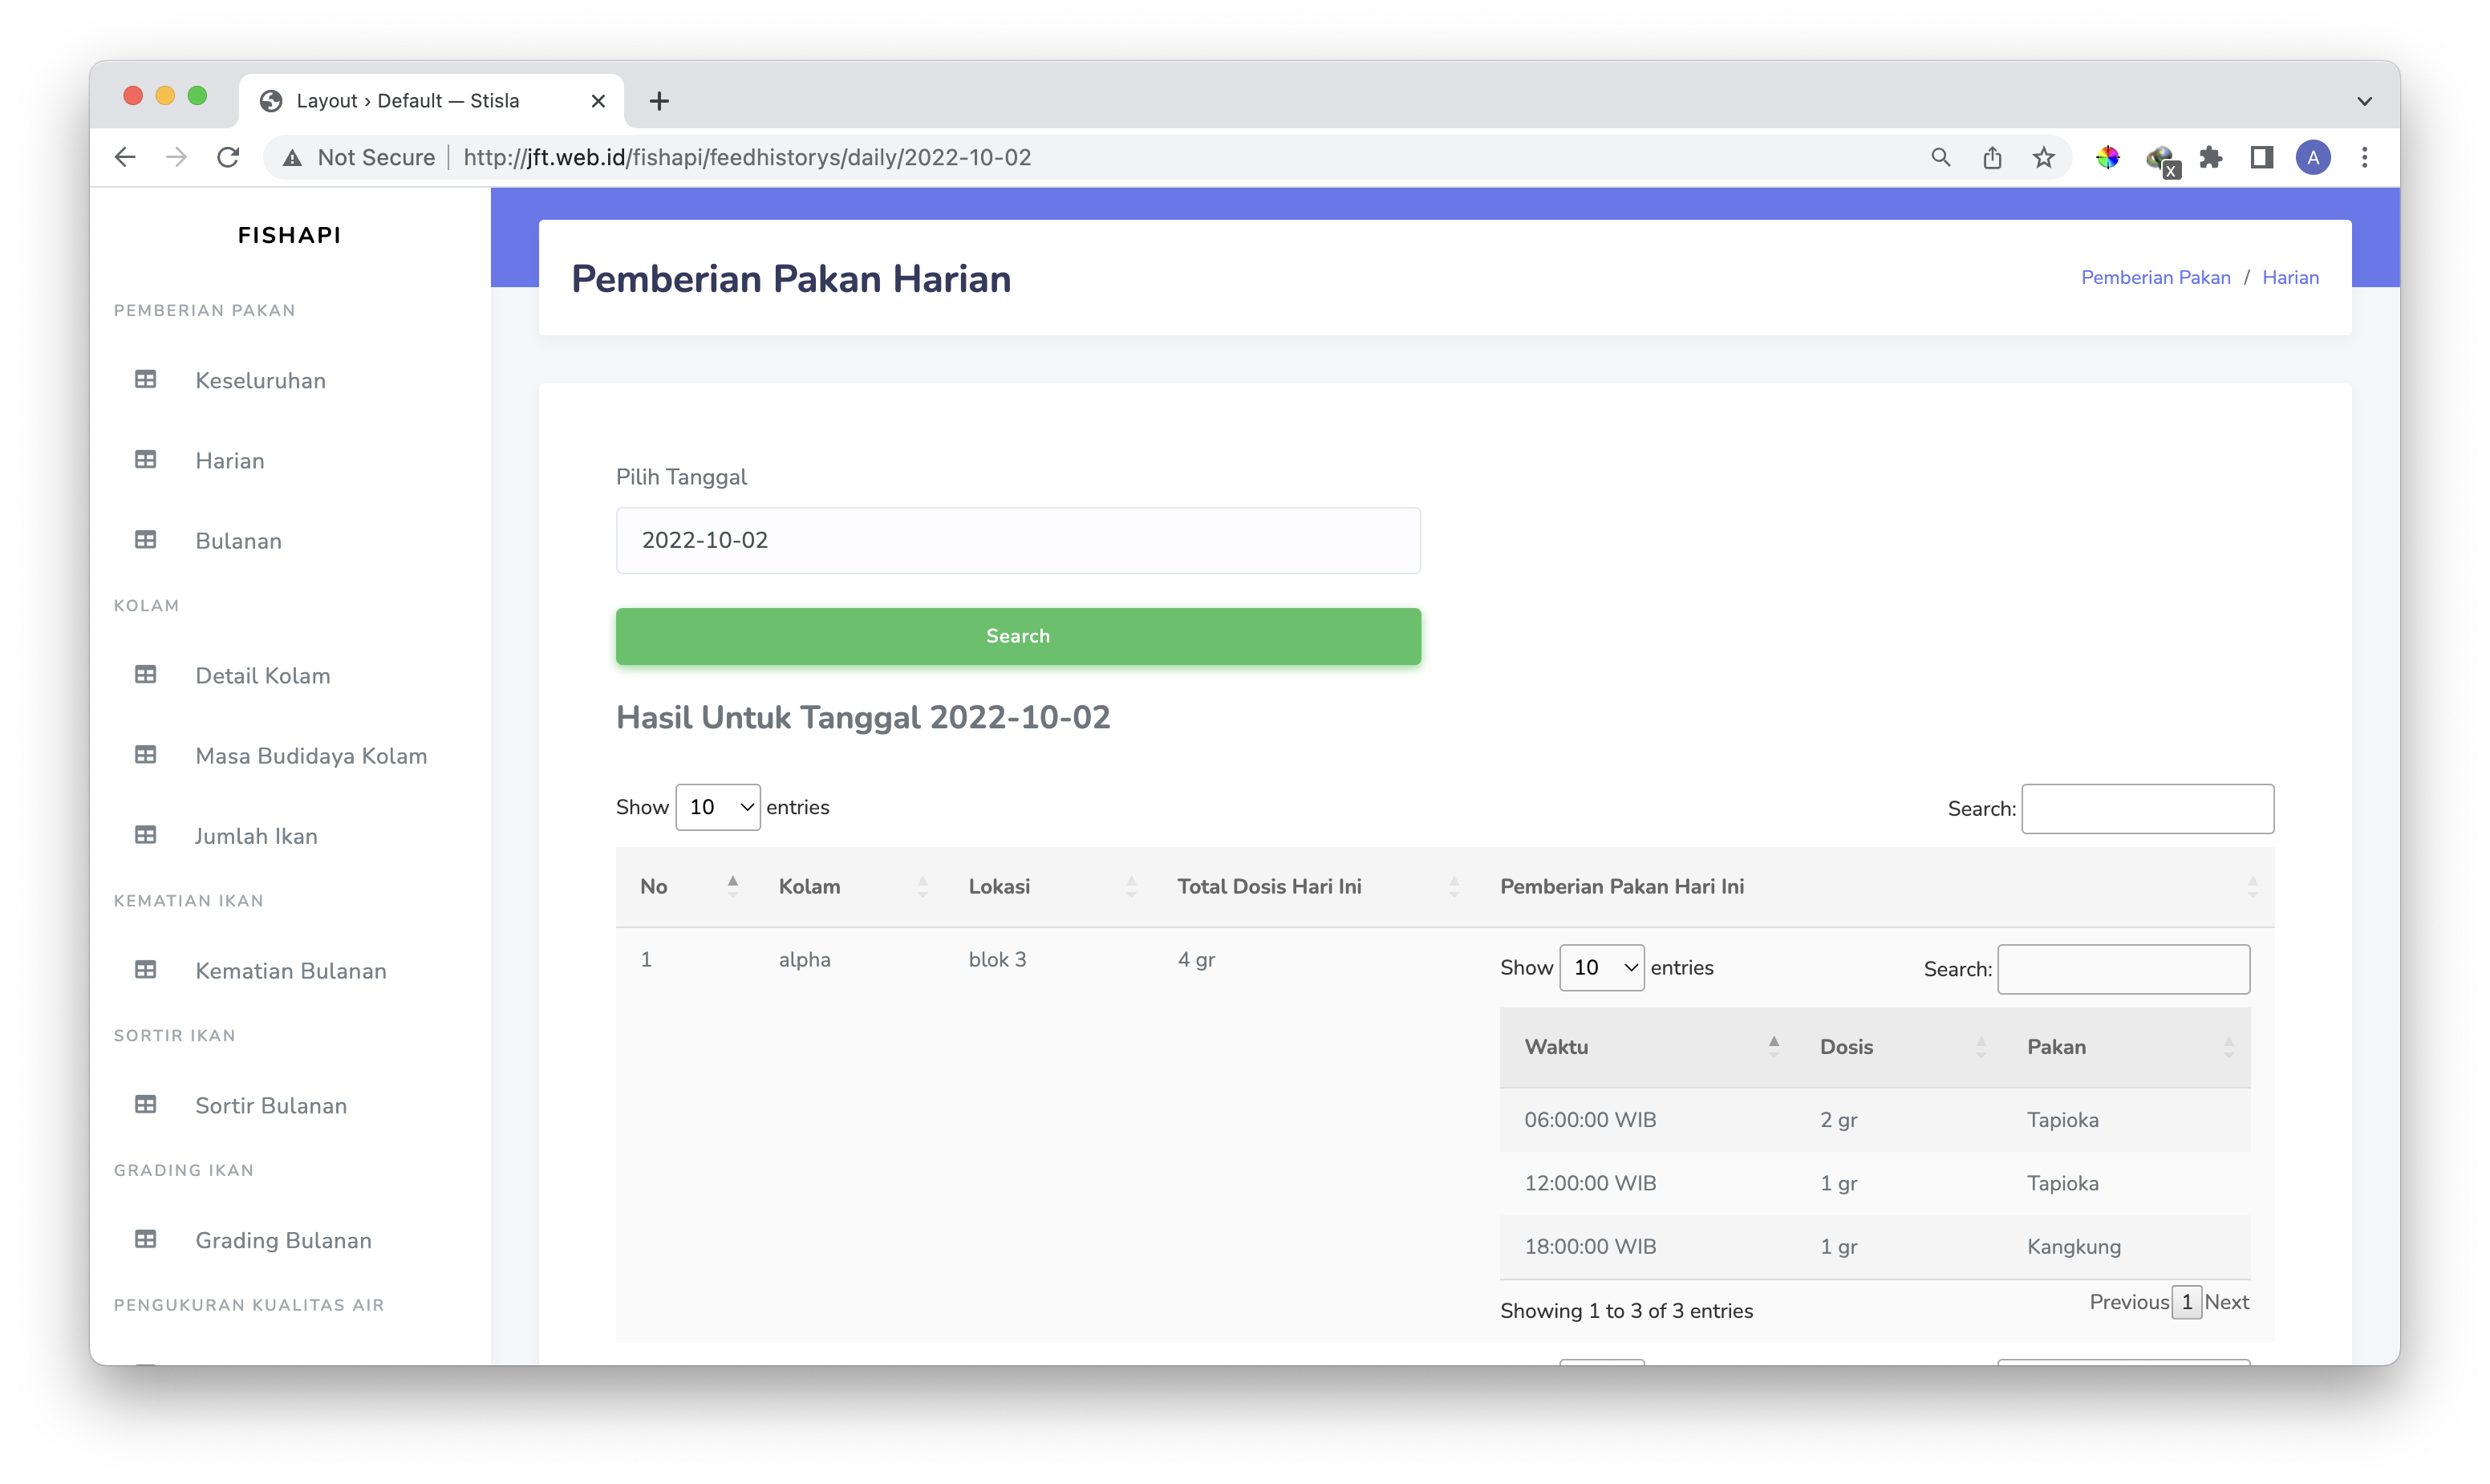
\includegraphics[width=1\textwidth]{gambar/Sprint02/view_pakan_harian}
	\caption{View pakan harian}
	\label{fig:view_pakan_harian}
\end{figure}
\end{enumerate}
%!TEX root = ./template-skripsi.tex

\subsection{Sprint 3 Report}
Berikut merupakan report dari sprint ke-3 yang dilakukan pada tanggal 8 juni - 14 juni 2022.

\begin{table}[H]
	\caption{\textit{Sprint-3 backlog}}
	\label{sprint3_backlog}
	\begin{tabular}{@{} |p{0.5cm}|p{5cm}|p{5cm}|p{2cm}| @{}}
		\hline
		\textbf{No} & \textbf{\textit{Story}} & \textbf{\textit{Task}} & \textbf{\textit{Status}} \\
		\hline
		1 & \multirow{3}{5cm}{Create, Read, Updte, dan Delete untuk Registrasi kolam} & Membarui desain database  & Completed\\
		\cline{1-1}\cline{3-4}
		2 & & Membarui API entry kolam & Completed\\
		\cline{1-1}\cline{3-4}
		3 & & Membarui API edit kolam & Completed\\
		\cline{1-1}\cline{3-4}
		4 & & Membarui API fetch list kolam & Completed\\
		\cline{1-1}\cline{3-4}
		5 & & Membuat API edit foto kolam & Completed\\
		\cline{1-1}\cline{3-4}
		6 & & Membuat API fetch foto kolam & Completed\\
		\cline{1-1}\cline{3-4}
		7 & & Membuat View detail kolam & Completed\\
		\cline{1-1}\cline{3-4}
		\hline
	\end{tabular}
\end{table}

\begin{enumerate}[1.]

\item Desain database
\begin{figure}[H]
	\centering
	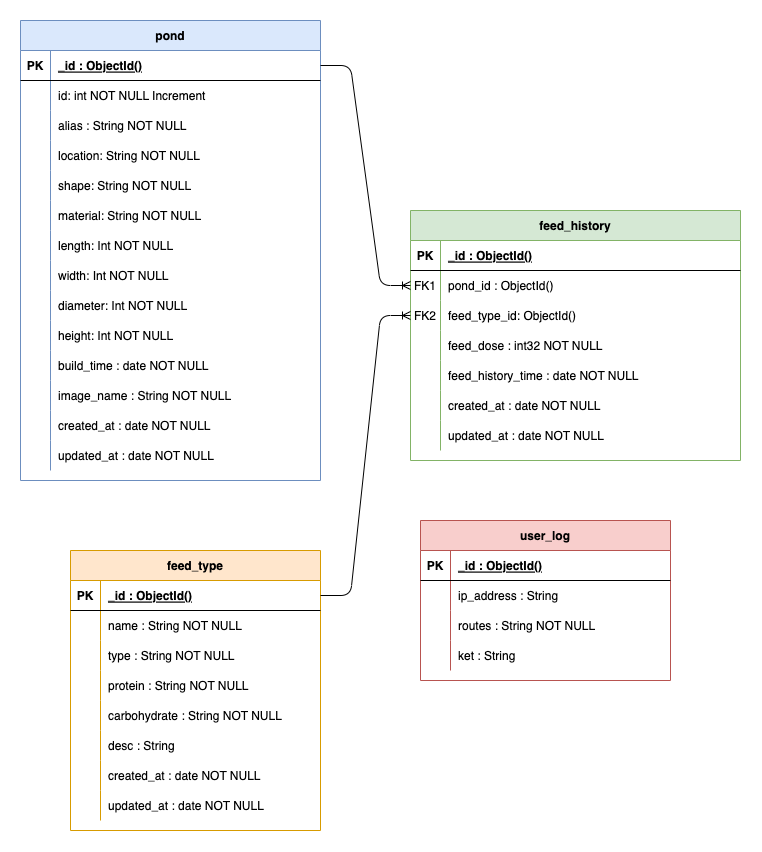
\includegraphics[height=0.7\textwidth]{gambar/Sprint03/diagram database/database}
	\caption{ERD Database Sprint-3}
	\label{fig:database_sprint3}
\end{figure}

Dengan berubahnya desain database diperlukan juga perubahan model pada source code, berikut perubahan pada source code model kolam.

\begin{lstlisting}
# fishapi/database/model.py

class Pond(db.Document):
    id_int = db.SequenceField(required=True)
    alias = db.StringField(required=True)
    location = db.StringField(required=True)
    shape = db.StringField(required=True)
    material = db.StringField(required=True)
    length = db.FloatField(required=True, default=0)
    width = db.FloatField(required=True, default=0)
    diameter = db.FloatField(required=True, default=0)
    height = db.FloatField(required=True, default=0)
    image_name = db.StringField(required=True, default='default.jpg')
    build_at = db.DateTimeField(default=datetime.datetime.now)
    created_at = db.DateTimeField(default=datetime.datetime.now)
    updated_at = db.DateTimeField(default=datetime.datetime.now)
\end{lstlisting}

\item Membarui API entry kolam

Perubahan terjadi pada controller API entry kolam, berikut merupakan perubahan source code controller API entry kolam.
\begin{lstlisting}
# fishapi/resources/controller/pond.py

def post(self):
        try:
            body = {
                "alias": request.form.get("alias", None),
                "location": request.form.get("location", None),
                "shape": request.form.get("shape", None),
                "material": request.form.get("material", None),
                "length": request.form.get("length", None),
                "width": request.form.get("width", None),
                "diameter": request.form.get("diameter", None),
                "height": request.form.get("height", None),
                "build_at": request.form.get("build_at", None),
            }
            pond = Pond(**body).save()
            id = pond.id
            response = {"message": "success add pond", "id": id}
            response = json.dumps(response, default=str)
            return Response(response, mimetype="application/json", status=200)
        except Exception as e:
            response = {"message": str(e)}
            response = json.dumps(response, default=str)
            return Response(response, mimetype="application/json", status=400)
\end{lstlisting}

Fungsi ini merupakan sebuah endpoint HTTP POST yang digunakan untuk menambahkan data kolam ke dalam database.

Pada bagian awal fungsi, request.form.get digunakan untuk membaca nilai dari setiap parameter dari request yang dikirim melalui form-data. Nilai-nilai ini kemudian digabungkan menjadi satu objek body.

Kemudian, objek Pond yang baru dibuat dengan parameter yang diambil dari objek body tersebut. Setelah itu, fungsi "save()" digunakan untuk menyimpan objek Pond ke dalam database.

Jika operasi penyimpanan berhasil dilakukan, fungsi akan memberikan respons dengan status kode 200 dan pesan "success add pond" beserta ID dari kolam yang baru saja ditambahkan. Jika terjadi kesalahan dalam proses ini, fungsi akan memberikan respons dengan status kode 400 dan pesan kesalahan dalam format JSON.

Fungsi json.dumps() digunakan untuk mengkonversi objek response ke dalam format JSON dan menentukan parameter default=str agar objek dapat di-serialize dalam format JSON. Terakhir, fungsi mengembalikan respons dengan header "application/json".

Berikut merupakan form untuk entry kolam.

% Please add the following required packages to your document preamble:
% \usepackage[table,xcdraw]{xcolor}
% If you use beamer only pass "xcolor=table" option, i.e. \documentclass[xcolor=table]{beamer}
\begin{table}[]
\begin{tabular}{|l|l|l|}
\hline
\multicolumn{1}{|c|}{\cellcolor[HTML]{F9F9F9}\textbf{Form}} & \multicolumn{1}{c|}{\cellcolor[HTML]{F9F9F9}\textbf{Jenis}}                                                               & \textbf{Deskripsi}     \\ \hline
{\color[HTML]{212121} alias}                                & {\color[HTML]{212121} REQUIRED STRING}                                                                                    & alias/nama untuk kolam \\ \hline
{\color[HTML]{212121} location}                             & {\color[HTML]{212121} REQUIRED STRING}                                                                                    & lokasi kolam           \\ \hline
{\color[HTML]{212121} shape}                                & {\color[HTML]{212121} \begin{tabular}[c]{@{}l@{}}REQUIRED STRING\\ VALUE : {[}'persegi', 'bundar'{]}\end{tabular}}        & bentuk kolam           \\ \hline
{\color[HTML]{212121} material}                             & {\color[HTML]{212121} \begin{tabular}[c]{@{}l@{}}REQUIRED STRING\\ VALUE : {[}'tanah', 'terpal', 'beton'{]}\end{tabular}} & bahan bangun kolam     \\ \hline
{\color[HTML]{212121} length}                               & {\color[HTML]{212121} REQUIRED DOUBLE FOR SHAPE ('peresgi')}                                                              & panjang kolam          \\ \hline
{\color[HTML]{212121} width}                                & {\color[HTML]{212121} REQUIRED DOUBLE FOR SHAPE ('peresgi')}                                                              & lebar kolam            \\ \hline
{\color[HTML]{212121} diameter}                             & {\color[HTML]{212121} REQUIRED DOUBLE FOR SHAPE ('bundar')}                                                               & diameter kolam         \\ \hline
{\color[HTML]{212121} height}                               & {\color[HTML]{212121} REQUIRED DOUBLE}                                                                                    & tinggi kolam           \\ \hline
{\color[HTML]{212121} build\_at}                            & {\color[HTML]{212121} \begin{tabular}[c]{@{}l@{}}OPTIONAL STRING\\ DATETIME \{YYYY-mm-dd THH:MM:ss\}\end{tabular}}        & tanggal kolam dibuat   \\ \hline
\end{tabular}
\end{table}

Tabel tersebut menjelaskan parameter-parameter yang dibutuhkan untuk membuat suatu kolam dalam suatu program atau sistem. Setiap baris di tabel tersebut menjelaskan satu parameter yang diperlukan untuk membuat kolam, yang terdiri dari tiga kolom:

\begin{enumerate}[a.]
\item Form: kolom ini menjelaskan nama parameter yang dibutuhkan untuk membuat kolam
\item Jenis: kolom ini menjelaskan jenis data yang diperlukan untuk nilai parameter tersebut, termasuk apakah data tersebut wajib atau opsional, dan jika wajib, tipe data apa yang harus digunakan.
\item Deskripsi: kolom ini memberikan deskripsi singkat tentang arti parameter tersebut.
\end{enumerate}

Dalam tabel tersebut, terdapat sembilan parameter yang dibutuhkan untuk membuat kolam, yaitu "alias", "location", "shape", "material", "length", "width", "diameter", "height", dan "build\_at". Beberapa parameter adalah wajib, seperti "alias", "location", "shape", "material", dan "height", sedangkan beberapa parameter lainnya adalah opsional, seperti "build\_at". Terdapat juga beberapa parameter yang memerlukan jenis data khusus, seperti "shape" yang harus bernilai "persegi" atau "bundar", dan "build\_at" yang harus merupakan datetime dalam format tertentu.

Berikut merupakan hasil test request dari API entry kolam.

cURL:

\begin{lstlisting}
curl --location 'http://jft.web.id/fishapi/api/ponds' \
--form 'alias="epsilon"' \
--form 'location="blok 3"' \
--form 'shape="persegi"' \
--form 'material="tanah"' \
--form 'length="5"' \
--form 'width="3"' \
--form 'height="0.7"'
\end{lstlisting}

response json:

\begin{lstlisting}
{
  "message": "success add pond",
  "id": "62aa118fa95cbcb494c5a4a6"
}\end{lstlisting}

\item Membarui API edit kolam

Perubahan terjadi pada controller API edit kolam, berikut merupakan perubahan source code controller API edit kolam.

\begin{lstlisting}
# fishapi/resources/controller/pond.py

def put(self, id):
        try:
            body = request.form.to_dict(flat=True)
            Pond.objects.get(id=id).update(**body)
            response = {"message": "success change data pond", "id": id}
            response = json.dumps(response, default=str)
            return Response(response, mimetype="application/json", status=200)
        except Exception as e:
            response = {"message": str(e)}
            response = json.dumps(response, default=str)
            return Response(response, mimetype="application/json", status=400)
        return
\end{lstlisting}

Fungsi ini merupakan sebuah endpoint HTTP PUT yang digunakan untuk mengubah data kolam yang sudah ada di dalam database.

Saat endpoint ini dipanggil, fungsi akan membaca input yang diberikan melalui form-data dan membuat objek body dengan nilai-nilai parameter tersebut.

Kemudian, fungsi "update()" pada objek Pond yang memiliki ID yang sesuai akan dipanggil dengan parameter nilai-nilai dari objek body tersebut. Fungsi ini akan mengubah nilai dari setiap parameter yang terkait dengan ID kolam tersebut di dalam database.

Jika operasi pengubahan berhasil dilakukan, fungsi akan memberikan respons dengan status kode 200 dan pesan "success change data pond" beserta ID dari kolam yang diubah. Jika terjadi kesalahan dalam proses ini, fungsi akan memberikan respons dengan status kode 400 dan pesan kesalahan dalam format JSON.

Fungsi json.dumps() digunakan untuk mengkonversi objek response ke dalam format JSON dan menentukan parameter default=str agar objek dapat di-serialize dalam format JSON. Terakhir, fungsi mengembalikan respons dengan header "application/json".

Berikut merupakan hasil test request yang dari API edit kolam.

cURL:

\begin{lstlisting}
curl --location -g --request PUT 'http://jft.web.id/fishapi/api/ponds/{pond_id}' \
--form 'material="terpal"'
\end{lstlisting}

response json:

\begin{lstlisting}
{
  "message": "success change data pond",
  "id": "625d7033a9a73e090c65cda2"
}
\end{lstlisting}

\item Membarui API fetch list kolam

Perubahan terjadi pada controller API fetch list kolam, berikut merupakan perubahan source code controller API fetch list kolam.

\begin{lstlisting}
# fishapi/resources/controller/pond.py

def get(self):
        try:
            url = url_for('pondimageapidummy', _external=True)
            pipeline = [
                {"$addFields": {
                    "area": {"$cond": {
                        "if": {"$eq": ["$shape", "persegi"]},
                        "then": {"$multiply": ["$length", "$width"]},
                        "else": {"$divide": [
                            {"$multiply": [22, "$diameter", "$diameter"]},
                            28
                        ]},
                    }},
                    "image_link":{"$concat": [url, "/", {"$toString": "$_id"}]}
                }},
                {"$addFields": {
                    "volume": {"$multiply": ["$area", "$height"]}
                }},
                {"$project": {
                    "pond_id": 0,
                    "feed_type_id": 0,
                    "created_at": 0,
                    "updated_at": 0,
                }}
            ]
            ponds = Pond.objects.aggregate(pipeline)
            list_ponds = list(ponds)
            response = json.dumps(list_ponds, default=str)
            return Response(response, mimetype="application/json", status=200)
        except Exception as e:
            response = {"message": str(e)}
            response = json.dumps(response, default=str)
            return Response(response, mimetype="application/json", status=400)\end{lstlisting}
            
Fungsi ini merupakan sebuah endpoint HTTP GET yang digunakan untuk mengambil data kolam yang sudah ada di dalam database.

Saat endpoint ini dipanggil, fungsi akan melakukan query terhadap database untuk mengambil data kolam yang sudah ada. Query ini dilakukan dengan menggunakan objek pipeline yang akan menambahkan field "area" dan "image\_link" pada hasil query.

Field "area" akan diisi dengan nilai luas kolam yang dihitung berdasarkan shape, length, width, dan diameter kolam. Field "image\_link" akan diisi dengan URL gambar kolam yang diambil dari endpoint "pondimageapidummy".

Setelah itu, field "volume" akan ditambahkan ke hasil query dengan menghitung nilai volume kolam berdasarkan field "area" dan "height".

Terakhir, hasil query akan diproyeksikan ke dalam objek yang hanya mengandung field-field tertentu saja seperti "alias", "location", "shape", "material", "length", "width", "diameter", "height", "area", "volume", dan "image\_link".

Jika query berhasil dilakukan, fungsi akan memberikan respons dengan status kode 200 dan daftar kolam dalam format JSON. Jika terjadi kesalahan dalam proses ini, fungsi akan memberikan respons dengan status kode 400 dan pesan kesalahan dalam format JSON.

Berikut merupakan hasil test request yang dari API fetch list kolam.

cURL:

\begin{lstlisting}
curl --location 'http://jft.web.id/fishapi/api/ponds'
\end{lstlisting}

response json:

\begin{lstlisting}
[
  {
    "_id": "625d7026a9a73e090c65cda1",
    "id_int": 2,
    "alias": "alpha",
    "location": "blok 1",
    "shape": "bundar",
    "material": "beton",
    "length": 0,
    "width": 0,
    "diameter": 1.4,
    "height": 1,
    "build_at": "2022-04-18 21:05:26.183000",
    "image_name": "kolam_1655141767.jpeg",
    "area": 1.5399999999999998,
    "image_link": "http://127.0.0.1:5000/api/ponds/image/625d7026a9a73e090c65cda1",
    "volume": 1.5399999999999998
  },
  {
    "_id": "625d7033a9a73e090c65cda2",
    "id_int": 3,
    "alias": "beta",
    "location": "blok 1",
    "shape": "persegi",
    "material": "terpal",
    "length": 8,
    "width": 4,
    "diameter": 0,
    "height": 1,
    "build_at": "2022-04-18 21:05:39.608000",
    "image_name": "default.jpg",
    "area": 32,
    "image_link": "http://127.0.0.1:5000/api/ponds/image/625d7033a9a73e090c65cda2",
    "volume": 32
  },
  {......
]
\end{lstlisting}

\item Menambahkan API edit foto kolam

Penambahan API untuk fungsi edit foto kolam, berikut merupakan penambahan source code controller API edit foto kolam.

\begin{lstlisting}
# fishapi/resources/controller/pond.py

def put(self, id):
        try:
            file = request.files['image']
            if not file:
                response = {"message": "no file selected"}
                response = json.dumps(response, default=str)
                return Response(response, mimetype="application/json", status=400)
            if not allowed_file(file.filename):
                response = {"message": "file type not allowed"}
                response = json.dumps(response, default=str)
                return Response(response, mimetype="application/json", status=400)
            filename = secure_filename(file.filename)
            filename = pad_timestamp(filename)
            path = os.path.join(current_app.instance_path,
                                current_app.config['UPLOAD_DIR'])
            try:
                os.makedirs(path)
            except OSError:
                pass
            filepath = os.path.join(path, filename)
            file.save(filepath)
            # database
            objects = Pond.objects.get(id=id)
            pond = objects.to_mongo()
            old_image_name = pond["image_name"]
            new_image_name = filename
            if old_image_name != "default.jpg":
                os.remove(os.path.join(path, old_image_name))
            data = {
                "image_name": new_image_name
            }
            objects.update(**data)
            id = objects.id
            response = {"message": "success change image", "id": id}
            response = json.dumps(response, default=str)
            return Response(response, mimetype="application/json", status=200)
        except Exception as e:
            response = {"message": str(e)}
            response = json.dumps(response, default=str)
            return Response(response, mimetype="application/json", status=400)
\end{lstlisting}

Kode tersebut merupakan implementasi dari method PUT pada API untuk mengganti gambar kolam ikan berdasarkan ID kolam. Pertama, API akan menerima request PUT yang berisi file gambar yang ingin diganti dan ID kolam yang ingin diubah gambarnya. Jika tidak ada file gambar yang dipilih, maka akan mengembalikan response "no file selected" dengan status code 400. Jika file yang dipilih tidak diperbolehkan, maka akan mengembalikan response "file type not allowed" dengan status code 400.

Selanjutnya, filename dari file gambar tersebut akan diproses dengan fungsi secure\_filename dan pad\_timestamp untuk memastikan nama file yang aman dan unik. Path untuk menyimpan file gambar akan dibuat, dan file akan disimpan di path tersebut.

Kemudian, API akan mengambil data kolam ikan berdasarkan ID yang diberikan dari database. Gambar lama dari kolam ikan tersebut akan dihapus jika bukan "default.jpg" dan digantikan dengan gambar baru yang telah dipilih.

Terakhir, API akan mengembalikan response "success change image" beserta ID kolam ikan yang diubah gambarnya dengan status code 200. Jika terjadi error pada proses ini, maka akan mengembalikan response dengan pesan error dan status code 400.

Berikut merupakan hasil test request yang dari API edit foto kolam. Simulasi dibuat dengan mengisikan form 'image' dengan path image yang ada di direktori local user.

cURL:

\begin{lstlisting}
curl --location -g --request PUT 'http://jft.web.id/fishapi/api/ponds/image/{pond_id}' \
--form 'image=@"/Users/andrirahmanto/Downloads/kolam.jpeg"'
\end{lstlisting}

response json:

\begin{lstlisting}
{
  "message": "success change image",
  "id": "62a62163e445ffb9c5f746f3"
}
\end{lstlisting}

\item Membuat View detail kolam

\begin{figure}[H]
	\centering
	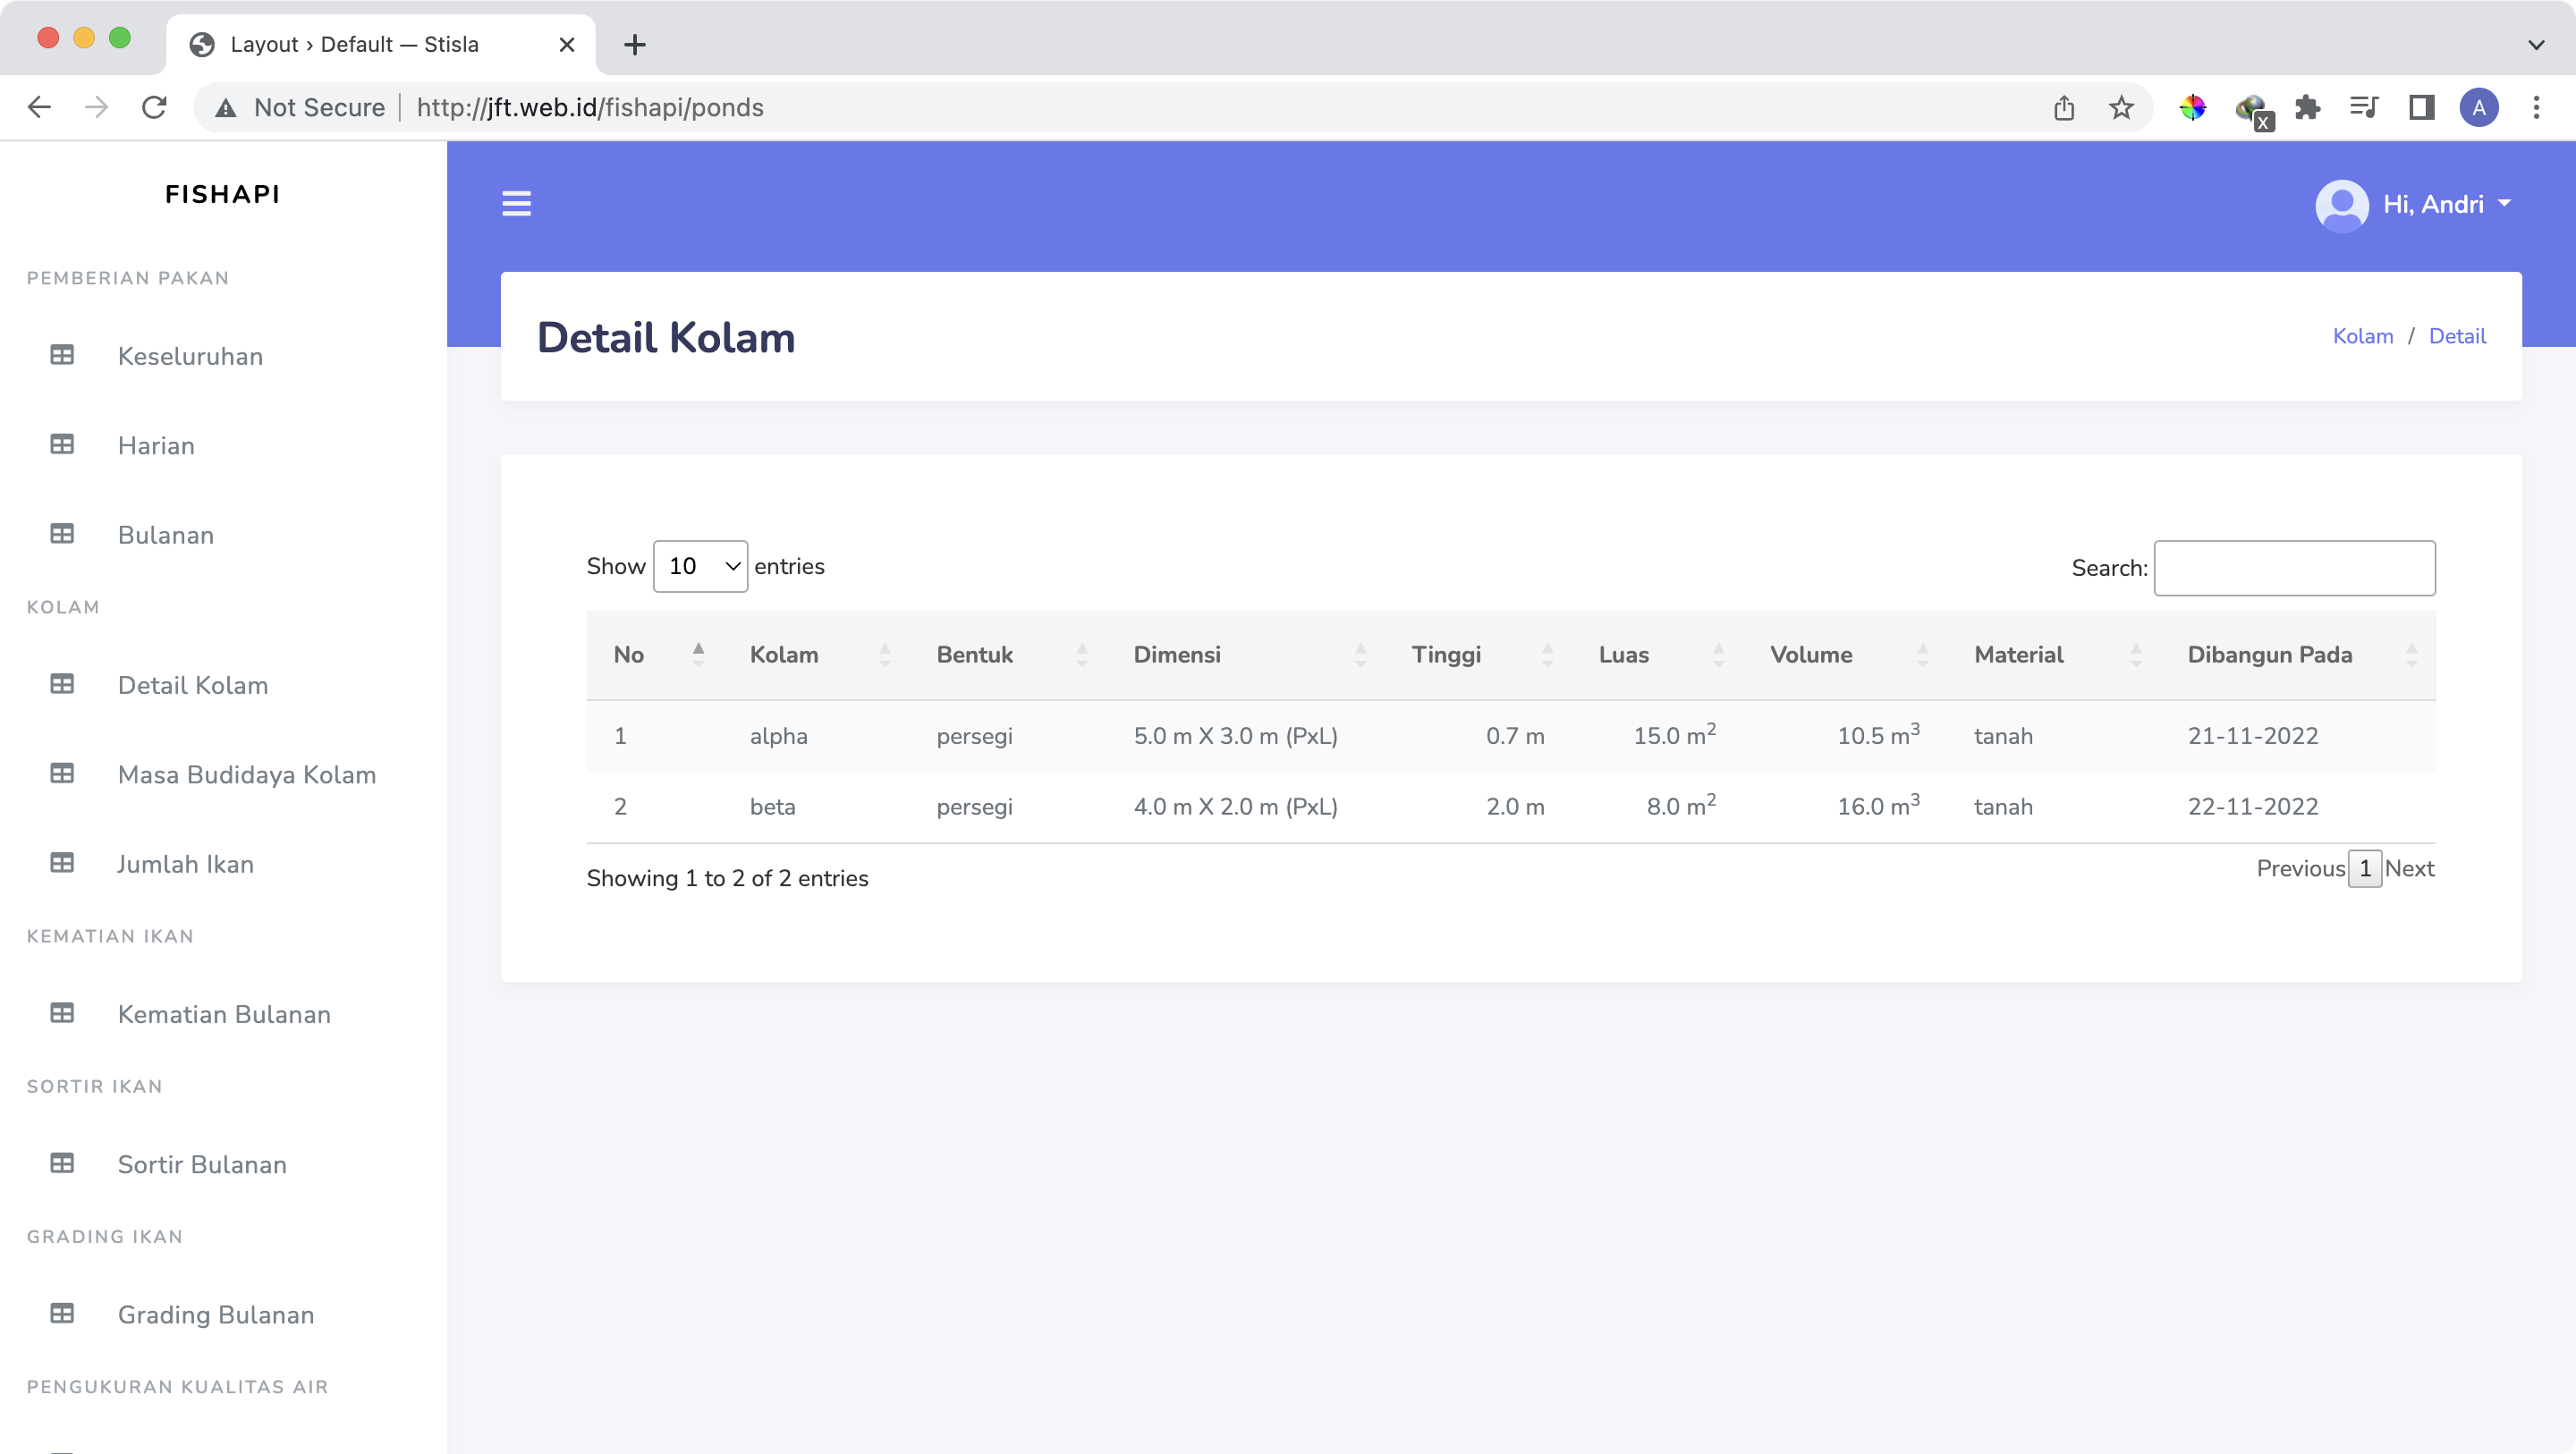
\includegraphics[width=1\textwidth]{gambar/Sprint03/view/view_detail_kolam}
	\caption{View detail kolam}
	\label{fig:view_detail_kolam}
\end{figure}
	
\end{enumerate}
%!TEX root = ./template-skripsi.tex

\subsection{Sprint 4 Report}
Berikut merupakan report dari sprint ke-4 yang dilakukan pada tanggal 15 juni - 21 juni 2022.

\begin{table}[H]
	\caption{\textit{Sprint-4 backlog}}
	\label{sprint4_backlog}
	\begin{tabular}{@{} |p{0.5cm}|p{5cm}|p{5cm}|p{2cm}| @{}}
		\hline
		\textbf{No} & \textbf{\textit{Story}} & \textbf{\textit{Task}} & \textbf{\textit{Status}} \\
		\hline
		1 & \multirow{3}{5cm}{Create, Read, Updte, dan Delete untuk Masa Budidaya Kolam} & Membarui desain database  & Completed\\
		\cline{1-1}\cline{3-4}
		2 & & Implementasi API aktifasi kolam & Completed\\
		\cline{1-1}\cline{3-4}
		3 & & Implementasi API deaktifasi kolam & Completed\\
		\cline{1-1}\cline{3-4}
		4 & & Implementasi API fetch list status kolam & Completed\\
		\cline{1-1}\cline{3-4}
		5 & & Implementasi API fetch musim budidaya per kolam & Completed\\
		\cline{1-1}\cline{3-4}
		6 & & Membuat view status budidaya semua kolam & Completed\\
		\cline{1-1}\cline{3-4}
		7 & & Membuat view list budidaya per kolam & Completed\\
		\cline{1-1}\cline{3-4}
		8 & & Membuat view detail budidaya & Completed\\
		\cline{1-1}\cline{3-4}
		\hline
	\end{tabular}
\end{table}

\begin{enumerate}[1.]



\item \textbf{Membarui desain database}

\begin{figure}[H]
	\centering
	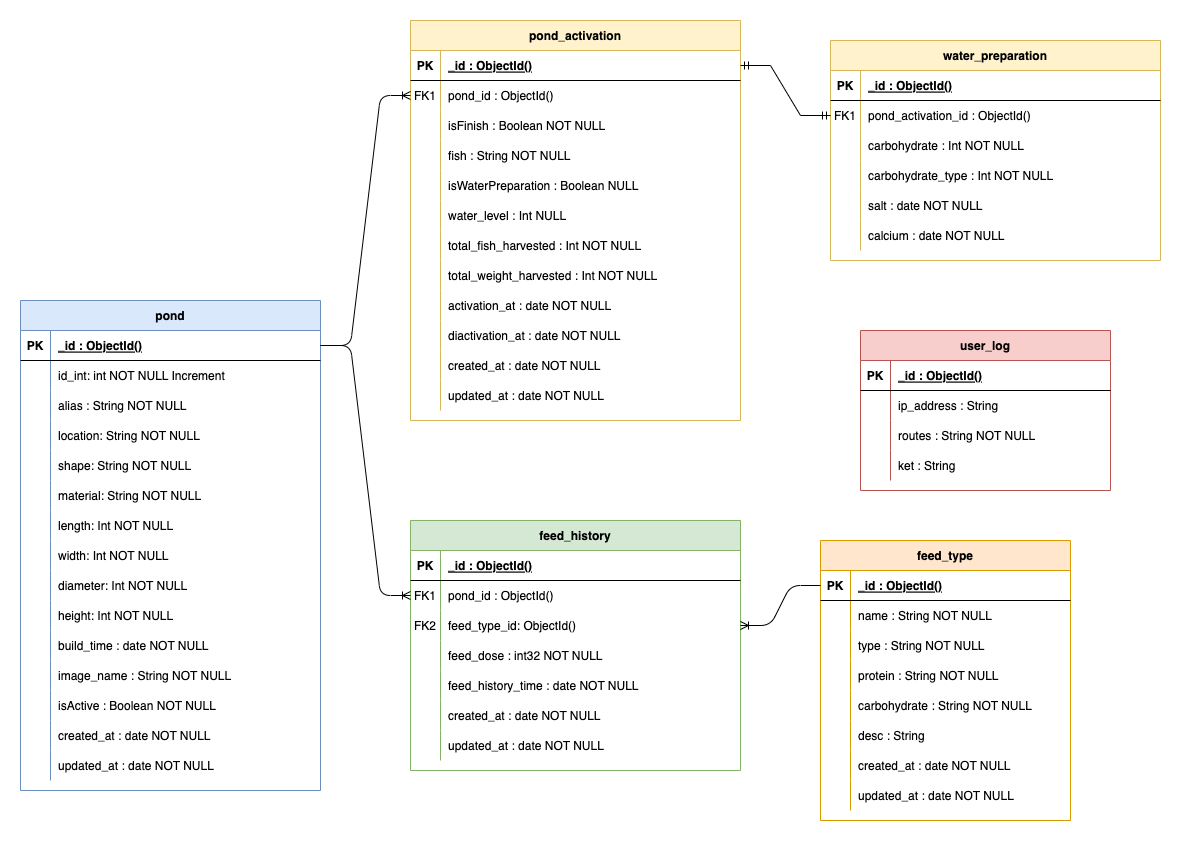
\includegraphics[height=0.7\textwidth]{gambar/Sprint04/diagram database/database}
	\caption{ERD Database Sprint-4}
	\label{fig:database_sprint4}
\end{figure}

Dengan berubahnya desain database diperlukan juga penambahan model pada source code, berikut perubahan pada source code model.

\begin{lstlisting}
# fishapi/database/model.py

class PondActivation(db.Document):
    id_int = db.IntField(required=True)
    pond_id = db.ReferenceField(Pond, required=True)
    isFinish = db.BooleanField(required=True, default=False)
    isWaterPreparation = db.BooleanField(required=True, default=False)
    water_level = db.FloatField(required=True, default=0)
    total_fish_harvested = db.IntField(required=True, default=0)
    total_weight_harvested = db.IntField(required=True, default=0)
    activated_at = db.DateTimeField(default=datetime.datetime.now)
    deactivated_at = db.DateTimeField(default=None)
    deactivated_description = db.StringField(default=None)
    constanta_oversize = db.FloatField(required=True, default=1.3)
    constanta_undersize = db.FloatField(required=True, default=0.7)
    created_at = db.DateTimeField(default=datetime.datetime.now)
    updated_at = db.DateTimeField(default=datetime.datetime.now)
\end{lstlisting}



\item \textbf{Implementasi API aktifasi kolam}

Perubahan terjadi pada controller API entry musim budidaya, berikut merupakan perubahan source code controller API entry musim budidaya.

\begin{lstlisting}
# fishapi/database/pondactivation.py

class PondActivationApi(Resource):
    def post(self, pond_id):
        pond = Pond.objects.get(id=pond_id)
        pipeline_year = {'$match': {'$expr': {'$and': [
                        {'$eq': ['$pond_id', {'$toObjectId': pond_id}]},
                        {'$eq': [{'$dateToString': {
                            'format': "%Y", 'date': "$created_at"}}, getYearToday()]},
        ]
        }}}
        list_pond_year = PondActivation.objects.aggregate(pipeline_year)
        list_pond_year = list(list_pond_year)
        id_int = len(list_pond_year) + 1
        if pond.isActive == True:
            response = {"message": "status pond is already active"}
            response = json.dumps(response, default=str)
            return Response(response, mimetype="application/json", status=400)
        fishes = request.form.get("fish", "[]")
        fishes = json.loads(fishes)
        if len(fishes) < 1:
            response = {"message": "There is no fish"}
            response = json.dumps(response, default=str)
            return Response(response, mimetype="application/json", status=400)
        isWaterPreparation = request.form.get("isWaterPreparation", False)
        if isWaterPreparation == "true":
            isWaterPreparation = True
        else:
            isWaterPreparation = False
        water_level = request.form.get("water_level", None)
        activated_at = request.form.get(
            "activated_at", datetime.datetime.now())
        pond_activation_data = {
            "id_int": id_int,
            "pond_id": pond_id,
            "isFinish": False,
            "isWaterPreparation": isWaterPreparation,
            "water_level": water_level,
            "activated_at": activated_at
        }
        pondActivation = PondActivation(**pond_activation_data).save()
        pondActivation_id = pondActivation.id
        if isWaterPreparation == True:
            carbohydrate = request.form.get("carbohydrate", None)
            carbohydrate_type = request.form.get("carbohydrate_type", None)
            salt = request.form.get("salt", None)
            calcium = request.form.get("calcium", None)
            water_preparation_data = {
                "pond_activation_id": pondActivation_id,
                "carbohydrate": carbohydrate,
                "carbohydrate_type": carbohydrate_type,
                "salt": salt,
                "calcium": calcium,
            }
            water_preparation = WaterPreparation(
                **water_preparation_data).save()
        pond.update(**{"isActive": True})
        for fish in fishes:
            # save fish log
            data = {
                "pond_id": pond_id,
                "pond_activation_id": pondActivation_id,
                "type_log": "activation",
                "fish_type": fish['type'],
                "fish_amount": fish['amount'],
                "fish_total_weight": fish['weight']
            }
            fishlog = FishLog(**data).save()
        response = {"message": "success to activation pond"}
        response = json.dumps(response, default=str)
        return Response(response, mimetype="application/json", status=200)
\end{lstlisting}

Kode tersebut adalah sebuah fungsi dalam sebuah REST API yang bertujuan untuk mengaktifkan kolam ikan. Pada awal fungsi, dilakukan pencarian kolam ikan berdasarkan id kolam yang diberikan.

Selanjutnya, dilakukan operasi agregasi MongoDB untuk mencari data aktivasi pada tahun ini dengan menggunakan metode \$match dan memanfaatkan fungsi agregasi lainnya seperti \$and, \$eq, \$dateToString, dan getYearToday(). Hasil agregasi kemudian disimpan dalam variabel list\_pond\_year.

Selanjutnya, variabel id\_int dihitung berdasarkan panjang dari list\_pond\_year ditambah 1. Kemudian, dilakukan beberapa validasi seperti memeriksa apakah kolam sudah aktif atau belum, dan apakah terdapat ikan yang akan dimasukkan ke dalam kolam.

Jika semua validasi telah dilakukan, data aktivasi kolam akan disimpan dalam database, lalu dilakukan pembaruan pada status kolam menjadi aktif. Data ikan yang dimasukkan ke dalam kolam juga akan disimpan dalam bentuk log pada tabel FishLog.

Terakhir, fungsi mengembalikan respons dalam format JSON yang berisi pesan berhasil atau gagalnya aktivasi kolam.

Berikut merupakan form untuk entry musim budidaya.

\begin{longtable}{| l | p{5cm} | p{5cm} |}
\caption{Form entry musim budidaya kolam.\label{table:form_entry_musim_budidaya}}\\

\hline
\multicolumn{1}{|c|}{\textbf{Form}} & \multicolumn{1}{|c|}{\textbf{Jenis Data}} & \multicolumn{1}{|c|}{\textbf{Deskripsi}}\\
\hline
\endfirsthead

\hline
\multicolumn{3}{|c|}{Lanjutan Tabel \ref{table:form_entry_musim_budidaya}}\\
\hline
\multicolumn{1}{|c|}{\textbf{Form}} & \multicolumn{1}{|c|}{\textbf{Jenis Data}} & \multicolumn{1}{|c|}{\textbf{Deskripsi}}\\
\hline
\endhead

                                          
fish               & REQUIRED STRING FORMAT list(dict()) jenis ikan : {[}"nila merah", "nila hitam", "lele", "patin", "mas"{]} ex: "{[}\{"lele": 100\},\{"patin":200\}{]}" & jenis ikan dan jumlah ikan                             \\ \hline
isWaterPreparation & REQUIRED STRING BOOLEAN                                                                                                                               & variable bila aktifasi kolam menggunakan preparasi air \\ \hline
water\_level       & REQUIRED DOUBLE                                                                                                                                       & ketinggian air dalam meter (m)                         \\ \hline
activated\_at      & OPTIONAL STRING DATE FORMAT : isodate()                                                                                                               & timestamp aktifasi kolam                               \\ \hline
carbohydrate       & REQUIRED INTEGER IF isWaterPreparation == True                                                                                                        & banyak karbohidrat dalam (Gram/ml)                     \\ \hline
carbohydrate\_type & REQUIRED STRING IF isWaterPreparation == True VALUE : {[}"gula", "molase", "trigu", "tapioka",{]}                                                     & jenis karbohidrat yang di gunakan                      \\ \hline
salt               & REQUIRED INTEGER IF isWaterPreparation == True                                                                                                        & berat garam yang di gunakan (Kg)                       \\ \hline
calcium            & REQUIRED INTEGER IF isWaterPreparation == True                                                                                                        & berat kapur yang di gunakan (gram)                     \\ \hline

\end{longtable}


Tabel di atas berisi informasi tentang parameter yang harus diisi atau opsional dalam aktivasi atau memulai musim budidaya kolam ikan. Berikut adalah penjelasan masing-masing kolom pada tabel tersebut:

\begin{enumerate}
\item Form: Merupakan nama parameter yang harus diisi atau opsional dalam aktivasi kolam ikan.
\item Jenis Data: Menjelaskan jenis data yang harus diisi pada parameter tersebut. Contohnya, string, boolean, integer, atau double.
\item Deskripsi: Berisi deskripsi singkat tentang informasi yang harus diisi pada parameter tersebut.
\end{enumerate}

Beberapa contoh parameter yang harus diisi pada aktivasi kolam ikan di antaranya adalah jenis ikan dan jumlahnya, ketinggian air dalam meter, dan variable bila aktivasi kolam menggunakan preparasi air. Ada juga parameter yang opsional, seperti timestamp aktifasi kolam. Selain itu, ada parameter yang harus diisi jika variable bila aktivasi kolam menggunakan preparasi air diaktifkan, seperti banyak karbohidrat dalam gram/ml dan jenis karbohidrat yang digunakan. Ada juga parameter yang harus diisi jika menggunakan kapur atau garam dalam preparasi air, yaitu berat kapur dan berat garam yang digunakan. Semua parameter ini harus diisi dengan format yang sudah ditentukan pada kolom Jenis Data.

Berikut merupakan hasil test request dari API aktivasi kolam.

cURL:

\begin{lstlisting}
curl --location -g 'http://jft.web.id/fishapi/api/ponds/{pond_id}/activation' \
--form 'fish="[{\"lele\": 100},{\"patin\":200}]"' \
--form 'isWaterPreparation="false"' \
--form 'water_level="100"'
\end{lstlisting}

response json:

\begin{lstlisting}
{
  "message": "success to activation pond"
}
\end{lstlisting}



\item \textbf{Implementasi API deaktifasi kolam}

Penambahan terjadi pada controller API entry musim budidaya, berikut merupakan perubahan source code controller API entry panen musim budidaya.

\begin{lstlisting}
# fishapi/database/pondactivation.py

class PondDeactivationApi(Resource):
    def post(self, pond_id):
        pond = Pond.objects.get(id=pond_id)
        if pond.isActive == False:
            response = {"message": "status pond is already not active"}
            response = json.dumps(response, default=str)
            return Response(response, mimetype="application/json", status=400)
        # get last pond_activation
        pond_activation = PondActivation.objects(
            pond_id=pond_id, isFinish=False).order_by('-activated_at').first()
        fishes = request.form.get("fish", "[]")
        fishes = json.loads(fishes)
        total_fish_harvested = 0
        total_weight_harvested = 0
        for fish in fishes:
            # save fish log
            data = {
                "pond_id": pond_id,
                "pond_activation_id": pond_activation.id,
                "type_log": "deactivation",
                "fish_type": fish['type'],
                "fish_amount": fish['amount'],
                "fish_total_weight": fish['weight']
            }
            total_fish_harvested += fish['amount']
            total_weight_harvested += fish['weight']
            fishlog = FishLog(**data).save()
            print(data)
        print(total_fish_harvested)
        print(total_weight_harvested)
        # get args form data
        # update pond_activation
        pond_deactivation_data = {
            "isFinish": True,
            "total_fish_harvested": total_fish_harvested,
            "total_weight_harvested": total_weight_harvested,
            "deactivated_at": request.form.get("deactivated_at", datetime.datetime.now()),
            "deactivated_description": "Normal"
        }
        pond_activation.update(**pond_deactivation_data)
        # update pond isActive
        pond.update(**{"isActive": False})
        response = {"message": "success to deactivation pond"}
        response = json.dumps(response, default=str)
        return Response(response, mimetype="application/json", status=200)
\end{lstlisting}

Kode ini merupakan sebuah kelas Python dengan nama PondDeactivationApi yang diturunkan dari kelas Resource. Kelas ini memiliki satu method yaitu post() yang mengambil satu argumen yaitu pond\_id.

Dalam method post(), dilakukan pengambilan data Pond dengan id tertentu yang diberikan sebagai argumen. Kemudian, jika atribut isActive pada objek Pond bernilai False, maka akan dikembalikan respons dengan pesan "status pond is already not active" dan status kode 400.

Selanjutnya, dilakukan pengambilan PondActivation terakhir yang memiliki pond\_id tertentu dan isFinish bernilai False. Kemudian, dilakukan pengolahan data ikan dengan mengambil nilai dari form data "fish", yang kemudian di-parse dari string JSON menjadi list Python. Dalam loop for, dilakukan penyimpanan data FishLog untuk setiap ikan yang terdapat dalam list fishes.

Setelah itu, dilakukan pembaruan data pada objek PondActivation dengan mengubah nilai atribut isFinish menjadi True dan menambahkan data mengenai total jumlah ikan yang dipanen (total\_fish\_harvested) dan total berat ikan yang dipanen (total\_weight\_harvested), serta waktu dan deskripsi pada saat deaktivasi. Selanjutnya, dilakukan pembaruan data pada objek Pond dengan mengubah nilai atribut isActive menjadi False.

Akhirnya, dilakukan pembuatan respons dengan pesan "success to deactivation pond" dan status kode 200. Pesan respons dan data lainnya kemudian di-serialize menjadi string JSON dengan menggunakan modul json dan dikembalikan dalam bentuk response dengan tipe konten "application/json".

Berikut merupakan form untuk entry panen musim budidaya.

\begin{longtable}{| l | p{5cm} | p{5cm} |}
\caption{Form entry panen musim budidaya kolam.\label{table:form_entry_panen_musim_budidaya}}\\

\hline
\multicolumn{1}{|c|}{\textbf{Form}} & \multicolumn{1}{|c|}{\textbf{Jenis Data}} & \multicolumn{1}{|c|}{\textbf{Deskripsi}}\\
\hline
\endfirsthead

\hline
\multicolumn{3}{|c|}{Lanjutan Tabel \ref{table:form_entry_musim_budidaya}}\\
\hline
\multicolumn{1}{|c|}{\textbf{Form}} & \multicolumn{1}{|c|}{\textbf{Jenis Data}} & \multicolumn{1}{|c|}{\textbf{Deskripsi}}\\
\hline
\endhead


total\_fish\_harvested   & REQUIRED INTEGER                                        & banyak ikan yang di angkat        \\ \hline
total\_weight\_harvested & REQUIRED INTEGER                                        & berat seluruh ikan yang di angkat \\ \hline
diactived\_at            & OPTIONAL STRING DATE FORMAT : isodate() DEFAULT : now() & timestamp diaktifasi kolam        \\ \hline

\end{longtable}

Tabel ini terdiri dari 3 baris, dimana setiap baris merepresentasikan sebuah parameter yang dapat digunakan dalam suatu API. Setiap baris terdiri dari 3 kolom yaitu:

\begin{enumerate}
\item Form : Merupakan nama parameter yang digunakan dalam API.
\item Jenis Data : Menjelaskan jenis data yang diterima oleh parameter tersebut. Pada tabel ini, Jenis Data terdiri dari REQUIRED INTEGER dan OPTIONAL STRING DATE FORMAT : isodate() DEFAULT : now().
\begin{enumerate}
\item REQUIRED INTEGER artinya bahwa parameter tersebut wajib diisi dengan nilai berupa bilangan bulat (integer).
\item OPTIONAL STRING DATE FORMAT : isodate() DEFAULT : now() artinya bahwa parameter tersebut bersifat opsional dan dapat diisi dengan nilai berupa string yang merepresentasikan tanggal dan waktu dalam format ISO (isodate), dengan nilai default saat tidak diisi adalah waktu saat ini.
\end{enumerate}
\item Deskripsi : Menjelaskan secara singkat tentang parameter tersebut. Pada tabel ini, Deskripsi menjelaskan tentang banyak ikan yang diangkat, berat seluruh ikan yang diangkat, dan timestamp diaktifasi kolam.
\end{enumerate}

Berikut merupakan hasil test request dari API deaktifasi/panen masa budidaya kolam.

cURL:
\begin{lstlisting}
curl --location -g 'http://jft.web.id/fishapi/api/ponds/{pond_id}/diactivation' \
--form 'total_fish_harvested="300"' \
--form 'total_weight_harvested="3000"'
\end{lstlisting}

response json:
\begin{lstlisting}
{
  "message": "success to diactivation pond"
}
\end{lstlisting}



\item \textbf{Implementasi API fetch list status kolam}

Penambahan terjadi pada controller API fetch list status kolam, berikut merupakan perubahan source code controller API fetch list status kolam.

\begin{lstlisting}
# fishapi/database/pondactivation.py

class PondsStatusApi(Resource):
    def get(self):
        pipline = [
            {'$lookup': {
                'from': 'pond_activation',
                'let': {"pondid": "$_id"},
                'pipeline': [
                    {'$match': {'$expr': {'$and': [
                        {'$eq': ['$pond_id', '$$pondid']},
                    ]}}},
                    {'$lookup': {
                        'from': 'water_preparation',
                        'let': {"pond_activation_id": "$_id"},
                        'pipeline': [
                            {'$match': {
                                '$expr': {'$eq': ['$pond_activation_id', '$$pond_activation_id']}}},
                            {"$project": {
                                "created_at": 0,
                                "updated_at": 0,
                            }}
                        ],
                        'as': 'water_preparation'
                    }},
                    {"$addFields": {
                        "water_preparation": {"$first": "$water_preparation"}
                    }},
                    {"$project": {
                        "pond_id": 0,
                        "feed_type_id": 0,
                        "created_at": 0,
                        "updated_at": 0,
                    }}
                ],
                'as': 'pond_activation_list'
            }},
            {"$addFields": {
                "total_activation": {"$size": "$pond_activation_list"},
            }},
            {"$project": {
                "location": 0,
                "shape": 0,
                "material": 0,
                "length": 0,
                "width": 0,
                "diameter": 0,
                "height": 0,
                "image_name": 0,
                "pond_activation_list": 0,
                "updated_at": 0,
                "created_at": 0,
            }}
        ]
        ponds = Pond.objects().aggregate(pipline)
        response = list(ponds)
        response = json.dumps(response, default=str)
        return Response(response, mimetype="application/json", status=200)
\end{lstlisting}

Class ini memiliki sebuah method GET, yang berfungsi untuk mengambil data status kolam ikan dari database.

Method GET ini menggunakan sebuah pipeline pada MongoDB, yaitu pipline yang terdiri dari beberapa tahap, yaitu:

\begin{enumerate}
\item Lookup: Melakukan join dengan tabel "pond\_activation" berdasarkan \_id kolam ikan pada tabel "pond". Join ini dilakukan menggunakan operasi \$lookup pada MongoDB.

\item Match: Melakukan filtering pada data yang telah di-join dengan tabel "pond\_activation", dengan kondisi bahwa pond\_id pada tabel "pond\_activation" harus sama dengan \_id pada tabel "pond".

\item Lookup: Melakukan join dengan tabel "water\_preparation" berdasarkan pond\_activation\_id pada tabel "pond\_activation". Join ini dilakukan menggunakan operasi \$lookup pada MongoDB.

\item Match: Melakukan filtering pada data yang telah di-join dengan tabel "water\_preparation", dengan kondisi bahwa pond\_activation\_id pada tabel "water\_preparation" harus sama dengan \_id pada tabel "pond\_activation".

\item Project: Mengembalikan data pada tabel "water\_preparation" ke dalam variabel "water\_preparation" pada tabel "pond\_activation".

\item Project: Menghilangkan beberapa kolom pada tabel "pond\_activation".

\item AddFields: Menambahkan kolom "total\_activation" pada tabel "pond".

\item Project: Menghilangkan beberapa kolom pada tabel "pond".
\end{enumerate}

Setelah pipline tersebut dijalankan, hasilnya akan di-serialize menjadi format JSON, dan kemudian dikirimkan sebagai response dengan HTTP status code 200.

Berikut merupakan hasil test request dari API fetch list status kolam.

cURL:
\begin{lstlisting}
curl --location 'http://jft.web.id/fishapi/api/ponds/status'
\end{lstlisting}

response json:
\begin{lstlisting}
[
  {
    "_id": "625d7026a9a73e090c65cda1",
    "id_int": 2,
    "alias": "alpha",
    "build_at": "2022-04-18 21:05:26.183000",
    "isActive": true,
    "total_activation": 2
  },
  {
    "_id": "625d7033a9a73e090c65cda2",
    "id_int": 3,
    "alias": "beta",
    "build_at": "2022-04-18 21:05:39.608000",
    "isActive": false,
    "total_activation": 0
  },
  {
    "_id": "62a62163e445ffb9c5f746f3",
    "id_int": 4,
    "alias": "charlie",
    "build_at": "2022-06-13 00:24:51.473000",
    "isActive": false,
    "total_activation": 0
  },
  {
    "_id": "62a955888911334402ddb3b3",
    "id_int": 5,
    "alias": "delta",
    "build_at": "2022-06-15 10:44:08.180000",
    "isActive": false,
    "total_activation": 0
  },....
]
\end{lstlisting}



\item \textbf{Implementasi API fetch musim budidaya per kolam}

Penambahan terjadi pada controller API fetch musim budidaya per kolam, berikut merupakan perubahan source code controller API musim budidaya per kolam.

\begin{lstlisting}
# fishapi/database/pondactivation.py

class PondStatusApi(Resource):
    def get(self, pond_id):
        pond_objects = Pond.objects.get(id=pond_id)
        pipline = [
            {'$match': {'$expr': {'$eq': ['$_id', {'$toObjectId': pond_id}]}}},
            {'$lookup': {
                'from': 'pond_activation',
                'let': {"pondid": "$_id"},
                'pipeline': [
                    {'$match': {'$expr': {'$and': [
                        {'$eq': ['$pond_id', '$$pondid']},
                    ]}}},
                    {"$sort": {"activated_at": -1}},
                    {'$lookup': {
                        'from': 'fish_log',
                        'let': {"pond_activation_id": "$_id"},
                        'pipeline': [
                            {'$match': {
                                '$expr': {'$and': [
                                    {'$eq': ['$pond_activation_id',
                                     '$$pond_activation_id']},
                                    {'$eq': ['$type_log', 'activation']},
                                ]}
                            }},
                            {"$project": {
                                "created_at": 0,
                                "updated_at": 0,
                            }},
                            {"$group": {
                                "_id": "$fish_type",
                                "fish_type": {"$first": "$fish_type"},
                                "fish_amount": {"$sum": "$fish_amount"},
                                "fish_total_weight": {"$sum": "$fish_total_weight"}
                            }},
                            {"$sort": {"fish_type": -1}},
                            {"$project": {
                                "_id": 0,
                            }},
                        ],
                        'as': 'fish_stock'
                    }},
                    {'$lookup': {
                        'from': 'fish_log',
                        'let': {"pond_activation_id": "$_id"},
                        'pipeline': [
                            {'$match': {
                                '$expr': {'$and': [
                                    {'$eq': ['$pond_activation_id',
                                     '$$pond_activation_id']},
                                    {'$ne': ['$type_log', 'deactivation']},
                                ]}
                            }},
                            {"$project": {
                                "created_at": 0,
                                "updated_at": 0,
                            }},
                            {"$group": {
                                "_id": "$fish_type",
                                "fish_type": {"$first": "$fish_type"},
                                "fish_amount": {"$sum": "$fish_amount"}
                            }},
                            {"$sort": {"fish_type": -1}},
                            {"$project": {
                                "_id": 0,
                            }},
                        ],
                        'as': 'fish_live'
                    }},
                    {'$lookup': {
                        'from': 'fish_log',
                        'let': {"pond_activation_id": "$_id"},
                        'pipeline': [
                            {'$match': {
                                '$expr': {'$and': [
                                    {'$eq': ['$pond_activation_id',
                                             '$$pond_activation_id']},
                                    {'$eq': ['$type_log', 'death']},
                                ]}
                            }},
                            {"$project": {
                                "created_at": 0,
                                "updated_at": 0,
                            }},
                            {"$group": {
                                "_id": "$fish_type",
                                "fish_type": {"$first": "$fish_type"},
                                "fish_amount": {"$sum": "$fish_amount"}
                            }},
                            {"$sort": {"fish_type": -1}},
                            {"$project": {
                                "_id": 0,
                            }},
                        ],
                        'as': 'fish_death'
                    }},
                    {'$lookup': {
                        'from': 'fish_log',
                        'let': {"pond_activation_id": "$_id"},
                        'pipeline': [
                            {'$match': {
                                '$expr': {'$and': [
                                    {'$eq': ['$pond_activation_id',
                                     '$$pond_activation_id']},
                                    {'$eq': ['$type_log', 'deactivation']},
                                ]}
                            }},
                            {"$project": {
                                "created_at": 0,
                                "updated_at": 0,
                            }},
                            {"$group": {
                                "_id": "$fish_type",
                                "fish_type": {"$first": "$fish_type"},
                                "fish_amount": {"$sum": "$fish_amount"},
                                "fish_total_weight": {"$sum": "$fish_total_weight"},
                            }},
                            {"$sort": {"fish_type": -1}},
                            {"$project": {
                                "_id": 0,
                            }},
                        ],
                        'as': 'fish_harvested'
                    }},
                    {'$lookup': {
                        'from': 'feed_history',
                        'let': {"pond_activation_id": "$_id"},
                        'pipeline': [
                            {'$match': {
                                '$expr': {'$and': [
                                    {'$eq': ['$pond_activation_id',
                                             '$$pond_activation_id']},
                                ]}
                            }},
                        ],
                        'as': 'feed_history'
                    }},
                    {'$lookup': {
                        'from': 'water_preparation',
                        'let': {"pond_activation_id": "$_id"},
                        'pipeline': [
                            {'$match': {
                                '$expr': {'$eq': ['$pond_activation_id', '$$pond_activation_id']}}},
                            {"$project": {
                                "created_at": 0,
                                "updated_at": 0,
                            }}
                        ],
                        'as': 'water_preparation'
                    }},
                    {"$addFields": {
                        "water_preparation": {"$first": "$water_preparation"},
                        "total_fish": {"$sum": "$fish_live.fish_amount"},
                        "survival_rate": {"$cond": [
                            {"$eq": [{"$sum": "$fish_stock.fish_amount"}, 0]},
                            0,
                            {"$multiply": [{"$divide": [{"$sum": "$fish_live.fish_amount"}, {
                                "$sum": "$fish_stock.fish_amount"}]}, 100]}
                        ]},
                        "weight_growth": {"$subtract": [{"$sum": "$fish_harvested.fish_total_weight"}, {"$sum": "$fish_stock.fish_total_weight"}]},
                        "total_dose": {"$sum": "$feed_history.feed_dose"},
                        # "fcr": {"$sum": {"$divide": [{"$sum": "$fish_live.fish_amount"}, {"$sum": "$fish_stock.fish_amount"}]}},
                    }},
                    {"$addFields": {
                        "fcr": {"$cond": [
                            {"$eq": [{"$sum": "$total_dose"}, 0]},
                            0,
                            {"$sum": {"$divide": [
                                "$weight_growth", "$total_dose"]}}
                        ]},
                    }},
                    {"$project": {
                        "pond_id": 0,
                        "feed_history": 0,
                        "feed_type_id": 0,
                        "created_at": 0,
                        "updated_at": 0,
                    }}
                ],
                'as': 'pond_activation_list'
            }},
            {"$addFields": {
                "total_activation": {"$size": "$pond_activation_list"},
                "pond_activation_list": '$pond_activation_list',

            }},
            {"$project": {
                "location": 0,
                "shape": 0,
                "material": 0,
                "length": 0,
                "width": 0,
                "diameter": 0,
                "height": 0,
                "image_name": 0,
                "updated_at": 0,
                "created_at": 0,
            }}
        ]
        ponds = Pond.objects().aggregate(pipline)
        ponds = list(ponds)
        ponds = dict(ponds[0])
        response = json.dumps(ponds, default=str)
        return Response(response, mimetype="application/json", status=200)
\end{lstlisting}

Kode diatas adalah sebuah API untuk mengembalikan data status kolam ikan. Ketika API ini diakses dengan GET request, akan mengembalikan data status dari kolam ikan dengan id yang diberikan sebagai parameter. Data tersebut meliputi informasi tentang stok ikan hidup, ikan yang mati, ikan yang dipanen, dan sebagainya.

Seluruh data status kolam ikan yang dibutuhkan diperoleh dengan satu query melalui pipeline. Pipeline tersebut terdiri dari beberapa operasi seperti \$match, \$lookup, \$group, dan \$addFields yang digunakan untuk menggabungkan data dari beberapa tabel berbeda dan melakukan pengolahan data.

Setelah data berhasil diperoleh melalui pipeline, data tersebut akan dikembalikan dalam format JSON sebagai response dari GET request pada API ini.

Berikut merupakan hasil test request dari API fetch musim budidaya per kolam.

cURL:
\begin{lstlisting}
curl --location -g 'http://jft.web.id/fishapi/api/ponds/status/{pond_id}'
\end{lstlisting}

response json:
\begin{lstlisting}
{
  "_id": "625d7026a9a73e090c65cda1",
  "id_int": 2,
  "alias": "alpha",
  "build_at": "2022-04-18 21:05:26.183000",
  "isActive": true,
  "pond_activation_list": [
    {
      "_id": "62af3d637cf22faa567235ad",
      "isFinish": true,
      "fish": [
        {
          "lele": 100
        },
        {
          "patin": 200
        }
      ],
      "isWaterPreparation": true,
      "water_level": 100,
      "total_fish_harvested": 300,
      "total_weight_harvested": 3000,
      "activated_at": "2022-06-19 22:14:43.952000",
      "diactivated_at": "2022-06-19 23:10:03.469000",
      "water_preparation": {
        "_id": "62af3d637cf22faa567235ae",
        "pond_activation_id": "62af3d637cf22faa567235ad",
        "carbohydrate": 100,
        "carbohydrate_type": "gula",
        "salt": 100,
        "calcium": 100
      }
    },
    {
      "_id": "62af4c24f6a3ffba25a6be6a",
      "isFinish": false,
      "fish": [
        {
          "lele": 100
        },
        {
          "patin": 200
        }
      ],
      "isWaterPreparation": false,
      "water_level": 100,
      "total_fish_harvested": 0,
      "total_weight_harvested": 0,
      "activated_at": "2022-06-19 23:17:40.501000"
    }
  ],
  "total_activation": 2
}
\end{lstlisting}

\item \textbf{Membuat view status budidaya semua kolam}

\begin{figure}[H]
	\centering
	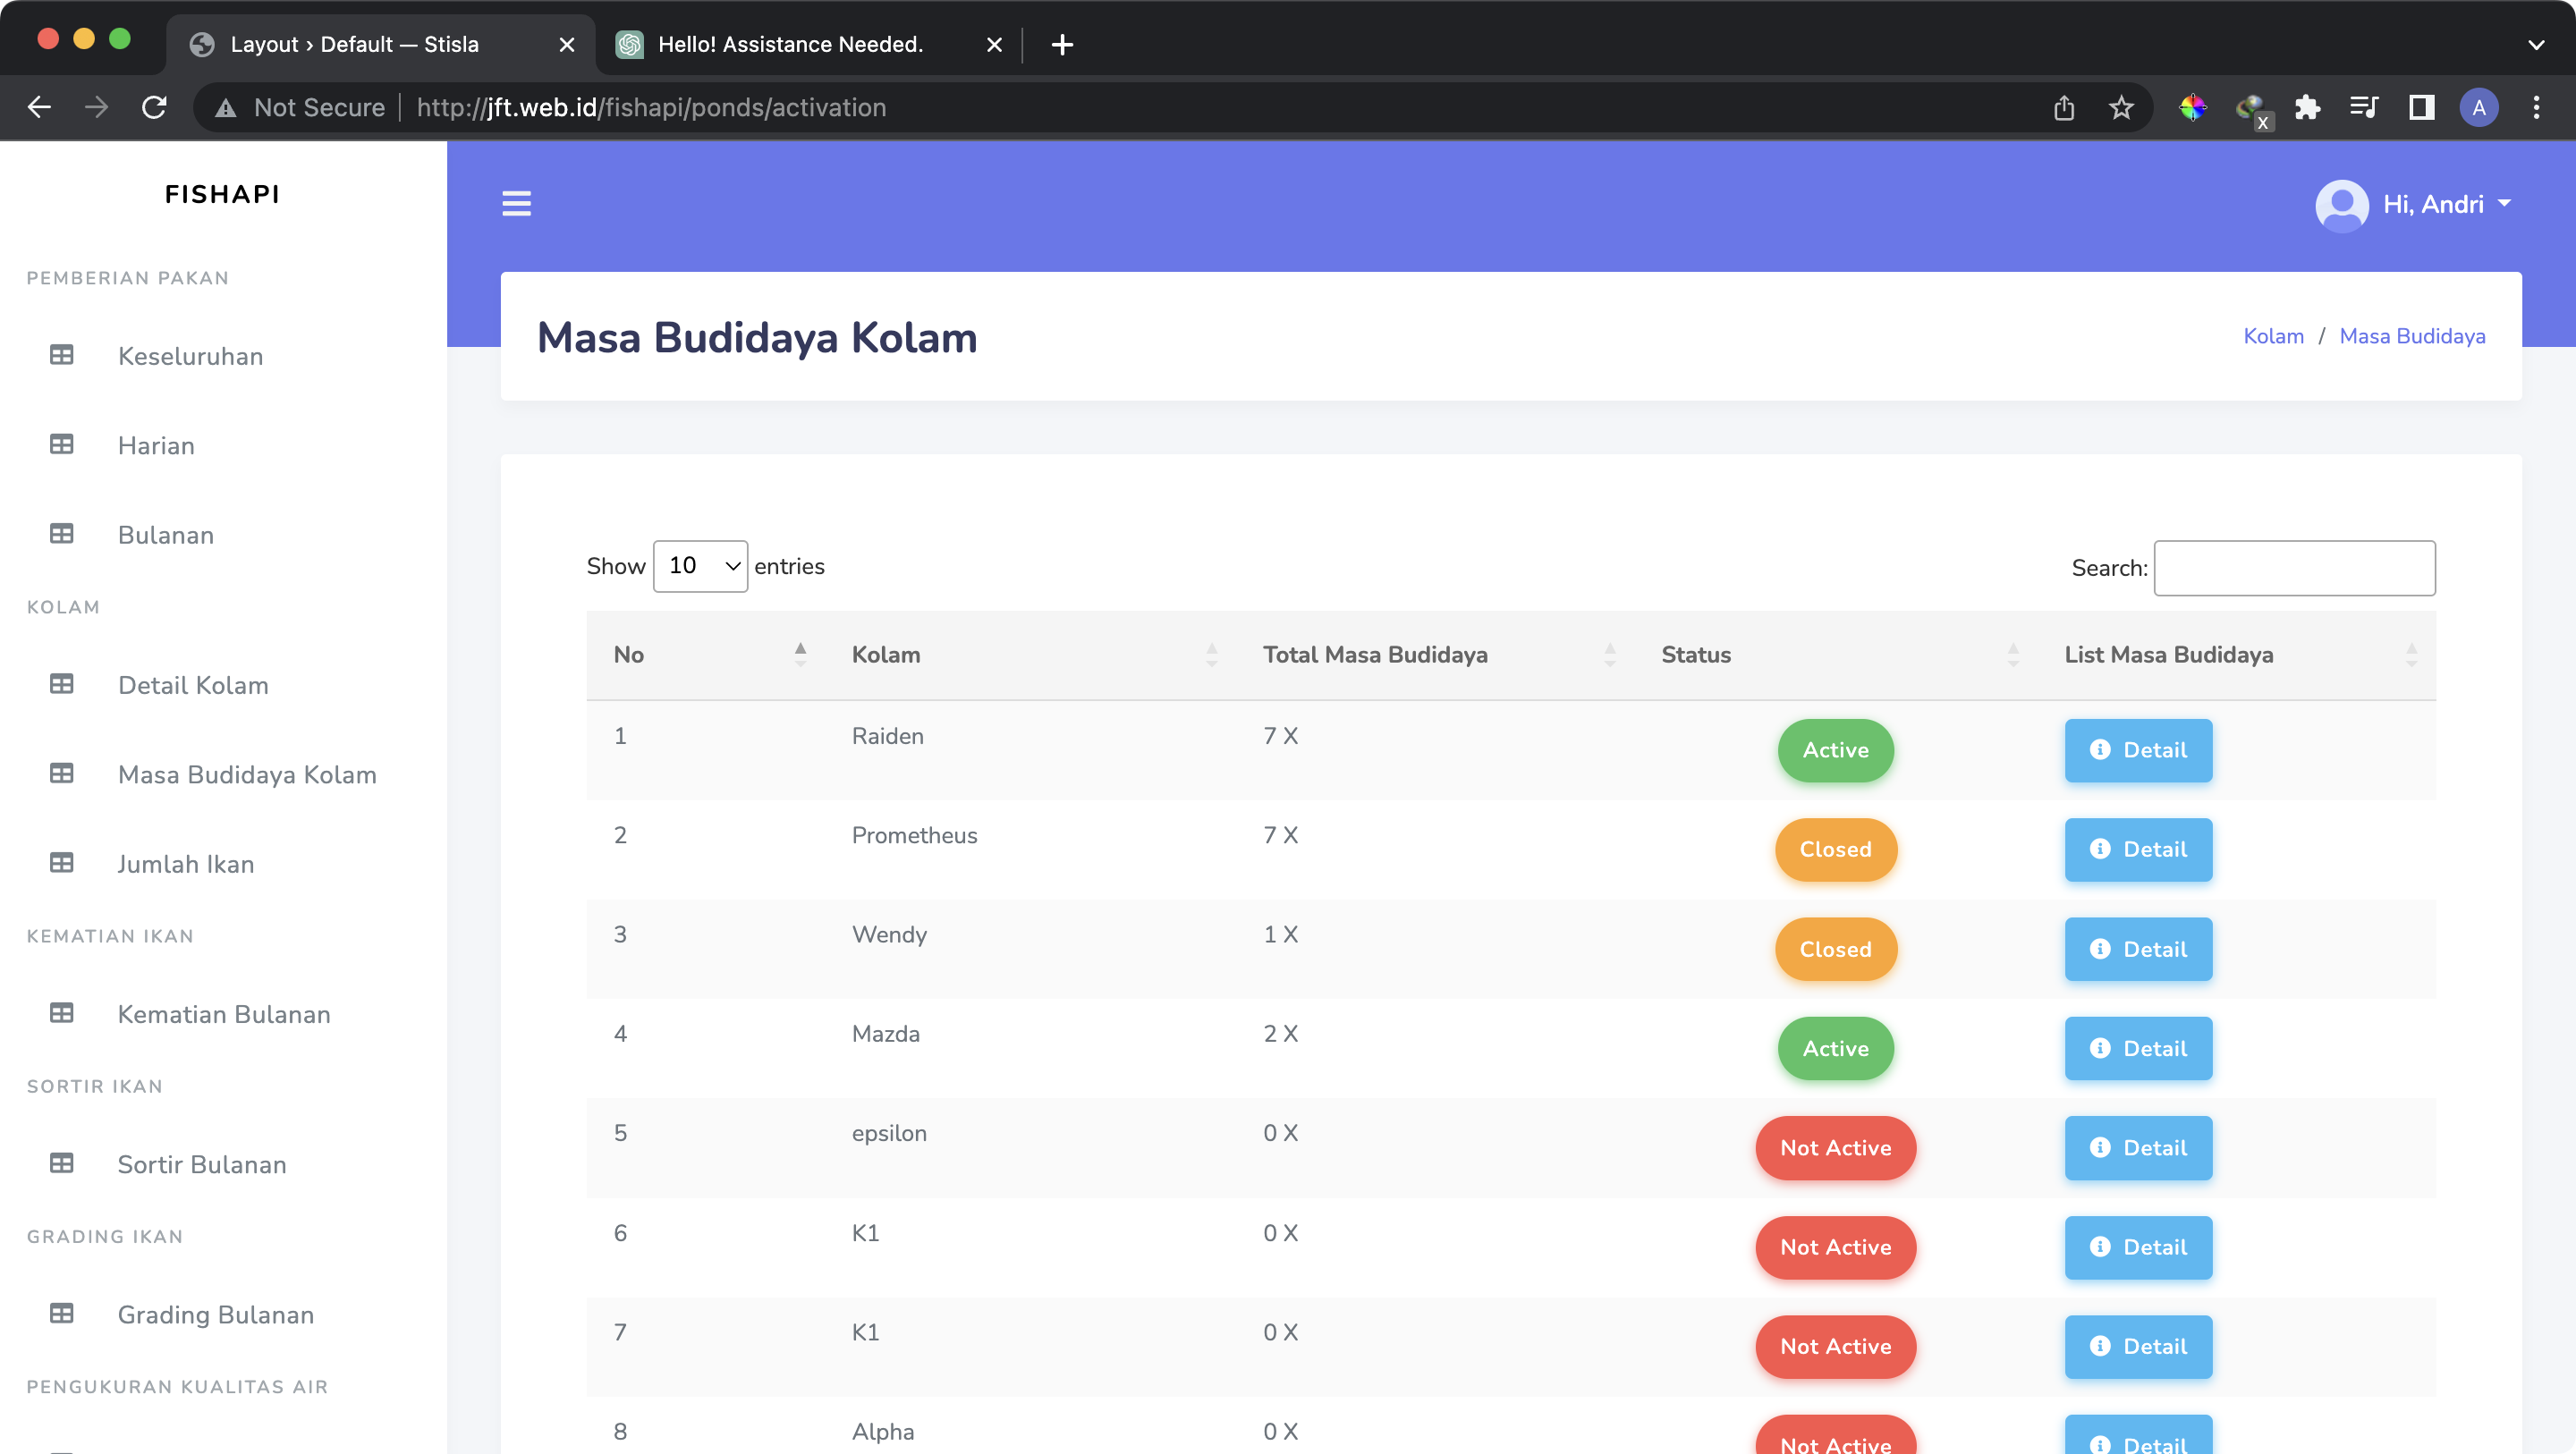
\includegraphics[width=1\textwidth]{gambar/Sprint04/view/view_status_kolam}
	\caption{View status kolam}
	\label{fig:view_status_kolam}
\end{figure}


\item \textbf{Membuat view list budidaya per kolam}
\begin{figure}[H]
	\centering
	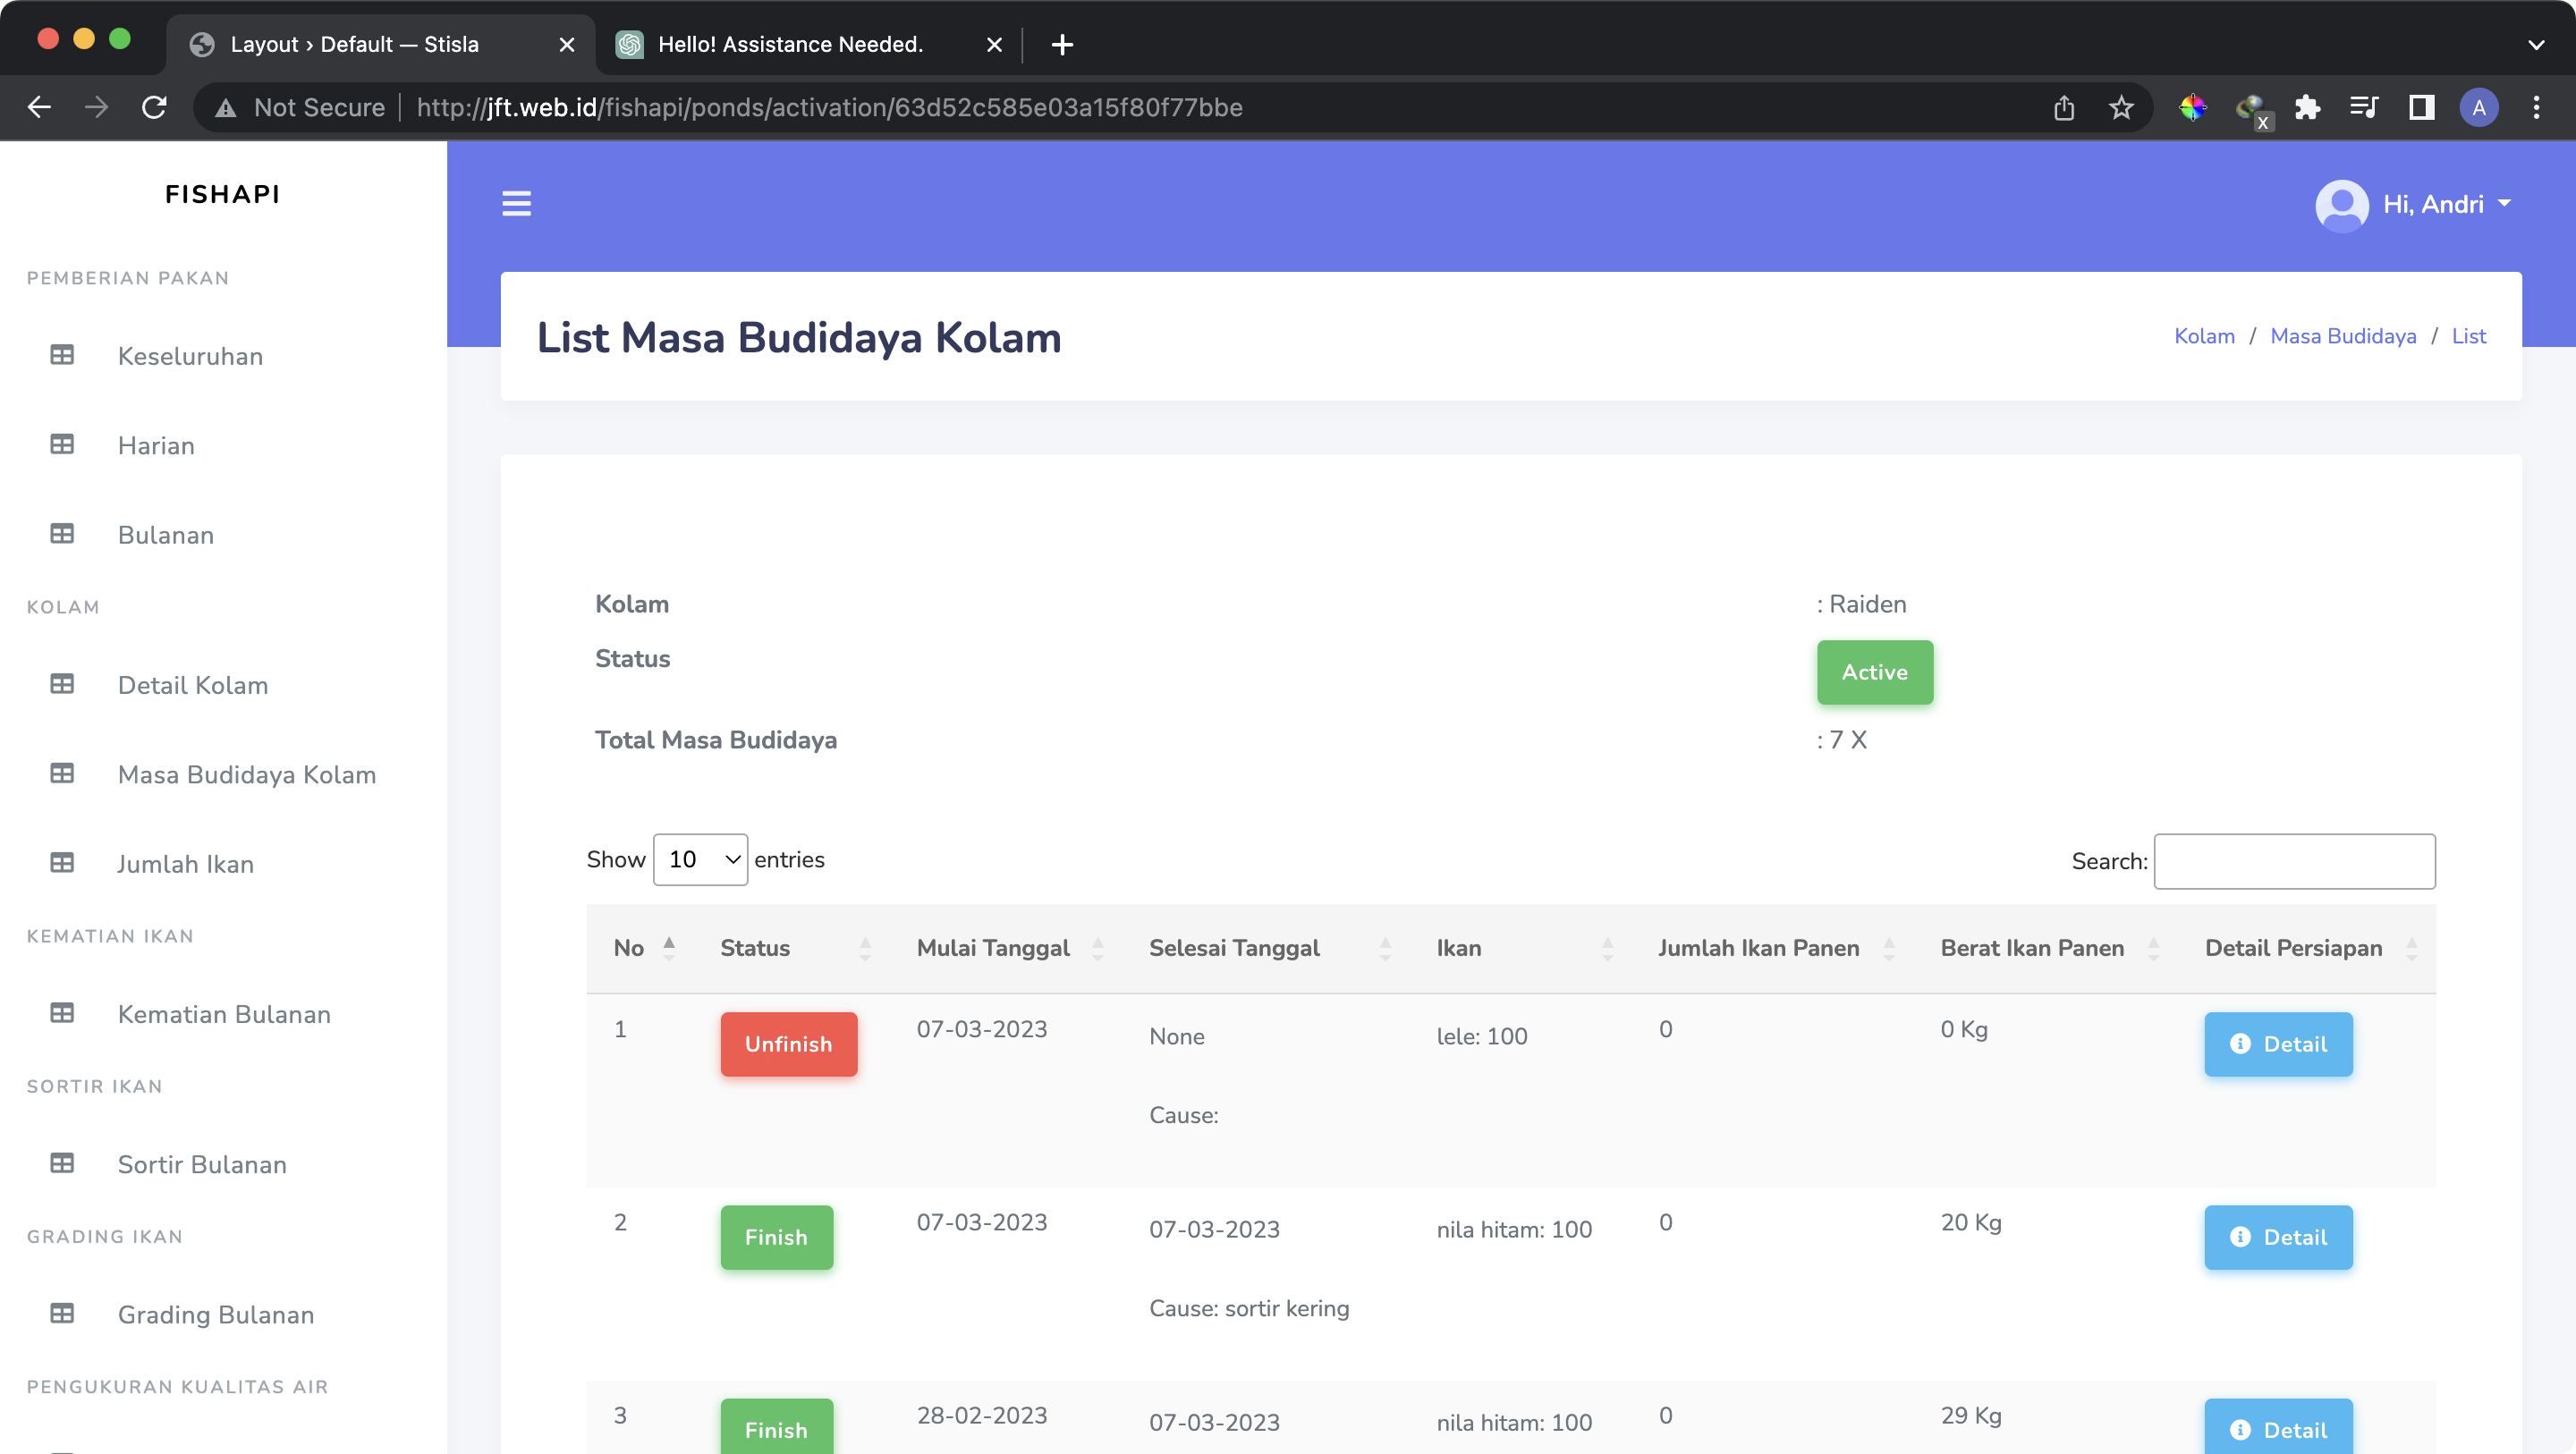
\includegraphics[width=1\textwidth]{gambar/Sprint04/view/view_list_musim_budidaya_perkolam}
	\caption{View list musim budidaya per kolam}
	\label{fig:view_list_musim_budidaya_perkolam}
\end{figure}


\item \textbf{Membuat view detail budidaya}
\begin{figure}[H]
	\centering
	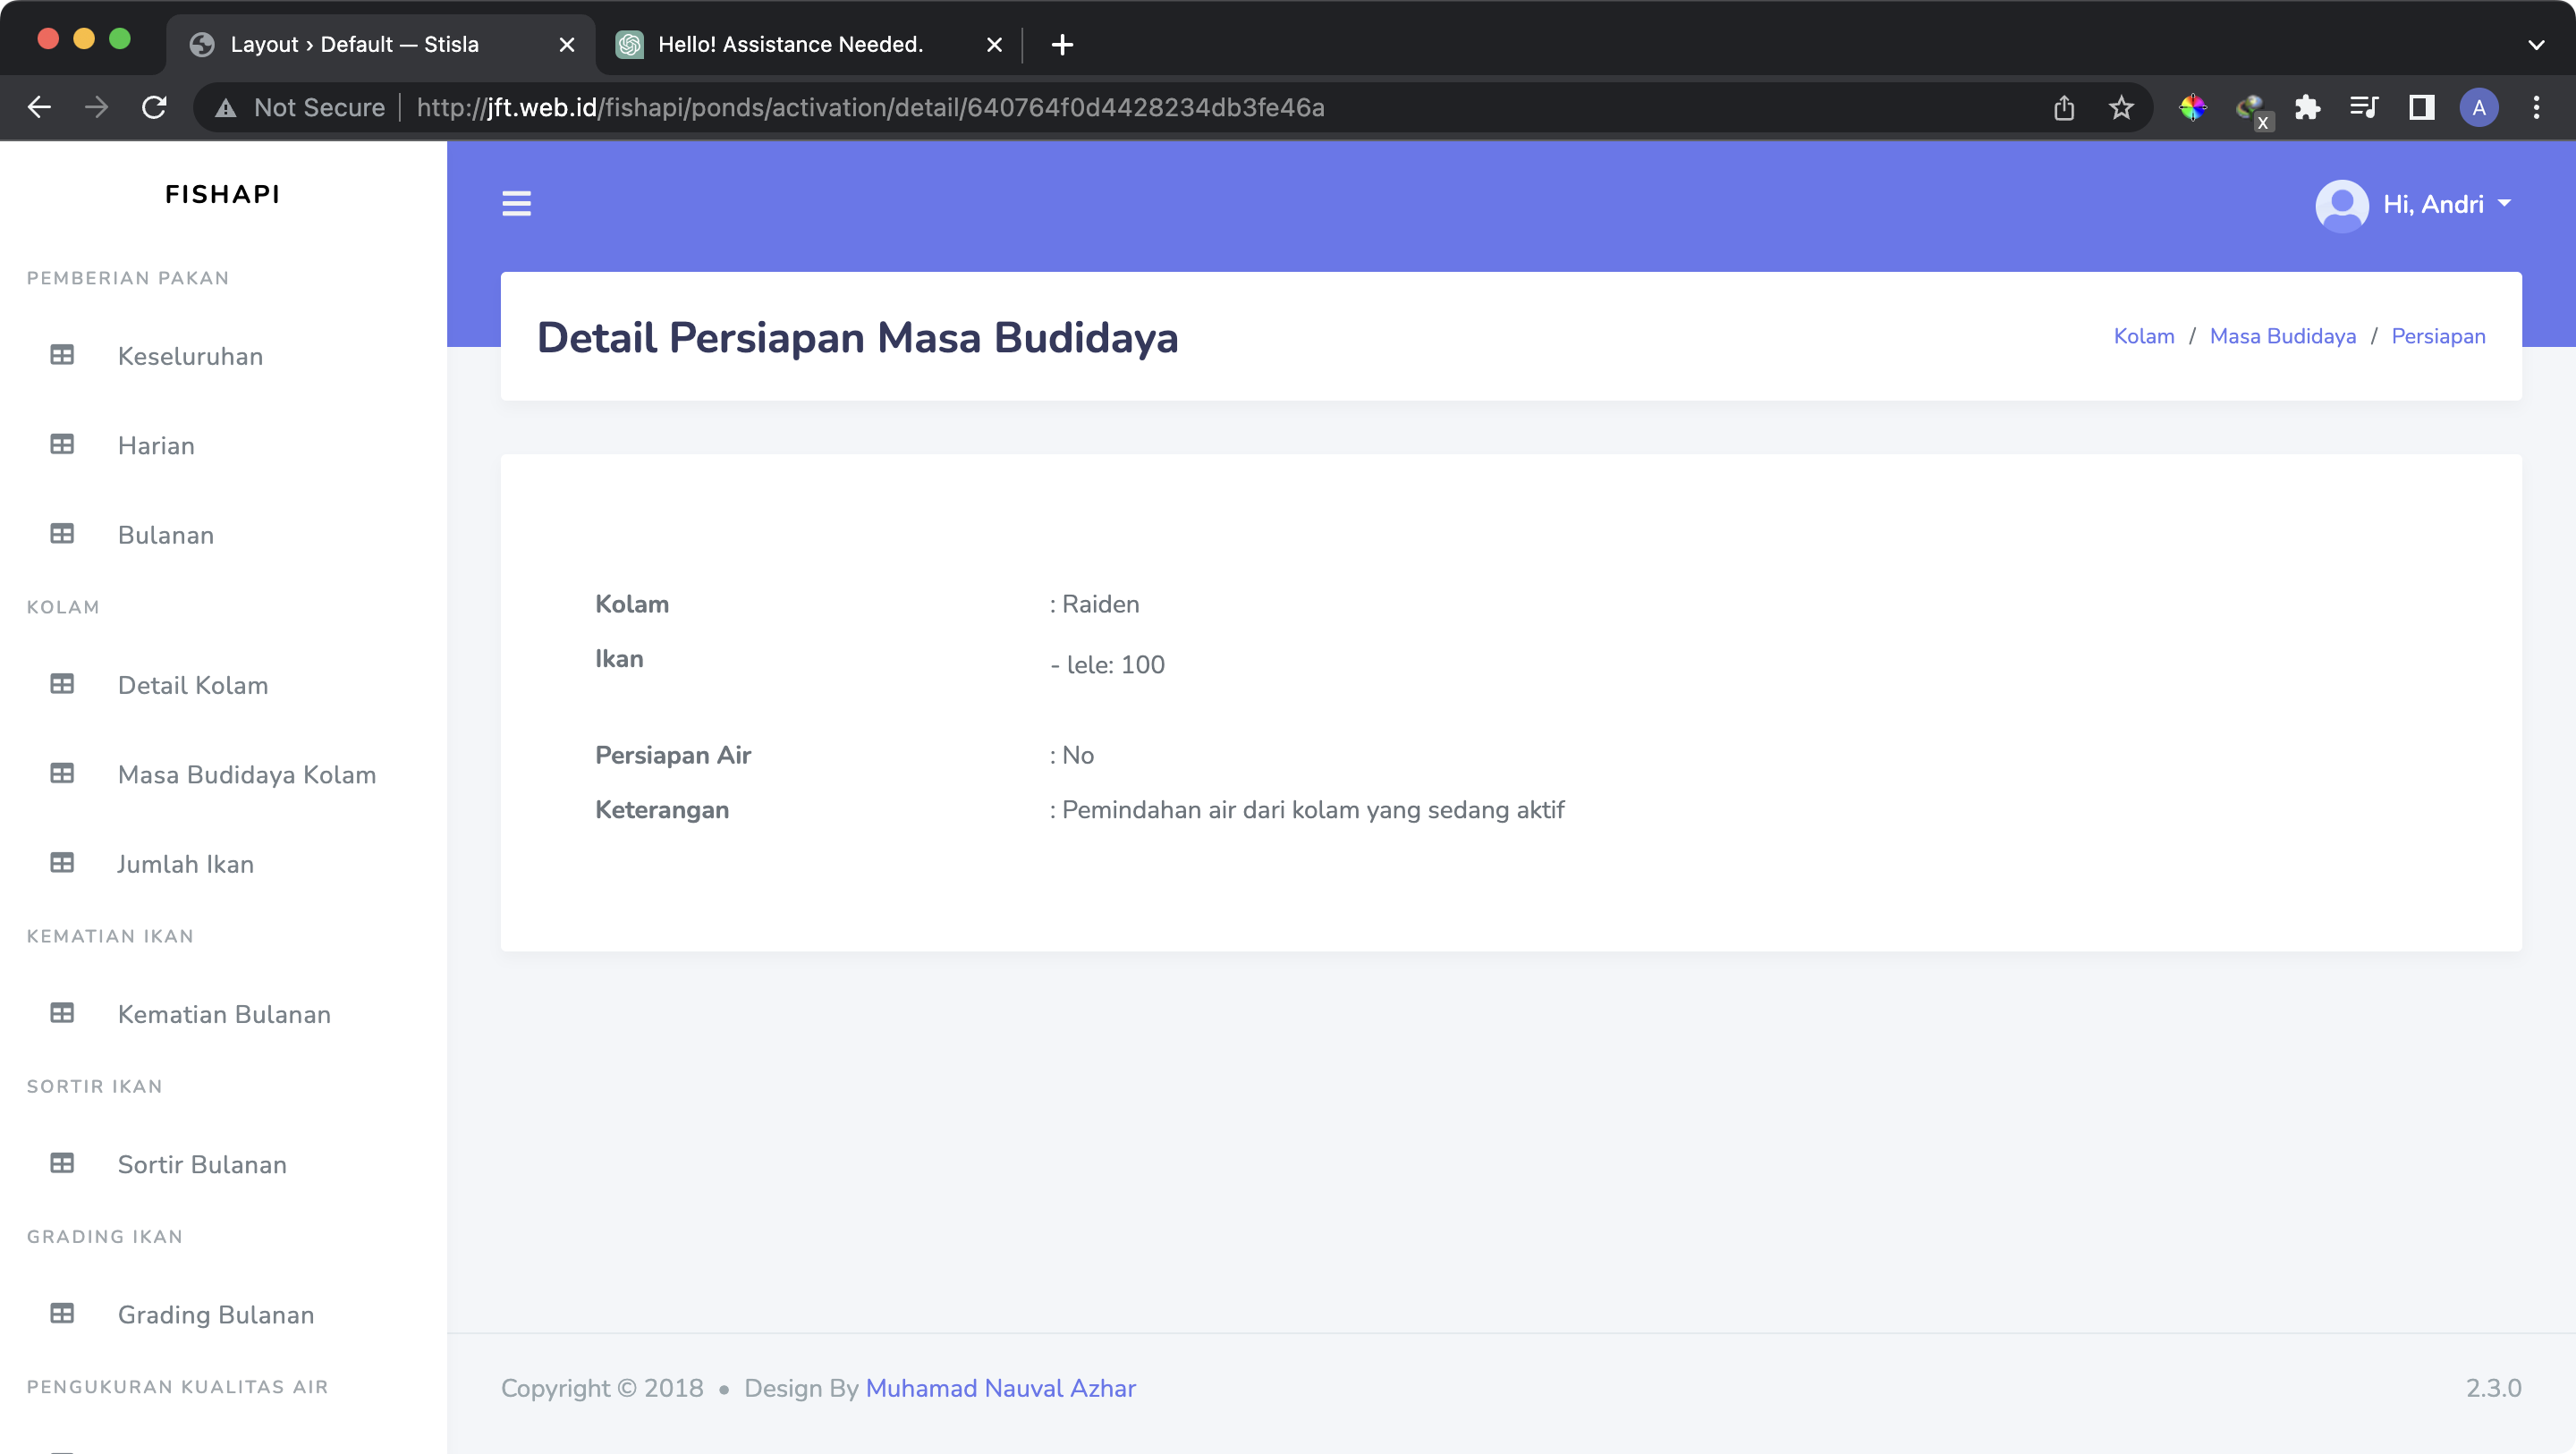
\includegraphics[width=1\textwidth]{gambar/Sprint04/view/view_detail_budidaya}
	\caption{View detail musim budidaya}
	\label{fig:view_detail_budidaya}
\end{figure}



\end{enumerate}
%!TEX root = ./template-skripsi.tex

\subsection{Sprint 5 Report}
Berikut merupakan report dari sprint ke-5 yang dilakukan pada tanggal 22 juni - 28 juni 2022.

\begin{table}[H]
	\caption{\textit{Sprint-5 backlog}}
	\label{sprint5_backlog}
	\begin{tabular}{@{} |p{0.5cm}|p{5cm}|p{5cm}|p{2cm}| @{}}
		\hline
		\textbf{No} & \textbf{\textit{Story}} & \textbf{\textit{Task}} & \textbf{\textit{Status}} \\
		\hline
		1 & \multirow{3}{5cm}{Create, Read, Updte, dan Delete untuk Pencatatan data kematian ikan} & Membarui desain database  & Completed\\
		\cline{1-1}\cline{3-4}
		2 & & Implementasi controller entry kematian ikan & Completed\\
		\cline{1-1}\cline{3-4}
		3 & & Implementasi controller edit kematian ikan & Completed\\
		\cline{1-1}\cline{3-4}
		4 & & Implementasi controller fetch list kematian ikan berdasarkan kolam & Next Spirnt\\
		\cline{1-1}\cline{3-4}
		5 & & Membuat view rekap kematian ikan perbulan & Next Sprint\\
		\cline{1-1}\cline{3-4}
		\hline
	\end{tabular}
\end{table}

\begin{enumerate}[1.]

\item \textbf{Membarui desain database}

\begin{figure}[H]
	\centering
	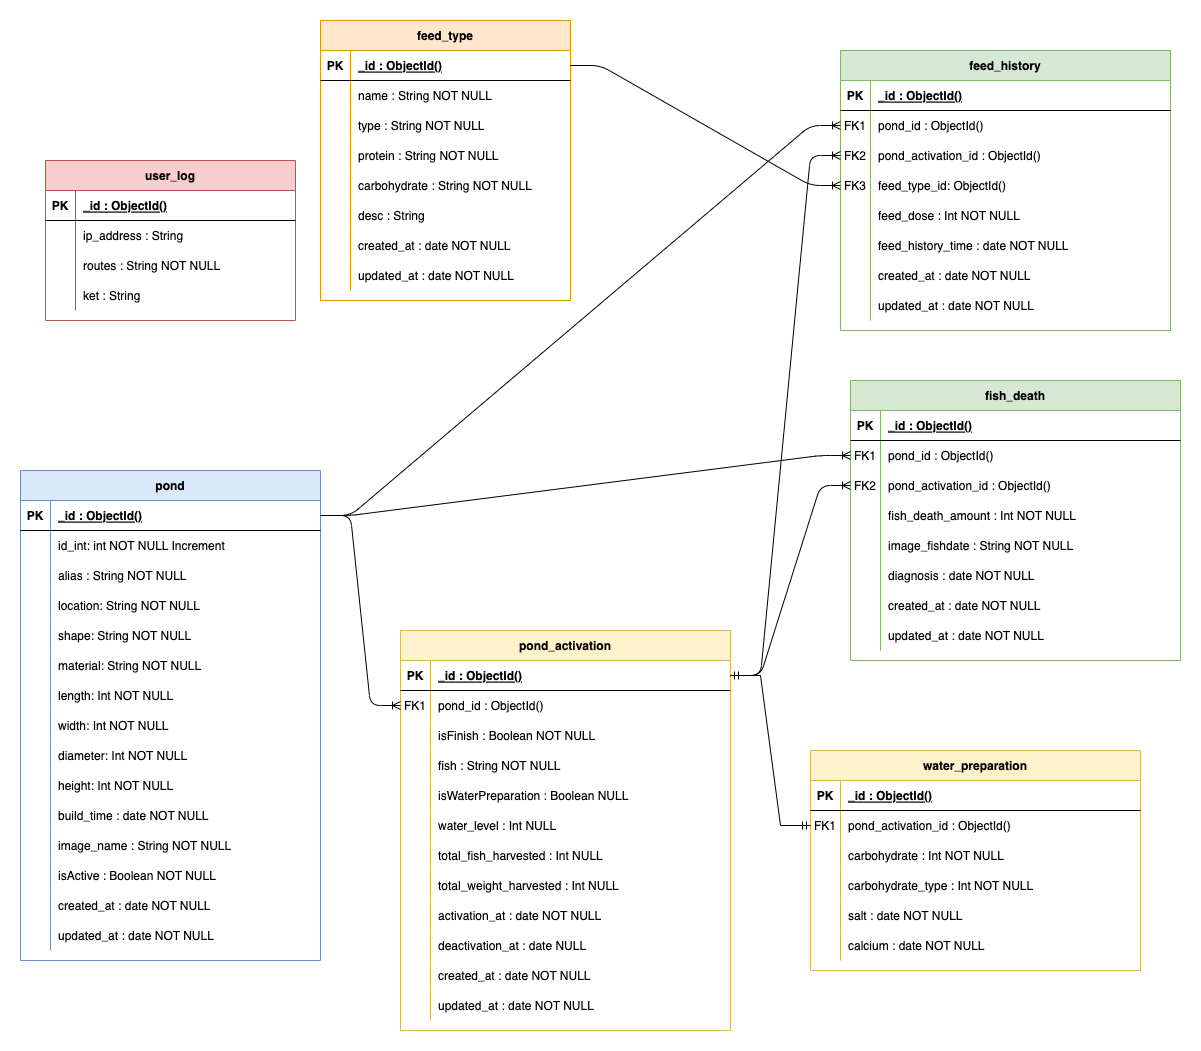
\includegraphics[height=0.7\textwidth]{gambar/Sprint05/diagram database/database}
	\caption{ERD Database Sprint-5}
	\label{fig:database_sprint5}
\end{figure}

Dengan berubahnya desain database diperlukan juga penambahan model pada source code, berikut perubahan pada source code model.

\begin{lstlisting}
# fishapi/database/model.py

class FishDeath(db.Document):
    pond_id = db.ReferenceField(Pond, required=True)
    pond_activation_id = db.ReferenceField(PondActivation, required=True)
    image_name = db.StringField(required=True)
    diagnosis = db.StringField(default=datetime.datetime.now)
    death_at = db.DateTimeField(default=datetime.datetime.now)
    created_at = db.DateTimeField(default=datetime.datetime.now)
    updated_at = db.DateTimeField(default=datetime.datetime.now)
\end{lstlisting}




\item \textbf{Implementasi API entry kematian ikan}

Implementasi controller API entry kematian ikan, berikut merupakan perubahan source code controller API entry kematian ikan.

\begin{lstlisting}
# fishapi/database/fishdeath.py

class PondActivationApi(Resource):
    def post(self):
        try:
            pond_id = request.form.get("pond_id", None)
            pond = Pond.objects.get(id=pond_id)
            if pond.isActive == False:
                response = {"message": "status pond is not active"}
                response = json.dumps(response, default=str)
                return Response(response, mimetype="application/json", status=400)
            pond_activation = PondActivation.objects(
                pond_id=pond_id, isFinish=False).order_by('-activated_at').first()
            try:
                file = request.files['image', None]
                if not allowed_file(file.filename):
                    response = {"message": "file type not allowed"}
                    response = json.dumps(response, default=str)
                    return Response(response, mimetype="application/json", status=400)
                filename = secure_filename(file.filename)
                filename = pad_timestamp(filename)
                path = os.path.join(current_app.instance_path,
                                    current_app.config['UPLOAD_DIR'])
                try:
                    os.makedirs(path)
                except OSError:
                    pass
                filepath = os.path.join(path, filename)
                file.save(filepath)
            except:
                filename = "default.jpg"
            fish_death_amount = request.form.get("fish_death_amount", "[]")
            fish_death_amount = json.loads(fish_death_amount)
            if len(fish_death_amount) < 1:
                response = {"message": "There is no fish"}
                response = json.dumps(response, default=str)
                return Response(response, mimetype="application/json", status=400)
            body = {
                "pond_id": pond.id,
                "pond_activation_id": pond_activation.id,
                "image_name": filename,
                "diagnosis": request.form.get("diagnosis", None),
            }
            fishdeath = FishDeath(**body).save()
            id = fishdeath.id
            for fish in fish_death_amount:
                # save fish log
                data = {
                    "pond_id": pond_id,
                    "pond_activation_id": pond_activation.id,
                    "fish_death_id": id,
                    "type_log": "death",
                    "fish_type": fish['type'],
                    "fish_amount": int(fish['amount']) * -1
                }
                fishlog = FishLog(**data).save()
            response = {"message": "success add fishdeath"}
            response = json.dumps(response, default=str)
            return Response(response, mimetype="application/json", status=200)
        except Exception as e:
            response = {"message": str(e)}
            response = json.dumps(response, default=str)
            return Response(response, mimetype="application/json", status=400)
\end{lstlisting}

Kode ini adalah sebuah fungsi yang menangani permintaan POST yang dikirimkan ke server.

Pertama, fungsi ini mencoba untuk mengambil nilai "pond\_id" dari permintaan yang diterima. Jika nilai ini tidak ada, maka nilai "pond\_id" akan diatur menjadi None. Kemudian fungsi mencoba untuk mendapatkan objek Pond dari database dengan menggunakan nilai "pond\_id" yang diperoleh sebelumnya.

Jika nilai isActive dari objek Pond adalah False, maka fungsi akan mengembalikan pesan kesalahan dengan kode status 400. Jika nilai isActive adalah True, maka fungsi akan mencoba mendapatkan objek PondActivation dengan menggunakan nilai "pond\_id" yang diperoleh sebelumnya. Objek PondActivation yang diperoleh akan memiliki isFinish=False dan diurutkan berdasarkan tanggal aktivasi terbaru.

Selanjutnya, fungsi akan mencoba untuk mendapatkan file gambar dari permintaan yang diterima. Jika jenis file tidak diizinkan, maka fungsi akan mengembalikan pesan kesalahan dengan kode status 400. Jika jenis file diizinkan, maka fungsi akan menyimpan file gambar di dalam direktori yang ditentukan.

Setelah itu, fungsi akan mencoba untuk mengambil nilai "fish\_death\_amount" dari permintaan yang diterima dan mengonversinya menjadi objek Python. Jika nilai "fish\_death\_amount" kosong, maka fungsi akan mengembalikan pesan kesalahan dengan kode status 400.

Kemudian, fungsi akan membuat objek FishDeath dengan menggunakan nilai-nilai yang diperoleh sebelumnya, dan menyimpannya ke dalam database. Fungsi juga akan membuat objek FishLog untuk setiap jenis ikan yang tercatat mati, dan menyimpannya ke dalam database.

Terakhir, fungsi akan mengembalikan pesan sukses dengan kode status 200, atau pesan kesalahan dengan kode status 400 jika terjadi kesalahan selama proses. Semua pesan yang dikirimkan dalam format JSON.

Terakhir, fungsi mengembalikan respons dalam format JSON yang berisi pesan berhasil atau gagalnya aktivasi kolam.

Berikut merupakan form untuk entry musim budidaya.

\begin{longtable}{| l | p{5cm} | p{5cm} |}
\caption{Form entry kematian ikan.\label{table:form_entry_kematian_ikan}}\\

\hline
\multicolumn{1}{|c|}{\textbf{Form}} & \multicolumn{1}{|c|}{\textbf{Jenis Data}} & \multicolumn{1}{|c|}{\textbf{Deskripsi}}\\
\hline
\endfirsthead

\hline
\multicolumn{3}{|c|}{Lanjutan Tabel \ref{table:form_entry_kematian_ikan}}\\
\hline
\multicolumn{1}{|c|}{\textbf{Form}} & \multicolumn{1}{|c|}{\textbf{Jenis Data}} & \multicolumn{1}{|c|}{\textbf{Deskripsi}}\\
\hline
\endhead

                                          

pond\_id            & REQUIRED STRING                                                                                                                                             & id kolam yang mengalami kematian ikan \\ \hline
fish\_death\_amount & REQUIRED JSON FISH TYPE: {[}"nila hitam", "nila merah", "lele", "patin", "mas",{]} Ex: {[}\{"type": "lele","amount": 5\},\{"type": "patin","amount": 9\}{]} & tipe dan banyak ikan                  \\ \hline
image               & OPTIONAL FILE                                                                                                                                               & foto kematian ikan                    \\ \hline
diagnosis           & REQUIRED STRING                                                                                                                                             & diagnosa kematian ikan                \\ \hline

\end{longtable}


Tabel tersebut merupakan deskripsi dari jenis data yang diperlukan pada form untuk menambahkan data kematian ikan pada suatu kolam. Form ini meminta input berupa pond\_id yang merupakan string yang mengacu pada id kolam yang mengalami kematian ikan. Selain itu, input fish\_death\_amount juga diperlukan dalam bentuk JSON dengan jenis data yang terdiri dari "nila hitam", "nila merah", "lele", "patin", dan "mas". Fish\_death\_amount menyimpan informasi tentang jenis dan banyaknya ikan yang mati. Input file image bersifat opsional dan meminta foto kematian ikan, sedangkan diagnosis yang diperlukan dalam bentuk string merujuk pada diagnosa kematian ikan.

Berikut merupakan hasil test request dari API entry kematian ikan.

cURL:

\begin{lstlisting}
curl --location 'http://jft.web.id/fishapi/api/fishdeath' \
--form 'pond_id="625d7026a9a73e090c65cda1"' \
--form 'fish_death_amount="[{\"lele\": 10},{\"patin\":20}]"' \
--form 'image=@"/Users/andrirahmanto/Downloads/Mass-fish-death-Menindee.jpeg"' \
--form 'diagnosis="mati karena sakit"'
\end{lstlisting}

response json:

\begin{lstlisting}
{
  "message": "success add fishdeath",
  "id": "62b9adfa793e0f39dbaa1739"
}
\end{lstlisting}




\item \textbf{Implementasi API edit kematian ikan}

Implementasi controller API edit kematian ikan, berikut merupakan perubahan source code controller API edit kematian ikan.

\begin{lstlisting}
# fishapi/database/fishdeath.py

def put(self, id):
        try:
            body = request.form.to_dict(flat=True)
            FishDeath.objects.get(id=id).update(**body)
            response = {"message": "success change data fish death", "id": id}
            response = json.dumps(response, default=str)
            return Response(response, mimetype="application/json", status=200)
        except Exception as e:
            response = {"message": str(e)}
            response = json.dumps(response, default=str)
            return Response(response, mimetype="application/json", status=400)
        return
\end{lstlisting}

Kode ini merupakan fungsi untuk mengubah data kematian ikan pada database. Fungsi ini menggunakan HTTP method PUT dan menerima parameter id, yang merupakan id dari data kematian ikan yang ingin diubah.

Pada blok try, terdapat dua baris kode. Baris pertama mengubah data request.form menjadi dictionary yang disimpan dalam variabel body. Baris kedua memanggil fungsi update pada model FishDeath dengan mengirimkan id dan dictionary body sebagai parameter.

Jika proses berhasil, akan mengembalikan response dengan status 200 dan message "success change data fish death" beserta id dari data yang diubah. Jika terjadi error, maka akan mengembalikan response dengan status 400 dan message error yang muncul pada variabel e yang diubah menjadi string.

Blok terakhir menggunakan return untuk mengakhiri fungsi.

Berikut merupakan form untuk edit kematian ikan.

\begin{longtable}{| l | p{5cm} | p{5cm} |}
\caption{Form edit kematian ikan.\label{table:form_edit_kematian_ikan}}\\

\hline
\multicolumn{1}{|c|}{\textbf{Form}} & \multicolumn{1}{|c|}{\textbf{Jenis Data}} & \multicolumn{1}{|c|}{\textbf{Deskripsi}}\\
\hline
\endfirsthead

\hline
\multicolumn{3}{|c|}{Lanjutan Tabel \ref{table:form_edit_kematian_ikan}}\\
\hline
\multicolumn{1}{|c|}{\textbf{Form}} & \multicolumn{1}{|c|}{\textbf{Jenis Data}} & \multicolumn{1}{|c|}{\textbf{Deskripsi}}\\
\hline
\endhead

                                          

pond\_id            & REQUIRED STRING                                                                                                                                             & id kolam yang mengalami kematian ikan \\ \hline
fish\_death\_amount & OPTIONAL JSON FISH TYPE: {[}"nila hitam", "nila merah", "lele", "patin", "mas",{]} Ex: {[}\{"type": "lele","amount": 5\},\{"type": "patin","amount": 9\}{]} & tipe dan banyak ikan                  \\ \hline
diagnosis           & OPTIONAL STRING                                                                                                                                             & diagnosa kematian ikan                \\ \hline

\end{longtable}


Tabel ini adalah deskripsi dari form edit kematian ikan dan memiliki tiga kolom yaitu Form, Jenis Data, dan Deskripsi.

Form menjelaskan nama dari field input pada form, Jenis Data menjelaskan tipe data dari field input, sedangkan Deskripsi memberikan penjelasan singkat mengenai deskripsi dari field input tersebut.

Pada tabel ini, terdapat 3 field input yaitu pond\_id, fish\_death\_amount, dan diagnosis. Kolom Jenis Data menunjukkan apakah field input tersebut merupakan tipe data REQUIRED STRING atau OPTIONAL JSON FISH TYPE dan Deskripsi memberikan penjelasan mengenai field input tersebut.

Field pond\_id wajib diisi dan berisi id kolam yang mengalami kematian ikan, sedangkan field fish\_death\_amount dan diagnosis bersifat opsional. Field fish\_death\_amount berisi tipe dan banyak ikan yang mati dan ditulis dalam format JSON, sedangkan field diagnosis berisi diagnosa kematian ikan.
Berikut merupakan hasil test request dari API entry kematian ikan.

cURL:

\begin{lstlisting}
curl --location -g --request PUT 'http://jft.web.id/fishapi/api/fishdeath/{fishdeath_id}' \
--form 'fish_death_amount="[{\"lele\": 10},{\"patin\":20}]"' \
--form 'diagnosis="mati karena sakit"'
\end{lstlisting}

response json:

\begin{lstlisting}
{
  "message": "success change data fish death",
  "id": "62b9adfa793e0f39dbaa1739"
}
\end{lstlisting}









\end{enumerate}
%!TEX root = ./template-skripsi.tex

\subsection{Sprint 6 Report}
Berikut merupakan report dari sprint ke-5 yang dilakukan pada tanggal 29 juni - 5 juli 2022.

\begin{table}[H]
	\caption{\textit{Sprint-6 backlog}}
	\label{sprint6_backlog}
	\begin{tabular}{@{} |p{0.5cm}|p{5cm}|p{5cm}|p{2cm}| @{}}
		\hline
		\textbf{No} & \textbf{\textit{Story}} & \textbf{\textit{Task}} & \textbf{\textit{Status}} \\
		\hline
		1 & & Implementasi controller delete kematian ikan & Complete\\
		\cline{1-1}\cline{3-4}
		2 & & Membuat view rekap kematian ikan perbulan & Complete\\
		\cline{1-1}\cline{3-4}
		\hline
	\end{tabular}
\end{table}

\begin{enumerate}[1.]



\item \textbf{Implementasi API fetch list kematian ikan berdasarkan kolam}

Implementasi controller API fetch list kematian ikan berdasarkan kolam, berikut merupakan source code controller API fetch list kematian ikan berdasarkan kolam.

\begin{lstlisting}
# fishapi/database/fishdeath.py

def get(self):
        try:
            url = url_for('fishdeathimageapidummy', _external=True)
            pipeline = [
                {'$lookup': {
                    'from': 'pond_activation',
                    'let': {"pondid": "$_id"},
                    'pipeline': [
                        {'$match': {'$expr': {'$and': [
                            {'$eq': ['$pond_id', '$$pondid']},
                            {'$eq': ['$isFinish', False]},
                        ]}}},
                        {"$lookup": {
                            "from": "fish_death",
                            "let": {"activationid": "$_id"},
                            "pipeline": [
                                {'$match': {'$expr': {'$and': [
                                    {'$eq': ['$pond_activation_id',
                                             '$$activationid']},
                                ]}}},
                                {'$lookup': {
                                    'from': 'fish_log',
                                    'let': {"fish_death_id": "$_id"},
                                    'pipeline': [
                                        {'$match': {
                                            '$expr': {'$and': [
                                                {'$eq': ['$fish_death_id',
                                                         '$$fish_death_id']},
                                                {'$eq': ['$type_log',
                                                         'death']},
                                            ]}
                                        }},
                                        {"$project": {
                                            "created_at": 0,
                                            "updated_at": 0,
                                        }}
                                    ],
                                    'as': 'fish'
                                }},
                                {"$addFields": {
                                    "image_link": {"$concat": [url, "/", {"$toString": "$_id"}]}
                                }},
                                {"$project": {
                                    "pond_id": 0,
                                    "pond_activation_id": 0,
                                    "created_at": 0,
                                    "updated_at": 0,
                                }}
                            ],
                            "as": "fish_death_list",
                        }},
                        {"$project": {
                            "pond_id": 0,
                            "feed_type_id": 0,
                            "created_at": 0,
                            "updated_at": 0,
                        }}
                    ],
                    'as': 'pond_activation_list'
                }},
                {"$addFields": {
                    "pond_activation": {"$first": "$pond_activation_list"},
                }},
                {"$project": {
                    "location": 0,
                    "shape": 0,
                    "material": 0,
                    "length": 0,
                    "width": 0,
                    "diameter": 0,
                    "height": 0,
                    "image_name": 0,
                    "pond_activation_list": 0,
                    "updated_at": 0,
                    "created_at": 0,
                }}
            ]
            ponds = Pond.objects.aggregate(pipeline)
            list_ponds = list(ponds)
            response = json.dumps(list_ponds, default=str)
            return Response(response, mimetype="application/json", status=200)
        except Exception as e:
            response = {"message": str(e)}
            response = json.dumps(response, default=str)
            return Response(response, mimetype="application/json", status=400)
\end{lstlisting}

Kode yang diberikan adalah sebuah method get yang ada di dalam sebuah class. Method ini menerima request GET untuk mengambil data dari MongoDB database.

Berikut adalah langkah-langkah yang dilakukan oleh method get:

\begin{enumerate}[a.]
\item Membuat URL dari fishdeathimageapidummy dengan menggunakan url\_for dan menyimpannya ke dalam variabel url.
\item Membuat sebuah pipeline untuk melakukan aggregate query pada collection Pond.
\item Pada pipeline tersebut, melakukan lookup terhadap collection pond\_activation dengan menggunakan field \_id dari collection Pond sebagai input.
\item Pada hasil lookup pertama, mencocokkan nilai dari field isFinish yang bernilai False.
\item Pada hasil lookup kedua, mencocokkan nilai dari field pond\_activation\_id yang sama dengan \_id dari hasil lookup pertama.
\item Pada hasil lookup ketiga, mencocokkan nilai dari field fish\_death\_id yang sama dengan \_id dari hasil lookup kedua dan type\_log yang bernilai death.
\item Melakukan projeksi untuk mengambil field-field tertentu yang dibutuhkan dan mengecualikan beberapa field yang tidak dibutuhkan.
\item Menyimpan hasil query dalam variabel ponds.
\item Mengubah hasil query menjadi sebuah list dan mengubahnya menjadi JSON dengan menggunakan json.dumps.
\item Membungkus hasil JSON kedalam sebuah response dengan menggunakan Response.
\item Jika terdapat exception, maka akan membuat sebuah response dengan pesan error dan mengembalikan response tersebut.
\item Inti dari kode ini adalah melakukan sebuah aggregate query pada collection Pond dengan menggunakan beberapa lookup dan projeksi untuk mengambil data yang dibutuhkan dan menyajikan hasil query dalam bentuk JSON.
\end{enumerate}


Berikut merupakan hasil test request dari API get list kematian ikan.

cURL:

\begin{lstlisting}
curl --location 'http://jft.web.id/fishapi/api/fishdeath'
\end{lstlisting}

response json:

\begin{lstlisting}
[
  {
    "_id": "62a62163e445ffb9c5f746f3",
    "id_int": 4,
    "alias": "charlie",
    "build_at": "2022-06-13 00:24:51.473000",
    "isActive": false
  },
  {
    "_id": "625d7033a9a73e090c65cda2",
    "id_int": 3,
    "alias": "beta",
    "build_at": "2022-04-18 21:05:39.608000",
    "isActive": true,
    "pond_activation": {
      "_id": "62b6b2f1a8a50041ee6350a4",
      "isFinish": false,
      "fish": [
        {
          "lele": 100
        },
        {
          "patin": 200
        }
      ],
      "isWaterPreparation": false,
      "water_level": 100,
      "total_fish_harvested": 0,
      "total_weight_harvested": 0,
      "activated_at": "2022-06-25 14:02:09.881000",
      "fish_death_list": []
    }
  },
  {
    "_id": "625d7026a9a73e090c65cda1",
    "id_int": 2,
    "alias": "alpha",
    "build_at": "2022-04-18 21:05:26.183000",
    "isActive": true,
    "pond_activation": {
      "_id": "62af4c24f6a3ffba25a6be6a",
      "isFinish": false,
      "fish": [
        {
          "lele": 100
        },
        {
          "patin": 200
        }
      ],
      "isWaterPreparation": false,
      "water_level": 1.34,
      "total_fish_harvested": 0,
      "total_weight_harvested": 0,
      "activated_at": "2022-06-19 23:17:40.501000",
      "fish_death_list": [
        {
          "_id": "62b9adfa793e0f39dbaa1739",
          "fish_death_amount": [
            {
              "lele": 10
            },
            {
              "patin": 20
            }
          ],
          "image_name": "Mass-fish-death-Menindee_1656335866.jpeg",
          "diagnosis": "mati karena sakit",
          "image_link": "http://127.0.0.1:5000/api/fishdeath/image/62b9adfa793e0f39dbaa1739"
        }
      ]
    }
  },
  {
    "_id": "62a955888911334402ddb3b3",
    "id_int": 5,
    "alias": "delta",
    "build_at": "2022-06-15 10:44:08.180000",
    "isActive": false
  },
  {
    "_id": "62ada3ff1dc3a711668e7ca3",
    "id_int": 7,
    "alias": "epsilon",
    "isActive": false,
    "build_at": "2022-06-18 17:07:59.396000"
  }
]
\end{lstlisting}

\item \textbf{Membuat view rekap kematian ikan perbulan}
\begin{figure}[H]
	\centering
	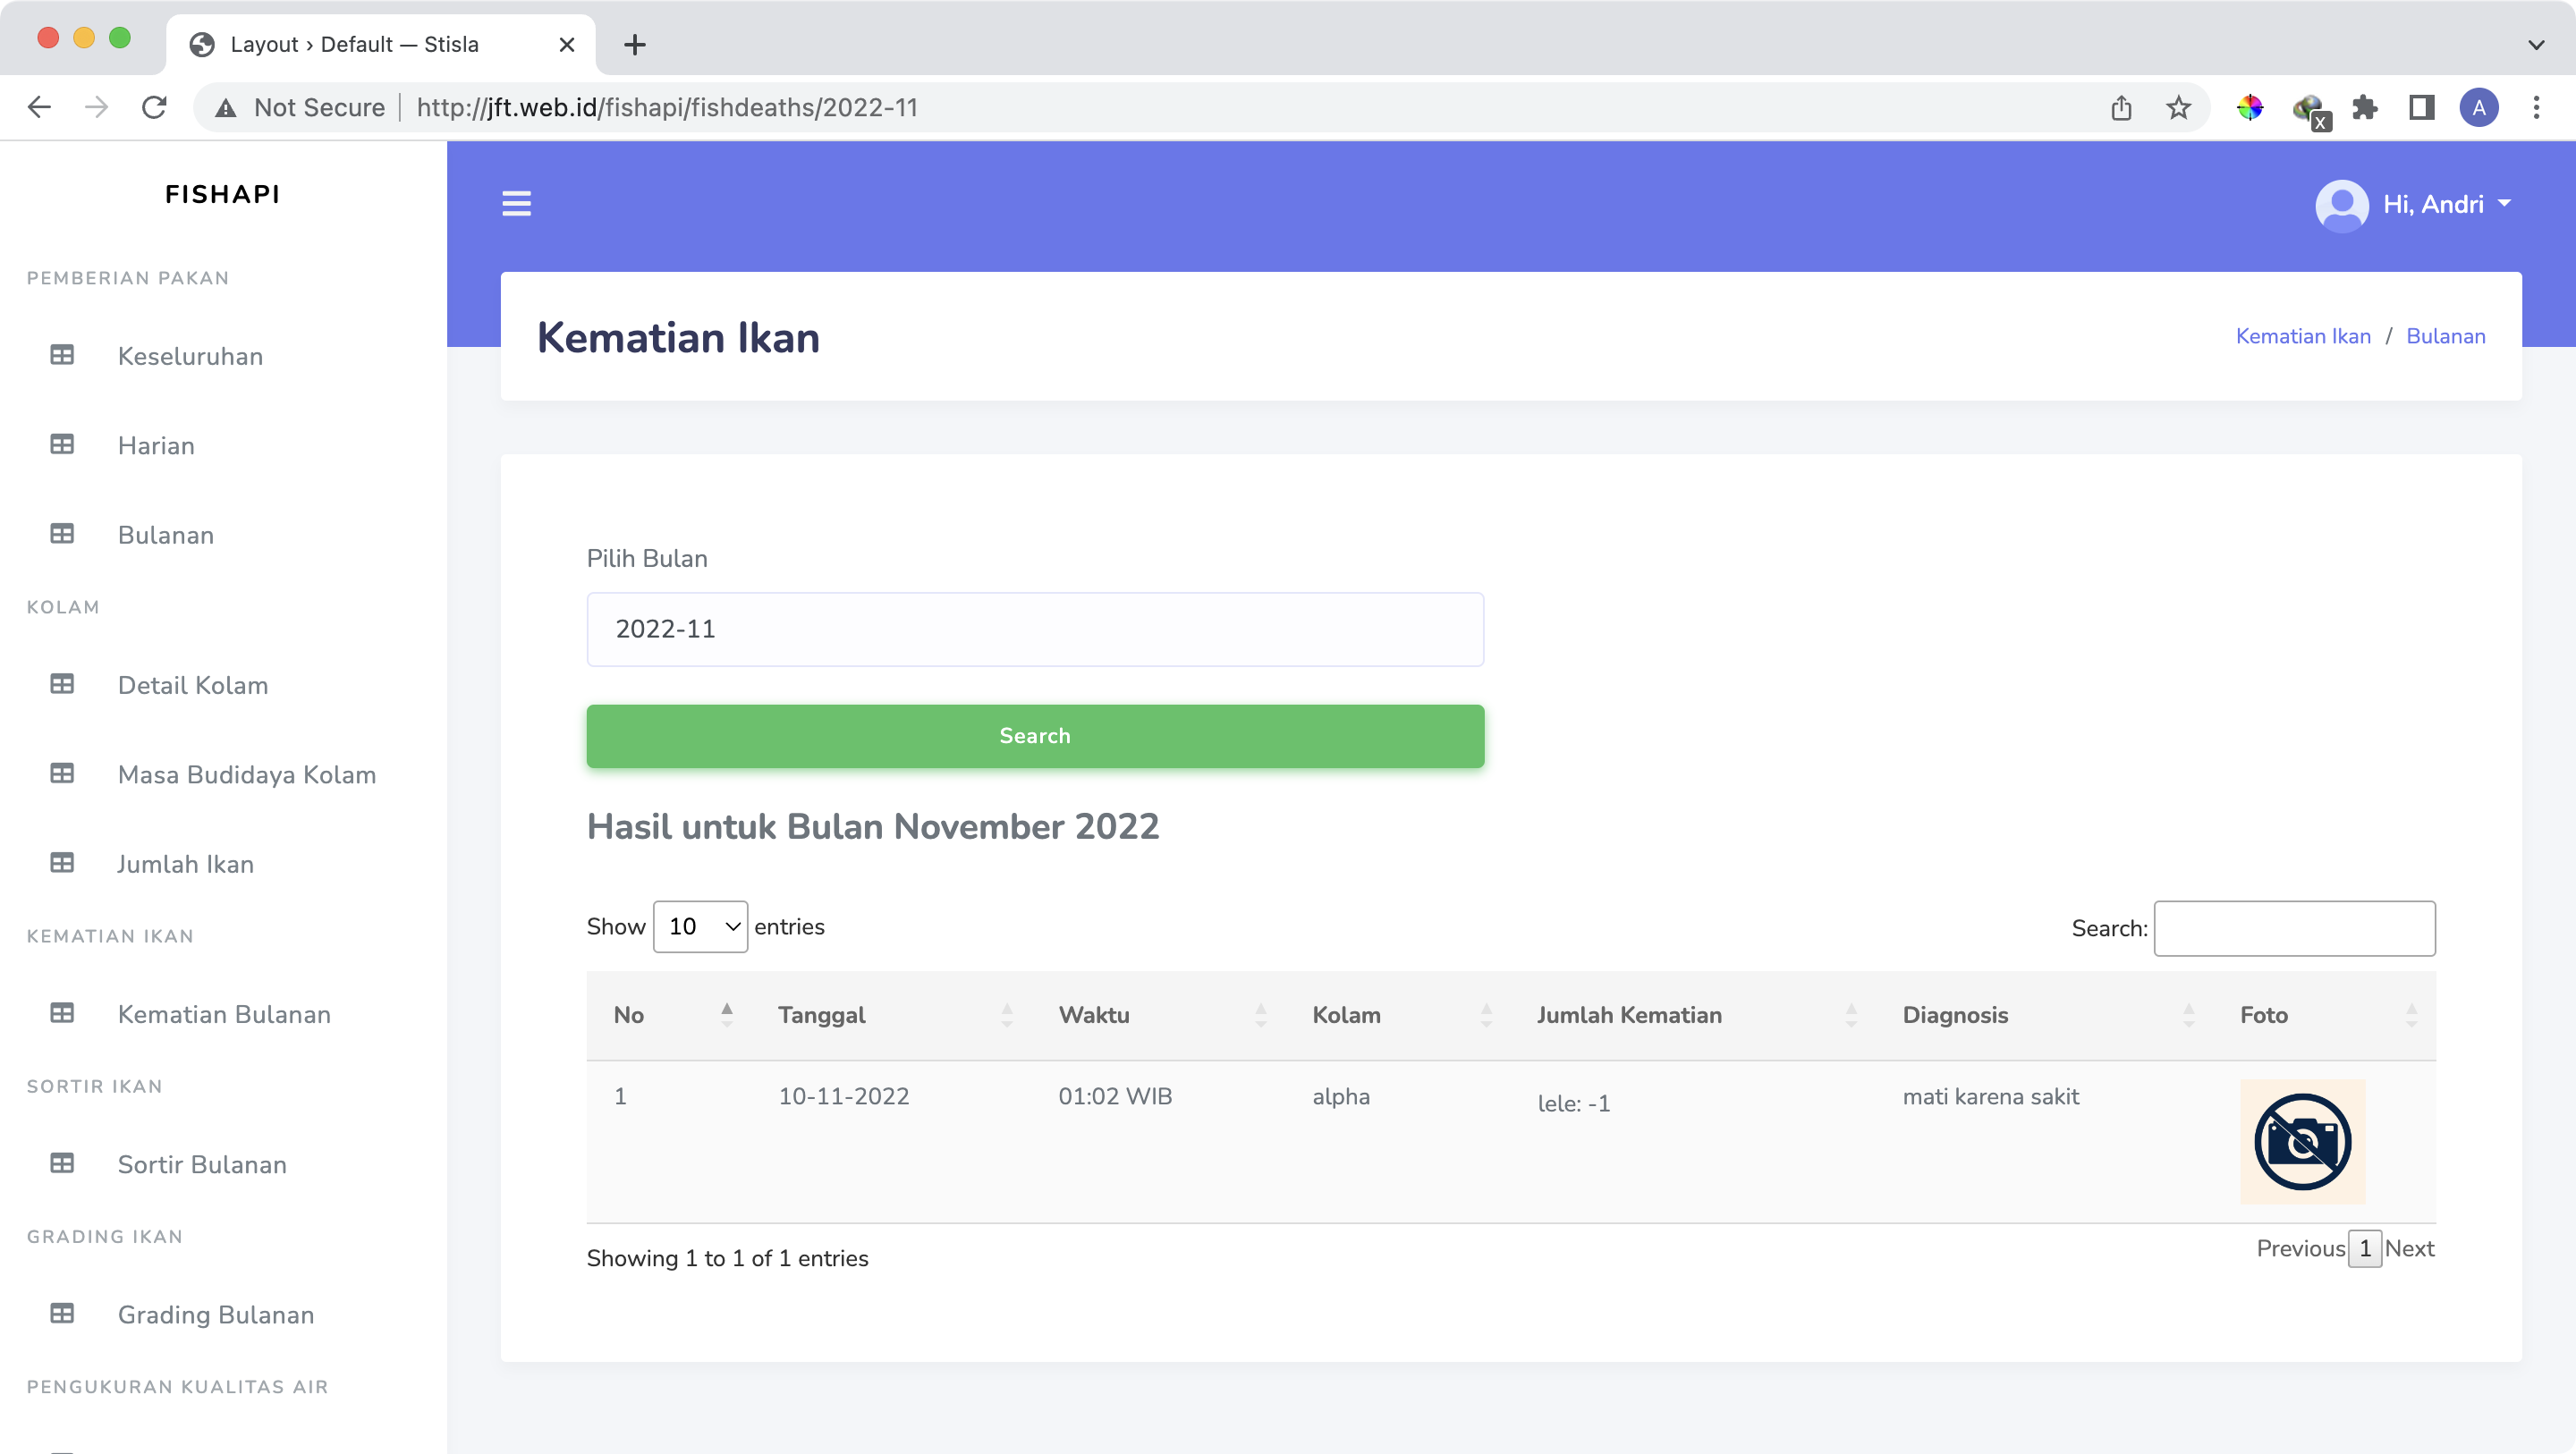
\includegraphics[width=1\textwidth]{gambar/Sprint05/view/view_kematian_bulanan}
	\caption{View list kematian perbulan}
	\label{fig:view_list_kematian_bulanan}
\end{figure}




\end{enumerate}
%!TEX root = ./template-skripsi.tex

\subsection{Sprint 7 Report}
Berikut merupakan report dari sprint ke-7 yang dilakukan pada tanggal 6 juni - 12 juni 2022.

\begin{table}[H]
	\caption{\textit{Sprint-7 backlog}}
	\label{sprint7_backlog}
	\begin{tabular}{@{} |p{0.5cm}|p{5cm}|p{5cm}|p{2cm}| @{}}
		\hline
		\textbf{No} & \textbf{\textit{Story}} & \textbf{\textit{Task}} & \textbf{\textit{Status}} \\
		\hline
		1 & \multirow{3}{5cm}{Create, Read, Updte, dan Delete untuk Pencatatan perpindahan ikan} & Membarui desain database  & Completed\\
		\cline{1-1}\cline{3-4}
		2 & & Menambahkan routes API & Completed\\
		\cline{1-1}\cline{3-4}
		3 & & Implementasi controller entry perpindahan ikan & Completed\\
		\cline{1-1}\cline{3-4}
		4 & & Implementasi controller fetch list perpindahan ikan & Completed\\
		\cline{1-1}\cline{3-4}
		5 & & Implementasi controller edit perpindahan ikan & Completed\\
		\cline{1-1}\cline{3-4}
		6 & & Implementasi controller delete perpindahan ikan & Completed\\
		\cline{1-1}\cline{3-4}
		7 & & Implementasi controller fetch perpindahan ikan dengan id& Completed\\
		\cline{1-1}\cline{3-4}
		8 & & Membuat view rekap perpindahan ikan & Completed\\
		\cline{1-1}\cline{3-4}
		\hline
	\end{tabular}
\end{table}

\begin{enumerate}[1.]

\item \textbf{Membarui desain database}

\begin{figure}[H]
	\centering
	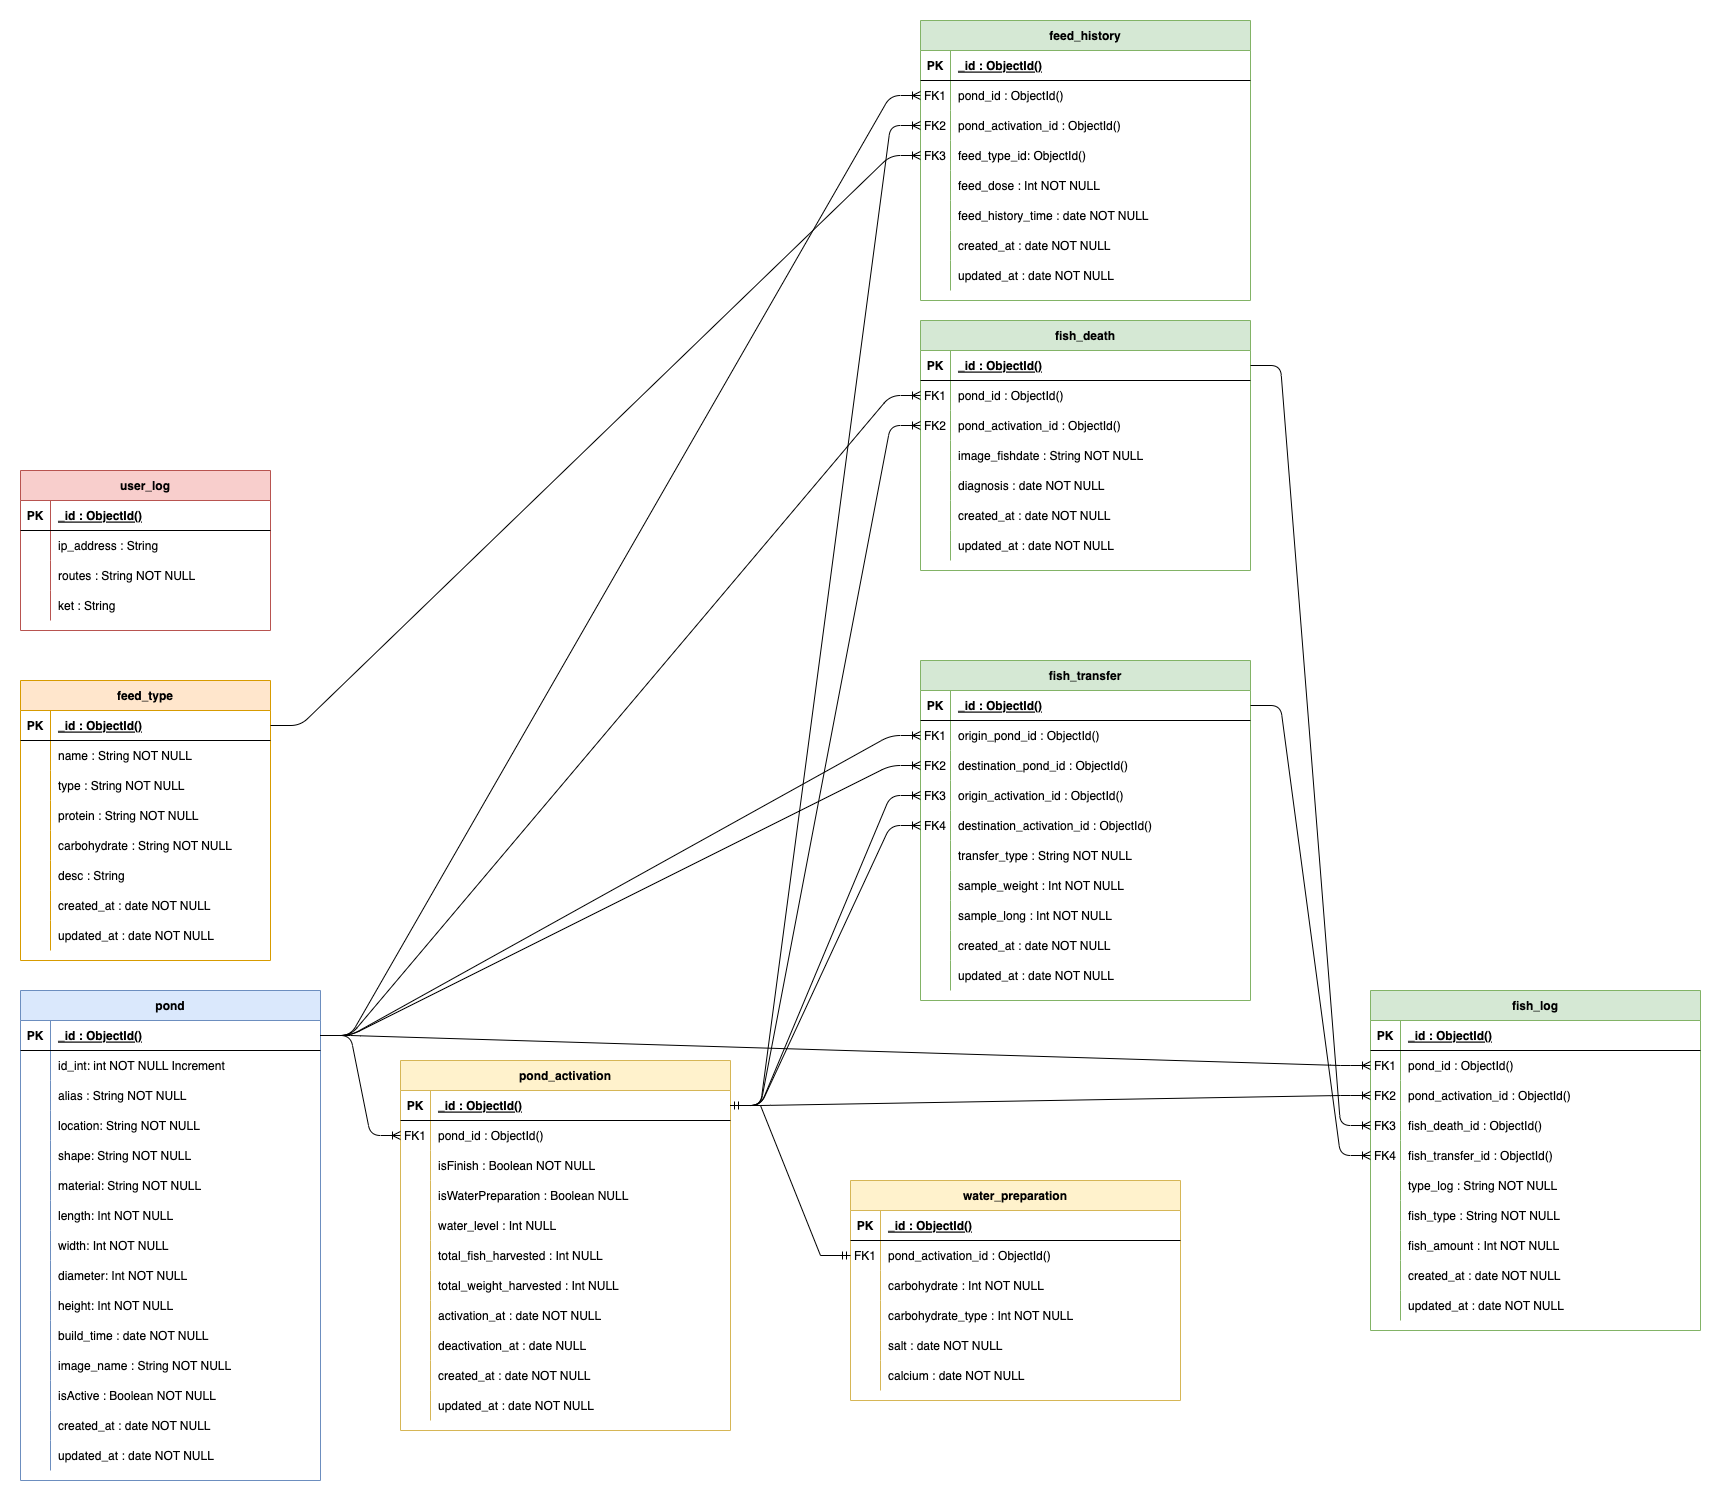
\includegraphics[height=0.7\textwidth]{gambar/Sprint07/diagram database/database}
	\caption{ERD Database Sprint-7}
	\label{fig:database_sprint7}
\end{figure}

Dengan berubahnya desain database diperlukan juga penambahan model pada source code, berikut perubahan pada source code model.

\begin{lstlisting}
# fishapi/database/model.py

class FishTransfer(db.Document):
    origin_pond_id = db.ReferenceField(Pond, required=True)
    destination_pond_id = db.ReferenceField(Pond, required=True)
    origin_activation_id = db.ReferenceField(PondActivation, required=True)
    destination_activation_id = db.ReferenceField(
        PondActivation, required=True)
    transfer_type = db.StringField(required=True)
    sample_weight = db.IntField(required=True)
    sample_long = db.IntField(required=True)
    created_at = db.DateTimeField(default=datetime.datetime.now)
    updated_at = db.DateTimeField(default=datetime.datetime.now)
\end{lstlisting}



\item \textbf{Menambahkan routes API}

\begin{lstlisting}
# fishapi/resource/routes.py

 # fish transfer
    api.add_resource(FishTransfersApi, '/api/fishtransfer')
    api.add_resource(FishTransferApi, '/api/fishtransfer/<id>')
\end{lstlisting}




\item \textbf{Implementasi controller entry perpindahan ikan}

Implementasi controller API entry perpindahan ikan, berikut merupakan perubahan source code controller API entry perpindahan ikan.

\begin{lstlisting}
# fishapi/database/fishtransfer.py

class FishTransfersApi(Resource):
    def post(self):
        try:
            origin_pond_id = request.form.get("origin_pond_id", None)
            origin_pond = Pond.objects.get(id=origin_pond_id)
            if origin_pond.isActive == False:
                response = {"message": "status pond is not active"}
                response = json.dumps(response, default=str)
                return Response(response, mimetype="application/json", status=400)
            origin_activation = PondActivation.objects(
                pond_id=origin_pond_id, isFinish=False).order_by('-activated_at').first()
            destination_pond_id = request.form.get("destination_pond_id", None)
            destination_pond = Pond.objects.get(id=destination_pond_id)
            if destination_pond.isActive == False:
                response = {"message": "status pond is not active"}
                response = json.dumps(response, default=str)
                return Response(response, mimetype="application/json", status=400)
            destination_activation = PondActivation.objects(
                pond_id=destination_pond_id, isFinish=False).order_by('-activated_at').first()
            fish_grading_id = request.form.get("fish_grading_id", None)
            transfer_type = request.form.get("transfer_type", None)
            transfer_method = request.form.get("transfer_method", None)
            sample_weight = request.form.get("sample_weight", None)
            sample_long = request.form.get("sample_long", None)
            fishes = request.form.get("fish", "[]")
            fishes = json.loads(fishes)
            if len(fishes) < 1:
                response = {"message": "There is no fish"}
                response = json.dumps(response, default=str)
                return Response(response, mimetype="application/json", status=400)
            # if transfer method is "kering" deactived pond
            if transfer_method == "kering":
                # update activation
                pond_deactivation_data = {
                    "isFinish": True,
                    "total_fish_harvested": request.form.get("total_fish_harvested", None),
                    "total_weight_harvested": request.form.get("total_weight_harvested", None),
                    "deactivated_at": request.form.get("deactivated_at", datetime.datetime.now()),
                    "deactivated_description": "sortir kering"
                }
                origin_activation.update(**pond_deactivation_data)
                pond.update(**{"isActive": False})
            # update fish grading [optional]
            if fish_grading_id and transfer_method != "kering":
                # pengecekan fish_grading
                fish_grading = FishGrading.objects.get(id=fish_grading_id)
                # update fishgrading
                if transfer_type == "oversized_transfer":
                    fish_grading.update(**{"isOversizeTransferred": True})
                else:
                    fish_grading.update(**{"isUndersizeTransferred": True})
            # save data
            data = {
                "origin_pond_id": origin_pond_id,
                "destination_pond_id": destination_pond_id,
                "origin_activation_id": origin_activation.id,
                "destination_activation_id": destination_activation.id,
                "fish_grading_id": None if transfer_method == "kering" else fish_grading_id,
                "transfer_type": None if transfer_method == "kering" else transfer_type,
                "transfer_method": transfer_method,
                "transfer_type": transfer_type,
                "sample_weight": sample_weight,
                "sample_long": sample_long
            }
            fish_transfer = FishTransfer(**data).save()
            # transfer out
            for fish in fishes:
                # save fish log
                data = {
                    "pond_id": origin_pond_id,
                    "pond_activation_id": origin_activation.id,
                    "fish_transfer_id": fish_transfer.id,
                    "type_log": "transfer_out",
                    "fish_type": fish['type'],
                    "fish_amount": fish['amount'] * -1
                }
                fishlog = FishLog(**data).save()
            # transfer in
            for fish in fishes:
                # save fish log
                data = {
                    "pond_id": destination_pond_id,
                    "pond_activation_id": destination_activation.id,
                    "fish_transfer_id": fish_transfer.id,
                    "type_log": "transfer_in",
                    "fish_type": fish['type'],
                    "fish_amount": fish['amount']
                }
                fishlog = FishLog(**data).save()
            response = {"message": "success add fishdeath"}
            response = json.dumps(response, default=str)
            return Response(response, mimetype="application/json", status=200)
        except Exception as e:
            response = {"message": str(e)}
            response = json.dumps(response, default=str)
            return Response(response, mimetype="application/json", status=400)
\end{lstlisting}

Pada awalnya, kode tersebut melakukan beberapa hal berikut:

\begin{enumerate}[(1)]
\item Menerima data dari permintaan POST yang dikirim oleh klien.
\item Memeriksa status kolam asal (origin\_pond) menggunakan origin\_pond\_id. Jika kolam tidak aktif, maka akan dikembalikan respons dengan pesan "status kolam tidak aktif".
\item Mengambil aktivasi kolam asal yang belum selesai (isFinish=False) berdasarkan origin\_pond\_id dan diurutkan berdasarkan waktu aktivasi terakhir (activated\_at).
\item Memeriksa status kolam tujuan (destination\_pond) menggunakan destination\_pond\_id. Jika kolam tidak aktif, maka akan dikembalikan respons dengan pesan "status kolam tidak aktif".
\item Mengambil aktivasi kolam tujuan yang belum selesai (isFinish=False) berdasarkan destination\_pond\_id dan diurutkan berdasarkan waktu aktivasi terakhir (activated\_at).
\end{enumerate}

Selanjutnya, kode tersebut melakukan beberapa tugas lainnya:

\begin{enumerate}[(1)]
\item Mengambil data seperti fish\_grading\_id, transfer\_type, transfer\_method, sample\_weight, sample\_long, dan fishes dari permintaan POST.
\item Memeriksa apakah terdapat ikan dalam fishes. Jika tidak ada ikan, maka akan dikembalikan respons dengan pesan "Tidak ada ikan".
\item Jika metode transfer adalah "kering", maka akan dilakukan deaktivasi kolam asal. Data aktivasi kolam akan diperbarui dengan mengatur isFinish menjadi True dan mengisi informasi terkait seperti jumlah ikan yang dipanen, bobot total yang dipanen, waktu deaktivasi, dan deskripsi deaktivasi.
\item Jika terdapat fish\_grading\_id dan metode transfer bukan "kering", maka akan dilakukan pembaruan pada penilaian ikan. Jika transfer\_type adalah "oversized\_transfer", maka isOversizeTransferred akan diatur sebagai True. Jika tidak, isUndersizeTransferred akan diatur sebagai True.
\item Data yang diperoleh akan disimpan dalam variabel data untuk digunakan nanti.
\item Dilakukan penyimpanan data transfer ikan menggunakan model FishTransfer.
\item Dilakukan transfer ikan keluar (transfer out) dan transfer ikan masuk (transfer in) untuk setiap ikan dalam fishes. Untuk setiap ikan, data log ikan akan disimpan menggunakan model FishLog.
\item Setelah semua operasi selesai, respons dengan pesan "success add fishdeath" akan dikirim kembali kepada klien.
\end{enumerate}

Jika terjadi kesalahan selama proses tersebut, akan ditangkap oleh blok except dan respons dengan pesan kesalahan yang sesuai akan dikirim kembali kepada klien.

Berikut merupakan form untuk entry perpindahan ikan antar kolam.

\begin{longtable}{| l | p{5cm} | p{5cm} |}
\caption{Form entry kematian ikan.\label{table:form_entry_kematian_ikan}}\\

\hline
\multicolumn{1}{|c|}{\textbf{Form}} & \multicolumn{1}{|c|}{\textbf{Jenis Data}} & \multicolumn{1}{|c|}{\textbf{Deskripsi}}\\
\hline
\endfirsthead

\hline
\multicolumn{3}{|c|}{Lanjutan Tabel \ref{table:form_entry_kematian_ikan}}\\
\hline
\multicolumn{1}{|c|}{\textbf{Form}} & \multicolumn{1}{|c|}{\textbf{Jenis Data}} & \multicolumn{1}{|c|}{\textbf{Deskripsi}}\\
\hline
\endhead

                                          

origin\_pond\_id         & REQUIRED STRING                                                                                                                                             & id kolam asal ikan yang akan di transfer                                                                                                                                                      \\ \hline
destination\_pond\_id    & REQUIRED STRING                                                                                                                                             & id kolam tujuan ikan yang akan di transfer                                                                                                                                                    \\ \hline
fish                     & REQUIRED JSON FISH TYPE: {[}"nila hitam", "nila merah", "lele", "patin", "mas",{]} Ex: {[}\{"type": "lele","amount": 5\},\{"type": "patin","amount": 9\}{]} & tipe dan banyak ikan                                                                                                                                                                          \\ \hline
transfer\_method         & REQUIRED STRING TYPE: {[}"kering","basah"{]}                                                                                                                & metode transfer ikan, jika kering kolam akan dianggap panen sekaligus                                                                                                                         \\ \hline
sample\_weight           & REQUIRED INT                                                                                                                                                & sample berat ikan yang dipindahkan                                                                                                                                                            \\ \hline
sample\_long             & REQUIRED INT                                                                                                                                                & sample panjang ikan yang dipindahkan                                                                                                                                                          \\ \hline
transfer\_type           & REQUIRED STRING TYPE; {[}"oversized\_transfer", "undersized\_transfer"{]}                                                                                    & tipe transfer, "oversized\_transfer" adalah perpindahan yang dilakukan karena ikan terlalu besar dari pada ikan yang ada di kolam asal, sedangkan "undersized\_transfer" adalah kebalikannya" \\ \hline
total\_fish\_harvested   & REQUIRED IF "transfer\_method" IS "kering" INT                                                                                                              & total ikan yang dipanen bila "transfer\_method" adalah "kering"                                                                                                                               \\ \hline
total\_weight\_harvested & REQUIRED IF "transfer\_method" IS "kering" INT                                                                                                              & total berat ikan yang dipanen bila "transfer\_method" adalah "kering"                                                                                                                         \\ \hline

\end{longtable}


Berikut adalah penjelasan rinci dari setiap kolom dalam tabel tersebut:

\begin{enumerate}
\item "origin\_pond\_id": Variabel yang diperlukan, berupa string yang mengidentifikasi ID kolam asal ikan yang akan ditransfer.
\item "destination\_pond\_id": Variabel yang diperlukan, berupa string yang mengidentifikasi ID kolam tujuan ikan yang akan ditransfer.
\item "fish": Variabel yang diperlukan, berupa JSON yang mengandung tipe dan jumlah ikan yang akan ditransfer. Contoh format JSON: [{"type": "lele", "amount": 5}, {"type": "patin", "amount": 9}]. Menggambarkan jenis dan jumlah ikan yang akan ditransfer.
\item "transfer\_method": Variabel yang diperlukan, berupa string yang mengindikasikan metode transfer ikan. Jika nilainya "kering", itu berarti kolam akan dianggap sedang dipanen secara keseluruhan. Jika nilainya "basah", maka transfer akan dilakukan dengan metode lain.
\item "sample\_weight": Variabel yang diperlukan, berupa bilangan bulat (integer) yang mewakili berat sampel ikan yang akan ditransfer.
\item "sample\_long": Variabel yang diperlukan, berupa bilangan bulat (integer) yang mewakili panjang sampel ikan yang akan ditransfer.
\item "transfer\_type": Variabel yang diperlukan, berupa string yang menentukan tipe transfer. Nilainya bisa "oversized\_transfer" jika ikan yang ditransfer terlalu besar dibandingkan dengan ikan di kolam asal, atau "undersized\_transfer" jika ikan yang ditransfer terlalu kecil dibandingkan dengan ikan di kolam asal.
\item "total\_fish\_harvested": Variabel yang diperlukan jika "transfer\_method" adalah "kering", berupa bilangan bulat (integer) yang mewakili total jumlah ikan yang dipanen.
\item "total\_weight\_harvested": Variabel yang diperlukan jika "transfer\_method" adalah "kering", berupa bilangan bulat (integer) yang mewakili total berat ikan yang dipanen.
\end{enumerate}

Berikut merupakan hasil test request dari API entry perpindahan ikan antar kolam.

cURL:

\begin{lstlisting}
curl --location 'http://jft.web.id/fishapi/api/fishtransfer' \
--form 'origin_pond_id="62a62163e445ffb9c5f746f3"' \
--form 'destination_pond_id="625d7033a9a73e090c65cda2"' \
--form 'fish="[{\"type\": \"lele\",\"amount\": 30},{\"type\": \"patin\",\"amount\": 10}]"' \
--form 'sample_weight="20"' \
--form 'sample_long="50"'
\end{lstlisting}

response json:

\begin{lstlisting}
{
  "message": "success add fishtransfer"
}
\end{lstlisting}




\item \textbf{Implementasi API fetch list perpindahan ikan}

Implementasi controller API fetch list perpindahan ikan, berikut merupakan source code controller API fetch list perpindahan ikan.

\begin{lstlisting}
# fishapi/resource/fishtransfer.py

def get(self):
        try:
            pipeline = [
                {'$lookup': {
                    'from': 'pond',
                    'let': {"pondid": "$origin_pond_id"},
                    'pipeline': [
                        {'$match': {
                            '$expr': {'$eq': ['$_id', '$$pondid']}}},
                        {"$project": {
                            "created_at": 0,
                            "updated_at": 0,
                        }}
                    ],
                    'as': 'origin_pond'
                }},
                {'$lookup': {
                    'from': 'pond',
                    'let': {"pondid": "$destination_pond_id"},
                    'pipeline': [
                        {'$match': {
                            '$expr': {'$eq': ['$_id', '$$pondid']}}},
                        {"$project": {
                            "created_at": 0,
                            "updated_at": 0,
                        }}
                    ],
                    'as': 'destination_pond'
                }},
                {"$addFields": {
                    "origin_pond": {"$first": "$origin_pond"},
                    "destination_pond": {"$first": "$destination_pond"},
                }},
                {'$lookup': {
                    'from': 'fish_log',
                    'let': {"fish_transfer_id": "$_id"},
                    'pipeline': [
                        {'$match': {
                            '$expr': {'$and': [
                                {'$eq': ['$fish_transfer_id',
                                         '$$fish_transfer_id']},
                                {'$eq': ['$type_log',
                                         'transfer_out']},
                            ]}
                        }},
                        {"$project": {
                            "created_at": 0,
                            "updated_at": 0,
                        }}
                    ],
                    'as': 'fish'
                }},
                {"$project": {
                    "updated_at": 0,
                    "created_at": 0,
                }}

            ]
            fishtransfers = FishTransfer.objects.aggregate(pipeline)
            fishtransfers = list(fishtransfers)
            response = json.dumps(fishtransfers, default=str)
            return Response(response, mimetype="application/json", status=200)
        except Exception as e:
            response = {"message": str(e)}
            response = json.dumps(response, default=str)
            return Response(response, mimetype="application/json", status=400)
\end{lstlisting}


Kode diatas adalah sebuah fungsi yang mengambil data transfer ikan dari database. Fungsi ini menggunakan operasi agregasi MongoDB untuk melakukan penggabungan (lookup) antara koleksi "fish\_transfer" dengan koleksi "pond" dan "fish\_log" untuk mengambil data terkait.

Pertama, fungsi ini mendefinisikan sebuah pipeline yang berisi serangkaian operasi agregasi. Operasi pertama adalah \$lookup yang menghubungkan koleksi "fish\_transfer" dengan koleksi "pond" berdasarkan origin\_pond\_id. Hasil penggabungan ini disimpan dalam field origin\_pond. Operasi yang sama juga dilakukan untuk menggabungkan koleksi "fish\_transfer" dengan koleksi "pond" berdasarkan destination\_pond\_id, dan hasilnya disimpan dalam field destination\_pond.

Selanjutnya, dilakukan operasi \$addFields untuk mengambil nilai pertama dari field origin\_pond dan destination\_pond, dan menyimpannya dalam field yang sama. Setelah itu, dilakukan \$lookup kembali untuk menggabungkan koleksi "fish\_transfer" dengan koleksi "fish\_log" berdasarkan \_id dari transfer ikan. Hasil penggabungan ini disimpan dalam field fish.

Akhirnya, dilakukan operasi \$project untuk menghilangkan field updated\_at dan created\_at dari hasil akhir. Seluruh pipeline diterapkan pada koleksi "fish\_transfer" menggunakan fungsi aggregate, dan hasilnya dikonversi menjadi daftar Python. Data tersebut kemudian diubah menjadi format JSON menggunakan json.dumps, dan dikembalikan sebagai respons dengan tipe konten "application/json" dan kode status 200.

Jika terjadi kesalahan selama proses, pengecualian akan ditangkap dan sebuah respons JSON yang berisi pesan kesalahan akan dikirim dengan tipe konten "application/json" dan kode status 400.

Berikut merupakan hasil test request dari API fetch list perpindahan ikan antar kolam.

cURL:

\begin{lstlisting}
curl --location 'http://jft.web.id/fishapi/api/fishtransfer'
\end{lstlisting}

response json:

\begin{lstlisting}
[
  {
    "_id": "62d564220d9bde3218b4951b",
    "origin_pond_id": "62a62163e445ffb9c5f746f3",
    "destination_pond_id": "625d7033a9a73e090c65cda2",
    "origin_activation_id": "62d3f2180d7265ab60f9cb83",
    "destination_activation_id": "62d562e676d3a668927c511f",
    "sample_weight": 20,
    "sample_long": 50,
    "origin_pond": {
      "_id": "62a62163e445ffb9c5f746f3",
      "id_int": 4,
      "alias": "charlie",
      "location": "blok 2",
      "shape": "persegi",
      "material": "tanah",
      "length": 5,
      "width": 3,
      "diameter": 0,
      "height": 1,
      "build_at": "2022-06-13 00:24:51.473000",
      "image_name": "kolam_1656312365.jpeg",
      "isActive": true
    },
    "destination_pond": {
      "_id": "625d7033a9a73e090c65cda2",
      "id_int": 3,
      "alias": "beta",
      "location": "blok 10",
      "shape": "persegi",
      "material": "terpal",
      "length": 8,
      "width": 4,
      "diameter": 0,
      "height": 1,
      "build_at": "2022-04-18 21:05:39.608000",
      "image_name": "default.jpg",
      "isActive": true
    },
    "fish": [
      {
        "_id": "62d564220d9bde3218b4951c",
        "pond_id": "62a62163e445ffb9c5f746f3",
        "pond_activation_id": "62d3f2180d7265ab60f9cb83",
        "fish_transfer_id": "62d564220d9bde3218b4951b",
        "type_log": "transfer_out",
        "fish_type": "lele",
        "fish_amount": -20
      },
      {
        "_id": "62d564220d9bde3218b4951d",
        "pond_id": "62a62163e445ffb9c5f746f3",
        "pond_activation_id": "62d3f2180d7265ab60f9cb83",
        "fish_transfer_id": "62d564220d9bde3218b4951b",
        "type_log": "transfer_out",
        "fish_type": "patin",
        "fish_amount": -20
      }
    ]
  },
  {
    "_id": "62d57d8b08d03adbb8cff042",
    "origin_pond_id": "62a62163e445ffb9c5f746f3",
    "destination_pond_id": "625d7033a9a73e090c65cda2",
    "origin_activation_id": "62d3f2180d7265ab60f9cb83",
    "destination_activation_id": "62d562e676d3a668927c511f",
    "sample_weight": 20,
    "sample_long": 50,
    "origin_pond": {
      "_id": "62a62163e445ffb9c5f746f3",
      "id_int": 4,
      "alias": "charlie",
      "location": "blok 2",
      "shape": "persegi",
      "material": "tanah",
      "length": 5,
      "width": 3,
      "diameter": 0,
      "height": 1,
      "build_at": "2022-06-13 00:24:51.473000",
      "image_name": "kolam_1656312365.jpeg",
      "isActive": true
    },
    "destination_pond": {
      "_id": "625d7033a9a73e090c65cda2",
      "id_int": 3,
      "alias": "beta",
      "location": "blok 10",
      "shape": "persegi",
      "material": "terpal",
      "length": 8,
      "width": 4,
      "diameter": 0,
      "height": 1,
      "build_at": "2022-04-18 21:05:39.608000",
      "image_name": "default.jpg",
      "isActive": true
    },
    "fish": [
      {
        "_id": "62d57d8b08d03adbb8cff043",
        "pond_id": "62a62163e445ffb9c5f746f3",
        "pond_activation_id": "62d3f2180d7265ab60f9cb83",
        "fish_transfer_id": "62d57d8b08d03adbb8cff042",
        "type_log": "transfer_out",
        "fish_type": "lele",
        "fish_amount": -30
      },
      {
        "_id": "62d57d8b08d03adbb8cff044",
        "pond_id": "62a62163e445ffb9c5f746f3",
        "pond_activation_id": "62d3f2180d7265ab60f9cb83",
        "fish_transfer_id": "62d57d8b08d03adbb8cff042",
        "type_log": "transfer_out",
        "fish_type": "patin",
        "fish_amount": -10
      }
    ]
  }
]
\end{lstlisting}



\item \textbf{Implementasi API edit perpindahan ikan}

Implementasi controller API edit perpindahan ikan, berikut merupakan perubahan source code controller API edit perpindahan ikan.

\begin{lstlisting}
# fishapi/database/fishtransfer.py

def put(self, id):
        try:
            body = request.form.to_dict(flat=True)
            FishDeath.objects.get(id=id).update(**body)
            response = {"message": "success change data fish death", "id": id}
            response = json.dumps(response, default=str)
            return Response(response, mimetype="application/json", status=200)
        except Exception as e:
            response = {"message": str(e)}
            response = json.dumps(response, default=str)
            return Response(response, mimetype="application/json", status=400)
\end{lstlisting}

Kode di atas adalah sebuah fungsi yang digunakan untuk mengubah data kematian ikan dalam database. Fungsi ini menerima parameter id yang merupakan ID unik dari data kematian ikan yang ingin diubah.

Pada awalnya, fungsi ini mengambil data dari permintaan (request) dalam bentuk formulir dan mengonversinya menjadi kamus (dictionary) menggunakan metode to\_dict(flat=True). Kamus ini kemudian disimpan dalam variabel body.

Selanjutnya, fungsi ini menggunakan metode get() dari model FishDeath untuk mendapatkan objek kematian ikan berdasarkan ID yang diberikan. Setelah itu, metode update() dipanggil pada objek tersebut dengan meneruskan body sebagai argumen. Ini akan mengubah nilai-nilai properti objek sesuai dengan nilai-nilai dalam kamus body.

Setelah berhasil mengubah data kematian ikan, fungsi ini mengembalikan respons sukses dalam format JSON. Pesan respons berisi informasi bahwa data kematian ikan telah berhasil diubah, beserta ID dari data yang telah diubah. Pesan respons kemudian diubah menjadi bentuk JSON menggunakan json.dumps, dan dikembalikan sebagai respons dengan tipe konten "application/json" dan kode status 200.

Namun, jika terjadi kesalahan selama proses, pengecualian akan ditangkap dan sebuah respons JSON yang berisi pesan kesalahan akan dikirim. Pesan kesalahan akan menampilkan detail dari pengecualian yang terjadi. Respons JSON tersebut juga dikembalikan dengan tipe konten "application/json" dan kode status 400.

Berikut merupakan hasil test request dari API edit perpindahan ikan antar kolam.

cURL:

\begin{lstlisting}
curl --location -g --request PUT 'http://jft.web.id/fishapi/api/fishtransfer/{fishtransfer_id}' \
--form 'sample_weight="20"' \
\end{lstlisting}

response json:

\begin{lstlisting}
{
  "message": "success change data fish transfer",
  "id": "62b9adfa793e0f39dbaa1739"
}
\end{lstlisting}



\item \textbf{Implementasi API delete perpindahan ikan}

Implementasi controller API delete perpindahan ikan, berikut merupakan perubahan source code controller API delete perpindahan ikan.

\begin{lstlisting}
# fishapi/database/fishtransfer.py

def delete(self, id):
        try:
            fishtransfer = FishTransfer.objects.get(id=id)
            # delete fish
            fishes = FishLog.objects.aggregate([
                {'$match': {
                    '$expr': {'$eq': ['$fish_transfer_id', {'$toObjectId': id}]}}},
            ])
            for fish in fishes:
                fishlog = FishLog.objects.get(id=fish['_id'])
                fishlog.delete()
            # delete data
            fishtransfer.delete()
            response = {"message": "success delete fishtransfer"}
            response = json.dumps(response, default=str)
            return Response(response, mimetype="application/json", status=200)
        except Exception as e:
            response = {"message": str(e)}
            response = json.dumps(response, default=str)
            return Response(response, mimetype="application/json", status=400)
\end{lstlisting}

Kode di atas merupakan sebuah fungsi yang digunakan untuk menghapus data transfer ikan dari database. Fungsi ini menerima parameter id yang merupakan ID unik dari data transfer ikan yang akan dihapus.

Pada awalnya, fungsi ini menggunakan metode get() dari model FishTransfer untuk mendapatkan objek transfer ikan berdasarkan ID yang diberikan. Objek tersebut disimpan dalam variabel fishtransfer.

Selanjutnya, fungsi ini menggunakan agregasi MongoDB untuk mencari dan mendapatkan daftar ikan yang terkait dengan transfer ikan yang akan dihapus. Pencarian dilakukan berdasarkan kesesuaian nilai fish\_transfer\_id dengan ID transfer ikan yang diberikan. Hasil pencarian tersebut disimpan dalam variabel fishes.

Setelah mendapatkan daftar ikan terkait, fungsi ini melakukan iterasi melalui daftar tersebut. Pada setiap iterasi, fungsi menghapus objek FishLog yang sesuai dengan ID ikan yang ditemukan.

Setelah menghapus semua data ikan terkait, fungsi ini menghapus objek transfer ikan itu sendiri dengan menggunakan metode delete() pada objek fishtransfer.

Setelah berhasil menghapus data transfer ikan, fungsi ini mengembalikan respons sukses dalam format JSON. Pesan respons menyatakan bahwa data transfer ikan telah berhasil dihapus. Pesan respons kemudian diubah menjadi bentuk JSON menggunakan json.dumps, dan dikembalikan sebagai respons dengan tipe konten "application/json" dan kode status 200.

Namun, jika terjadi kesalahan selama proses, pengecualian akan ditangkap dan sebuah respons JSON yang berisi pesan kesalahan akan dikirim. Pesan kesalahan akan menampilkan detail dari pengecualian yang terjadi. Respons JSON tersebut juga dikembalikan dengan tipe konten "application/json" dan kode status 400.

Berikut merupakan hasil test request dari API delete perpindahan ikan antar kolam.

cURL:

\begin{lstlisting}
curl --location --request DELETE 'http://jft.web.id/fishapi/api/fishtransfer/62d564220d9bde3218b4951b'
\end{lstlisting}

response json:

\begin{lstlisting}
{
  "message": "success delete fishtransfer"
}
\end{lstlisting}


\item \textbf{Implementasi API fetch detail perpindahan ikan}

Implementasi controller API fetch detail perpindahan ikan, berikut merupakan source code controller API fetch detail perpindahan ikan.

\begin{lstlisting}
# fishapi/resource/fishtransfer.py

def get(self, id):
        try:
            pipeline = [
                {'$match': {'$expr': {'$eq': ['$_id', {'$toObjectId': id}]}}},
                {'$lookup': {
                    'from': 'pond',
                    'let': {"pondid": "$origin_pond_id"},
                    'pipeline': [
                        {'$match': {
                            '$expr': {'$eq': ['$_id', '$$pondid']}}},
                        {"$project": {
                            "created_at": 0,
                            "updated_at": 0,
                        }}
                    ],
                    'as': 'origin_pond'
                }},
                {'$lookup': {
                    'from': 'pond',
                    'let': {"pondid": "$destination_pond_id"},
                    'pipeline': [
                        {'$match': {
                            '$expr': {'$eq': ['$_id', '$$pondid']}}},
                        {"$project": {
                            "created_at": 0,
                            "updated_at": 0,
                        }}
                    ],
                    'as': 'destination_pond'
                }},
                {"$addFields": {
                    "origin_pond": {"$first": "$origin_pond"},
                    "destination_pond": {"$first": "$destination_pond"},
                }},
                {'$lookup': {
                    'from': 'fish_log',
                    'let': {"fish_transfer_id": "$_id"},
                    'pipeline': [
                        {'$match': {
                            '$expr': {'$and': [
                                {'$eq': ['$fish_transfer_id',
                                         '$$fish_transfer_id']},
                                {'$eq': ['$type_log',
                                         'transfer_out']},
                            ]}
                        }},
                        {"$project": {
                            "created_at": 0,
                            "updated_at": 0,
                        }}
                    ],
                    'as': 'fish'
                }},
                {"$project": {
                    "updated_at": 0,
                    "created_at": 0,
                }}

            ]
            fishtransfers = FishTransfer.objects.aggregate(pipeline)
            fishtransfers = list(fishtransfers)
            fishtransfer = fishtransfers[0]
            response = json.dumps(fishtransfer, default=str)
            return Response(response, mimetype="application/json", status=200)
        except Exception as e:
            response = {"message": str(e)}
            response = json.dumps(response, default=str)
            return Response(response, mimetype="application/json", status=400)
\end{lstlisting}


Kode di atas merupakan sebuah fungsi yang digunakan untuk mendapatkan data transfer ikan berdasarkan ID dari database. Fungsi ini menerima parameter id yang merupakan ID unik dari transfer ikan yang ingin diperoleh.

Pada awalnya, fungsi ini menggunakan agregasi MongoDB dengan pipeline untuk mencocokkan transfer ikan berdasarkan kesesuaian ID dengan ID yang diberikan. Pipeline ini terdiri dari beberapa tahap:

\begin{enumerate}
\item Tahap pertama, \$match, digunakan untuk mencocokkan dokumen berdasarkan nilai \_id yang sama dengan ID yang diberikan.

\item Selanjutnya, terdapat dua tahap \$lookup yang digunakan untuk melakukan operasi join dengan koleksi "pond". Kedua tahap ini berguna untuk mencari informasi kolam asal dan kolam tujuan dari transfer ikan. Kedua tahap ini menggunakan variabel \$origin\_pond\_id dan \$destination\_pond\_id untuk mencocokkan nilai \_id dengan nilai dari kolom tersebut di koleksi "pond". Tahap ini juga menggunakan tahap \$project untuk menghilangkan field "created\_at" dan "updated\_at" dari hasil join.

\item Setelah itu, menggunakan tahap \$addFields, ditambahkan dua field baru, yaitu "origin\_pond" dan "destination\_pond", yang nilainya diambil dari hasil join sebelumnya. Field-field ini hanya mengambil nilai pertama dari hasil join menggunakan operator \$first.

\item Kemudian, terdapat tahap \$lookup lainnya untuk melakukan operasi join dengan koleksi "fish\_log". Tahap ini mencari log ikan yang terkait dengan transfer ikan berdasarkan nilai \_id transfer ikan tersebut. Pencocokan dilakukan berdasarkan nilai \$fish\_transfer\_id dengan nilai dari field \_id di koleksi "fish\_log". Seperti sebelumnya, tahap ini juga menggunakan tahap \$project untuk menghilangkan field "created\_at" dan "updated\_at" dari hasil join.

\item Terakhir, menggunakan tahap \$project, dihilangkan juga field "updated\_at" dan "created\_at" dari hasil akhir.
\end{enumerate}

Setelah pipeline selesai, fungsi ini menggunakan metode aggregate() dari model FishTransfer dengan menggunakan pipeline yang telah dibuat untuk mendapatkan hasilnya. Hasilnya kemudian dikonversi menjadi list dan disimpan dalam variabel fishtransfers. Karena hanya ingin mendapatkan satu transfer ikan berdasarkan ID, maka transfer ikan pertama dari list tersebut diambil dan disimpan dalam variabel fishtransfer.

Selanjutnya, hasil transfer ikan tersebut diubah menjadi bentuk JSON menggunakan json.dumps(). JSON tersebut kemudian dikembalikan sebagai respons dengan tipe konten "application/json" dan kode status 200.

Namun, jika terjadi kesalahan selama proses, pengecualian akan ditangkap dan sebuah respons JSON yang berisi pesan kesalahan akan dikirim. Pesan kesalahan akan menampilkan detail dari pengecualian yang terjadi. Respons JSON tersebut juga dikembalikan dengan tipe konten "application/json" dan kode status 400.

Berikut merupakan hasil test request dari API fetch list perpindahan ikan antar kolam.

cURL:

\begin{lstlisting}
curl --location 'http://jft.web.id/fishapi/api/fishtransfer/62d564220d9bde3218b4951b'
\end{lstlisting}

response json:

\begin{lstlisting}
{
  "_id": "62d564220d9bde3218b4951b",
  "origin_pond_id": "62a62163e445ffb9c5f746f3",
  "destination_pond_id": "625d7033a9a73e090c65cda2",
  "origin_activation_id": "62d3f2180d7265ab60f9cb83",
  "destination_activation_id": "62d562e676d3a668927c511f",
  "sample_weight": 20,
  "sample_long": 50,
  "origin_pond": {
    "_id": "62a62163e445ffb9c5f746f3",
    "id_int": 4,
    "alias": "charlie",
    "location": "blok 2",
    "shape": "persegi",
    "material": "tanah",
    "length": 5,
    "width": 3,
    "diameter": 0,
    "height": 1,
    "build_at": "2022-06-13 00:24:51.473000",
    "image_name": "kolam_1656312365.jpeg",
    "isActive": true
  },
  "destination_pond": {
    "_id": "625d7033a9a73e090c65cda2",
    "id_int": 3,
    "alias": "beta",
    "location": "blok 10",
    "shape": "persegi",
    "material": "terpal",
    "length": 8,
    "width": 4,
    "diameter": 0,
    "height": 1,
    "build_at": "2022-04-18 21:05:39.608000",
    "image_name": "default.jpg",
    "isActive": true
  },
  "fish": [
    {
      "_id": "62d564220d9bde3218b4951c",
      "pond_id": "62a62163e445ffb9c5f746f3",
      "pond_activation_id": "62d3f2180d7265ab60f9cb83",
      "fish_transfer_id": "62d564220d9bde3218b4951b",
      "type_log": "transfer_out",
      "fish_type": "lele",
      "fish_amount": -20
    },
    {
      "_id": "62d564220d9bde3218b4951d",
      "pond_id": "62a62163e445ffb9c5f746f3",
      "pond_activation_id": "62d3f2180d7265ab60f9cb83",
      "fish_transfer_id": "62d564220d9bde3218b4951b",
      "type_log": "transfer_out",
      "fish_type": "patin",
      "fish_amount": -20
    }
  ]
}
\end{lstlisting}



\end{enumerate}
%!TEX root = ./template-skripsi.tex

\subsection{Sprint 8 Report}
Berikut merupakan report dari sprint ke-8 yang dilakukan pada tanggal 13 juli - 19 juli 2022.

\begin{table}[H]
	\caption{\textit{Sprint-8 backlog}}
	\label{sprint8_backlog}
	\begin{tabular}{@{} |p{0.5cm}|p{5cm}|p{5cm}|p{2cm}| @{}}
		\hline
		\textbf{No} & \textbf{\textit{Story}} & \textbf{\textit{Task}} & \textbf{\textit{Status}} \\
		\hline
		1 & \multirow{3}{5cm}{Create, Read, Updte, dan Delete untuk Pencatatan grading berat ikan} & Membarui desain database  & Completed\\
		\cline{1-1}\cline{3-4}
		2 & & Menambahkan routes API & Completed\\
		\cline{1-1}\cline{3-4}
		3 & & Implementasi controller entry grading berat ikan & Completed\\
		\cline{1-1}\cline{3-4}
		4 & & Implementasi controller fetch list grading berat ikan & Completed\\
		\cline{1-1}\cline{3-4}
		5 & & Implementasi controller edit grading berat ikan & Completed\\
		\cline{1-1}\cline{3-4}
		6 & & Implementasi controller delete grading berat ikan & Completed\\
		\cline{1-1}\cline{3-4}
		7 & & Implementasi controller fetch grading berat ikan dengan id& Completed\\
		\cline{1-1}\cline{3-4}
		8 & & Membuat view rekap grading berat ikan & Completed\\
		\cline{1-1}\cline{3-4}
		\hline
	\end{tabular}
\end{table}

\begin{enumerate}[1.]

\item \textbf{Membarui desain database}

\begin{figure}[H]
	\centering
	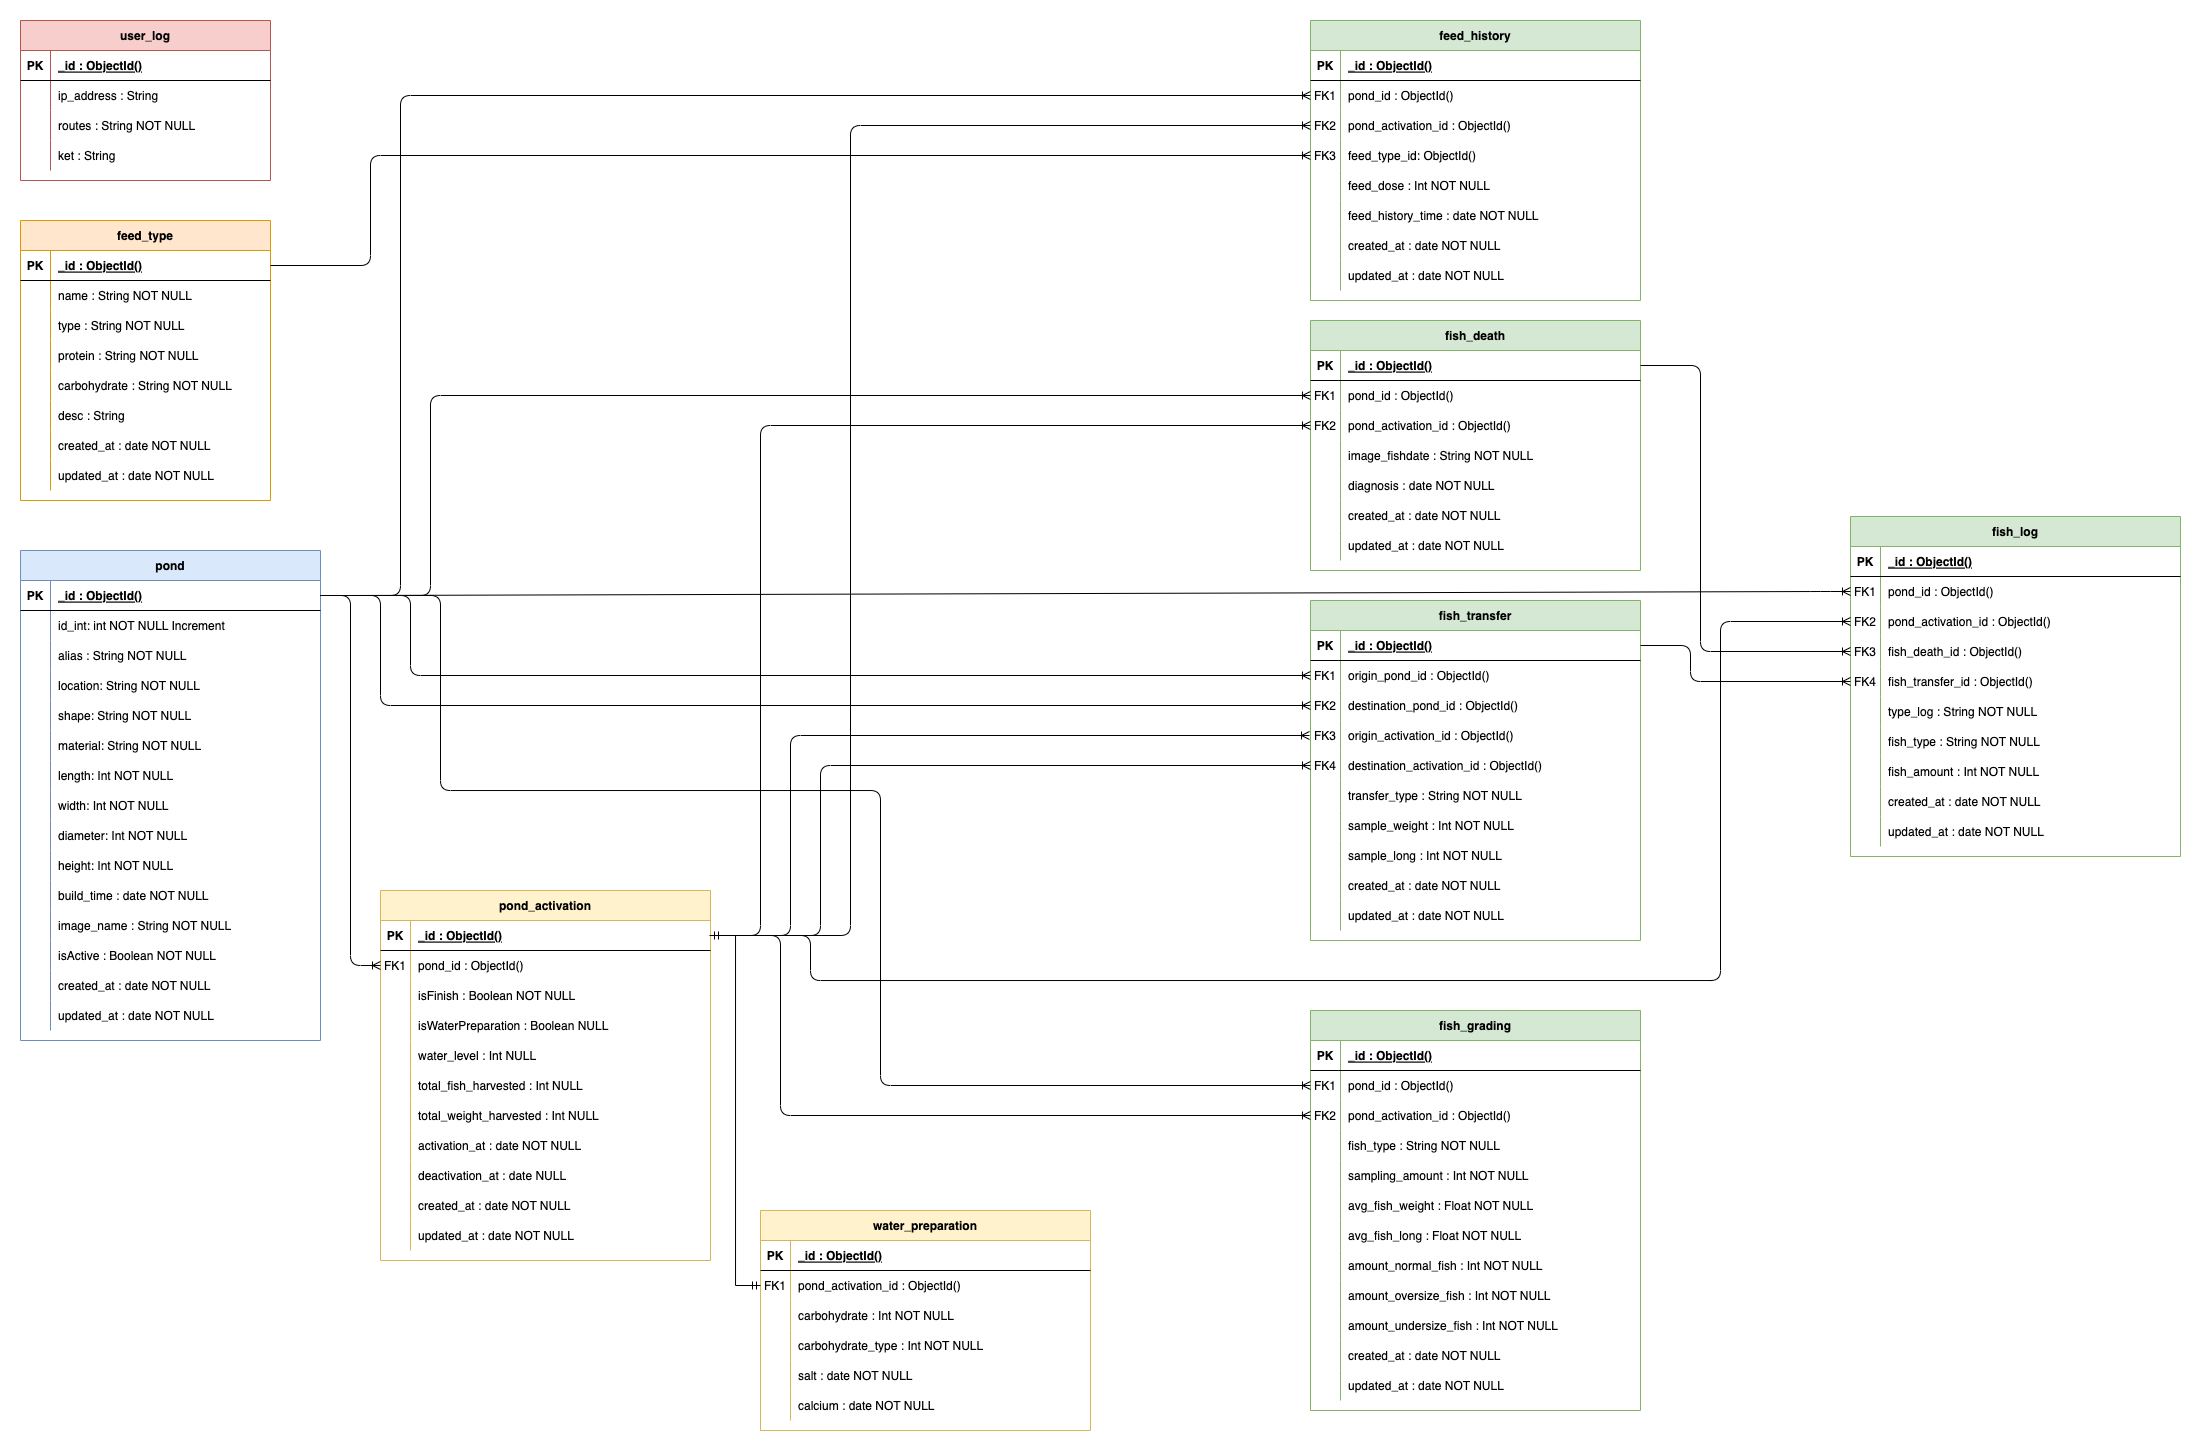
\includegraphics[height=0.7\textwidth]{gambar/Sprint08/diagram database/database}
	\caption{ERD Database Sprint-8}
	\label{fig:database_sprint8}
\end{figure}

Dengan berubahnya desain database diperlukan juga penambahan model pada source code, berikut perubahan pada source code model.

\begin{lstlisting}
# fishapi/database/model.py

class FishGrading(db.Document):
    pond_id = db.ReferenceField(Pond, required=True)
    pond_activation_id = db.ReferenceField(PondActivation, required=True)
    isOversizeTransferred = db.BooleanField(required=True, default=False)
    isUndersizeTransferred = db.BooleanField(required=True, default=False)
    fish_type = db.StringField(required=True)
    sampling_amount = db.IntField(required=True)
    avg_fish_weight = db.FloatField(required=True)
    avg_fish_long = db.FloatField(required=True)
    amount_normal_fish = db.IntField(required=True)
    amount_oversize_fish = db.IntField(required=True)
    amount_undersize_fish = db.IntField(required=True)
    grading_at = db.DateTimeField(default=datetime.datetime.now)
    created_at = db.DateTimeField(default=datetime.datetime.now)
    updated_at = db.DateTimeField(default=datetime.datetime.now)
\end{lstlisting}



\item \textbf{Menambahkan routes API}

\begin{lstlisting}
# fishapi/resource/routes.py

# fish grading
    api.add_resource(FishGradingsApi, '/api/fishgradings')
    api.add_resource(FishGradingApi, '/api/fishgradings/<id>')
    api.add_resource(FishGradingApiByActivation,
                     '/api/fishgradings/activation/<activation_id>')
    # graph
    api.add_resource(FishGradingGraphApi,
                     '/api/fishgradings/graph', endpoint='api.graph')
\end{lstlisting}




\item \textbf{Implementasi controller entry grading berat ikan}

Implementasi controller API entry grading berat ikan, berikut merupakan perubahan source code controller API entry grading berat ikan.

\begin{lstlisting}
# fishapi/resource/fishgrading.py

class FishGradingsApi(Resource):
    def post(self):
        try:
            pond_id = request.form.get("pond_id", None)
            pond = Pond.objects.get(id=pond_id)
            if pond['isActive'] == False:
                response = {"message": "pond is not active"}
                response = json.dumps(response, default=str)
                return Response(response, mimetype="application/json", status=400)
            pond_activation = PondActivation.objects(
                pond_id=pond_id, isFinish=False).order_by('-activated_at').first()
            body = {
                "pond_id": pond.id,
                "pond_activation_id": pond_activation.id,
                "fish_type": request.form.get("fish_type", None),
                "sampling_amount": request.form.get("sampling_amount", None),
                "avg_fish_weight": request.form.get("avg_fish_weight", None),
                "avg_fish_long": request.form.get("avg_fish_long", None),
                "amount_normal_fish": request.form.get("amount_normal_fish", None),
                "amount_oversize_fish": request.form.get("amount_oversize_fish", None),
                "amount_undersize_fish": request.form.get("amount_undersize_fish", None),
                "created_at": created_at,
                "grading_at": created_at,
            }
            fishgrading = FishGrading(**body).save()
            id = fishgrading.id
            return {'id': str(id)}, 200
        except Exception as e:
            response = {"message": str(e)}
            response = json.dumps(response, default=str)
            return Response(response, mimetype="application/json", status=400)
\end{lstlisting}

Kode di atas adalah sebuah API untuk mengelola data grading ikan. API ini menggunakan framework Flask-RESTful dan memiliki dua metode, yaitu get dan post.

Metode get digunakan untuk mendapatkan daftar grading ikan. Pada metode ini, digunakan agregasi MongoDB dengan pipeline untuk melakukan beberapa tahap pengolahan data. Pertama, terdapat dua tahap \$lookup yang digunakan untuk melakukan operasi join dengan koleksi "pond" dan "pond\_activation". Tahap-tahap ini mencocokkan nilai \_id dari transfer ikan dengan nilai dari field "pond\_id" dan "pond\_activation\_id" di koleksi yang di-lookup. Setelah itu, dengan menggunakan tahap \$addFields, ditambahkan dua field baru yaitu "pond" dan "pond\_activation" yang nilainya diambil dari hasil join sebelumnya menggunakan operator \$first. Tahap \$project digunakan untuk menghilangkan field "updated\_at" dan "created\_at" dari hasil akhir.

Setelah pipeline selesai, fungsi ini menggunakan metode aggregate() dari model FishGrading dengan menggunakan pipeline yang telah dibuat untuk mendapatkan hasilnya. Hasilnya kemudian dikonversi menjadi list dan disimpan dalam variabel list\_fishgradings.

Selanjutnya, hasil grading ikan tersebut diubah menjadi bentuk JSON menggunakan json.dumps(). JSON tersebut kemudian dikembalikan sebagai respons dengan tipe konten "application/json" dan kode status 200.

Jika terjadi kesalahan selama proses, pengecualian akan ditangkap dan sebuah respons JSON yang berisi pesan kesalahan akan dikirim. Pesan kesalahan akan menampilkan detail dari pengecualian yang terjadi. Respons JSON tersebut juga dikembalikan dengan tipe konten "application/json" dan kode status 400.

Metode post digunakan untuk membuat data grading ikan baru. Pada metode ini, terlebih dahulu dilakukan pengambilan nilai pond\_id dari form data yang dikirim. Kemudian, dilakukan pencarian kolam ("pond") berdasarkan pond\_id tersebut. Jika kolam tidak aktif (nilai "isActive" adalah False), maka dikembalikan respons JSON dengan pesan "pond is not active" dan kode status 400.

Selanjutnya, dilakukan pencarian aktivasi kolam ("pond\_activation") terbaru yang belum selesai (nilai "isFinish" adalah False) berdasarkan pond\_id. Nilai ini digunakan untuk mengisi field "pond\_activation\_id" pada data grading ikan yang akan dibuat.

Data grading ikan yang akan dibuat terdiri dari beberapa field yang diambil dari form data yang dikirim. Field "created\_at" dan "grading\_at" diisi dengan waktu saat ini. Data grading ikan tersebut kemudian disimpan ke dalam database menggunakan metode save().

Setelah data berhasil disimpan, ID dari data grading ikan yang baru dibuat diambil dan dikembalikan sebagai respons JSON dengan kode status 200.

Jika terjadi kesalahan selama proses, pengecualian akan ditangkap dan sebuah respons JSON yang berisi pesan kesalahan akan dikirim. Pesan kesalahan akan menampilkan detail dari pengecualian yang terjadi. Respons JSON tersebut juga dikembalikan dengan tipe konten "application/json" dan kode status 400.


Berikut merupakan form untuk entry grading berat ikan antar kolam.

\begin{longtable}{| l | p{5cm} | p{5cm} |}
\caption{Form entry kematian ikan.\label{table:form_entry_grading_berat_ikan}}\\

\hline
\multicolumn{1}{|c|}{\textbf{Form}} & \multicolumn{1}{|c|}{\textbf{Jenis Data}} & \multicolumn{1}{|c|}{\textbf{Deskripsi}}\\
\hline
\endfirsthead

\hline
\multicolumn{3}{|c|}{Lanjutan Tabel \ref{table:form_entry_grading_berat_ikan}}\\
\hline
\multicolumn{1}{|c|}{\textbf{Form}} & \multicolumn{1}{|c|}{\textbf{Jenis Data}} & \multicolumn{1}{|c|}{\textbf{Deskripsi}}\\
\hline
\endhead

                                          

pond\_id                & REQUIRED STRING                                                                & id kolam saat melakukan grading berat                                    \\ \hline
constanta\_oversize     & REQUIRED DOUBLE                                                                & konstanta yang menentukan berapa berat ikan yang dikategorikan oversize  \\ \hline
constanta\_undersize    & REQUIRED DOUBLE                                                                & konstanta yang menentukan berapa berat ikan yang dikategorikan undersize \\ \hline
fish\_type              & REQUIRED STRING TYPE; {[}"lele", "patin", "nila merah", "nila hitam", "mas"{]} & tipe ikan yang di grading beratnya                                       \\ \hline
sampling\_amount        & REQUIRED INT                                                                   & total jumlah ikan yang di lakukan sampling berat                         \\ \hline
avg\_fish\_weight       & REQUIRED DOUBLE                                                                & rata-rata berat ikan yang di sampling                                    \\ \hline
avg\_fish\_long         & REQUIRED DOUBLE                                                                & rata-rata panjang ikan yang di sampling                                  \\ \hline
amount\_normal\_fish    & REQUIRED INT                                                                   & jumlah ikan yang dikategorikan normal                                    \\ \hline
amount\_oversize\_fish  & REQUIRED INT                                                                   & jumlah ikan yang oversize                                                \\ \hline
amount\_undersize\_fish & REQUIRED INT                                                                   & jumlah ikan yang undersize                                               \\ \hline
\end{longtable}


Tabel di atas merupakan deskripsi dari kolom-kolom yang digunakan dalam suatu entitas data grading ikan. Tabel ini menjelaskan setiap kolom beserta tipe datanya dan penjelasan singkat tentang fungsinya.

Kolom pertama adalah "pond\_id" yang merupakan kolom wajib dengan tipe data STRING. Kolom ini digunakan untuk menyimpan ID kolam tempat dilakukannya grading berat pada ikan.

Kolom kedua dan ketiga adalah "constanta\_oversize" dan "constanta\_undersize" yang merupakan kolom wajib dengan tipe data DOUBLE. Kedua kolom ini digunakan untuk menyimpan konstanta yang menentukan batas berat ikan yang dikategorikan sebagai oversize atau undersize.

Kolom berikutnya adalah "fish\_type" yang merupakan kolom wajib dengan tipe data STRING. Kolom ini digunakan untuk menyimpan tipe ikan yang sedang dilakukan grading berat.

Selanjutnya, terdapat kolom "sampling\_amount" yang merupakan kolom wajib dengan tipe data INT. Kolom ini digunakan untuk menyimpan total jumlah ikan yang dilakukan sampling berat.

Kolom "avg\_fish\_weight" dan "avg\_fish\_long" adalah kolom wajib dengan tipe data DOUBLE. Kolom-kolom ini digunakan untuk menyimpan rata-rata berat dan panjang ikan yang diambil sebagai sampel.

Kolom "amount\_normal\_fish", "amount\_oversize\_fish", dan "amount\_undersize\_fish" adalah kolom wajib dengan tipe data INT. Kolom-kolom ini digunakan untuk menyimpan jumlah ikan yang dikategorikan sebagai normal, oversize, dan undersize, sesuai dengan hasil grading berat yang dilakukan.


Berikut merupakan hasil test request dari API entry perpindahan ikan antar kolam.

cURL:

\begin{lstlisting}
curl --location 'http://jft.web.id/fishapi/api/fishgradings' \
--form 'pond_id="{pond_id}"' \
--form 'fish_type="lele"' \
--form 'sampling_amount="20"' \
--form 'avg_fish_weight="50"' \
--form 'avg_fish_long="10"' \
--form 'amount_normal_fish="18"' \
--form 'amount_oversize_fish="1"' \
--form 'amount_undersize_fish="1"'
\end{lstlisting}

response json:

\begin{lstlisting}
{
  "message": "success add fish grading",
  "id": "62e105707ac8f837667faa70"
}
\end{lstlisting}




\item \textbf{Implementasi API fetch list grading berat ikan}

Implementasi controller API fetch list grading berat ikan, berikut merupakan source code controller API fetch list grading berat ikan.

\begin{lstlisting}
# fishapi/resource/fishgrading.py

def get(self):
        try:
            pipeline = [
                {'$lookup': {
                    'from': 'pond',
                    'let': {"pondid": "$pond_id"},
                    'pipeline': [
                        {'$match': {'$expr': {'$eq': ['$_id', '$$pondid']}}},
                        {"$project": {
                            "_id": 1,
                            "alias": 1,
                            "location": 1,
                            "build_at": 1,
                            "isActive": 1,
                        }}
                    ],
                    'as': 'pond'
                }},
                {'$lookup': {
                    'from': 'pond_activation',
                    'let': {"activationid": "$pond_activation_id"},
                    'pipeline': [
                        {'$match': {
                            '$expr': {'$eq': ['$_id', '$$activationid']}}},
                        {"$project": {
                            "_id": 1,
                            "isFinish": 1,
                            "isWaterPreparation": 1,
                            "water_level": 1,
                            "activated_at": 1
                        }}
                    ],
                    'as': 'pond_activation'
                }},
                {"$addFields": {
                    "pond": {"$first": "$pond"},
                    "pond_activation": {"$first": "$pond_activation"},
                }},
                {"$project": {
                    "updated_at": 0,
                    "created_at": 0,
                }}
            ]
            fishgrading = FishGrading.objects.aggregate(pipeline)
            list_fishgradings = list(fishgrading)
            response = json.dumps(list_fishgradings, default=str)
            return Response(response, mimetype="application/json", status=200)
        except Exception as e:
            response = {"message": str(e)}
            response = json.dumps(response, default=str)
            return Response(response, mimetype="application/json", status=400)
\end{lstlisting}



Kode di atas merupakan implementasi dari metode get dalam suatu API. Kode ini bertujuan untuk mengambil data grading ikan dari sumber data yang terhubung dan mengembalikan respons dalam format JSON.

Pada awalnya, kode ini mendefinisikan sebuah pipeline yang akan digunakan untuk melakukan operasi agregasi pada objek FishGrading. Pipeline ini terdiri dari beberapa tahap yang dijalankan secara berurutan. Tahap pertama menggunakan operasi \$lookup untuk melakukan join dengan koleksi "pond" berdasarkan kolom "pond\_id". Hasil join ini disimpan dalam field "pond".

Selanjutnya, terdapat tahap kedua yang juga menggunakan operasi \$lookup. Tahap ini melakukan join dengan koleksi "pond\_activation" berdasarkan kolom "pond\_activation\_id". Hasil join ini disimpan dalam field "pond\_activation".

Setelah itu, menggunakan tahap "\$addFields", nilai field "pond" dan "pond\_activation" diubah menjadi hanya menyimpan dokumen pertama dari hasil join, dengan menggunakan operasi \$first.

Tahap terakhir menggunakan operasi "\$project" untuk menghilangkan field "updated\_at" dan "created\_at" dari hasil akhir.

Setelah pipeline selesai, kode melakukan agregasi pada objek FishGrading dengan menggunakan pipeline yang telah dibuat. Hasil agregasi ini kemudian diubah menjadi list dan dikonversi menjadi JSON menggunakan json.dumps.

Jika tidak terjadi exception selama proses ini, respons berisi data grading ikan dalam format JSON dikembalikan dengan status 200. Namun, jika terjadi exception, sebuah pesan error dikirimkan dalam format JSON dengan status 400.

Berikut merupakan hasil test request dari API fetch list perpindahan ikan antar kolam.

cURL:

\begin{lstlisting}
curl --location 'http://jft.web.id/fishapi/api/fishgradings'
\end{lstlisting}

response json:

\begin{lstlisting}
[
  {
    "_id": "62e105307ac8f837667faa6f",
    "pond_id": "62a62163e445ffb9c5f746f3",
    "pond_activation_id": "62d3f2180d7265ab60f9cb83",
    "fish_type": "lele",
    "sampling_amount": 10,
    "avg_fish_weight": 50,
    "avg_fish_long": 10,
    "amount_normal_fish": 8,
    "amount_oversize_fish": 1,
    "amount_undersize_fish": 1,
    "pond": {
      "_id": "62a62163e445ffb9c5f746f3",
      "alias": "charlie",
      "location": "blok 2",
      "build_at": "2022-06-13 00:24:51.473000",
      "isActive": true
    },
    "pond_activation": {
      "_id": "62d3f2180d7265ab60f9cb83",
      "isFinish": false,
      "isWaterPreparation": true,
      "water_level": 100,
      "activated_at": "2022-07-17 18:27:20.511000"
    }
  },
  {
    "_id": "62e105707ac8f837667faa70",
    "pond_id": "62a62163e445ffb9c5f746f3",
    "pond_activation_id": "62d3f2180d7265ab60f9cb83",
    "fish_type": "lele",
    "sampling_amount": 20,
    "avg_fish_weight": 50,
    "avg_fish_long": 10,
    "amount_normal_fish": 18,
    "amount_oversize_fish": 1,
    "amount_undersize_fish": 1,
    "pond": {
      "_id": "62a62163e445ffb9c5f746f3",
      "alias": "charlie",
      "location": "blok 2",
      "build_at": "2022-06-13 00:24:51.473000",
      "isActive": true
    },
    "pond_activation": {
      "_id": "62d3f2180d7265ab60f9cb83",
      "isFinish": false,
      "isWaterPreparation": true,
      "water_level": 100,
      "activated_at": "2022-07-17 18:27:20.511000"
    }
  }
]
\end{lstlisting}



\item \textbf{Implementasi API edit grading berat ikan}

Implementasi controller API edit grading berat ikan, berikut merupakan perubahan source code controller API edit grading berat ikan.

\begin{lstlisting}
# fishapi/database/fishgrading.py

def put(self, id):
        try:
            body = request.form.to_dict(flat=True)
            FishGrading.objects.get(id=id).update(**body)
            response = {
                "message": "success change data fish grading", "id": id}
            response = json.dumps(response, default=str)
            return Response(response, mimetype="application/json", status=200)
        except Exception as e:
            response = {"message": str(e)}
            response = json.dumps(response, default=str)
            return Response(response, mimetype="application/json", status=400)
\end{lstlisting}

Kode yang diberikan merupakan implementasi metode put dalam suatu API. Tujuan dari kode ini adalah untuk memperbarui data grading ikan berdasarkan id yang diberikan.

Pertama, kode ini mengambil data dari permintaan (request) dalam format form dan mengubahnya menjadi dictionary menggunakan metode to\_dict(flat=True). Data tersebut akan disimpan dalam variabel body.

Selanjutnya, menggunakan metode get() dari model FishGrading, dilakukan pencarian data grading ikan berdasarkan id yang diberikan. Setelah data ditemukan, dilakukan pembaruan (update()) pada atribut-atribut data menggunakan nilai yang ada dalam body.

Apabila pembaruan berhasil dilakukan, kode akan mengembalikan respons yang berisi pesan sukses beserta id data yang telah diubah. Pesan dan respons tersebut akan diubah menjadi format JSON menggunakan json.dumps().

Namun, apabila terjadi kesalahan atau exception dalam proses pembaruan, kode akan menangkap exception tersebut dan mengembalikan respons yang berisi pesan error. Respons tersebut juga akan diubah menjadi format JSON sebelum dikirimkan kembali kepada pengguna.

Berikut merupakan hasil test request dari API edit grading berat ikan.

cURL:

\begin{lstlisting}
curl --location --request PUT 'http://jft.web.id/fishapi/api/fishgradings/62e105707ac8f837667faa70' \
--form 'fish_type="lele"' \
--form 'sampling_amount="21"' \
--form 'avg_fish_weight="50"' \
--form 'avg_fish_long="10"' \
--form 'amount_normal_fish="18"' \
--form 'amount_oversize_fish="2"' \
--form 'amount_undersize_fish="1"'
\end{lstlisting}

response json:

\begin{lstlisting}
{
  "message": "success change data fish grading",
  "id": "62e105707ac8f837667faa70"
}
\end{lstlisting}



\item \textbf{Implementasi API delete grading berat ikan}

Implementasi controller API delete grading berat ikan, berikut merupakan perubahan source code controller API delete grading berat ikan.

\begin{lstlisting}
# fishapi/database/fishgrading.py

def delete(self, id):
        try:
            fishgrading = FishGrading.objects.get(id=id).delete()
            response = {"message": "success delete fish grading"}
            response = json.dumps(response, default=str)
            return Response(response, mimetype="application/json", status=200)
        except Exception as e:
            response = {"message": str(e)}
            response = json.dumps(response, default=str)
            return Response(response, mimetype="application/json", status=400)
\end{lstlisting}

Tujuan dari kode ini adalah untuk menghapus data grading ikan berdasarkan id yang diberikan.

Pertama, menggunakan metode get() dari model FishGrading, dilakukan pencarian data grading ikan berdasarkan id yang diberikan. Setelah data ditemukan, metode delete() akan dipanggil untuk menghapus data tersebut.

Apabila penghapusan berhasil dilakukan, kode akan mengembalikan respons yang berisi pesan sukses untuk memberitahu bahwa data grading ikan telah berhasil dihapus.

Namun, jika terjadi kesalahan atau exception dalam proses penghapusan, kode akan menangkap exception tersebut dan mengembalikan respons yang berisi pesan error yang menjelaskan kesalahan yang terjadi.

Selanjutnya, respons tersebut akan diubah menjadi format JSON menggunakan json.dumps() sebelum dikirimkan kembali kepada pengguna melalui objek Response dengan jenis konten application/json dan status kode 200 untuk respons sukses, atau status kode 400 untuk respons yang mengindikasikan terjadinya kesalahan.

Berikut merupakan hasil test request dari API delete grading berat ikan.

cURL:

\begin{lstlisting}
curl --location --request DELETE 'http://jft.web.id/fishapi/api/fishgradings/62e10cda1370aa28b4905284'
\end{lstlisting}

response json:

\begin{lstlisting}
{
  "message": "success delete fish grading"
}
\end{lstlisting}


\item \textbf{Implementasi API fetch detail grading berat ikan}

Implementasi controller API fetch detail grading berat ikan, berikut merupakan source code controller API fetch detail grading berat ikan.

\begin{lstlisting}
# fishapi/resource/fishgrading.py

def get(self, id):
        try:
            pipeline = [
                {'$match': {'$expr': {'$eq': ['$_id', {'$toObjectId': id}]}}},
                {'$lookup': {
                    'from': 'pond',
                    'let': {"pondid": "$pond_id"},
                    'pipeline': [
                        {'$match': {'$expr': {'$eq': ['$_id', '$$pondid']}}},
                        {"$project": {
                            "_id": 1,
                            "alias": 1,
                            "location": 1,
                            "build_at": 1,
                            "isActive": 1,
                        }}
                    ],
                    'as': 'pond'
                }},
                {'$lookup': {
                    'from': 'pond_activation',
                    'let': {"activationid": "$pond_activation_id"},
                    'pipeline': [
                        {'$match': {
                            '$expr': {'$eq': ['$_id', '$$activationid']}}},
                        {"$project": {
                            "_id": 1,
                            "isFinish": 1,
                            "isWaterPreparation": 1,
                            "water_level": 1,
                            "activated_at": 1
                        }}
                    ],
                    'as': 'pond_activation'
                }},
                {"$addFields": {
                    "pond": {"$first": "$pond"},
                    "pond_activation": {"$first": "$pond_activation"},
                }},
                {"$project": {
                    "updated_at": 0,
                    "created_at": 0,
                }}
            ]
            fishgrading = FishGrading.objects.aggregate(pipeline)
            list_fishgradings = list(fishgrading)
            response = json.dumps(list_fishgradings[0], default=str)
            return Response(response, mimetype="application/json", status=200)
        except Exception as e:
            response = {"message": str(e)}
            response = json.dumps(response, default=str)
            return Response(response, mimetype="application/json", status=400)
\end{lstlisting}


Kode di atas merupakan implementasi metode get dalam suatu API yang digunakan untuk mendapatkan data grading ikan berdasarkan id yang diberikan.

Pada awalnya, kode tersebut membentuk sebuah pipeline yang berisi serangkaian operasi agregasi untuk mengambil data. Pertama, dilakukan pencocokan (\$match) dengan membandingkan \_id dengan id yang diterima setelah diubah menjadi objek ObjectId menggunakan \$toObjectId.

Selanjutnya, dilakukan operasi \$lookup dua kali untuk menggabungkan data dengan koleksi "pond" dan "pond\_activation" berdasarkan nilai yang sesuai. Dalam operasi \$lookup, variabel (let) digunakan untuk menyimpan nilai yang akan digunakan dalam pipeline yang sesuai. Setelah itu, dengan menggunakan \$project, hanya kolom-kolom tertentu yang dipilih untuk ditampilkan.

Kemudian, dengan menggunakan FishGrading.objects.aggregate(pipeline), pipeline akan dieksekusi dan menghasilkan objek agregat. Objek agregat tersebut kemudian dikonversi menjadi list menggunakan list(fishgrading). Dalam kasus ini, karena hanya ingin mengambil data pertama dari hasil tersebut, digunakan indeks [0] untuk mengakses elemen pertama dari list.

Hasil akhir dari elemen pertama tersebut kemudian diubah menjadi JSON menggunakan json.dumps, dan dikembalikan sebagai respons dengan tipe konten "application/json" dan status kode 200 jika berhasil. Jika terjadi kesalahan, tangkapan Exception akan menghasilkan pesan kesalahan yang dikirim sebagai respons dengan status kode 400.

Berikut merupakan hasil test request dari API fetch list grading berat ikan.

cURL:

\begin{lstlisting}
curl --location 'http://jft.web.id/fishapi/api/fishgradings/62e105707ac8f837667faa70'
\end{lstlisting}

response json:

\begin{lstlisting}
{
  "_id": "62e105707ac8f837667faa70",
  "pond_id": "62a62163e445ffb9c5f746f3",
  "pond_activation_id": "62d3f2180d7265ab60f9cb83",
  "fish_type": "lele",
  "sampling_amount": 20,
  "avg_fish_weight": 50,
  "avg_fish_long": 10,
  "amount_normal_fish": 18,
  "amount_oversize_fish": 1,
  "amount_undersize_fish": 1,
  "pond": {
    "_id": "62a62163e445ffb9c5f746f3",
    "alias": "charlie",
    "location": "blok 2",
    "build_at": "2022-06-13 00:24:51.473000",
    "isActive": true
  },
  "pond_activation": {
    "_id": "62d3f2180d7265ab60f9cb83",
    "isFinish": false,
    "isWaterPreparation": true,
    "water_level": 100,
    "activated_at": "2022-07-17 18:27:20.511000"
  }
}
\end{lstlisting}



\end{enumerate}
%!TEX root = ./template-skripsi.tex

\subsection{Sprint 9 Report}
Berikut merupakan report dari sprint ke-9 yang dilakukan pada tanggal 13 juli - 19 juli 2022.


\begin{longtable}{@{} |p{0.5cm}|p{5cm}|p{5cm}|p{2cm}| @{}}
\caption{Sprint-09 backlog.\label{table:sprint09_backlog}}\\

\hline
\textbf{No} & \textbf{\textit{Story}} & \textbf{\textit{Task}} & \textbf{\textit{Status}} \\
\hline
\endfirsthead

\hline
\endfoot

\hline
\multicolumn{4}{|c|}{Lanjutan Tabel \ref{table:sprint09_backlog}}\\
\hline
\textbf{No} & \textbf{\textit{Story}} & \textbf{\textit{Task}} & \textbf{\textit{Status}} \\
\hline
\endhead

		1 & \multirow{3}{5cm}{Create, Read, Updte, dan Delete untuk Pencatatan kualitas kolam harian dan mingguan} & Membarui desain database  & Completed\\
		\cline{1-1}\cline{3-4}
		2 & & Menambahkan routes API & Completed\\
		\cline{1-1}\cline{3-4}
		3 & & Implementasi controller entry Pencatatan kualitas kolam harian & Completed\\
		\cline{1-1}\cline{3-4}
		4 & & Implementasi controller fetch list Pencatatan kualitas kolam harian & Completed\\
		\cline{1-1}\cline{3-4}
		5 & & Implementasi controller edit Pencatatan kualitas kolam harian & Completed\\
		\cline{1-1}\cline{3-4}
		6 & & Implementasi controller delete Pencatatan kualitas kolam harian & Completed\\
		\cline{1-1}\cline{3-4}
		7 & & Implementasi controller fetch detail Pencatatan kualitas kolam harian dengan id& Completed\\
		\cline{1-1}\cline{3-4}
        		8 & & Implementasi controller entry Pencatatan kualitas kolam mingguan & Completed\\
		\cline{1-1}\cline{3-4}
		9 & & Implementasi controller fetch list Pencatatan kualitas kolam mingguan & Completed\\
		\cline{1-1}\cline{3-4}
		10 & & Implementasi controller edit Pencatatan kualitas kolam mingguan & Completed\\
		\cline{1-1}\cline{3-4}
		11 & & Implementasi controller delete Pencatatan kualitas kolam mingguan & Completed\\
		\cline{1-1}\cline{3-4}
		12 & & Implementasi controller fetch detail Pencatatan kualitas kolam mingguan dengan id& Completed\\
		\cline{1-1}\cline{3-4}
		13 & & Membuat view rekap Pencatatan kualitas kolam harian & Completed\\
		\cline{1-1}\cline{3-4}
		14 & & Membuat view rekap Pencatatan kualitas kolam mingguan & Completed\\
		\cline{1-1}\cline{3-4}
		\hline

\end{longtable}

\begin{enumerate}[1.]

\item \textbf{Membarui desain database}

\begin{figure}[H]
	\centering
	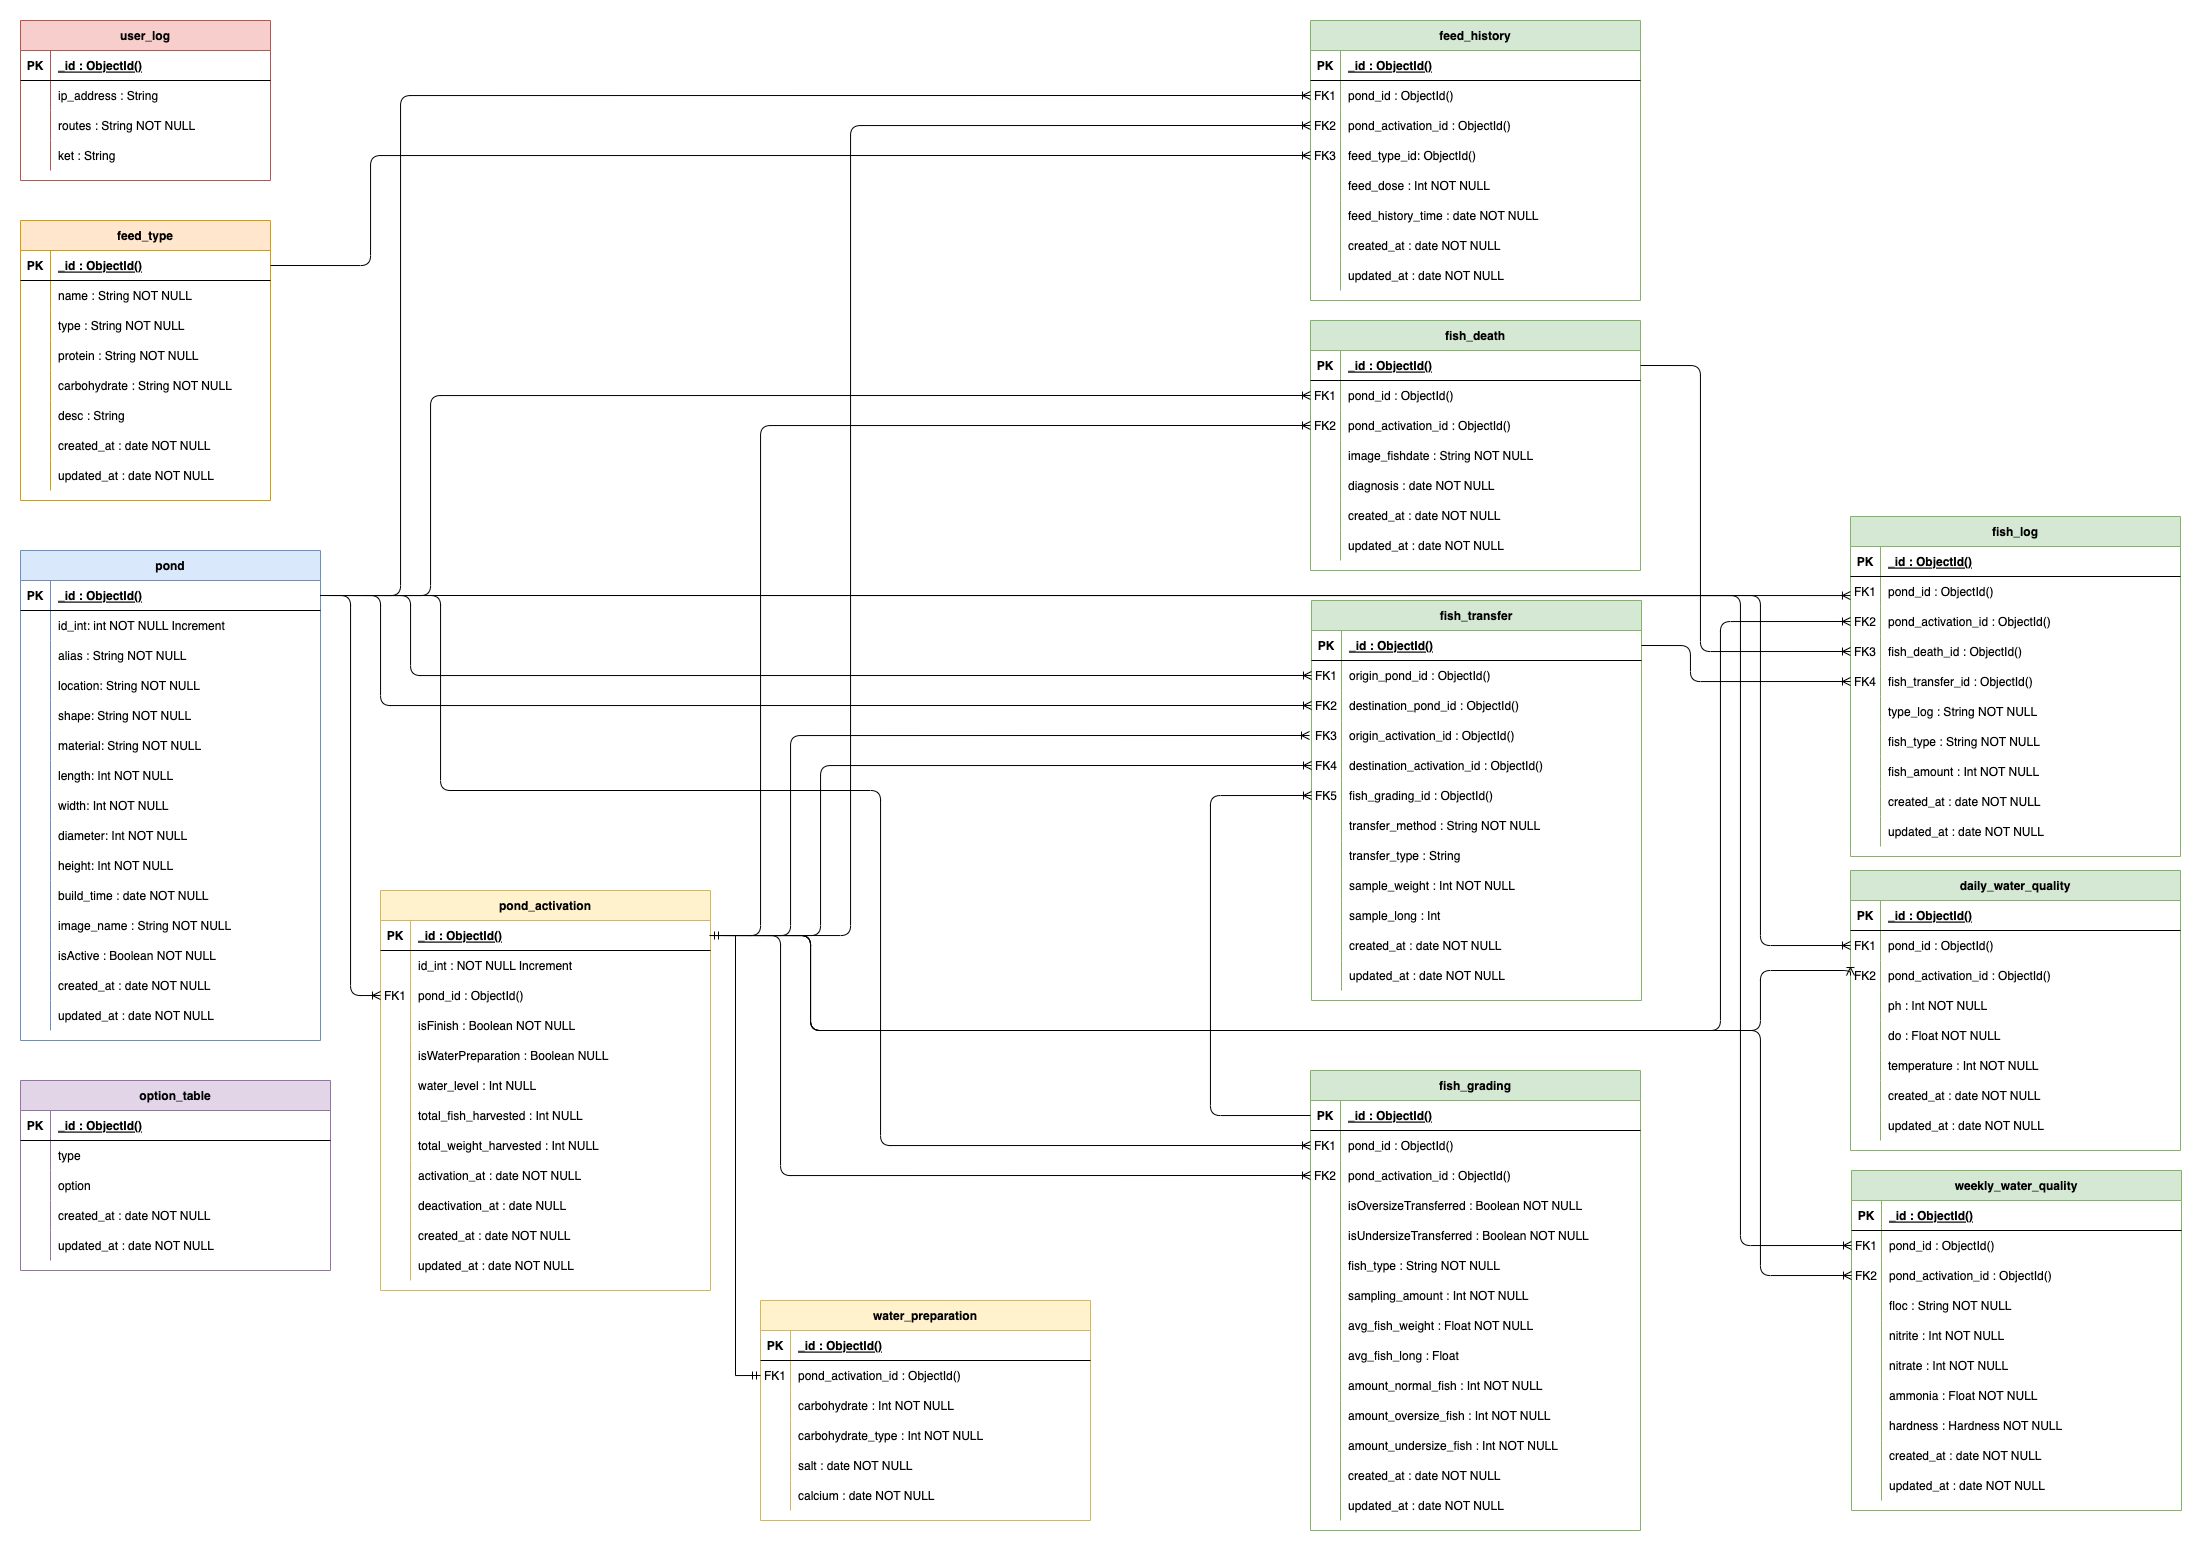
\includegraphics[height=0.7\textwidth]{gambar/Sprint09/diagram database/database}
	\caption{ERD Database Sprint-9}
	\label{fig:database_sprint9}
\end{figure}

Dengan berubahnya desain database diperlukan juga penambahan model pada source code, berikut perubahan pada source code model.

\begin{lstlisting}
# fishapi/database/model.py

class DailyWaterQuality(db.Document):
    pond_id = db.ReferenceField(Pond, required=True)
    pond_activation_id = db.ReferenceField(PondActivation, required=True)
    ph = db.IntField(required=True)
    do = db.FloatField(required=True)
    temperature = db.IntField(required=True)
    created_at = db.DateTimeField(default=datetime.datetime.now)
    updated_at = db.DateTimeField(default=datetime.datetime.now)


class WeeklyWaterQuality(db.Document):
    floc_option = ('0-10', '11-30', '31-50', '51-100', '101-300', '>300')
    nitrite_option = (0, 1, 5, 10, 20, 40, 80)
    nitrate_option = (0, 10, 25, 50, 100, 250, 500)
    ammonia_option = (0, 0.25, 1.5, 3, 5)
    hardness_option = (0, 25, 50, 125, 250, 425)

    pond_id = db.ReferenceField(Pond, required=True)
    pond_activation_id = db.ReferenceField(PondActivation, required=True)
    floc = db.StringField(required=True, choices=floc_option)
    nitrite = db.IntField(required=True, choices=nitrite_option)
    nitrate = db.IntField(required=True, choices=nitrate_option)
    ammonia = db.FloatField(required=True, choices=ammonia_option)
    hardness = db.IntField(required=True, choices=hardness_option)
    created_at = db.DateTimeField(default=datetime.datetime.now)
    updated_at = db.DateTimeField(default=datetime.datetime.now)
\end{lstlisting}



\item \textbf{Menambahkan routes API}

\begin{lstlisting}
# fishapi/resource/routes.py

# daily water
    api.add_resource(DailyWaterQualitysApi, '/api/dailywaterquality')
    api.add_resource(DailyWaterQualityApi, '/api/dailywaterquality/<id>')

    # weekly water
    api.add_resource(WeeklyWaterQualitysApi, '/api/weeklywaterquality')
    api.add_resource(WeeklyWaterQualityApi, '/api/weeklywaterquality/<id>')
\end{lstlisting}




\item \textbf{Implementasi controller entry pencatatan kualitas kolam harian}

Implementasi controller API entry pencatatan kualitas kolam harian, berikut merupakan perubahan source code controller API entry pencatatan kualitas kolam harian.

\begin{lstlisting}
# fishapi/resource/dailywaterquality.py

class DailyWaterQualitysApi(Resource):
    def post(self):
        try:
            pond_id = request.form.get("pond_id", None)
            pond = Pond.objects.get(id=pond_id)
            if pond['isActive'] == False:
                response = {"message": "pond is not active"}
                response = json.dumps(response, default=str)
                return Response(response, mimetype="application/json", status=400)
            pond_activation = PondActivation.objects(
                pond_id=pond_id, isFinish=False).order_by('-activated_at').first()
            body = {
                "pond_id": pond.id,
                "pond_activation_id": pond_activation.id,
                "ph": request.form.get("ph", None),
                "do": request.form.get("do", None),
                "temperature": request.form.get("temperature", None),
            }
            print(body)
            dailywaterquality = DailyWaterQuality(**body).save()
            id = dailywaterquality.id
            response = {
                "message": "success add data daily water quality", "id": id}
            response = json.dumps(response, default=str)
            return Response(response, mimetype="application/json", status=200)
        except Exception as e:
            response = {"message": str(e)}
            response = json.dumps(response, default=str)
            return Response(response, mimetype="application/json", status=400)
\end{lstlisting}


Kode di atas merupakan implementasi sebuah API endpoint dengan kelas DailyWaterQualitysApi. Kode tersebut berfungsi untuk menangani permintaan HTTP POST yang diterima pada endpoint tersebut. Berikut adalah penjelasan langkah-langkah yang dilakukan oleh kode tersebut:

\begin{enumerate}
\item Metode post() digunakan untuk menangani permintaan POST pada endpoint DailyWaterQualitysApi.
\item Di dalam blok try, pertama-tama dilakukan pengambilan nilai pond\_id dari data form yang dikirim dalam permintaan.
\item Kemudian, dilakukan pencarian objek Pond berdasarkan pond\_id yang diperoleh.
\item Jika nilai isActive pada objek Pond adalah False, artinya kolam tidak aktif, maka akan mengembalikan respons dengan pesan error yang sesuai.
\item Selanjutnya, dilakukan pencarian objek PondActivation terbaru (dengan isFinish bernilai False) berdasarkan pond\_id yang diperoleh, dengan urutan berdasarkan activated\_at secara menurun.
\item Data yang diperoleh dari form dan informasi kolam dan aktivasi yang ditemukan digabungkan ke dalam variabel body.
\item Objek DailyWaterQuality baru dibuat dengan menggunakan nilai-nilai dari body dan kemudian disimpan ke database dengan menggunakan metode .save(). Hasilnya akan disimpan dalam variabel dailywaterquality.
\item Dari objek dailywaterquality, diambil nilai id dan disimpan dalam variabel id.
\item Hasil akhir yang akan dikembalikan sebagai respons adalah pesan sukses beserta id dari data yang berhasil ditambahkan dalam format JSON.
\item Jika terjadi exception atau kesalahan, akan di-handle dengan mengembalikan respons dengan pesan error yang sesuai dalam format JSON dan status kode 400.
\end{enumerate}
Dengan demikian, kode tersebut mengimplementasikan logika untuk menambahkan data kualitas air harian (DailyWaterQuality) ke dalam database berdasarkan permintaan POST yang diterima.

Berikut merupakan form untuk entry pencatatan kualitas kolam harian.

\begin{longtable}{| l | p{5cm} | p{5cm} |}
\caption{Form entry pencatatan kolam harian.\label{table:form_entry_pencatatan_kolam_harian}}\\

\hline
\multicolumn{1}{|c|}{\textbf{Form}} & \multicolumn{1}{|c|}{\textbf{Jenis Data}} & \multicolumn{1}{|c|}{\textbf{Deskripsi}}\\
\hline
\endfirsthead

\hline
\multicolumn{3}{|c|}{Lanjutan Tabel \ref{table:form_entry_pencatatan_kolam_harian}}\\
\hline
\multicolumn{1}{|c|}{\textbf{Form}} & \multicolumn{1}{|c|}{\textbf{Jenis Data}} & \multicolumn{1}{|c|}{\textbf{Deskripsi}}\\
\hline
\endhead

                                          

pond\_id   & REQUIRED STRING & id kolam yang akan di lakukan pencatatan kualitas air harian \\ \hline
ph         & REQUIRED INT    & tingkat ph air satuan (pH)                                   \\ \hline
do         & REQUIRED INT    & oksigen yang terlarut dalam air (ppm)                        \\ \hline
temprature & REQUIRED INT    & suhu air kolam (\textdegree C)                \\ \hline
\end{longtable}



Tabel di atas menggambarkan struktur data yang diperlukan untuk melakukan pencatatan kualitas air harian dalam kolam. Berikut adalah penjelasan untuk setiap kolom dalam tabel:

\begin{enumerate}

\item pond\_id: Kolom ini merupakan string yang wajib diisi. Nilai yang dimasukkan adalah ID kolam yang akan dicatat kualitas air hariannya. Kolom ini digunakan untuk mengaitkan catatan kualitas air dengan kolam yang sesuai.

\item ph: Kolom ini merupakan integer yang wajib diisi. Nilai yang dimasukkan adalah tingkat pH air dalam satuan pH (potensi hidrogen). pH mengindikasikan tingkat keasaman atau kebasaan air. Pengukuran ini penting karena kualitas air yang baik untuk ikan seringkali terkait dengan tingkat pH yang sesuai.

\item do: Kolom ini merupakan integer yang wajib diisi. Nilai yang dimasukkan adalah tingkat oksigen terlarut dalam air dalam satuan ppm (parts per million). Oksigen terlarut penting untuk kelangsungan hidup ikan dan organisme akuatik lainnya. Pemantauan kadar oksigen terlarut membantu memastikan bahwa lingkungan air di dalam kolam memadai bagi ikan.

\item temperature: Kolom ini merupakan integer yang wajib diisi. Nilai yang dimasukkan adalah suhu air kolam dalam satuan derajat Celsius. Suhu air mempengaruhi kesehatan dan pertumbuhan ikan. Pengukuran suhu air membantu memantau perubahan suhu yang dapat memengaruhi kondisi ikan dan keseimbangan ekosistem di dalam kolam.

\end{enumerate}

Dengan menggunakan struktur data yang terdefinisi dalam tabel ini, pengguna dapat mencatat kualitas air harian dengan mengisi nilai-nilai yang sesuai untuk setiap kolom. Data ini penting untuk pemantauan dan pengelolaan yang efektif dalam budidaya ikan, serta untuk menjaga kesehatan dan kualitas lingkungan air di dalam kolam.


Berikut merupakan hasil test request dari API entry pencatatan kolam harian.

cURL:

\begin{lstlisting}
curl --location 'http://jft.web.id/fishapi/api/dailywaterquality' \
--form 'pond_id="{pond_id}"' \
--form 'ph="1"' \
--form 'do="6"' \
--form 'temperature="20"'
\end{lstlisting}

response json:

\begin{lstlisting}
{
  "message": "success add data daily water quality",
  "id": "62e8b800ef4edacc5bb18b05"
}
\end{lstlisting}




\item \textbf{Implementasi API fetch list pencatatan kolam harian}

Implementasi controller API fetch list pencatatan kolam harian, berikut merupakan source code controller API fetch list pencatatan kolam harian.

\begin{lstlisting}
# fishapi/resource/dailywaterquality.py

class DailyWaterQualitysApi(Resource):
    def get(self):
        try:
            pipeline = [
                {"$sort": {"created_at": -1}},
                {'$lookup': {
                    'from': 'pond',
                    'let': {"pondid": "$pond_id"},
                    'pipeline': [
                        {'$match': {'$expr': {'$eq': ['$_id', '$$pondid']}}},
                        {"$project": {
                            "_id": 1,
                            "alias": 1,
                            "location": 1,
                            "build_at": 1,
                            "isActive": 1,
                        }}
                    ],
                    'as': 'pond'
                }},
                {'$lookup': {
                    'from': 'pond_activation',
                    'let': {"activationid": "$pond_activation_id"},
                    'pipeline': [
                        {'$match': {
                            '$expr': {'$eq': ['$_id', '$$activationid']}}},
                        {"$project": {
                            "_id": 1,
                            "isFinish": 1,
                            "isWaterPreparation": 1,
                            "water_level": 1,
                            "activated_at": 1
                        }}
                    ],
                    'as': 'pond_activation'
                }},
                {"$addFields": {
                    "pond": {"$first": "$pond"},
                    "pond_activation": {"$first": "$pond_activation"},
                    "ph_desc": {
                        "$switch":
                            {
                                "branches": [
                                    {
                                        "case": {"$lt": ["$ph", 6]},
                                        "then": "berbahaya"
                                    },
                                    {
                                        "case": {"$gt": ["$ph", 8]},
                                        "then": "berbahaya"
                                    }
                                ],
                                "default": "normal"
                            }
                    },
                    "do_desc": {
                        "$switch":
                            {
                                "branches": [
                                    {
                                        "case": {"$or": [
                                            {"$lt": ["$do", 3]},
                                            {"$gt": ["$do", 7.5]}
                                        ]},
                                        "then": "berbahaya"
                                    },
                                    {
                                        "case": {"$or": [
                                            {"$and": [{"$gte": ["$do", 3]}, {
                                                "$lte": ["$do", 4]}]},
                                            {"$and": [{"$gt": ["$do", 6]}, {
                                                "$lte": ["$do", 7.5]}]}
                                        ]},
                                        "then": "semi berbahaya"
                                    }
                                ],
                                "default": "normal"
                            }
                    }
                }},
                {"$project": {
                    "updated_at": 0,
                    "created_at": 0,
                }}
            ]
            dailywaterquality = DailyWaterQuality.objects.aggregate(pipeline)
            list_dailywaterqualitys = list(dailywaterquality)
            response = json.dumps(list_dailywaterqualitys, default=str)
            return Response(response, mimetype="application/json", status=200)
        except Exception as e:
            response = {"message": str(e)}
            response = json.dumps(response, default=str)
            return Response(response, mimetype="application/json", status=400)
\end{lstlisting}


Kode di atas merupakan implementasi dari sebuah API dengan nama DailyWaterQualitysApi yang bertujuan untuk mengambil data kualitas air harian (DailyWaterQuality). Berikut penjelasan tentang kode tersebut:

API ini menyediakan metode get() yang digunakan untuk mengambil data kualitas air harian. Dalam metode tersebut, dilakukan serangkaian operasi pengolahan data menggunakan Aggregation Framework pada MongoDB.

Pertama, sebuah pipeline dibuat sebagai langkah-langkah pengolahan data. Pada langkah awal, data diurutkan berdasarkan waktu pembuatan (created\_at) secara menurun (descending) menggunakan operasi \$sort.

Selanjutnya, dilakukan operasi \$lookup untuk melakukan join dengan dua koleksi lain, yaitu "pond" dan "pond\_activation". Dalam langkah ini, dilakukan pencocokan (\$match) berdasarkan nilai \_id pada koleksi "pond" dan "pond\_activation" dengan nilai yang berasal dari koleksi "DailyWaterQuality". Hasil join disimpan dalam array pond dan pond\_activation.

Setelah itu, dilakukan penambahan kolom baru (\$addFields) pada dokumen dengan menggunakan hasil join sebelumnya. Kolom baru yang ditambahkan antara lain pond (berisi data kolam yang terkait), pond\_activation (berisi data aktivasi kolam yang terkait), ph\_desc (deskripsi tingkat pH), dan do\_desc (deskripsi tingkat oksigen terlarut). Deskripsi tersebut ditentukan berdasarkan kondisi yang didefinisikan dengan operator \$switch.

Langkah terakhir dalam pipeline adalah menggunakan operasi \$project untuk menghilangkan kolom updated\_at dan created\_at dari hasil akhir.

Setelah pipeline selesai, dilakukan agregasi pada koleksi "DailyWaterQuality" menggunakan pipeline yang telah dibuat. Hasil agregasi kemudian diubah menjadi list dan dikonversi menjadi format JSON. Respon JSON ini kemudian dikembalikan sebagai respons dari API dengan kode status 200 (OK).

Namun, jika terjadi kesalahan selama proses, dilakukan penanganan eksepsi (exception) yang menghasilkan pesan error. Pesan error tersebut kemudian dikonversi menjadi format JSON dan dikembalikan sebagai respons dari API dengan kode status 400 (Bad Request).

Berikut merupakan hasil test request dari API fetch list pencatatan kolam harian.

cURL:

\begin{lstlisting}
curl --location 'http://jft.web.id/fishapi/api/dailywaterquality'
\end{lstlisting}

response json:

\begin{lstlisting}
[
    {
        "_id": "647edbe028aa8efac0b6c2f2",
        "pond_id": "647d8beb28aa8efac0b6c2ed",
        "pond_activation_id": "647d8c0b28aa8efac0b6c2ee",
        "ph": 1,
        "do": 6.0,
        "temperature": 20,
        "pond": {
            "_id": "647d8beb28aa8efac0b6c2ed",
            "alias": "charlie",
            "location": "blok 3",
            "isActive": true,
            "build_at": "2023-06-05 14:16:59.384000"
        },
        "pond_activation": {
            "_id": "647d8c0b28aa8efac0b6c2ee",
            "isFinish": false,
            "isWaterPreparation": false,
            "water_level": 100.0,
            "activated_at": "2023-06-05 14:17:31.973000"
        },
        "ph_desc": "berbahaya",
        "do_desc": "normal"
    },
    {
        "_id": "647edbe028aa8efac0b6c2f2",
        "pond_id": "647d8beb28aa8efac0b6c2ed",
        "pond_activation_id": "647d8c0b28aa8efac0b6c2ee",
        "ph": 1,
        "do": 6.0,
        "temperature": 20,
        "pond": {
            "_id": "647d8beb28aa8efac0b6c2ed",
            "alias": "charlie",
            "location": "blok 3",
            "isActive": true,
            "build_at": "2023-06-05 14:16:59.384000"
        },
        "pond_activation": {
            "_id": "647d8c0b28aa8efac0b6c2ee",
            "isFinish": false,
            "isWaterPreparation": false,
            "water_level": 100.0,
            "activated_at": "2023-06-05 14:17:31.973000"
        },
        "ph_desc": "berbahaya",
        "do_desc": "normal"
    }
]
\end{lstlisting}



\item \textbf{Implementasi API edit pencatatan kolam harian}

Implementasi controller API edit pencatatan kolam harian, berikut merupakan perubahan source code controller API edit pencatatan kolam harian.

\begin{lstlisting}
# fishapi/database/dailywaterquality.py

class DailyWaterQualityApi(Resource):
    def put(self, id):
        try:
            body = request.form.to_dict(flat=True)
            DailyWaterQuality.objects.get(id=id).update(**body)
            response = {
                "message": "success change data daily water quality", "id": id}
            response = json.dumps(response, default=str)
            return Response(response, mimetype="application/json", status=200)
        except Exception as e:
            response = {"message": str(e)}
            response = json.dumps(response, default=str)
            return Response(response, mimetype="application/json", status=400)
\end{lstlisting}

Kode di atas merupakan implementasi dari sebuah API dengan nama DailyWaterQualityApi yang bertujuan untuk mengubah (update) data kualitas air harian (DailyWaterQuality) berdasarkan ID tertentu. Berikut adalah penjelasan tentang kode tersebut:

API ini menyediakan metode put() yang digunakan untuk mengubah data kualitas air harian. Metode ini menerima parameter id yang merupakan ID dari data yang akan diubah.

Dalam metode put(), terdapat beberapa langkah yang dilakukan. Pertama, nilai dari form request diubah menjadi bentuk dictionary menggunakan fungsi request.form.to\_dict(flat=True). Dictionary ini akan berisi data yang dikirimkan dalam form request.

Selanjutnya, dilakukan operasi update() pada objek DailyWaterQuality dengan menggunakan ID yang diberikan. Operasi update() ini akan memperbarui data dengan nilai-nilai yang terdapat dalam dictionary body. Data yang diubah akan sesuai dengan kolom-kolom yang ada dalam objek DailyWaterQuality.

Setelah proses pembaruan selesai, dibuat respons yang akan dikirimkan kembali kepada pengguna. Respons ini berupa pesan sukses yang mengindikasikan bahwa data kualitas air harian telah berhasil diubah. Respons tersebut juga mencakup ID dari data yang telah diubah. Pesan dan ID tersebut kemudian diubah menjadi format JSON menggunakan fungsi json.dumps().

Apabila terjadi kesalahan selama proses pembaruan, penanganan eksepsi (exception handling) akan terjadi. Pesan error yang dihasilkan akan dikonversi menjadi format JSON dan dikirimkan sebagai respons dengan kode status 400 (Bad Request).

Dengan demikian, melalui API ini pengguna dapat mengirimkan permintaan untuk mengubah data kualitas air harian berdasarkan ID tertentu, dan akan menerima respons yang mengindikasikan keberhasilan atau kegagalan pembaruan data.

Berikut merupakan hasil test request dari API edit pencatatan kolam harian.

cURL:

\begin{lstlisting}
curl --location --request PUT 'http://jft.web.id/fishapi/api/dailywaterquality/62e89ce7846724c2d2984687' \
--form 'ph="2"' \
--form 'do="7"' \
--form 'temperature="20"'
\end{lstlisting}

response json:

\begin{lstlisting}
{
  "message": "success change data daily water quality",
  "id": "62e89ce7846724c2d2984687"
}
\end{lstlisting}



\item \textbf{Implementasi API delete pencatatan kolam harian}

Implementasi controller API delete pencatatan kolam harian, berikut merupakan perubahan source code controller API delete pencatatan kolam harian.

\begin{lstlisting}
# fishapi/database/dailywaterquality.py

class DailyWaterQualityApi(Resource):
    def delete(self, id):
        try:
            dailywaterquality = DailyWaterQuality.objects.get(id=id).delete()
            response = {"message": "success delete daily water quality"}
            response = json.dumps(response, default=str)
            return Response(response, mimetype="application/json", status=200)
        except Exception as e:
            response = {"message": str(e)}
            response = json.dumps(response, default=str)
            return Response(response, mimetype="application/json", status=400)
\end{lstlisting}


API ini menyediakan metode delete() yang digunakan untuk menghapus data kualitas air harian. Metode ini menerima parameter id yang merupakan ID dari data yang akan dihapus.

Dalam metode delete(), terdapat beberapa langkah yang dilakukan. Pertama, dilakukan pengambilan objek DailyWaterQuality berdasarkan ID yang diberikan menggunakan metode get(). Kemudian, dilakukan operasi delete() pada objek tersebut untuk menghapus data dari koleksi.

Setelah proses penghapusan selesai, dibuat respons yang akan dikirimkan kembali kepada pengguna. Respons ini berupa pesan sukses yang mengindikasikan bahwa data kualitas air harian telah berhasil dihapus. Pesan tersebut kemudian diubah menjadi format JSON menggunakan fungsi json.dumps().

Apabila terjadi kesalahan selama proses penghapusan, penanganan eksepsi (exception handling) akan terjadi. Pesan error yang dihasilkan akan dikonversi menjadi format JSON dan dikirimkan sebagai respons dengan kode status 400 (Bad Request).

Dengan demikian, melalui API ini pengguna dapat mengirimkan permintaan untuk menghapus data kualitas air harian berdasarkan ID tertentu, dan akan menerima respons yang mengindikasikan keberhasilan atau kegagalan penghapusan data.

Berikut merupakan hasil test request dari API delete pencatatan kolam harian.

cURL:

\begin{lstlisting}
curl --location --request DELETE 'http://jft.web.id/fishapi/api/dailywaterquality/62e8b800ef4edacc5bb18b05'
\end{lstlisting}

response json:

\begin{lstlisting}
{
  "message": "success delete daily water quality"
}
\end{lstlisting}


\item \textbf{Implementasi API fetch detail pencatatan kolam harian dengan id}

Implementasi controller API fetch detail pencatatan kolam harian, berikut merupakan source code controller API fetch detail pencatatan kolam harian.

\begin{lstlisting}
# fishapi/resource/dailywaterquality.py

class DailyWaterQualityApi(Resource):
    def get(self, id):
        try:
            pipeline = [
                {'$match': {'$expr': {'$eq': ['$_id', {'$toObjectId': id}]}}},
                {'$lookup': {
                    'from': 'pond',
                    'let': {"pondid": "$pond_id"},
                    'pipeline': [
                        {'$match': {'$expr': {'$eq': ['$_id', '$$pondid']}}},
                        {"$project": {
                            "_id": 1,
                            "alias": 1,
                            "location": 1,
                            "build_at": 1,
                            "isActive": 1,
                        }}
                    ],
                    'as': 'pond'
                }},
                {'$lookup': {
                    'from': 'pond_activation',
                    'let': {"activationid": "$pond_activation_id"},
                    'pipeline': [
                        {'$match': {
                            '$expr': {'$eq': ['$_id', '$$activationid']}}},
                        {"$project": {
                            "_id": 1,
                            "isFinish": 1,
                            "isWaterPreparation": 1,
                            "water_level": 1,
                            "activated_at": 1
                        }}
                    ],
                    'as': 'pond_activation'
                }},
                {"$addFields": {
                    "pond": {"$first": "$pond"},
                    "pond_activation": {"$first": "$pond_activation"},
                    "ph_desc": {
                        "$switch":
                            {
                                "branches": [
                                    {
                                        "case": {"$lt": ["$ph", 6]},
                                        "then": "berbahaya"
                                    },
                                    {
                                        "case": {"$gt": ["$ph", 8]},
                                        "then": "berbahaya"
                                    }
                                ],
                                "default": "normal"
                            }
                    },
                    "do_desc": {
                        "$switch":
                            {
                                "branches": [
                                    {
                                        "case": {"$or": [
                                            {"$lt": ["$do", 3]},
                                            {"$gt": ["$do", 7.5]}
                                        ]},
                                        "then": "berbahaya"
                                    },
                                    {
                                        "case": {"$or": [
                                            {"$and": [{"$gte": ["$do", 3]}, {
                                                "$lte": ["$do", 4]}]},
                                            {"$and": [{"$gt": ["$do", 6]}, {
                                                "$lte": ["$do", 7.5]}]}
                                        ]},
                                        "then": "semi berbahaya"
                                    }
                                ],
                                "default": "normal"
                            }
                    }
                }},
                {"$project": {
                    "updated_at": 0,
                    "created_at": 0,
                }}
            ]
            dailywaterquality = DailyWaterQuality.objects.aggregate(pipeline)
            list_dailywaterqualitys = list(dailywaterquality)
            response = json.dumps(list_dailywaterqualitys[0], default=str)
            return Response(response, mimetype="application/json", status=200)
        except Exception as e:
            response = {"message": str(e)}
            response = json.dumps(response, default=str)
            return Response(response, mimetype="application/json", status=400)
\end{lstlisting}


Kode di atas merupakan implementasi dari sebuah API dengan nama DailyWaterQualityApi yang digunakan untuk mendapatkan (get) data kualitas air harian (DailyWaterQuality) berdasarkan ID tertentu. Berikut adalah penjelasan tentang kode tersebut:

API ini menyediakan metode get() yang digunakan untuk mengambil data kualitas air harian berdasarkan ID. Metode ini menerima parameter id yang merupakan ID dari data yang akan diambil.

Dalam metode get(), terdapat beberapa langkah yang dilakukan. Pertama, terdapat penggunaan pipeline yang berisi serangkaian tahapan untuk melakukan agregasi dan pencarian data menggunakan MongoDB. Tahapan-tahapan tersebut meliputi pencocokan (\$match) berdasarkan ID yang diberikan, pencarian relasi dengan koleksi pond dan pond\_activation menggunakan \$lookup, dan penambahan (\$addFields) beberapa field baru ke hasil agregasi.

Beberapa field baru yang ditambahkan adalah ph\_desc dan do\_desc, yang bergantung pada nilai ph dan do pada data kualitas air harian. Nilai-nilai tersebut diuji menggunakan operator \$switch untuk menentukan deskripsi kualitas air berdasarkan batasan-batasan tertentu.

Setelah tahapan agregasi selesai, hasil aggregasi tersebut dikonversi menjadi daftar (list) dan diambil elemen pertama (list\_dailywaterqualitys[0]). Hasil tersebut kemudian diubah menjadi format JSON menggunakan fungsi json.dumps().

Apabila terjadi kesalahan selama proses pengambilan data, penanganan eksepsi (exception handling) akan terjadi. Pesan error yang dihasilkan akan dikonversi menjadi format JSON dan dikirimkan sebagai respons dengan kode status 400 (Bad Request).


Berikut merupakan hasil test request dari API fetch pencatatan kolam harian berdasarkan id.

cURL:

\begin{lstlisting}
curl --location 'http://jft.web.id/fishapi/api/dailywaterquality/62e89ce7846724c2d2984687'
\end{lstlisting}

response json:

\begin{lstlisting}
{
  "_id": "62e89ce7846724c2d2984687",
  "pond_id": "62a62163e445ffb9c5f746f3",
  "pond_activation_id": "62d3f2180d7265ab60f9cb83",
  "ph": 7,
  "do": 4,
  "temperature": 25,
  "pond": {
    "_id": "62a62163e445ffb9c5f746f3",
    "alias": "charlie",
    "location": "blok 2",
    "build_at": "2022-06-13 00:24:51.473000",
    "isActive": true
  },
  "pond_activation": {
    "_id": "62d3f2180d7265ab60f9cb83",
    "isFinish": false,
    "isWaterPreparation": true,
    "water_level": 100,
    "activated_at": "2022-07-17 18:27:20.511000"
  },
  "ph_desc": "normal",
  "do_desc": "semi berbahaya"
}
\end{lstlisting}




\item \textbf{Implementasi controller entry pencatatan kualitas kolam mingguan}

Implementasi controller API entry pencatatan kualitas kolam mingguan, berikut merupakan perubahan source code controller API entry pencatatan kualitas kolam mingguan.

\begin{lstlisting}
# fishapi/resource/weeklywaterquality.py

class WeeklyWaterQualitysApi(Resource):
    def post(self):
        try:
            pond_id = request.form.get("pond_id", None)
            pond = Pond.objects.get(id=pond_id)
            if pond['isActive'] == False:
                response = {"message": "pond is not active"}
                response = json.dumps(response, default=str)
                return Response(response, mimetype="application/json", status=400)
            pond_activation = PondActivation.objects(
                pond_id=pond_id, isFinish=False).order_by('-activated_at').first()
            body = {
                "pond_id": pond.id,
                "pond_activation_id": pond_activation.id,
                "floc": request.form.get("floc", None),
                "nitrite": request.form.get("nitrite", None),
                "nitrate": request.form.get("nitrate", None),
                "ammonia": request.form.get("ammonia", None),
                "hardness": request.form.get("hardness", None),
            }
            weeklywaterquality = WeeklyWaterQuality(**body).save()
            id = weeklywaterquality.id
            response = {
                "message": "success add data weekly water quality", "id": id}
            response = json.dumps(response, default=str)
            return Response(response, mimetype="application/json", status=200)
        except Exception as e:
            response = {"message": str(e)}
            response = json.dumps(response, default=str)
            return Response(response, mimetype="application/json", status=400)
\end{lstlisting}


Kode di atas merupakan implementasi dari sebuah API dengan nama WeeklyWaterQualitysApi. API ini digunakan untuk menambahkan (post) data kualitas air mingguan (WeeklyWaterQuality) ke dalam sistem. Berikut adalah penjelasan mengenai kode tersebut:

API ini menyediakan metode post() yang digunakan untuk menangani permintaan untuk menambahkan data kualitas air mingguan ke sistem. Metode ini menerima data yang dikirimkan dalam format form-data melalui permintaan HTTP POST.

Pertama, kode ini mengambil nilai pond\_id dari permintaan menggunakan request.form.get(). Nilai ini digunakan untuk mendapatkan objek kolam (pond) dari basis data menggunakan metode objects.get() dari model Pond. Jika kolam dengan ID tersebut tidak aktif (isActive = False), maka API akan memberikan respons dengan pesan error yang menyatakan "pond is not active".

Selanjutnya, kode ini mencari aktivasi kolam (pond\_activation) terbaru yang belum selesai (isFinish = False) berdasarkan pond\_id. Aktivasi kolam ini diurutkan berdasarkan waktu aktivasi (activated\_at) secara menurun (descending) menggunakan metode order\_by() dan diambil aktivasi pertama menggunakan first(). Informasi ini akan digunakan dalam pembuatan objek WeeklyWaterQuality.

Data untuk objek WeeklyWaterQuality, seperti floc, nitrite, nitrate, ammonia, dan hardness, diambil dari permintaan menggunakan request.form.get(). Kemudian, objek WeeklyWaterQuality baru dibuat dengan menggunakan data tersebut dan disimpan ke dalam basis data menggunakan metode save().

Setelah penyimpanan berhasil, respons sukses dengan pesan "success add data weekly water quality" dan ID objek yang baru dibuat (id) dikirimkan sebagai respons dalam format JSON.

Namun, jika terjadi kesalahan selama proses tersebut, blok except akan menangkap eksepsi yang terjadi dan memberikan respons dengan pesan error yang dihasilkan.

Dengan demikian, melalui API ini pengguna dapat mengirimkan permintaan untuk menambahkan data kualitas air mingguan ke sistem. Jika permintaan berhasil, pengguna akan menerima respons sukses dengan ID data yang baru ditambahkan. Jika terjadi kesalahan, respons error akan diberikan dengan pesan yang menjelaskan kesalahan tersebut.

Berikut merupakan form untuk entry pencatatan kualitas kolam mingguan.

\begin{longtable}{| l | p{5cm} | p{5cm} |}
\caption{Form entry pencatatan kolam mingguan.\label{table:form_entry_pencatatan_kolam_mingguan}}\\

\hline
\multicolumn{1}{|c|}{\textbf{Form}} & \multicolumn{1}{|c|}{\textbf{Jenis Data}} & \multicolumn{1}{|c|}{\textbf{Deskripsi}}\\
\hline
\endfirsthead

\hline
\multicolumn{3}{|c|}{Lanjutan Tabel \ref{table:form_entry_pencatatan_kolam_mingguan}}\\
\hline
\multicolumn{1}{|c|}{\textbf{Form}} & \multicolumn{1}{|c|}{\textbf{Jenis Data}} & \multicolumn{1}{|c|}{\textbf{Deskripsi}}\\
\hline
\endhead

                                          

pond\_id & REQUIRED STRING                                                                               & id kolam yang akan di lakukan pencatatan kualitas air mingguan \\ \hline
floc     & OPTION STRING VALUE: {[}'0-10', '11-30', '31-50', '51-100', '101-300', '\textgreater{}300'{]} & kadar floc dalam air                                           \\ \hline
nitrite  & OPTION INT VALUE: {[}0, 1, 5, 10, 20, 40, 80{]}                                               & kadar nitrite pada air                                         \\ \hline
nitrate  & OPTION INT VALUE: {[}0, 10, 25, 50, 100, 250, 500{]}                                          & kadar nitrate pada air                                         \\ \hline
ammonia  & OPTION DOUBLE VALUE: {[}0, 0.25, 1.5, 3, 5{]}                                                 & kadar ammonia pada air                                         \\ \hline
hardness & OPTION INT VALUE: {[}0, 25, 50, 125, 250, 425{]}                                              & tingkat hardness air                                           \\ \hline
\end{longtable}



Berikut adalah penjelasan mengenai setiap kolom pada tabel:

\begin{enumerate}
\item pond\_id (REQUIRED STRING): Kolom ini menyimpan ID kolam yang akan digunakan untuk mencatat kualitas air mingguan. ID kolam harus diberikan dalam format string dan merupakan data yang wajib diisi.

\item floc (OPTION STRING): Kolom ini mencatat kadar floc dalam air. Floc adalah partikel-partikel padat yang mengendap dalam air kolam. Nilai yang dapat diisikan adalah dalam bentuk string dengan pilihan nilai yang telah ditentukan, yaitu "0-10", "11-30", "31-50", "51-100", "101-300", atau "\textgreater300". Kolom ini bersifat opsional, sehingga tidak wajib diisi.

\item nitrite (OPTION INT): Kolom ini mencatat kadar nitrite pada air. Nitrite adalah senyawa nitrogen yang dapat menjadi racun bagi ikan dan organisme akuatik lainnya jika terlalu tinggi. Nilai yang dapat diisikan adalah dalam bentuk integer (bilangan bulat) dengan pilihan nilai yang telah ditentukan, yaitu 0, 1, 5, 10, 20, 40, atau 80. Kolom ini bersifat opsional, sehingga tidak wajib diisi.

\item nitrate (OPTION INT): Kolom ini mencatat kadar nitrate pada air. Nitrate adalah senyawa nitrogen yang juga dapat menjadi racun bagi ikan dan organisme akuatik jika terlalu tinggi. Nilai yang dapat diisikan adalah dalam bentuk integer dengan pilihan nilai yang telah ditentukan, yaitu 0, 10, 25, 50, 100, 250, atau 500. Kolom ini bersifat opsional, sehingga tidak wajib diisi.

\item ammonia (OPTION DOUBLE): Kolom ini mencatat kadar ammonia pada air. Ammonia adalah senyawa nitrogen beracun yang dihasilkan oleh limbah organik dalam kolam. Nilai yang dapat diisikan adalah dalam bentuk double (bilangan desimal) dengan pilihan nilai yang telah ditentukan, yaitu 0, 0.25, 1.5, 3, atau 5. Kolom ini bersifat opsional, sehingga tidak wajib diisi.

\item hardness (OPTION INT): Kolom ini mencatat tingkat kekerasan air (hardness). Kekerasan air dapat dipengaruhi oleh kandungan mineral seperti kalsium dan magnesium. Nilai yang dapat diisikan adalah dalam bentuk integer dengan pilihan nilai yang telah ditentukan, yaitu 0, 25, 50, 125, 250, atau 425. Kolom ini bersifat opsional, sehingga tidak wajib diisi.
\end{enumerate}

Tabel tersebut memberikan informasi tentang jenis data yang harus diisi dalam setiap kolom dan deskripsi singkat tentang masing-masing kolom. Data-data ini digunakan untuk mencatat kualitas air mingguan dalam kolam dan dapat digunakan untuk analisis dan pemantauan kondisi lingkungan akuatik.


Berikut merupakan hasil test request dari API entry pencatatan kolam mingguan.

cURL:

\begin{lstlisting}
curl --location 'http://jft.web.id/fishapi/api/weeklywaterquality' \
--form 'pond_id="{pond_id}"' \
--form 'floc="11-30"' \
--form 'nitrite="20"' \
--form 'nitrate="100"' \
--form 'ammonia="1.5"' \
--form 'hardness="125"'
\end{lstlisting}

response json:

\begin{lstlisting}
{
  "message": "success add data weekly water quality",
  "id": "62e92ea6602825ffd3a1d2c1"
}
\end{lstlisting}




\item \textbf{Implementasi API fetch list pencatatan kolam mingguan}

Implementasi controller API fetch list pencatatan kolam mingguan, berikut merupakan source code controller API fetch list pencatatan kolam mingguan.

\begin{lstlisting}
# fishapi/resource/weeklywaterquality.py

class WeeklyWaterQualitysApi(Resource):
    def get(self):
        try:
            pipeline = [
                {"$sort": {"created_at": -1}},
                {'$lookup': {
                    'from': 'pond',
                    'let': {"pondid": "$pond_id"},
                    'pipeline': [
                        {'$match': {'$expr': {'$eq': ['$_id', '$$pondid']}}},
                        {"$project": {
                            "_id": 1,
                            "alias": 1,
                            "location": 1,
                            "build_at": 1,
                            "isActive": 1,
                        }}
                    ],
                    'as': 'pond'
                }},
                {'$lookup': {
                    'from': 'pond_activation',
                    'let': {"activationid": "$pond_activation_id"},
                    'pipeline': [
                        {'$match': {
                            '$expr': {'$eq': ['$_id', '$$activationid']}}},
                        {"$project": {
                            "_id": 1,
                            "isFinish": 1,
                            "isWaterPreparation": 1,
                            "water_level": 1,
                            "activated_at": 1
                        }}
                    ],
                    'as': 'pond_activation'
                }},
                {"$addFields": {
                    "pond": {"$first": "$pond"},
                    "pond_activation": {"$first": "$pond_activation"},
                    "floc_desc": {
                        "$switch":
                            {
                                "branches": [
                                    {"case": {
                                        "$eq": ["$floc", "0-10"]}, "then": "pembentukan"},
                                    {"case": {
                                        "$eq": ["$floc", "11-30"]}, "then": "normal"},
                                    {"case": {
                                        "$eq": ["$floc", "31-50"]}, "then": "tebal"},
                                    {"case": {
                                        "$eq": ["$floc", "51-100"]}, "then": "abnormal"},
                                    {"case": {
                                        "$eq": ["$floc", "101-300"]}, "then": "berbahaya"},
                                    {"case": {
                                        "$eq": ["$floc", ">300"]}, "then": "deadzone"},
                                ],
                                "default": "normal"
                            }
                    },
                    "nitrite_desc": {
                        "$switch":
                            {
                                "branches": [
                                    {"case": {
                                        "$eq": ["$ammonia", 0]}, "then": "tidak ada"},
                                    {"case": {
                                        "$eq": ["$ammonia", 1]}, "then": "sedikit"},
                                    {"case": {
                                        "$eq": ["$ammonia", 5]}, "then": "aman"},
                                    {"case": {
                                        "$eq": ["$ammonia", 10]}, "then": "pekat"},
                                    {"case": {
                                        "$eq": ["$ammonia", 20]}, "then": "banyak"},
                                    {"case": {
                                        "$eq": ["$ammonia", 40]}, "then": "berbahaya"},
                                    {"case": {
                                        "$eq": ["$ammonia", 80]}, "then": "deadzone"},
                                ],
                                "default": "normal"
                            }
                    },
                    "nitrate_desc": {
                        "$switch":
                            {
                                "branches": [
                                    {"case": {
                                        "$eq": ["$ammonia", 0]}, "then": "tidak ada"},
                                    {"case": {
                                        "$eq": ["$ammonia", 10]}, "then": "sedikit"},
                                    {"case": {
                                        "$eq": ["$ammonia", 25]}, "then": "aman"},
                                    {"case": {
                                        "$eq": ["$ammonia", 50]}, "then": "pekat"},
                                    {"case": {
                                        "$eq": ["$ammonia", 100]}, "then": "banyak"},
                                    {"case": {
                                        "$eq": ["$ammonia", 250]}, "then": "berbahaya"},
                                    {"case": {
                                        "$eq": ["$ammonia", 500]}, "then": "deadzone"},
                                ],
                                "default": "normal"
                            }
                    },
                    "ammonia_desc": {
                        "$switch":
                            {
                                "branches": [
                                    {"case": {
                                        "$eq": ["$ammonia", 0]}, "then": "sedikit"},
                                    {"case": {
                                        "$eq": ["$ammonia", 0.25]}, "then": "aman"},
                                    {"case": {
                                        "$eq": ["$ammonia", 1.5]}, "then": "pekat"},
                                    {"case": {
                                        "$eq": ["$ammonia", 3]}, "then": "banyak"},
                                    {"case": {
                                        "$eq": ["$ammonia", 5]}, "then": "berbahaya"},
                                ],
                                "default": "normal"
                            }
                    },
                    "hardness_desc": {
                        "$switch":
                            {
                                "branches": [
                                    {"case": {
                                        "$eq": ["$ammonia", 0]}, "then": "sedikit"},
                                    {"case": {
                                        "$eq": ["$ammonia", 25]}, "then": "aman"},
                                    {"case": {
                                        "$eq": ["$ammonia", 50]}, "then": "pekat"},
                                    {"case": {
                                        "$eq": ["$ammonia", 125]}, "then": "banyak"},
                                    {"case": {
                                        "$eq": ["$ammonia", 250]}, "then": "berbahaya"},
                                    {"case": {
                                        "$eq": ["$ammonia", 425]}, "then": "deadzone"},
                                ],
                                "default": "normal"
                            }
                    },
                }},
                {"$project": {
                    "updated_at": 0,
                    "created_at": 0,
                }}
            ]
            weeklywaterquality = WeeklyWaterQuality.objects.aggregate(pipeline)
            list_weeklywaterqualitys = list(weeklywaterquality)
            response = json.dumps(list_weeklywaterqualitys, default=str)
            return Response(response, mimetype="application/json", status=200)
        except Exception as e:
            response = {"message": str(e)}
            response = json.dumps(response, default=str)
            return Response(response, mimetype="application/json", status=400)
\end{lstlisting}


Kode di atas adalah implementasi dari API WeeklyWaterQualitysApi yang digunakan untuk mengambil data kualitas air mingguan dari database. Berikut adalah penjelasan mengenai kode tersebut:

\begin{enumerate}

\item Pada blok try, pertama-tama kita mendefinisikan sebuah pipeline untuk melakukan agregasi data menggunakan MongoDB Aggregation Framework. Pipeline ini terdiri dari beberapa tahap yang akan diterapkan pada data WeeklyWaterQuality.

\item Tahap pertama dalam pipeline adalah \$sort, yang digunakan untuk mengurutkan data berdasarkan kolom created\_at secara descending (urutan terbalik), sehingga data terbaru akan muncul di bagian atas.

\item Tahap selanjutnya adalah \$lookup. Di sini dilakukan operasi join dengan koleksi pond dan pond\_activation. Pada \$lookup pertama, kita melakukan join dengan koleksi pond menggunakan kolom pond\_id dari WeeklyWaterQuality dan \_id dari pond. Hasil join ini akan disimpan dalam field pond pada dokumen WeeklyWaterQuality. \$lookup kedua dilakukan dengan koleksi pond\_activation menggunakan kolom pond\_activation\_id dari WeeklyWaterQuality dan \_id dari pond\_activation. Hasil join ini akan disimpan dalam field pond\_activation pada dokumen WeeklyWaterQuality.

\item Setelah dilakukan join, tahap \$addFields digunakan untuk menambahkan beberapa field baru ke dokumen WeeklyWaterQuality. Field yang ditambahkan antara lain floc\_desc, nitrite\_desc, nitrate\_desc, ammonia\_desc, dan hardness\_desc. Field-field ini akan memiliki nilai berdasarkan kondisi-kondisi yang ditentukan menggunakan operator \$switch. Misalnya, pada field floc\_desc, dilakukan pengecekan nilai field floc dan kemudian menentukan nilai berdasarkan kondisi yang sesuai. Jika nilai floc adalah "0-10", maka nilai floc\_desc akan menjadi "pembentukan".

\item Tahap terakhir adalah \$project, yang digunakan untuk mengatur proyeksi output. Di sini dilakukan penghapusan field updated\_at dan created\_at dari output agar tidak ditampilkan dalam respons API.

\item Setelah selesai mengatur pipeline, kita menjalankannya menggunakan aggregate() pada objek WeeklyWaterQuality dengan parameter pipeline yang telah dibuat. Hasil aggregasi ini kemudian dikonversi menjadi list dan disimpan dalam variabel list\_weeklywaterqualitys.

\item Setelah itu, variabel list\_weeklywaterqualitys diubah menjadi format JSON menggunakan json.dumps(). Respons JSON ini kemudian dikirimkan sebagai respons API dengan status 200 jika sukses.

\item Pada blok except, jika terjadi exception, respons akan berisi pesan error yang diambil dari exception yang terjadi.

\end{enumerate}

Kode tersebut mengimplementasikan logika untuk mengambil data kualitas air mingguan dari database, melakukan operasi join dengan koleksi lain, dan melakukan transformasi pada nilai-nilai tertentu sebelum mengirimkan respons dalam format JSON.

Berikut merupakan hasil test request dari API fetch list pencatatan kolam harian.

cURL:

\begin{lstlisting}
curl --location 'http://jft.web.id/fishapi/api/weeklywaterquality'
\end{lstlisting}

response json:

\begin{lstlisting}
[
  {
    "_id": "62e92ea6602825ffd3a1d2c1",
    "pond_id": "62a62163e445ffb9c5f746f3",
    "pond_activation_id": "62d3f2180d7265ab60f9cb83",
    "floc": "11-30",
    "nitrite": 20,
    "nitrate": 100,
    "ammonia": 1.5,
    "hardness": 125,
    "pond": {
      "_id": "62a62163e445ffb9c5f746f3",
      "alias": "charlie",
      "location": "blok 2",
      "build_at": "2022-06-13 00:24:51.473000",
      "isActive": true
    },
    "pond_activation": {
      "_id": "62d3f2180d7265ab60f9cb83",
      "isFinish": false,
      "isWaterPreparation": true,
      "water_level": 100,
      "activated_at": "2022-07-17 18:27:20.511000"
    },
    "floc_desc": "normal",
    "nitrite_desc": "normal",
    "nitrate_desc": "normal",
    "ammonia_desc": "pekat",
    "hardness_desc": "normal"
  },
  {
    "_id": "62e92e4d57ca7c50fd16795b",
    "pond_id": "62a62163e445ffb9c5f746f3",
    "pond_activation_id": "62d3f2180d7265ab60f9cb83",
    "floc": "0-10",
    "nitrite": 5,
    "nitrate": 10,
    "ammonia": 3,
    "hardness": 250,
    "pond": {
      "_id": "62a62163e445ffb9c5f746f3",
      "alias": "charlie",
      "location": "blok 2",
      "build_at": "2022-06-13 00:24:51.473000",
      "isActive": true
    },
    "pond_activation": {
      "_id": "62d3f2180d7265ab60f9cb83",
      "isFinish": false,
      "isWaterPreparation": true,
      "water_level": 100,
      "activated_at": "2022-07-17 18:27:20.511000"
    },
    "floc_desc": "pembentukan",
    "nitrite_desc": "normal",
    "nitrate_desc": "normal",
    "ammonia_desc": "banyak",
    "hardness_desc": "normal"
  },
  {
    "_id": "62e8d6263019b1590982a5e8",
    "pond_id": "62a62163e445ffb9c5f746f3",
    "pond_activation_id": "62d3f2180d7265ab60f9cb83",
    "floc": "0-10",
    "nitrite": 6,
    "nitrate": 20,
    "ammonia": 345,
    "hardness": 534,
    "pond": {
      "_id": "62a62163e445ffb9c5f746f3",
      "alias": "charlie",
      "location": "blok 2",
      "build_at": "2022-06-13 00:24:51.473000",
      "isActive": true
    },
    "pond_activation": {
      "_id": "62d3f2180d7265ab60f9cb83",
      "isFinish": false,
      "isWaterPreparation": true,
      "water_level": 100,
      "activated_at": "2022-07-17 18:27:20.511000"
    },
    "floc_desc": "pembentukan",
    "nitrite_desc": "normal",
    "nitrate_desc": "normal",
    "ammonia_desc": "normal",
    "hardness_desc": "normal"
  }
]
\end{lstlisting}



\item \textbf{Implementasi API edit pencatatan kolam mingguan}

Implementasi controller API edit pencatatan kolam minggguan, berikut merupakan perubahan source code controller API edit pencatatan kolam minggguan.

\begin{lstlisting}
# fishapi/database/weeklywaterquality.py

class WeeklyWaterQualityApi(Resource):
    def put(self, id):
        try:
            body = request.form.to_dict(flat=True)
            WeeklyWaterQuality.objects.get(id=id).update(**body)
            response = {
                "message": "success change data weekly water quality", "id": id}
            response = json.dumps(response, default=str)
            return Response(response, mimetype="application/json", status=200)
        except Exception as e:
            response = {"message": str(e)}
            response = json.dumps(response, default=str)
            return Response(response, mimetype="application/json", status=400)
\end{lstlisting}



Kode di atas adalah implementasi dari API WeeklyWaterQualityApi yang digunakan untuk memperbarui data kualitas air mingguan berdasarkan ID tertentu. Berikut adalah penjelasan mengenai kode tersebut:

Pada blok try, API ini menerima ID sebagai parameter saat melakukan permintaan PUT. Permintaan tersebut digunakan untuk mengidentifikasi entitas WeeklyWaterQuality yang akan diperbarui.

Selanjutnya, kita mendapatkan body permintaan dari request.form.to\_dict(flat=True). request.form mengandung data yang dikirim dalam permintaan PUT, dan dengan menggunakan metode to\_dict(flat=True), kita mengonversi data tersebut menjadi dictionary tunggal yang berisi pasangan kunci-nilai.

Dalam langkah selanjutnya, kita menggunakan metode get() pada model WeeklyWaterQuality dengan ID yang diberikan untuk mengambil entitas yang sesuai dari database. Kemudian, kita memanggil metode update() pada entitas yang ditemukan dan memberikan argumen **body untuk memperbarui nilai-nilai kolom dengan nilai yang baru dari body permintaan.

Jika tidak terjadi kesalahan selama proses tersebut, kita mengirimkan respons berhasil dengan status 200. Respons ini berisi pesan sukses dan ID dari entitas WeeklyWaterQuality yang telah diperbarui.

Pada blok except, jika terjadi exception selama proses tersebut, kita mengirimkan respons dengan pesan error yang diambil dari exception yang terjadi, bersama dengan status 400.

Dengan demikian, kode ini mengimplementasikan logika untuk menerima permintaan PUT dengan ID sebagai parameter, mengambil data dari permintaan, dan memperbarui entitas WeeklyWaterQuality yang sesuai dengan nilai-nilai baru.

Berikut merupakan hasil test request dari API edit pencatatan kolam mingguan.

cURL:

\begin{lstlisting}
curl --location --request PUT 'http://jft.web.id/fishapi/api/weeklywaterquality/62e92ea6602825ffd3a1d2c1' \
--form 'floc="11-30"' \
--form 'nitrite="20"' \
--form 'nitrate="100"' \
--form 'ammonia="1.5"' \
--form 'hardness="250"'
\end{lstlisting}

response json:

\begin{lstlisting}
{
  "message": "success change data weekly water quality",
  "id": "62e92ea6602825ffd3a1d2c1"
}
\end{lstlisting}



\item \textbf{Implementasi API delete pencatatan kolam mingguan}

Implementasi controller API delete pencatatan kolam mingguan, berikut merupakan perubahan source code controller API delete pencatatan kolam mingguan.

\begin{lstlisting}
# fishapi/database/weeklywaterquality.py

class WeeklyWaterQualityApi(Resource):
    def delete(self, id):
        try:
            weeklywaterquality = WeeklyWaterQuality.objects.get(id=id).delete()
            response = {"message": "success delete weekly water quality"}
            response = json.dumps(response, default=str)
            return Response(response, mimetype="application/json", status=200)
        except Exception as e:
            response = {"message": str(e)}
            response = json.dumps(response, default=str)
            return Response(response, mimetype="application/json", status=400)
\end{lstlisting}


Kode di atas adalah implementasi dari API WeeklyWaterQualityApi yang digunakan untuk menghapus data kualitas air mingguan berdasarkan ID tertentu. Berikut adalah penjelasan mengenai kode tersebut:

Pada blok try, API ini menerima ID sebagai parameter saat melakukan permintaan DELETE. Permintaan tersebut digunakan untuk mengidentifikasi entitas WeeklyWaterQuality yang akan dihapus.

Selanjutnya, kita menggunakan metode get() pada model WeeklyWaterQuality dengan ID yang diberikan untuk mengambil entitas yang sesuai dari database. Kemudian, kita memanggil metode delete() pada entitas tersebut untuk menghapusnya dari database.

Jika penghapusan berhasil dan tidak terjadi kesalahan selama proses tersebut, kita mengirimkan respons berhasil dengan status 200. Respons ini berisi pesan sukses yang mengindikasikan bahwa data kualitas air mingguan telah berhasil dihapus.

Pada blok except, jika terjadi exception selama proses tersebut, kita mengirimkan respons dengan pesan error yang diambil dari exception yang terjadi, bersama dengan status 400.

Dengan demikian, kode ini mengimplementasikan logika untuk menerima permintaan DELETE dengan ID sebagai parameter, menghapus entitas WeeklyWaterQuality yang sesuai dari database, dan mengirimkan respons berhasil jika penghapusan berhasil dilakukan.

Berikut merupakan hasil test request dari API delete pencatatan kolam harian.

cURL:

\begin{lstlisting}
curl --location --request DELETE 'http://jft.web.id/fishapi/api/weeklywaterquality/62e92ea6602825ffd3a1d2c1'
\end{lstlisting}

response json:

\begin{lstlisting}
{
  "message": "success delete weekly water quality"
}
\end{lstlisting}


\item \textbf{Implementasi API fetch detail pencatatan kolam mingguan dengan id}

Implementasi controller API fetch detail pencatatan kolam mingguan, berikut merupakan source code controller API fetch detail pencatatan kolam mingguan.

\begin{lstlisting}
# fishapi/resource/weeklywaterquality.py

class WeeklyWaterQualityApi(Resource):
    def get(self, id):
        try:
            pipeline = [
                {'$match': {'$expr': {'$eq': ['$_id', {'$toObjectId': id}]}}},
                {"$sort": {"created_at": -1}},
                {'$lookup': {
                    'from': 'pond',
                    'let': {"pondid": "$pond_id"},
                    'pipeline': [
                        {'$match': {'$expr': {'$eq': ['$_id', '$$pondid']}}},
                        {"$project": {
                            "_id": 1,
                            "alias": 1,
                            "location": 1,
                            "build_at": 1,
                            "isActive": 1,
                        }}
                    ],
                    'as': 'pond'
                }},
                {'$lookup': {
                    'from': 'pond_activation',
                    'let': {"activationid": "$pond_activation_id"},
                    'pipeline': [
                        {'$match': {
                            '$expr': {'$eq': ['$_id', '$$activationid']}}},
                        {"$project": {
                            "_id": 1,
                            "isFinish": 1,
                            "isWaterPreparation": 1,
                            "water_level": 1,
                            "activated_at": 1
                        }}
                    ],
                    'as': 'pond_activation'
                }},
                {"$addFields": {
                    "pond": {"$first": "$pond"},
                    "pond_activation": {"$first": "$pond_activation"},
                    "floc_desc": {
                        "$switch":
                            {
                                "branches": [
                                    {"case": {
                                        "$eq": ["$floc", "0-10"]}, "then": "pembentukan"},
                                    {"case": {
                                        "$eq": ["$floc", "11-30"]}, "then": "normal"},
                                    {"case": {
                                        "$eq": ["$floc", "31-50"]}, "then": "tebal"},
                                    {"case": {
                                        "$eq": ["$floc", "51-100"]}, "then": "abnormal"},
                                    {"case": {
                                        "$eq": ["$floc", "101-300"]}, "then": "berbahaya"},
                                    {"case": {
                                        "$eq": ["$floc", ">300"]}, "then": "deadzone"},
                                ],
                                "default": "normal"
                            }
                    },
                    "nitrite_desc": {
                        "$switch":
                            {
                                "branches": [
                                    {"case": {
                                        "$eq": ["$ammonia", 0]}, "then": "tidak ada"},
                                    {"case": {
                                        "$eq": ["$ammonia", 1]}, "then": "sedikit"},
                                    {"case": {
                                        "$eq": ["$ammonia", 5]}, "then": "aman"},
                                    {"case": {
                                        "$eq": ["$ammonia", 10]}, "then": "pekat"},
                                    {"case": {
                                        "$eq": ["$ammonia", 20]}, "then": "banyak"},
                                    {"case": {
                                        "$eq": ["$ammonia", 40]}, "then": "berbahaya"},
                                    {"case": {
                                        "$eq": ["$ammonia", 80]}, "then": "deadzone"},
                                ],
                                "default": "normal"
                            }
                    },
                    "nitrate_desc": {
                        "$switch":
                            {
                                "branches": [
                                    {"case": {
                                        "$eq": ["$ammonia", 0]}, "then": "tidak ada"},
                                    {"case": {
                                        "$eq": ["$ammonia", 10]}, "then": "sedikit"},
                                    {"case": {
                                        "$eq": ["$ammonia", 25]}, "then": "aman"},
                                    {"case": {
                                        "$eq": ["$ammonia", 50]}, "then": "pekat"},
                                    {"case": {
                                        "$eq": ["$ammonia", 100]}, "then": "banyak"},
                                    {"case": {
                                        "$eq": ["$ammonia", 250]}, "then": "berbahaya"},
                                    {"case": {
                                        "$eq": ["$ammonia", 500]}, "then": "deadzone"},
                                ],
                                "default": "normal"
                            }
                    },
                    "ammonia_desc": {
                        "$switch":
                            {
                                "branches": [
                                    {"case": {
                                        "$eq": ["$ammonia", 0]}, "then": "sedikit"},
                                    {"case": {
                                        "$eq": ["$ammonia", 0.25]}, "then": "aman"},
                                    {"case": {
                                        "$eq": ["$ammonia", 1.5]}, "then": "pekat"},
                                    {"case": {
                                        "$eq": ["$ammonia", 3]}, "then": "banyak"},
                                    {"case": {
                                        "$eq": ["$ammonia", 5]}, "then": "berbahaya"},
                                ],
                                "default": "normal"
                            }
                    },
                    "hardness_desc": {
                        "$switch":
                            {
                                "branches": [
                                    {"case": {
                                        "$eq": ["$ammonia", 0]}, "then": "sedikit"},
                                    {"case": {
                                        "$eq": ["$ammonia", 25]}, "then": "aman"},
                                    {"case": {
                                        "$eq": ["$ammonia", 50]}, "then": "pekat"},
                                    {"case": {
                                        "$eq": ["$ammonia", 125]}, "then": "banyak"},
                                    {"case": {
                                        "$eq": ["$ammonia", 250]}, "then": "berbahaya"},
                                    {"case": {
                                        "$eq": ["$ammonia", 425]}, "then": "deadzone"},
                                ],
                                "default": "normal"
                            }
                    },
                }},
                {"$project": {
                    "updated_at": 0,
                    "created_at": 0,
                }}
            ]
            weeklywaterquality = WeeklyWaterQuality.objects.aggregate(pipeline)
            list_weeklywaterqualitys = list(weeklywaterquality)
            response = json.dumps(list_weeklywaterqualitys[0], default=str)
            return Response(response, mimetype="application/json", status=200)
        except Exception as e:
            response = {"message": str(e)}
            response = json.dumps(response, default=str)
            return Response(response, mimetype="application/json", status=400)
\end{lstlisting}


Kode di atas adalah implementasi dari API WeeklyWaterQualityApi yang digunakan untuk mengambil data kualitas air mingguan berdasarkan ID tertentu. Berikut adalah penjelasan mengenai kode tersebut:

\begin{enumerate}

\item Pada blok try, API ini menerima ID sebagai parameter saat melakukan permintaan GET. Permintaan tersebut digunakan untuk mengidentifikasi entitas WeeklyWaterQuality yang akan diambil.

\item Kemudian, kita menggunakan aggregation framework pada MongoDB untuk menghasilkan pipa (pipeline) untuk operasi pencocokan, pengurutan, dan lookup yang kompleks. Pipa ini berisi beberapa tahapan:

\begin{enumerate}
\item Pada tahap pertama, menggunakan operasi \$match untuk mencocokkan \_id dengan ID yang diberikan.
\item Pada tahap berikutnya, menggunakan operasi \$sort untuk mengurutkan data berdasarkan created\_at secara menurun.
\item Setelah itu, menggunakan operasi \$lookup untuk menggabungkan data dari koleksi "pond" berdasarkan pond\_id. Lookup ini mengambil beberapa field spesifik dari koleksi "pond" dan memasukkannya ke dalam field pond.
\item Selanjutnya, menggunakan operasi \$lookup lagi untuk menggabungkan data dari koleksi "pond\_activation" berdasarkan pond\_activation\_id. Lookup ini mengambil beberapa field spesifik dari koleksi "pond\_activation" dan memasukkannya ke dalam field pond\_activation.
\item Kemudian, menggunakan operasi \$addFields untuk menambahkan field-field baru ke dokumen, seperti floc\_desc, nitrite\_desc, nitrate\_desc, ammonia\_desc, dan hardness\_desc. Nilai-nilai field ini dihasilkan berdasarkan operasi \$switch yang memetakan nilai-nilai field awal ke nilai deskriptif yang lebih terbaca.
\item Terakhir, menggunakan operasi \$project untuk menghilangkan field updated\_at dan created\_at dari hasil akhir.
\end{enumerate}

\item Setelah menjalankan agregasi, kita mengambil hasilnya sebagai daftar objek weeklywaterquality dan mengonversinya menjadi JSON menggunakan json.dumps(). Kita kemudian mengirimkan respons dengan hasil JSON tersebut dan status 200.

\item Pada blok except, jika terjadi exception selama proses tersebut, kita mengirimkan respons dengan pesan error yang diambil dari exception yang terjadi, bersama dengan status 400.

\end{enumerate}

Dengan demikian, kode ini mengimplementasikan logika untuk menerima permintaan GET dengan ID sebagai parameter, mengambil data kualitas air mingguan yang sesuai dari database menggunakan aggregation framework, dan mengirimkan respons dengan data yang berhasil diambil jika operasi tersebut berhasil dilakukan.


Berikut merupakan hasil test request dari API fetch pencatatan kolam mingguan berdasarkan id.

cURL:

\begin{lstlisting}
curl --location 'http://jft.web.id/fishapi/api/weeklywaterquality/62e92ea6602825ffd3a1d2c1'
\end{lstlisting}

response json:

\begin{lstlisting}
{
  "_id": "62e92ea6602825ffd3a1d2c1",
  "pond_id": "62a62163e445ffb9c5f746f3",
  "pond_activation_id": "62d3f2180d7265ab60f9cb83",
  "floc": "11-30",
  "nitrite": 20,
  "nitrate": 100,
  "ammonia": 1.5,
  "hardness": 125,
  "pond": {
    "_id": "62a62163e445ffb9c5f746f3",
    "alias": "charlie",
    "location": "blok 2",
    "build_at": "2022-06-13 00:24:51.473000",
    "isActive": true
  },
  "pond_activation": {
    "_id": "62d3f2180d7265ab60f9cb83",
    "isFinish": false,
    "isWaterPreparation": true,
    "water_level": 100,
    "activated_at": "2022-07-17 18:27:20.511000"
  },
  "floc_desc": "normal",
  "nitrite_desc": "normal",
  "nitrate_desc": "normal",
  "ammonia_desc": "pekat",
  "hardness_desc": "normal"
}
\end{lstlisting}

\item \textbf{Membuat view rekap pencatatan kolam harian}
\begin{figure}[H]
	\centering
	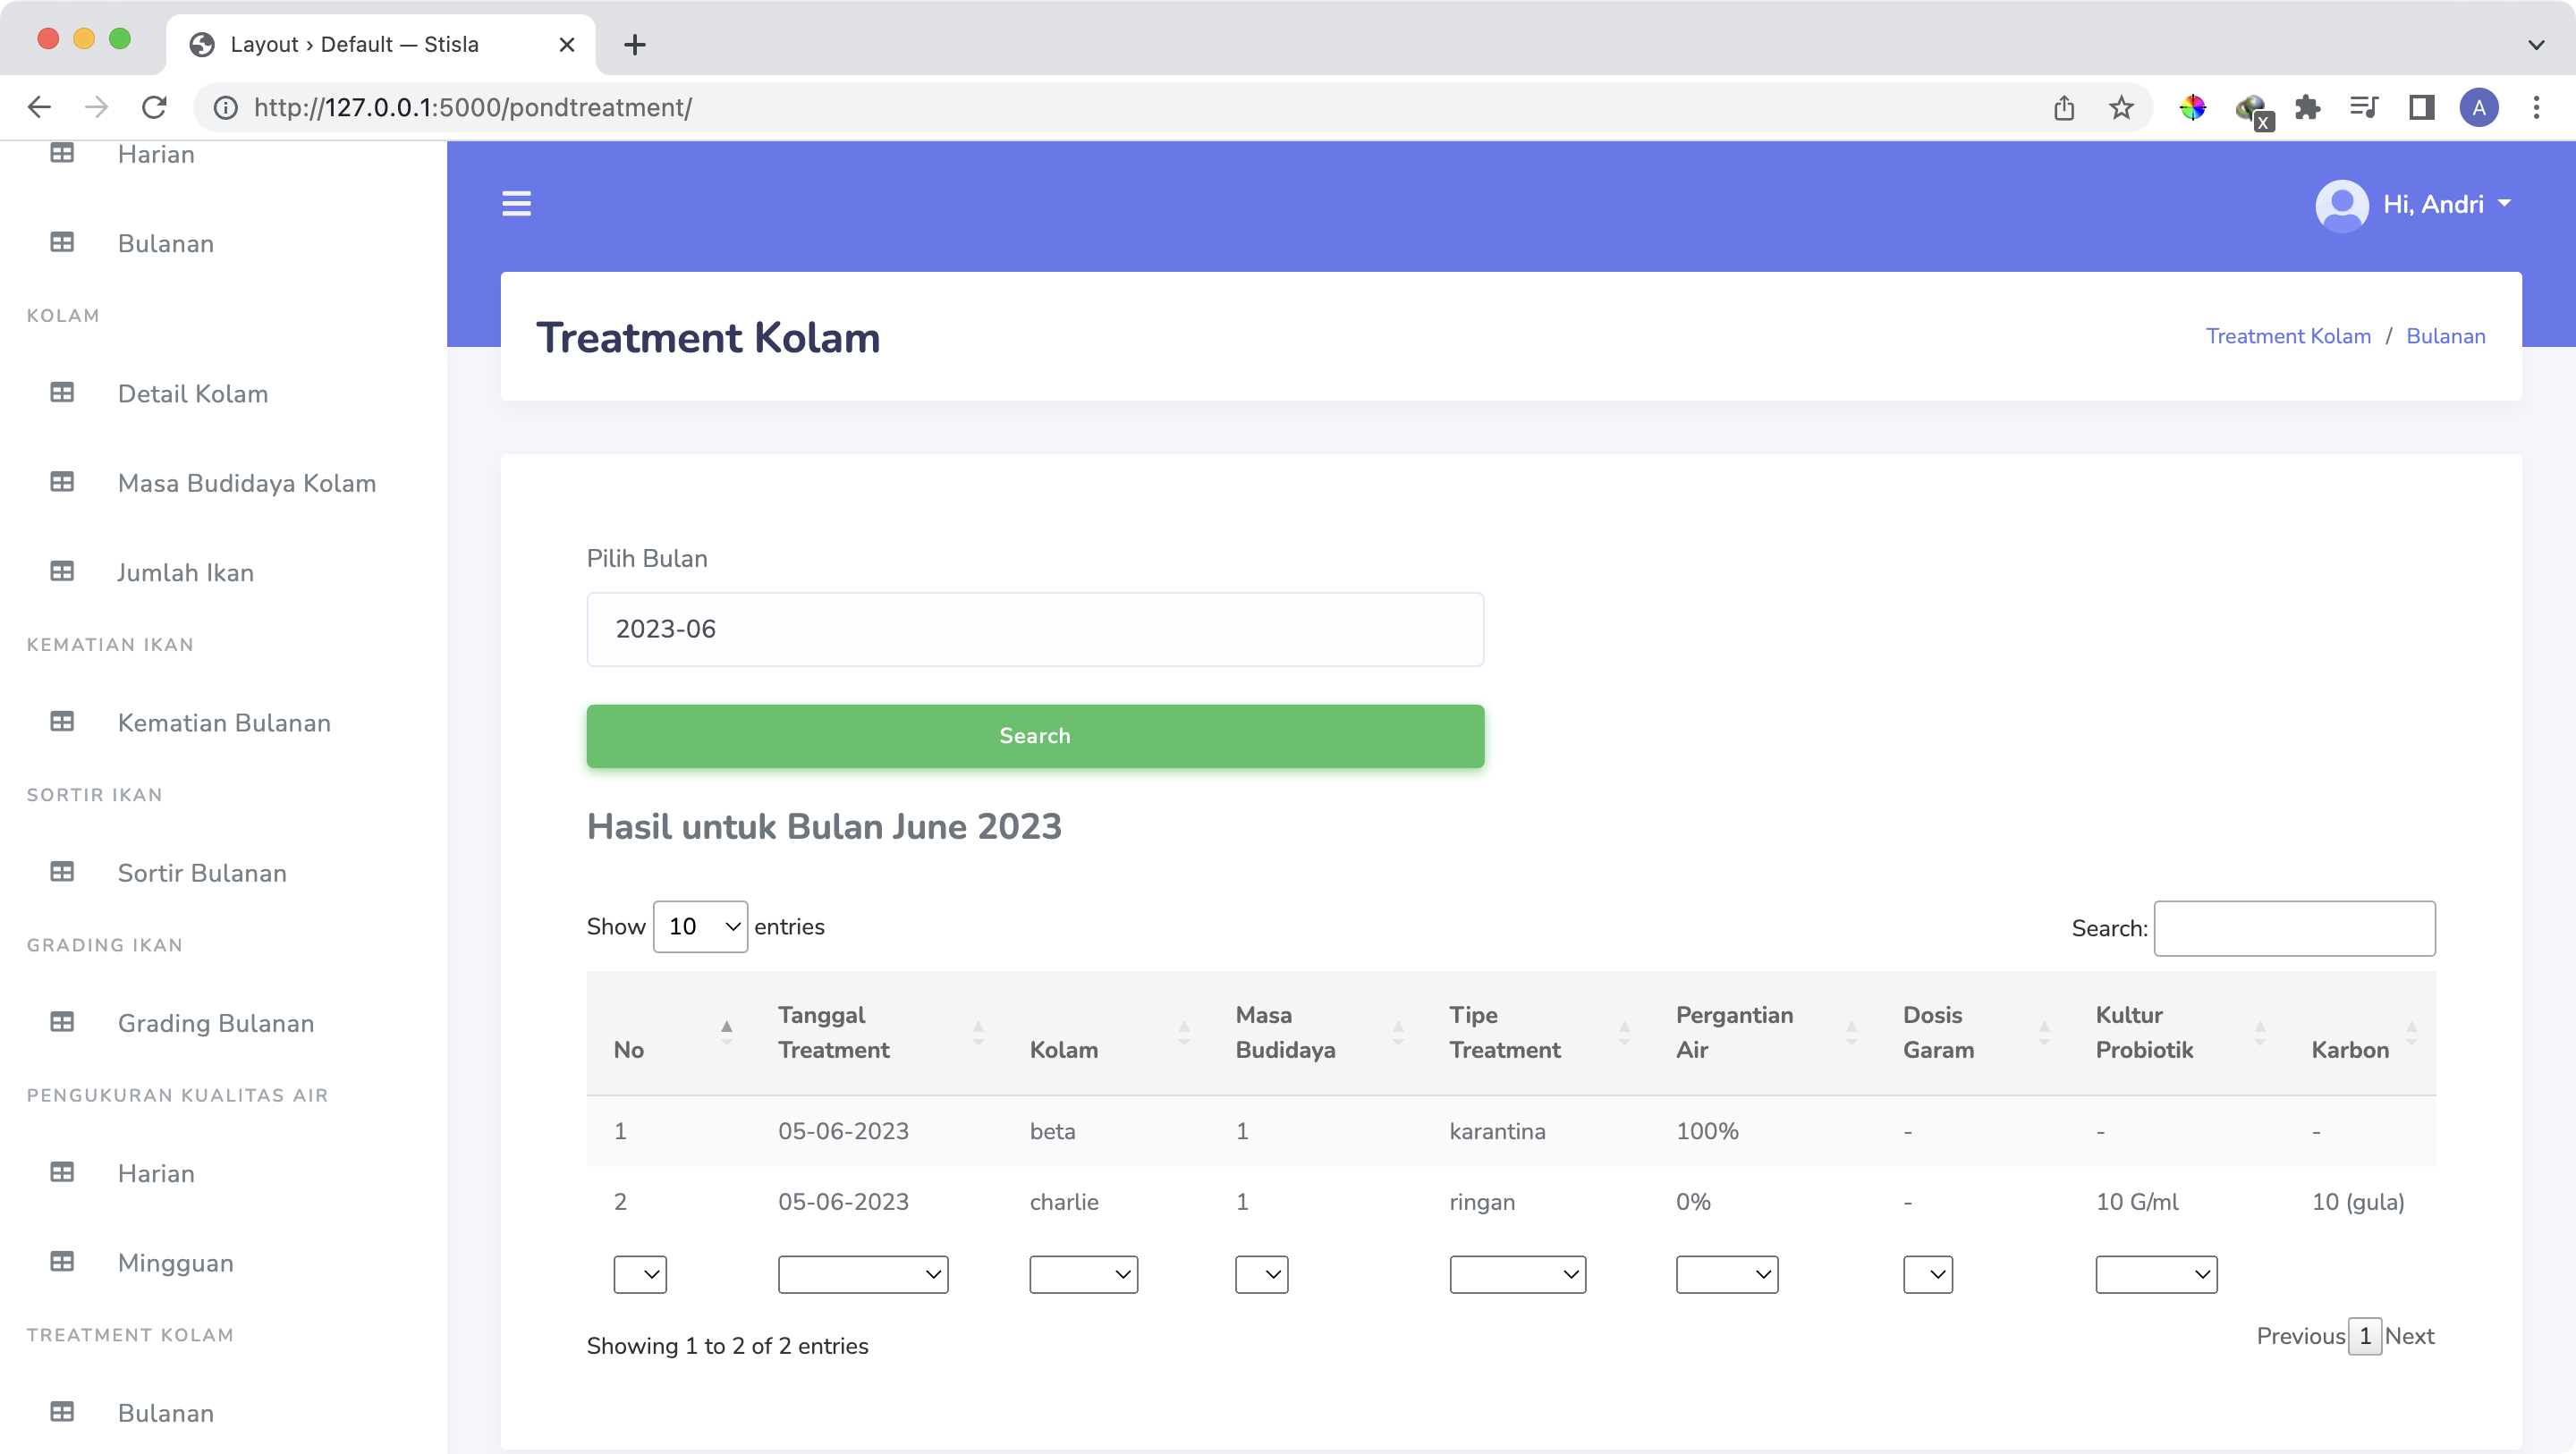
\includegraphics[width=1\textwidth]{gambar/Sprint10/view/view_rekap_treatment_kolam}
	\caption{View list pencatatan kolam harian}
	\label{fig:view_list_pencatatan_kolam_harian}
\end{figure}

\item \textbf{Membuat view rekap pencatatan kolam mingguan}
\begin{figure}[H]
	\centering
	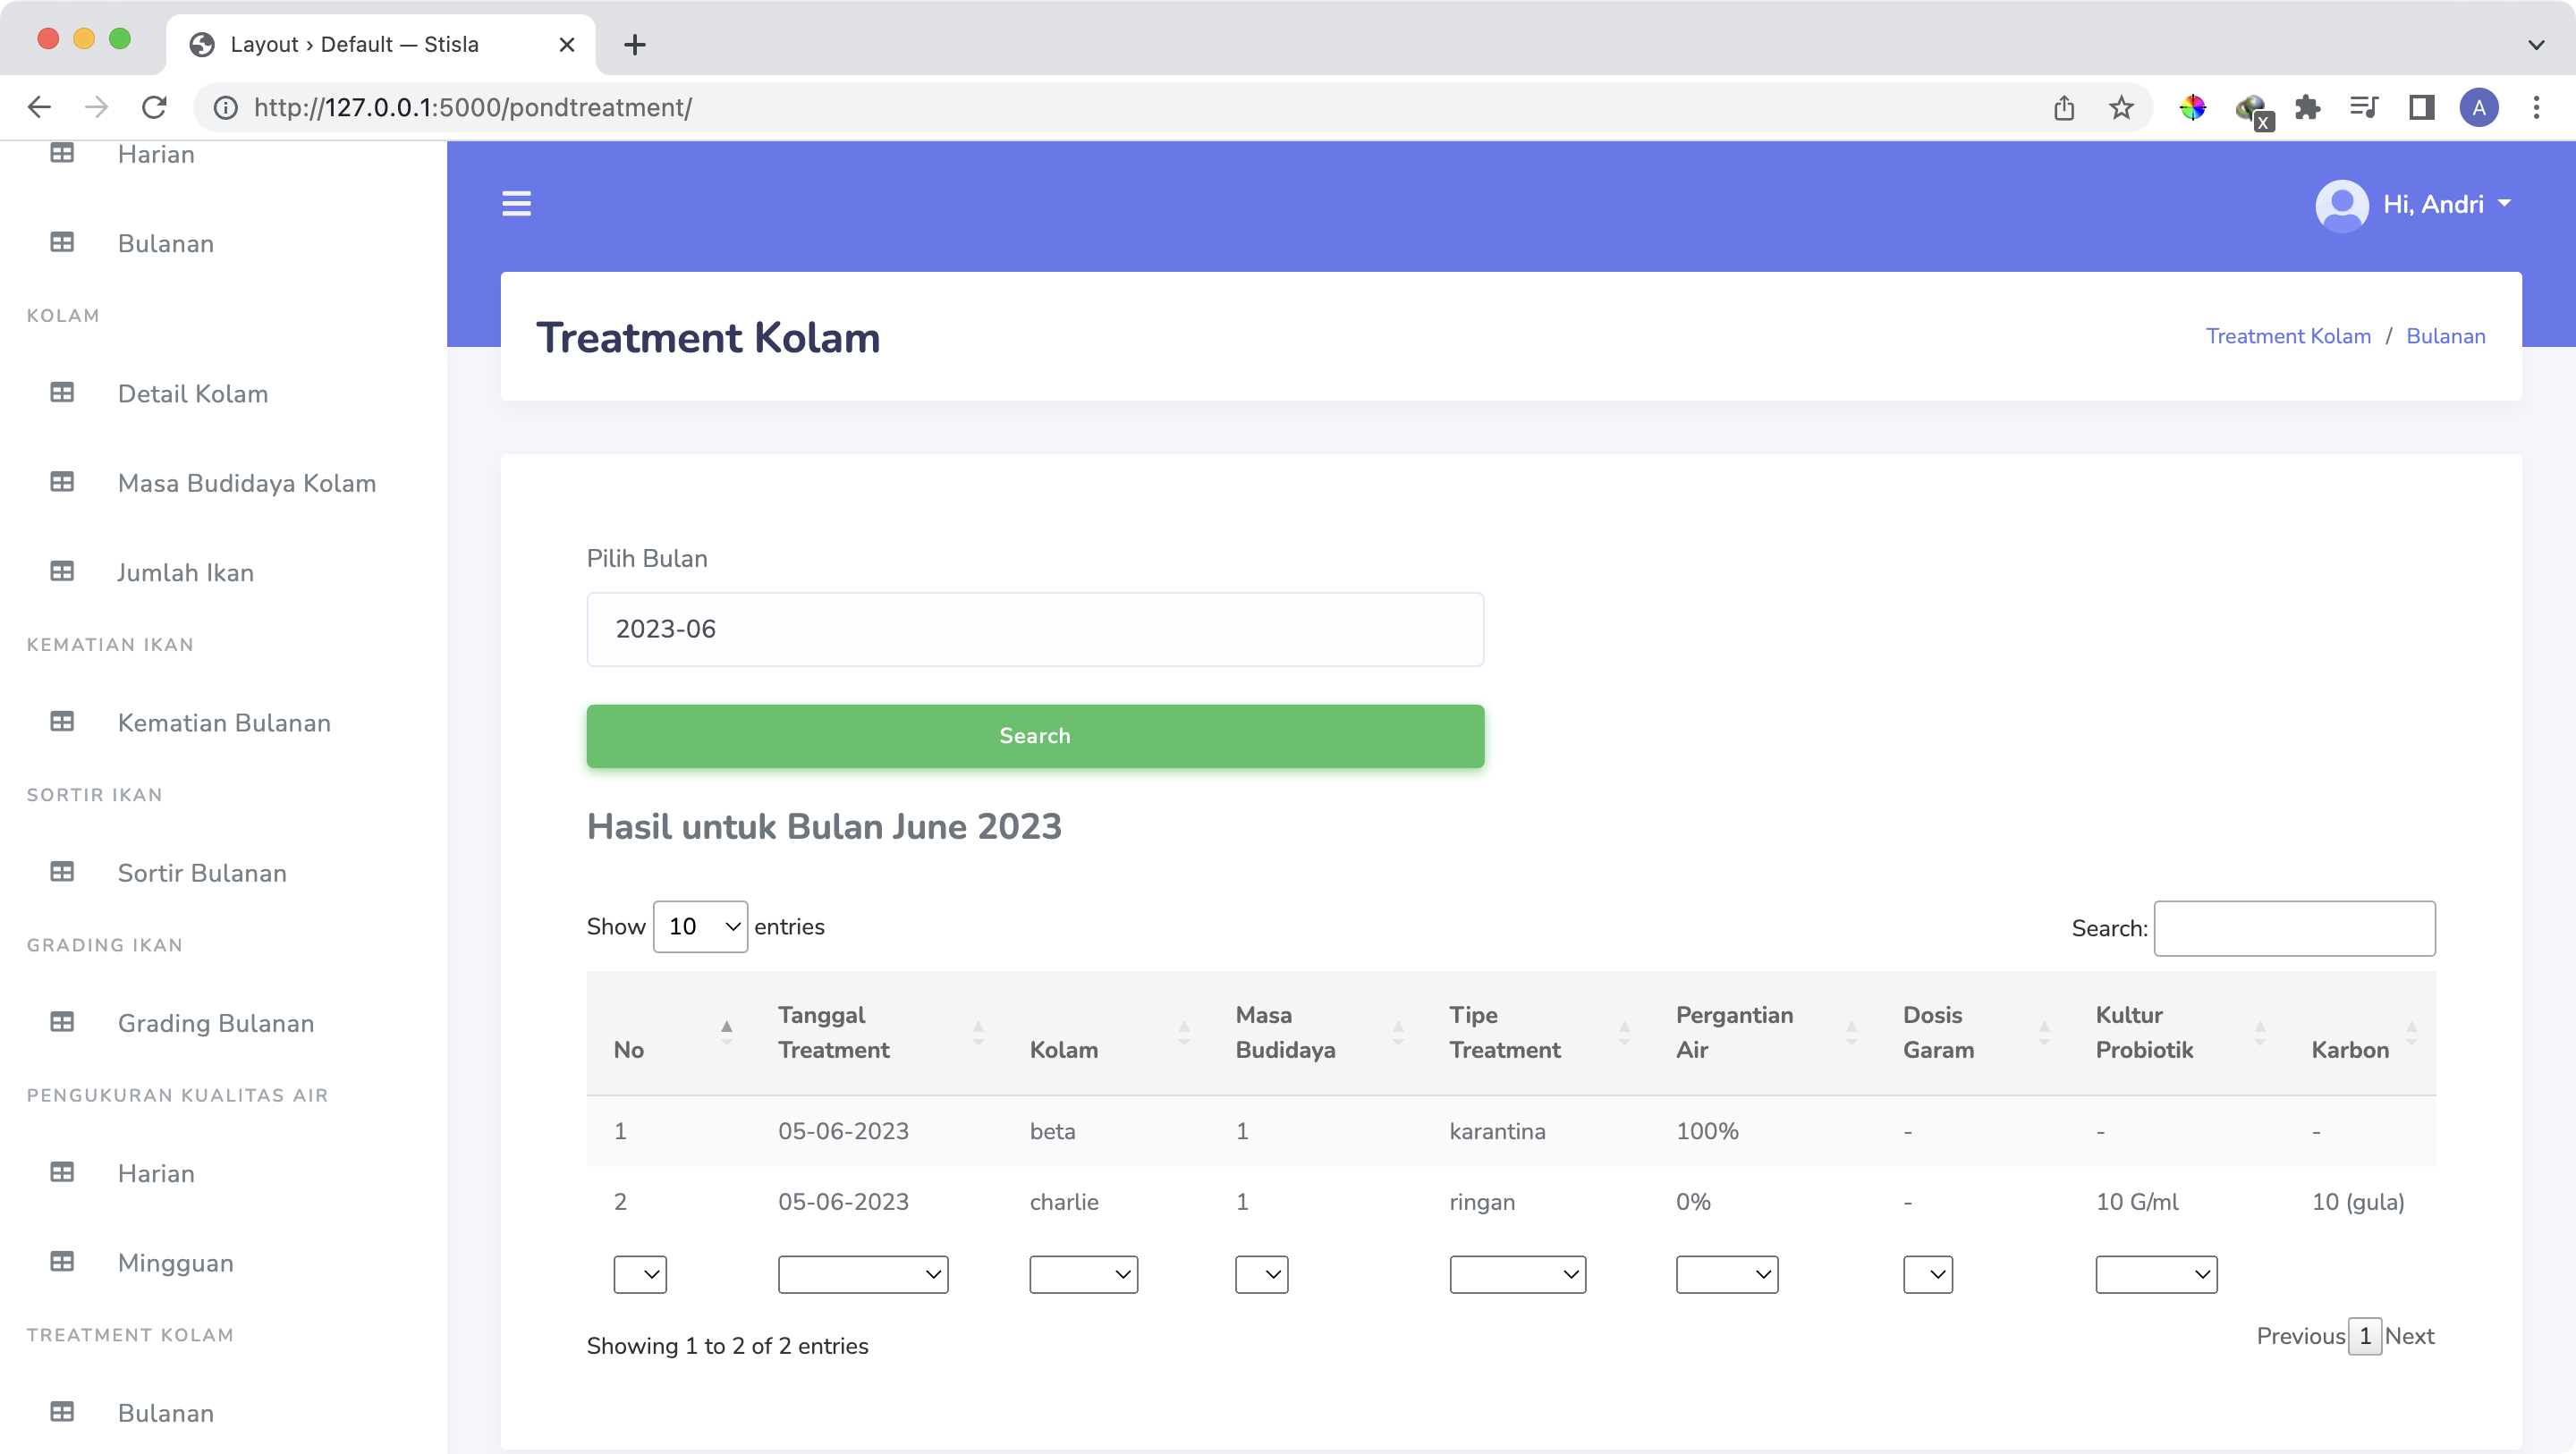
\includegraphics[width=1\textwidth]{gambar/Sprint10/view/view_rekap_treatment_kolam}
	\caption{View list pencatatan kolam mingguan}
	\label{fig:view_list_pencatatan_kolam_mingguan}
\end{figure}




\end{enumerate}
%!TEX root = ./template-skripsi.tex

\subsection{Sprint 10 Report}
Berikut merupakan report dari sprint ke-10 yang dilakukan pada tanggal 20 juli - 26 juli 2022.

\begin{table}[H]
	\caption{\textit{Sprint-10 backlog}}
	\label{sprint10_backlog}
	\begin{tabular}{@{} |p{0.5cm}|p{5cm}|p{5cm}|p{2cm}| @{}}
		\hline
		\textbf{No} & \textbf{\textit{Story}} & \textbf{\textit{Task}} & \textbf{\textit{Status}} \\
		\hline
		1 & \multirow{3}{5cm}{Create, Read, Updte, dan Delete untuk Treatment kolam} & Membarui desain database  & Completed\\
		\cline{1-1}\cline{3-4}
		2 & & Menambahkan routes API & Completed\\
		\cline{1-1}\cline{3-4}
		3 & & Implementasi controller entry treatment kolam & Completed\\
		\cline{1-1}\cline{3-4}
		4 & & Implementasi controller fetch list treatment kolam & Completed\\
		\cline{1-1}\cline{3-4}
		5 & & Implementasi controller edit treatment kolam & Completed\\
		\cline{1-1}\cline{3-4}
		6 & & Implementasi controller delete treatment kolam & Completed\\
		\cline{1-1}\cline{3-4}
		7 & & Implementasi controller fetch detail treatment kolam dengan id& Completed\\
		\cline{1-1}\cline{3-4}
		8 & & Membuat view rekap treatment kolam & Completed\\
		\cline{1-1}\cline{3-4}
		\hline
	\end{tabular}
\end{table}

\begin{enumerate}[1.]

\item \textbf{Membarui desain database}

\begin{figure}[H]
	\centering
	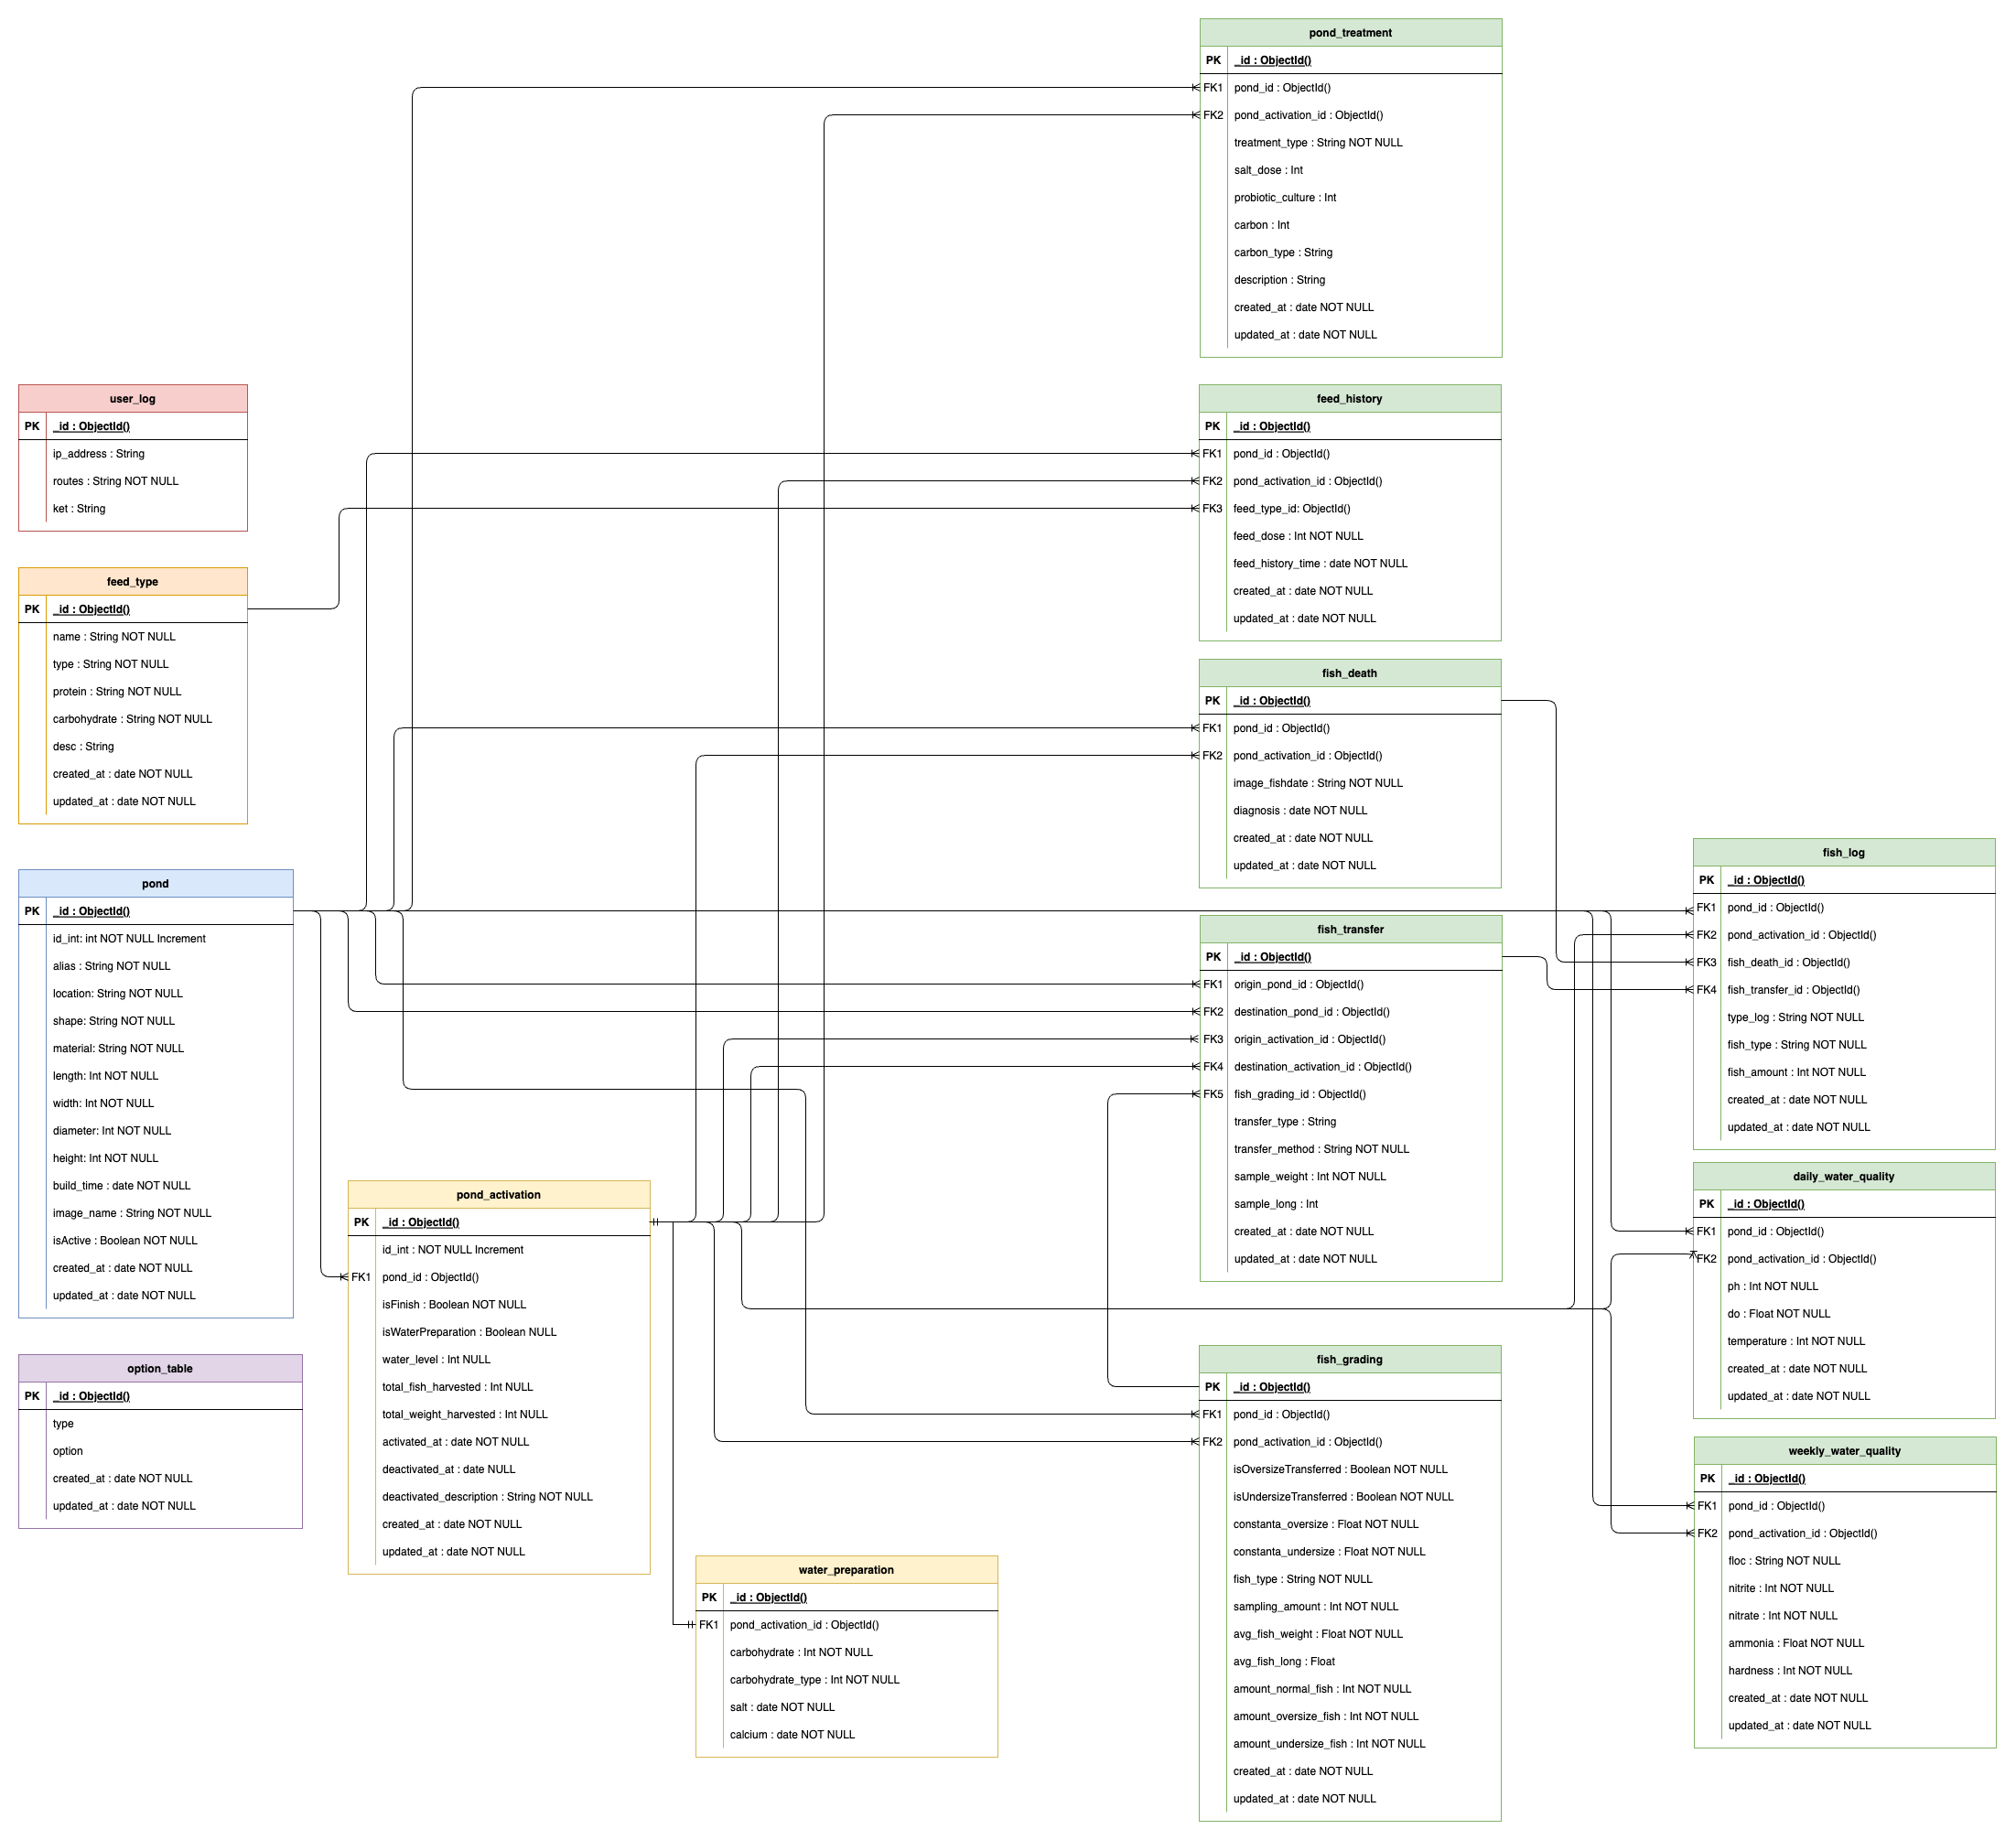
\includegraphics[height=0.7\textwidth]{gambar/Sprint10/diagram database/database}
	\caption{ERD Database Sprint-10}
	\label{fig:database_sprint10}
\end{figure}

Dengan berubahnya desain database diperlukan juga penambahan model pada source code, berikut perubahan pada source code model.

\begin{lstlisting}
# fishapi/database/model.py

class PondTreatment(db.Document):
    treatment_type_option = ("ringan", "karantina", "pergantian air")
    carbohydrate_type_option = ("", "gula", "molase", "terigu", "tapioka")

    pond_id = db.ReferenceField(Pond, required=True)
    pond_activation_id = db.ReferenceField(PondActivation, required=True)
    treatment_type = db.StringField(required=True, choices=treatment_type_option)
    water_change = db.IntField()
    salt = db.IntField()
    probiotic_culture = db.IntField()
    carbohydrate = db.IntField()
    carbohydrate_type = db.StringField(required=True, choices=carbohydrate_type_option, default="")
    description = db.StringField(default="")
    created_at = db.DateTimeField(default=datetime.datetime.now)
    updated_at = db.DateTimeField(default=datetime.datetime.now)
\end{lstlisting}



\item \textbf{Menambahkan routes API}

\begin{lstlisting}
# fishapi/resource/routes.py

# pond treatment
    api.add_resource(PondTreatmentsApi, '/api/pondtreatment')
    api.add_resource(PondTreatmentApi, '/api/pondtreatment/<id>')
\end{lstlisting}




\item \textbf{Implementasi controller entry treatment kolam}

Implementasi controller API entry treatment kolam, berikut merupakan perubahan source code controller API entry treatment kolam.

\begin{lstlisting}
# fishapi/resource/pondtreatment.py

class PondTreatmentsApi(Resource):
    def post(self):
        try:
            pond_id = request.form.get("pond_id", None)
            pond = Pond.objects.get(id=pond_id)
            if pond['isActive'] == False:
                response = {"message": "pond is not active"}
                response = json.dumps(response, default=str)
                return Response(response, mimetype="application/json", status=400)
            pond_activation = PondActivation.objects(
                pond_id=pond_id, isFinish=False).order_by('-activated_at').first()
            treatment_type = request.form.get("treatment_type", None)
            if treatment_type == "karantina":
                body = {
                    "pond_id": pond_id,
                    "pond_activation_id": pond_activation.id,
                    "treatment_type": treatment_type,
                    "water_change": 100,
                    "description": request.form.get("description", None),
                }
                pondtreatment = PondTreatment(**body).save()
                id = pondtreatment.id
                # update activation and pond
                pond_deactivation_data = {
                    "isFinish": True,
                    "total_fish_harvested": request.form.get("total_fish_harvested", None),
                    "total_weight_harvested": request.form.get("total_weight_harvested", None),
                    "deactivated_at": request.form.get("deactivated_at", datetime.datetime.now()),
                    "deactivated_description": "karantina total"
                }
                pond_activation = PondActivation.objects(
                    pond_id=pond_id, isFinish=False).order_by('-activated_at').first()
                pond_activation.update(**pond_deactivation_data)
                pond.update(**{"isActive": False})
            elif treatment_type == "ringan":
                body = {
                    "pond_id": pond_id,
                    "pond_activation_id": pond_activation.id,
                    "treatment_type": treatment_type,
                    "water_change": 0,
                    "salt": request.form.get("salt_dose", None),
                    "probiotic_culture": request.form.get("probiotic_culture", None),
                    "carbohydrate": request.form.get("carbohydrate", None),
                    "carbohydrate_type": request.form.get("carbohydrate_type", None),
                }
                pondtreatment = PondTreatment(**body).save()
                id = pondtreatment.id
            elif treatment_type == "pergantian air":
                body = {
                    "pond_id": pond_id,
                    "pond_activation_id": pond_activation.id,
                    "treatment_type": treatment_type,
                    "water_change": request.form.get("water_change", 0)
                }
                pondtreatment = PondTreatment(**body).save()
                id = pondtreatment.id
            else:
                response = {
                    "message": "treatment type just allow ['ringan','berat']"}
                response = json.dumps(response, default=str)
                return Response(response, mimetype="application/json", status=400)
            response = {
                "message": "success add data pond treatment", "id": id}
            response = json.dumps(response, default=str)
            return Response(response, mimetype="application/json", status=200)
        except Exception as e:
            response = {"message": str(e)}
            response = json.dumps(response, default=str)
            return Response(response, mimetype="application/json", status=400)
\end{lstlisting}

Kode di atas adalah implementasi sebuah API untuk menangani permintaan POST pada endpoint PondTreatmentsApi.

Pertama, kode tersebut mengambil nilai pond\_id dari formulir permintaan menggunakan request.form.get("pond\_id", None). Kemudian, dilakukan pencarian objek Pond berdasarkan pond\_id yang diperoleh.

Selanjutnya, dilakukan pengecekan apakah kolom isActive pada objek Pond memiliki nilai False. Jika iya, maka dikembalikan respons dengan pesan "pond is not active" dan status kode 400.

Selanjutnya, dilakukan pencarian objek PondActivation berdasarkan pond\_id dan isFinish=False dengan pengurutan berdasarkan activated\_at secara menurun menggunakan .order\_by('-activated\_at').first(). Nilai treatment\_type juga diambil dari formulir permintaan.

Kemudian, dilakukan pengecekan terhadap treatment\_type. Jika nilainya adalah "karantina", maka dibentuk sebuah body yang berisi data-data untuk membuat objek PondTreatment dengan beberapa nilai yang diambil dari formulir permintaan. Objek PondTreatment tersebut kemudian disimpan ke database menggunakan .save(). Nilai id dari objek tersebut diambil untuk digunakan sebagai respons.

Selanjutnya, dilakukan pembaruan (update) pada objek PondActivation dan Pond. Data-data yang diperbarui disimpan dalam variabel pond\_deactivation\_data dan pond\_activation yang merupakan objek PondActivation terakhir yang ditemukan. Objek-objek tersebut diupdate menggunakan .update().

Jika treatment\_type adalah "ringan", maka langkah yang serupa dilakukan untuk membentuk objek PondTreatment dengan data yang sesuai.

Jika treatment\_type adalah "pergantian air", maka juga dilakukan langkah yang serupa untuk membentuk objek PondTreatment dengan data yang sesuai.

Jika treatment\_type tidak sesuai dengan ketiga opsi yang diberikan ("karantina", "ringan", "pergantian air"), maka dikembalikan respons dengan pesan "treatment type just allow ['ringan','berat']" dan status kode 400.

Terakhir, jika tidak terjadi kesalahan, respons berhasil dibentuk dengan pesan "success add data pond treatment" dan nilai id dari objek PondTreatment yang telah dibuat. Respons tersebut dikonversi menjadi JSON dan dikembalikan dengan tipe konten "application/json" dan status kode 200. Jika terjadi kesalahan, tangkapan Exception akan menghasilkan pesan kesalahan yang dikirim sebagai respons dengan status kode 400.

Berikut merupakan form untuk entry grading berat ikan antar kolam.

\begin{longtable}{| l | p{5cm} | p{5cm} |}
\caption{Form entry treatment kolam.\label{table:form_entry_treatment_kolam}}\\

\hline
\multicolumn{1}{|c|}{\textbf{Form}} & \multicolumn{1}{|c|}{\textbf{Jenis Data}} & \multicolumn{1}{|c|}{\textbf{Deskripsi}}\\
\hline
\endfirsthead

\hline
\multicolumn{3}{|c|}{Lanjutan Tabel \ref{table:form_entry_treatment_kolam}}\\
\hline
\multicolumn{1}{|c|}{\textbf{Form}} & \multicolumn{1}{|c|}{\textbf{Jenis Data}} & \multicolumn{1}{|c|}{\textbf{Deskripsi}}\\
\hline
\endhead

                                          

pond\_id                 & REQUIRED STRING                                                                                          & id kolam yang akan di lakukan treatment                                      \\ \hline
treatment\_type          & REQUIRED STRING VALUE : {[}"ringan", "karantina", "pergantian air" {]}                                   & tipe treatment yang akan dilakukan                                           \\ \hline
salt                     & OPTIONAL INT                                                                                             & takaran penambahan garam ke kolam dalam satuan gram                          \\ \hline
probiotic\_culture       & OPTIONAL INT                                                                                             & takaran penambahan probiotik ke kolam dalam satuan gram                      \\ \hline
carbohydrate             & OPTIONAL INT                                                                                             & takaran penambahan zat karbon ke kolam dalam satuan gram                     \\ \hline
carbohydrate\_type       & REQUIRED IF "carbohydrate" \textgreater 0 STRING VALUE : {[}"", "gula", "molase", "terigu", "tapioka"{]} & tipe zat karbon                                                              \\ \hline
description              & OPTIONAL STRING                                                                                          & keterangan treatment kolam                                                   \\ \hline
total\_fish\_harvested   & REQUIRED IF "treatment\_type" == "karantina" INT                                                         & jumlah ikan yang di panen pada saat kolam di karantina                       \\ \hline
total\_weight\_harvested & REQUIRED IF "treatment\_type" == "karantina" INT                                                         & jumlah berat ikan yang di panen pada saat kolam di karantina dalam satuan Kg \\ \hline
water\_change            & REQUIRED IF "treatment\_type" == "pergantian air" INT                                                    & persentase pergantian air pada kolam                                         \\ \hline
\end{longtable}



Tabel di atas merupakan daftar parameter yang dapat digunakan dalam formulir permintaan (request form) pada API PondTreatmentsApi. Setiap kolom dalam tabel memiliki informasi yang relevan terkait jenis data yang diharapkan dan deskripsi dari parameter tersebut. Berikut adalah penjelasan dari setiap kolom:

\begin{enumerate}
\item pond\_id: Parameter ini harus diisi dengan tipe data STRING yang wajib ada. Parameter ini digunakan untuk mengidentifikasi kolam yang akan diberikan treatment.

\item treatment\_type: Parameter ini harus diisi dengan tipe data STRING yang wajib ada. Nilai yang dapat diterima adalah "ringan", "karantina", atau "pergantian air". Parameter ini menentukan jenis treatment yang akan dilakukan pada kolam.

\item salt: Parameter ini bersifat opsional dan harus diisi dengan tipe data INT. Parameter ini digunakan untuk menentukan takaran penambahan garam ke dalam kolam dalam satuan gram.

\item probiotic\_culture: Parameter ini bersifat opsional dan harus diisi dengan tipe data INT. Parameter ini digunakan untuk menentukan takaran penambahan probiotik ke dalam kolam dalam satuan gram.

\item carbohydrate: Parameter ini bersifat opsional dan harus diisi dengan tipe data INT. Parameter ini digunakan untuk menentukan takaran penambahan zat karbon ke dalam kolam dalam satuan gram.

\item carbohydrate\_type: Parameter ini harus diisi jika nilai dari "carbohydrate" lebih besar dari 0. Parameter ini harus diisi dengan tipe data STRING. Nilai yang dapat diterima adalah "", "gula", "molase", "terigu", atau "tapioka". Parameter ini menentukan jenis zat karbon yang ditambahkan.

\item description: Parameter ini bersifat opsional dan harus diisi dengan tipe data STRING. Parameter ini digunakan untuk memberikan keterangan tambahan mengenai treatment kolam.

\item total\_fish\_harvested: Parameter ini harus diisi jika "treatment\_type" memiliki nilai "karantina". Parameter ini harus diisi dengan tipe data INT. Parameter ini menentukan jumlah ikan yang dipanen saat kolam dalam kondisi karantina.

\item total\_weight\_harvested: Parameter ini harus diisi jika "treatment\_type" memiliki nilai "karantina". Parameter ini harus diisi dengan tipe data INT. Parameter ini menentukan jumlah berat ikan yang dipanen saat kolam dalam kondisi karantina, dalam satuan kilogram.

\item water\_change: Parameter ini harus diisi jika "treatment\_type" memiliki nilai "pergantian air". Parameter ini harus diisi dengan tipe data INT. Parameter ini menentukan persentase pergantian air pada kolam.
\end{enumerate}

Tabel ini memberikan panduan yang berguna dalam menggunakan API PondTreatmentsApi dengan benar, menunjukkan parameter apa yang harus disertakan dalam permintaan dan jenis data yang diharapkan untuk setiap parameter tersebut.


Berikut merupakan hasil test request dari API entry treatment kolam.

cURL:

\begin{lstlisting}
curl --location 'http://jft.web.id/fishapi/api/pondtreatment' \
--form 'pond_id="{pond_id}"' \
--form 'treatment_type="karantina"' \
--form 'description="penyakit ikan sekolam"'
\end{lstlisting}

response json:

\begin{lstlisting}
{
  "message": "success add data pond treatment",
  "id": "62f5248cae2842f914ee7797"
}
\end{lstlisting}




\item \textbf{Implementasi API fetch list treatment kolam}

Implementasi controller API fetch list treatment kolam, berikut merupakan source code controller API fetch list treatment kolam.

\begin{lstlisting}
# fishapi/resource/pondtreatment.py

def get(self):
        try:
            pipeline = [
                {"$sort": {"created_at": 1}},
                {'$lookup': {
                    'from': 'pond',
                    'let': {"pondid": "$pond_id"},
                    'pipeline': [
                        {'$match': {'$expr': {'$eq': ['$_id', '$$pondid']}}},
                        {"$project": {
                            "_id": 1,
                            "alias": 1,
                            "location": 1,
                            "build_at": 1,
                            "isActive": 1,
                        }}
                    ],
                    'as': 'pond'
                }},
                {'$lookup': {
                    'from': 'pond_activation',
                    'let': {"activationid": "$pond_activation_id"},
                    'pipeline': [
                        {'$match': {
                            '$expr': {'$eq': ['$_id', '$$activationid']}}},
                        {"$project": {
                            "_id": 1,
                            "isFinish": 1,
                            "isWaterPreparation": 1,
                            "water_level": 1,
                            "activated_at": 1
                        }}
                    ],
                    'as': 'pond_activation'
                }},
                {"$addFields": {
                    "pond": {"$first": "$pond"},
                    "pond_activation": {"$first": "$pond_activation"},
                }},
                {"$project": {
                    "updated_at": 0,
                    "created_at": 0,
                }}
            ]
            pondtreatment = PondTreatment.objects.aggregate(pipeline)
            list_pondtreatments = list(pondtreatment)
            response = json.dumps(list_pondtreatments, default=str)
            return Response(response, mimetype="application/json", status=200)
        except Exception as e:
            response = {"message": str(e)}
            response = json.dumps(response, default=str)
            return Response(response, mimetype="application/json", status=400)
\end{lstlisting}



Kode di atas merupakan implementasi metode get() dalam sebuah class yang mengatur API. Metode ini digunakan untuk mengambil data PondTreatment (pengobatan kolam) dari database menggunakan agregasi dengan pipeline MongoDB. Berikut adalah penjelasan langkah-langkah yang dilakukan oleh kode tersebut:

\begin{enumerate}
\item Sebuah pipeline MongoDB dibuat untuk mengatur tahapan-tahapan pemrosesan data.
\item Pada tahap pertama, data akan diurutkan berdasarkan waktu pembuatan (created\_at) secara ascending (1).
\item Tahap berikutnya adalah melakukan operasi \$lookup untuk melakukan join (penggabungan) dengan koleksi pond. Tahap ini menggabungkan data \item PondTreatment dengan data kolam yang sesuai berdasarkan pond\_id. Hasil join ini akan mencakup proyeksi hanya beberapa field yang spesifik.
\item Selanjutnya, dilakukan operasi \$lookup kedua untuk melakukan join dengan koleksi pond\_activation. Tahap ini menggabungkan data PondTreatment dengan data aktivasi kolam yang sesuai berdasarkan pond\_activation\_id. Seperti sebelumnya, hasil join ini juga mencakup proyeksi hanya beberapa field yang spesifik.
\item Setelah join, dilakukan operasi \$addFields untuk menambahkan dua field baru, yaitu pond dan pond\_activation. Nilai dari kedua field ini diambil dari elemen pertama dalam array hasil join.
\item Tahap selanjutnya adalah operasi \$project yang digunakan untuk mengatur proyeksi output, dalam hal ini menghilangkan field updated\_at dan created\_at.
\item Setelah pipeline terbentuk, pipeline ini digunakan untuk melakukan agregasi pada koleksi PondTreatment menggunakan metode aggregate(). Hasil agregasi ini akan berupa kursor MongoDB.
\item Kursor hasil agregasi diubah menjadi list dengan menggunakan fungsi list().
\item Hasil list PondTreatment yang sudah diubah ke dalam format JSON menggunakan json.dumps().
\item Hasil akhir dikembalikan sebagai respons dengan tipe Response yang memiliki tipe konten "application/json" dan status kode 200.
\item Jika terjadi exception atau kesalahan, akan di-handle dengan mengembalikan respons dengan pesan error yang sesuai dalam format JSON dan status kode 400.
\end{enumerate}
Dengan demikian, kode tersebut melakukan proses pengambilan data PondTreatment dari database menggunakan agregasi dengan pipeline, menggabungkan data dengan koleksi lain, dan mengatur format dan status respons yang dihasilkan.

Berikut merupakan hasil test request dari API fetch list treatment kolam.

cURL:

\begin{lstlisting}
curl --location 'http://jft.web.id/fishapi/api/pondtreatment'
\end{lstlisting}

response json:

\begin{lstlisting}
[
  {
    "_id": "62f5248cae2842f914ee7797",
    "pond_id": "62a62163e445ffb9c5f746f3",
    "pond_activation_id": "62d3f2180d7265ab60f9cb83",
    "treatment_type": "ringan",
    "probiotic_culture": 10,
    "carbohydrate": 10,
    "carbohydrate_type": "gula",
    "pond": {
      "_id": "62a62163e445ffb9c5f746f3",
      "alias": "charlie",
      "location": "blok 2",
      "build_at": "2022-06-13 00:24:51.473000",
      "isActive": false
    },
    "pond_activation": {
      "_id": "62d3f2180d7265ab60f9cb83",
      "isFinish": true,
      "isWaterPreparation": true,
      "water_level": 100,
      "activated_at": "2022-07-17 18:27:20.511000"
    }
  },
  {
    "_id": "62f52c34307b0c2008380309",
    "pond_id": "62a62163e445ffb9c5f746f3",
    "pond_activation_id": "62d3f2180d7265ab60f9cb83",
    "treatment_type": "karantina",
    "carbohydrate_type": "",
    "description": "penyakit ikan sekolam",
    "pond": {
      "_id": "62a62163e445ffb9c5f746f3",
      "alias": "charlie",
      "location": "blok 2",
      "build_at": "2022-06-13 00:24:51.473000",
      "isActive": false
    },
    "pond_activation": {
      "_id": "62d3f2180d7265ab60f9cb83",
      "isFinish": true,
      "isWaterPreparation": true,
      "water_level": 100,
      "activated_at": "2022-07-17 18:27:20.511000"
    }
  }
]
\end{lstlisting}



\item \textbf{Implementasi API edit treatment kolam}

Implementasi controller API edit treatment kolam, berikut merupakan perubahan source code controller API edit treatment kolam.

\begin{lstlisting}
# fishapi/database/pondtreatment.py

def put(self, id):
        try:
            body = request.form.to_dict(flat=True)
            PondTreatment.objects.get(id=id).update(**body)
            response = {
                "message": "success change data pond treatment", "id": id}
            response = json.dumps(response, default=str)
            return Response(response, mimetype="application/json", status=200)
        except Exception as e:
            response = {"message": str(e)}
            response = json.dumps(response, default=str)
            return Response(response, mimetype="application/json", status=400)
\end{lstlisting}

Kode di atas merupakan implementasi metode put() dalam sebuah modul pondtreatment.py yang berfungsi untuk memperbarui data PondTreatment (pengobatan kolam) dalam database. Berikut adalah penjelasan langkah-langkah yang dilakukan oleh kode tersebut:

\begin{enumerate}
\item Metode put() menerima parameter id yang merupakan identifikasi unik dari PondTreatment yang akan diperbarui.
\item Di dalam blok try, pertama-tama dilakukan pengambilan data dari form request menggunakan request.form.to\_dict(flat=True). Data tersebut dikonversi menjadi bentuk dictionary dengan argumen flat=True.
\item Selanjutnya, menggunakan metode get() dari PondTreatment.objects dengan memanfaatkan id yang diberikan, data PondTreatment yang sesuai diambil dari database.
\item Data PondTreatment tersebut kemudian diperbarui menggunakan metode update() dengan argumen **body, yang berarti data pada field-field yang sesuai dalam PondTreatment akan diperbarui dengan nilai baru dari body (dictionary yang berisi data dari form request).
\item Setelah proses pembaruan selesai, respons berhasil dengan pesan success dan id PondTreatment yang telah diperbarui dibuat.
\item Respons tersebut diubah menjadi format JSON menggunakan json.dumps().
\item Hasil akhir dikembalikan sebagai respons dengan tipe Response yang memiliki tipe konten "application/json" dan status kode 200.
\item Jika terjadi exception atau kesalahan, akan di-handle dengan mengembalikan respons dengan pesan error yang sesuai dalam format JSON dan status kode 400.
\end{enumerate}
Dengan demikian, kode tersebut melakukan proses pembaruan data PondTreatment dengan menggunakan data yang diterima dari form request. Data PondTreatment diambil dari database menggunakan get() dan kemudian diperbarui dengan nilai baru. Respons yang dihasilkan mengindikasikan keberhasilan pembaruan atau kesalahan yang terjadi.

Berikut merupakan hasil test request dari API edit treatment kolam.

cURL:

\begin{lstlisting}
curl --location --request PUT 'http://jft.web.id/fishapi/api/pondtreatment/62f5248cae2842f914ee7797' \
--form 'salt="20"' \
--form 'probiotic_culture="20"' \
--form 'carbohydrate="20"' \
--form 'carbohydrate_type="molase"'
\end{lstlisting}

response json:

\begin{lstlisting}
{
  "message": "success change data pond treatment",
  "id": "62f5248cae2842f914ee7797"
}
\end{lstlisting}



\item \textbf{Implementasi API delete treatment kolam}

Implementasi controller API delete treatment kolam, berikut merupakan perubahan source code controller API delete treatment kolam.

\begin{lstlisting}
# fishapi/database/pondtreatment.py

def delete(self, id):
        try:
            pondtreatment = PondTreatment.objects.get(id=id).delete()
            response = {"message": "success delete pond treatment"}
            response = json.dumps(response, default=str)
            return Response(response, mimetype="application/json", status=200)
        except Exception as e:
            response = {"message": str(e)}
            response = json.dumps(response, default=str)
            return Response(response, mimetype="application/json", status=400)
\end{lstlisting}


Kode di atas merupakan implementasi metode delete() dalam modul pondtreatment.py yang bertanggung jawab untuk menghapus data PondTreatment (pengobatan kolam) dari database. Berikut adalah penjelasan langkah-langkah yang dilakukan oleh kode tersebut:

Metode delete() menerima parameter id yang merupakan identifikasi unik dari PondTreatment yang akan dihapus. Di dalam blok try, pertama-tama dilakukan pengambilan data PondTreatment dari database menggunakan metode get() dari PondTreatment.objects dengan menggunakan id yang diberikan. Setelah data PondTreatment berhasil diambil, dilakukan penghapusan data tersebut dari database menggunakan metode delete().
Setelah proses penghapusan selesai, respons berhasil dengan pesan success dihasilkan. Respons tersebut diubah menjadi format JSON menggunakan json.dumps(). Hasil akhir dikembalikan sebagai respons dengan tipe Response yang memiliki tipe konten "application/json" dan status kode 200. Jika terjadi exception atau kesalahan, akan di-handle dengan mengembalikan respons dengan pesan error yang sesuai dalam format JSON dan status kode 400.

Dengan demikian, kode tersebut melakukan proses penghapusan data PondTreatment dari database berdasarkan id yang diberikan. Jika penghapusan berhasil, akan mengembalikan respons dengan pesan keberhasilan. Jika terjadi kesalahan, akan mengembalikan respons dengan pesan error yang sesuai.

Berikut merupakan hasil test request dari API delete treatment kolam.

cURL:

\begin{lstlisting}
curl --location --request DELETE 'http://jft.web.id/fishapi/api/pondtreatment/62e8b800ef4edacc5bb18b05'
\end{lstlisting}

response json:

\begin{lstlisting}
{
  "message": "success delete pond treatment"
}
\end{lstlisting}


\item \textbf{Implementasi API fetch detail treatment kolam dengan id}

Implementasi controller API fetch detail treatment kolam, berikut merupakan source code controller API fetch detail treatment kolam.

\begin{lstlisting}
# fishapi/resource/pondtreatment.py

def get(self, id):
        try:
            pipeline = [
                {'$match': {'$expr': {'$eq': ['$_id', {'$toObjectId': id}]}}},
                {'$lookup': {
                    'from': 'pond',
                    'let': {"pondid": "$pond_id"},
                    'pipeline': [
                        {'$match': {'$expr': {'$eq': ['$_id', '$$pondid']}}},
                        {"$project": {
                            "_id": 1,
                            "alias": 1,
                            "location": 1,
                            "build_at": 1,
                            "isActive": 1,
                        }}
                    ],
                    'as': 'pond'
                }},
                {'$lookup': {
                    'from': 'pond_activation',
                    'let': {"activationid": "$pond_activation_id"},
                    'pipeline': [
                        {'$match': {
                            '$expr': {'$eq': ['$_id', '$$activationid']}}},
                        {"$project": {
                            "_id": 1,
                            "isFinish": 1,
                            "isWaterPreparation": 1,
                            "water_level": 1,
                            "activated_at": 1
                        }}
                    ],
                    'as': 'pond_activation'
                }},
                {"$addFields": {
                    "pond": {"$first": "$pond"},
                    "pond_activation": {"$first": "$pond_activation"},
                }},
                {"$project": {
                    "updated_at": 0,
                    "created_at": 0,
                }}
            ]
            pondtreatment = PondTreatment.objects.aggregate(pipeline)
            list_pondtreatments = list(pondtreatment)
            response = json.dumps(list_pondtreatments[0], default=str)
            return Response(response, mimetype="application/json", status=200)
        except Exception as e:
            response = {"message": str(e)}
            response = json.dumps(response, default=str)
            return Response(response, mimetype="application/json", status=400)
\end{lstlisting}


Kode di atas merupakan implementasi metode get() dalam modul pondtreatment.py yang bertanggung jawab untuk mendapatkan data PondTreatment (pengobatan kolam) berdasarkan id yang diberikan dari database. Berikut adalah penjelasan langkah-langkah yang dilakukan oleh kode tersebut:

\begin{enumerate}
\item Metode get() menerima parameter id yang merupakan identifikasi unik dari PondTreatment yang ingin didapatkan.
\item Di dalam blok try, sebuah pipeline MongoDB disusun untuk melakukan agregasi data PondTreatment berdasarkan id yang diberikan.
\item Pipeline ini terdiri dari beberapa tahapan:
\begin{enumerate}
\item Pertama, dilakukan pencocokan (\$match) berdasarkan ekspresi yang membandingkan \_id dengan id yang dikonversi menggunakan \$toObjectId.
\item Selanjutnya, dilakukan operasi \$lookup untuk menggabungkan (join) dengan koleksi "pond". Hasilnya akan disimpan dalam field "pond".
\item Kemudian, dilakukan operasi \$lookup untuk menggabungkan (join) dengan koleksi "pond\_activation". Hasilnya akan disimpan dalam field "pond\_activation".
\item Selanjutnya, menggunakan \$addFields, field "pond" dan "pond\_activation" diatur sebagai nilai pertama (\$first) dari array yang dihasilkan oleh operasi \$lookup, sehingga hanya satu dokumen yang disimpan.
\item Terakhir, menggunakan \$project, field "updated\_at" dan "created\_at" dihilangkan dari hasil akhir.
\end{enumerate}
\item Setelah pipeline selesai, dilakukan agregasi data PondTreatment menggunakan PondTreatment.objects.aggregate() dengan pipeline yang telah disusun.
\item Hasil agregasi kemudian diubah menjadi list menggunakan list().
\item Dalam hal ini, dianggap bahwa hasil agregasi akan menghasilkan satu dokumen PondTreatment. Oleh karena itu, hanya elemen pertama dari list yang diambil.
\item Hasil tersebut diubah menjadi format JSON menggunakan json.dumps().
\item Hasil akhir dikembalikan sebagai respons dengan tipe Response yang memiliki tipe konten "application/json" dan status kode 200.
\item Jika terjadi exception atau kesalahan, akan di-handle dengan mengembalikan respons dengan pesan error yang sesuai dalam format JSON dan status kode 400.
\end{enumerate}

Dengan demikian, kode tersebut melakukan pengambilan data PondTreatment dari database berdasarkan id yang diberikan menggunakan operasi agregasi MongoDB. Jika pengambilan data berhasil, akan mengembalikan respons dengan data PondTreatment dalam format JSON. Jika terjadi kesalahan, akan mengembalikan respons dengan pesan error yang sesuai.


Berikut merupakan hasil test request dari API fetch treatment kolam berdasarkan id.

cURL:

\begin{lstlisting}
curl --location 'http://jft.web.id/fishapi/api/pondtreatment/62f5248cae2842f914ee7797'
\end{lstlisting}

response json:

\begin{lstlisting}
{
  "_id": "62f5248cae2842f914ee7797",
  "pond_id": "62a62163e445ffb9c5f746f3",
  "pond_activation_id": "62d3f2180d7265ab60f9cb83",
  "treatment_type": "ringan",
  "probiotic_culture": 10,
  "carbohydrate": 10,
  "carbohydrate_type": "gula",
  "pond": {
    "_id": "62a62163e445ffb9c5f746f3",
    "alias": "charlie",
    "location": "blok 2",
    "build_at": "2022-06-13 00:24:51.473000",
    "isActive": false
  },
  "pond_activation": {
    "_id": "62d3f2180d7265ab60f9cb83",
    "isFinish": true,
    "isWaterPreparation": true,
    "water_level": 100,
    "activated_at": "2022-07-17 18:27:20.511000"
  }
}
\end{lstlisting}

\item \textbf{Membuat view rekap treatment kolam}
\begin{figure}[H]
	\centering
	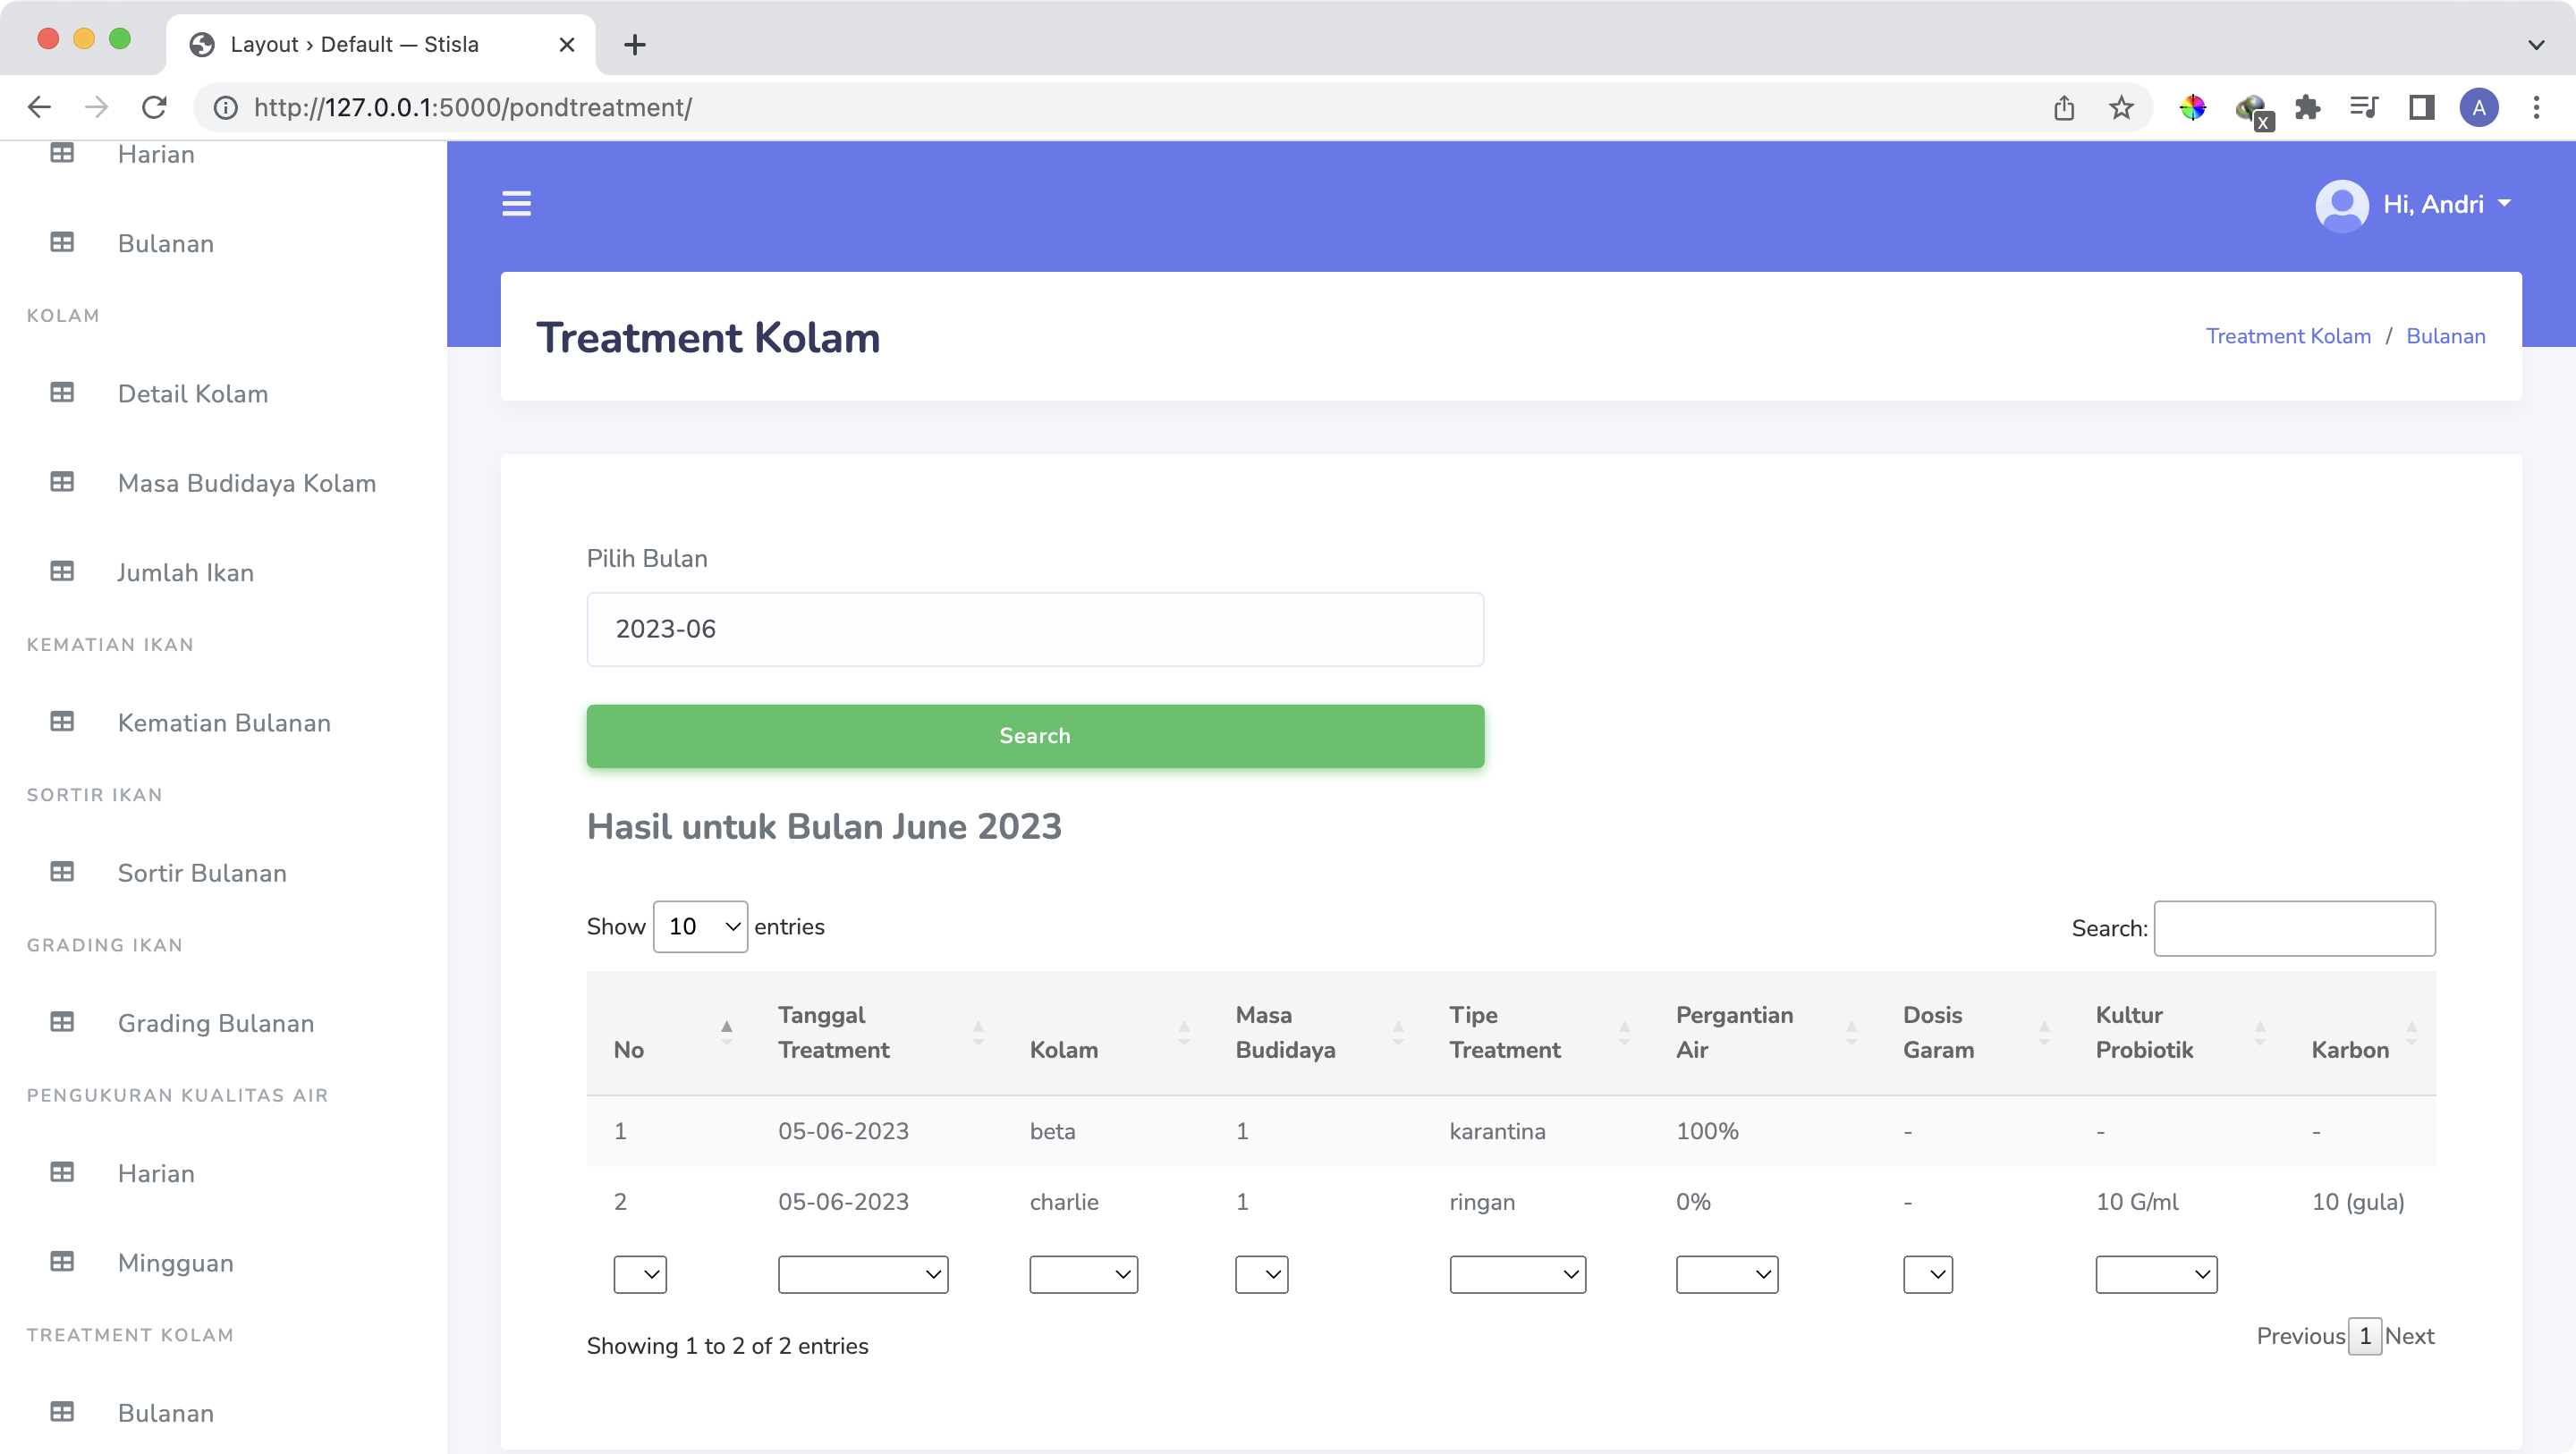
\includegraphics[width=1\textwidth]{gambar/Sprint10/view/view_rekap_treatment_kolam}
	\caption{View list treatment kolam perbulan}
	\label{fig:view_list_treatment_kolam_perbulan}
\end{figure}




\end{enumerate}
% \input{sprint11}

\section{Uji Sistem}
Pengujian sistem dilakukan menggunakan dua tipe yaitu Unit Testing dan User Acceptance Test (UAT). Pengujian dilaksanakan pada saat seluruh User Story pada Product Backlog telah diimplementasikan. Unit testing aplikasi dilakukan terhadap satu frontend developer, sedangkan pengujian User Acceptance Test dilakukan terhadap satu scrum master dan owner.

\subsection {Unit Testing}

Unit testing yang dilakukan oleh penulis dilaksanakan setiap sebelum sprint berakhir. Adapun hasil dari unit testing yang telah dilaksanakan dapat dilihat pada tabel di bawah ini:

% Pemberikan Pakan
\begin{longtable}{| p{8cm} | c | c | l |}
\caption{Unit testing fitur pemberian pakan.\label{table:unit_testing_fitur_pemberian_pakan}}\\
\hline
\multicolumn{4}{| c |}{Awal Tabel}\\
\hline
\multirow{2}{*}{Skenario Pengujian} & \multicolumn{2}{l|}{Kesesuaian}            & \multirow{2}{*}{Kesimpulan} \\ \cline{2-3}
                                    & \multicolumn{1}{l|}{sesuai} & tidak sesuai &                             \\ \hline
\hline
\endfirsthead
\hline
\multicolumn{4}{|c|}{Lanjutan \textbf{Tabel \ref{table:unit_testing_fitur_pemberian_pakan}}}\\
\hline
\multirow{2}{*}{Skenario Pengujian} & \multicolumn{2}{l|}{Kesesuaian}            & \multirow{2}{*}{Kesimpulan} \\ \cline{2-3}
                                    & \multicolumn{1}{l|}{sesuai} & tidak sesuai &                             \\ \hline
\hline
\endhead
\hline
\endfoot
\hline
\multicolumn{4}{|c|}{Akhir \textbf{Tabel \ref{table:unit_testing_fitur_pemberian_pakan}}}\\
\hline\hline
\endlastfoot
API pencatatan pemberian pakan& \Checkmark &  & Diterima                                                  \\ \hline
API merubah data pemberian pakan& \Checkmark & & Diterima                                             \\ \hline
API mendapatkan list data pemberian pakan pada suatu kolam& \Checkmark & & Diterima                                    \\ \hline
API mendapatkan detail data pemberian pakan& \Checkmark & & Diterima                                    \\ \hline
API hapus data pemeberian pakan& \Checkmark & & Diterima                                                \\ \hline
\end{longtable}


% Registrasi Kolam
\begin{longtable}{| p{8cm} | c | c | l |}
\caption{Unit testing fitur registrasi kolam.\label{table:unit_testing_fitur_registrasi_kolam}}\\
\hline
\multicolumn{4}{| c |}{Awal Tabel}\\
\hline
\multirow{2}{*}{Skenario Pengujian} & \multicolumn{2}{l|}{Kesesuaian}            & \multirow{2}{*}{Kesimpulan} \\ \cline{2-3}
                                    & \multicolumn{1}{l|}{sesuai} & tidak sesuai &                             \\ \hline
\hline
\endfirsthead
\hline
\multicolumn{4}{|c|}{Lanjutan \textbf{Tabel \ref{table:unit_testing_fitur_registrasi_kolam}}}\\
\hline
\multirow{2}{*}{Skenario Pengujian} & \multicolumn{2}{l|}{Kesesuaian}            & \multirow{2}{*}{Kesimpulan} \\ \cline{2-3}
                                    & \multicolumn{1}{l|}{sesuai} & tidak sesuai &                             \\ \hline
\hline
\endhead
\hline
\endfoot
\hline
\multicolumn{4}{|c|}{Akhir \textbf{Tabel \ref{table:unit_testing_fitur_registrasi_kolam}}}\\
\hline\hline
\endlastfoot
API pencatatan registasi kolam&\Checkmark &&Diterima\\ \hline
API merubah data kolam&\Checkmark &&Diterima\\ \hline
API mendapatkan list data kolam&\Checkmark &&Diterima\\ \hline
API mendapatkan detail data kolam&\Checkmark &&Diterima\\ \hline
API hapus data kolam&\Checkmark &&Diterima\\ \hline
\end{longtable}

% Musim budidaya Kolam
\begin{longtable}{| p{8cm} | c | c | l |}
\caption{Unit testing fitur musim budidaya kolam.\label{table:unit_testing_fitur_musim_budidaya_kolam}}\\
\hline
\multicolumn{4}{| c |}{Awal Tabel}\\
\hline
\multirow{2}{*}{Skenario Pengujian} & \multicolumn{2}{l|}{Kesesuaian}            & \multirow{2}{*}{Kesimpulan} \\ \cline{2-3}
                                    & \multicolumn{1}{l|}{sesuai} & tidak sesuai &                             \\ \hline
\hline
\endfirsthead
\hline
\multicolumn{4}{|c|}{Lanjutan \textbf{Tabel \ref{table:unit_testing_fitur_musim_budidaya_kolam}}}\\
\hline
\multirow{2}{*}{Skenario Pengujian} & \multicolumn{2}{l|}{Kesesuaian}            & \multirow{2}{*}{Kesimpulan} \\ \cline{2-3}
                                    & \multicolumn{1}{l|}{sesuai} & tidak sesuai &                             \\ \hline
\hline
\endhead
\hline
\endfoot
\hline
\multicolumn{4}{|c|}{Akhir \textbf{Tabel \ref{table:unit_testing_fitur_musim_budidaya_kolam}}}\\
\hline\hline
\endlastfoot
API memulai musim budidaya pada kolam&\Checkmark &&Diterima\\ \hline
API mengakhiri musim budidaya atau panen pada kolam&\Checkmark &&Diterima\\ \hline
API mendapatkan list status kolam&\Checkmark &&Diterima\\ \hline
API mendapatkan list musim budidaya pada suatu kolam&\Checkmark &&Diterima\\ \hline
\end{longtable}

% Kematian Ikan
\begin{longtable}{| p{8cm} | c | c | l |}
\caption{Unit testing fitur kematian ikan.\label{table:unit_testing_fitur_kematian_ikan}}\\
\hline
\multicolumn{4}{| c |}{Awal Tabel}\\
\hline
\multirow{2}{*}{Skenario Pengujian} & \multicolumn{2}{l|}{Kesesuaian}            & \multirow{2}{*}{Kesimpulan} \\ \cline{2-3}
                                    & \multicolumn{1}{l|}{sesuai} & tidak sesuai &                             \\ \hline
\hline
\endfirsthead
\hline
\multicolumn{4}{|c|}{Lanjutan \textbf{Tabel \ref{table:unit_testing_fitur_kematian_ikan}}}\\
\hline
\multirow{2}{*}{Skenario Pengujian} & \multicolumn{2}{l|}{Kesesuaian}            & \multirow{2}{*}{Kesimpulan} \\ \cline{2-3}
                                    & \multicolumn{1}{l|}{sesuai} & tidak sesuai &                             \\ \hline
\hline
\endhead
\hline
\endfoot
\hline
\multicolumn{4}{|c|}{Akhir \textbf{Tabel \ref{table:unit_testing_fitur_kematian_ikan}}}\\
\hline\hline
\endlastfoot
API pencatatan kematian ikan&\Checkmark &&Diterima\\ \hline
API merubah data kematian ikan&\Checkmark &&Diterima\\ \hline
API mendapatkan list data kematian ikan pada suatu musim budidaya&\Checkmark &&Diterima\\ \hline
API mendapatkan detail kematian ikan&\Checkmark &&Diterima\\ \hline
API hapus kematian ikan&\Checkmark &&Diterima\\ \hline
\end{longtable}

% Perpindahan Ikan antar kolam
\begin{longtable}{| p{8cm} | c | c | l |}
\caption{Unit testing fitur perpindahan ikan antar kolam.\label{table:unit_testing_fitur_perpindahan_ikan_antar_kolam}}\\
\hline
\multicolumn{4}{| c |}{Awal Tabel}\\
\hline
\multirow{2}{*}{Skenario Pengujian} & \multicolumn{2}{l|}{Kesesuaian}            & \multirow{2}{*}{Kesimpulan} \\ \cline{2-3}
                                    & \multicolumn{1}{l|}{sesuai} & tidak sesuai &                             \\ \hline
\hline
\endfirsthead
\hline
\multicolumn{4}{|c|}{Lanjutan \textbf{Tabel \ref{table:unit_testing_fitur_perpindahan_ikan_antar_kolam}}}\\
\hline
\multirow{2}{*}{Skenario Pengujian} & \multicolumn{2}{l|}{Kesesuaian}            & \multirow{2}{*}{Kesimpulan} \\ \cline{2-3}
                                    & \multicolumn{1}{l|}{sesuai} & tidak sesuai &                             \\ \hline
\hline
\endhead
\hline
\endfoot
\hline
\multicolumn{4}{|c|}{Akhir \textbf{Tabel \ref{table:unit_testing_fitur_perpindahan_ikan_antar_kolam}}}\\
\hline\hline
\endlastfoot
API pencatatan perpindahan ikan antar kolam&\Checkmark &&Diterima\\ \hline
API merubah data perpindahan ikan antar kolam&\Checkmark &&Diterima\\ \hline
API mendapatkan list data perpindahan ikan pada suatu musim budidaya&\Checkmark &&Diterima\\ \hline
API mendapatkan detail perpindahan ikan&\Checkmark &&Diterima\\ \hline
API hapus data perpindahan ikan&\Checkmark &&Diterima\\ \hline
\end{longtable}

% Grading berat ikan
\begin{longtable}{| p{8cm} | c | c | l |}
\caption{Unit testing fitur grading berat ikan.\label{table:unit_testing_fitur_grading_berat_ikan}}\\
\hline
\multicolumn{4}{| c |}{Awal Tabel}\\
\hline
\multirow{2}{*}{Skenario Pengujian} & \multicolumn{2}{l|}{Kesesuaian}            & \multirow{2}{*}{Kesimpulan} \\ \cline{2-3}
                                    & \multicolumn{1}{l|}{sesuai} & tidak sesuai &                             \\ \hline
\hline
\endfirsthead
\hline
\multicolumn{4}{|c|}{Lanjutan \textbf{Tabel \ref{table:unit_testing_fitur_grading_berat_ikan}}}\\
\hline
\multirow{2}{*}{Skenario Pengujian} & \multicolumn{2}{l|}{Kesesuaian}            & \multirow{2}{*}{Kesimpulan} \\ \cline{2-3}
                                    & \multicolumn{1}{l|}{sesuai} & tidak sesuai &                             \\ \hline
\hline
\endhead
\hline
\endfoot
\hline
\multicolumn{4}{|c|}{Akhir \textbf{Tabel \ref{table:unit_testing_fitur_grading_berat_ikan}}}\\
\hline\hline
\endlastfoot
API pencatatan grading berat ikan&\Checkmark &&Diterima\\ \hline
API merubah data grading berat ikan&\Checkmark &&Diterima\\ \hline
API mendapatkan list data grading berat ikan pada suatu musim budidaya&\Checkmark &&Diterima\\ \hline
API mendapatkan detail grading berat ikan&\Checkmark &&Diterima\\ \hline
API hapus data grading berat ikan&\Checkmark &&Diterima\\ \hline
\end{longtable}

% Pencatatan kualitas air harian
\begin{longtable}{| p{8cm} | c | c | l |}
\caption{Unit testing fitur pencatatan kualitas air harian.\label{table:unit_testing_fitur_pencatatan_kualitas_air_harian}}\\
\hline
\multicolumn{4}{| c |}{Awal Tabel}\\
\hline
\multirow{2}{*}{Skenario Pengujian} & \multicolumn{2}{l|}{Kesesuaian}            & \multirow{2}{*}{Kesimpulan} \\ \cline{2-3}
                                    & \multicolumn{1}{l|}{sesuai} & tidak sesuai &                             \\ \hline
\hline
\endfirsthead
\hline
\multicolumn{4}{|c|}{Lanjutan \textbf{Tabel \ref{table:unit_testing_fitur_pencatatan_kualitas_air_harian}}}\\
\hline
\multirow{2}{*}{Skenario Pengujian} & \multicolumn{2}{l|}{Kesesuaian}            & \multirow{2}{*}{Kesimpulan} \\ \cline{2-3}
                                    & \multicolumn{1}{l|}{sesuai} & tidak sesuai &                             \\ \hline
\hline
\endhead
\hline
\endfoot
\hline
\multicolumn{4}{|c|}{Akhir \textbf{Tabel \ref{table:unit_testing_fitur_pencatatan_kualitas_air_harian}}}\\
\hline\hline
\endlastfoot
API pencatatan kualitas air harian kolam&\Checkmark &&Diterima\\ \hline
API merubah data kualitas air harian kolam&\Checkmark &&Diterima\\ \hline
API mendapatkan list data kualitas air harian kolam pada suatu musim budidaya&\Checkmark &&Diterima\\ \hline
API mendapatkan detail kualitas air harian&\Checkmark &&Diterima\\ \hline
API hapus data kualitas air harian kolam&\Checkmark &&Diterima\\ \hline
\end{longtable}

% Pencatatan kualitas air mingguan
\begin{longtable}{| p{8cm} | c | c | l |}
\caption{Unit testing fitur pencatatan kualitas air mingguan.\label{table:unit_testing_fitur_pencatatan_kualitas_air_mingguan}}\\
\hline
\multicolumn{4}{| c |}{Awal Tabel}\\
\hline
\multirow{2}{*}{Skenario Pengujian} & \multicolumn{2}{l|}{Kesesuaian}            & \multirow{2}{*}{Kesimpulan} \\ \cline{2-3}
                                    & \multicolumn{1}{l|}{sesuai} & tidak sesuai &                             \\ \hline
\hline
\endfirsthead
\hline
\multicolumn{4}{|c|}{Lanjutan \textbf{Tabel \ref{table:unit_testing_fitur_pencatatan_kualitas_air_mingguan}}}\\
\hline
\multirow{2}{*}{Skenario Pengujian} & \multicolumn{2}{l|}{Kesesuaian}            & \multirow{2}{*}{Kesimpulan} \\ \cline{2-3}
                                    & \multicolumn{1}{l|}{sesuai} & tidak sesuai &                             \\ \hline
\hline
\endhead
\hline
\endfoot
\hline
\multicolumn{4}{|c|}{Akhir \textbf{Tabel \ref{table:unit_testing_fitur_pencatatan_kualitas_air_mingguan}}}\\
\hline\hline
\endlastfoot
API pencatatan kualitas air mingguan kolam&\Checkmark &&Diterima\\ \hline
API merubah data kualitas air mingguan kolam&\Checkmark &&Diterima\\ \hline
API mendapatkan list data kualitas air mingguan kolam pada suatu musim budidaya&\Checkmark &&Diterima\\ \hline
API mendapatkan detail kualitas air mingguan&\Checkmark &&Diterima\\ \hline
API hapus data kualitas air mingguan kolam&\Checkmark &&Diterima\\ \hline
\end{longtable}

% Pencatatan treatment kolam
\begin{longtable}{| p{8cm} | c | c | l |}
\caption{Unit testing fitur pencatatan treatment.\label{table:unit_testing_fitur_pencatatan_treatment_kolam}}\\
\hline
\multicolumn{4}{| c |}{Awal Tabel}\\
\hline
\multirow{2}{*}{Skenario Pengujian} & \multicolumn{2}{l|}{Kesesuaian}            & \multirow{2}{*}{Kesimpulan} \\ \cline{2-3}
                                    & \multicolumn{1}{l|}{sesuai} & tidak sesuai &                             \\ \hline
\hline
\endfirsthead
\hline
\multicolumn{4}{|c|}{Lanjutan \textbf{Tabel \ref{table:unit_testing_fitur_pencatatan_treatment_kolam}}}\\
\hline
\multirow{2}{*}{Skenario Pengujian} & \multicolumn{2}{l|}{Kesesuaian}            & \multirow{2}{*}{Kesimpulan} \\ \cline{2-3}
                                    & \multicolumn{1}{l|}{sesuai} & tidak sesuai &                             \\ \hline
\hline
\endhead
\hline
\endfoot
\hline
\multicolumn{4}{|c|}{Akhir \textbf{Tabel \ref{table:unit_testing_fitur_pencatatan_treatment_kolam}}}\\
\hline\hline
\endlastfoot
API pencatatan treatment kolam&\Checkmark &&Diterima\\ \hline
API merubah data treatment kolam&\Checkmark &&Diterima\\ \hline
API mendapatkan list data treatment kolam pada suatu musim budidaya&\Checkmark &&Diterima\\ \hline
API mendapatkan detail treatment kolam&\Checkmark &&Diterima\\ \hline
API hapus data treatment kolam&\Checkmark &&Diterima\\ \hline
\end{longtable}

\subsection {Pengujian Web Service}
Pengujian Web Service merupakan pengujian yang dilakukan oleh frontend developer yang akan menggunakan API pada aplikasinya.
Dalam khasus ini API di gunaakan pada aplikasi Aqua Breeding yang telah sedang dikembangkan dipenelitian lain yang sedang berjalan bersama penelitian ini. Pengujian ini bersifat berkelanjutan sesuai progress penelitian aplikasi yang dilakukan.

Pengujian dilakuan secara luring dengan frontend developer pada tanggal 16 juni 2023 yang bertempat di suatu coffee shop jakarta. Pengujian berjalan lancar dengan beberapa sedikit penyesuaian pada API. Penyesuaian bersifat minor pada respon beberapa API agar data yang dikirm sesuai dengan UI \& UX aplikasi yang sudah dibuat. Berikut merupakan beberapa tampilan halaman sistem Aqua Breeding berbasis android yang telah mengimplementasikan API yang telah dibuat.

\begin{figure}[H]
	\centering
	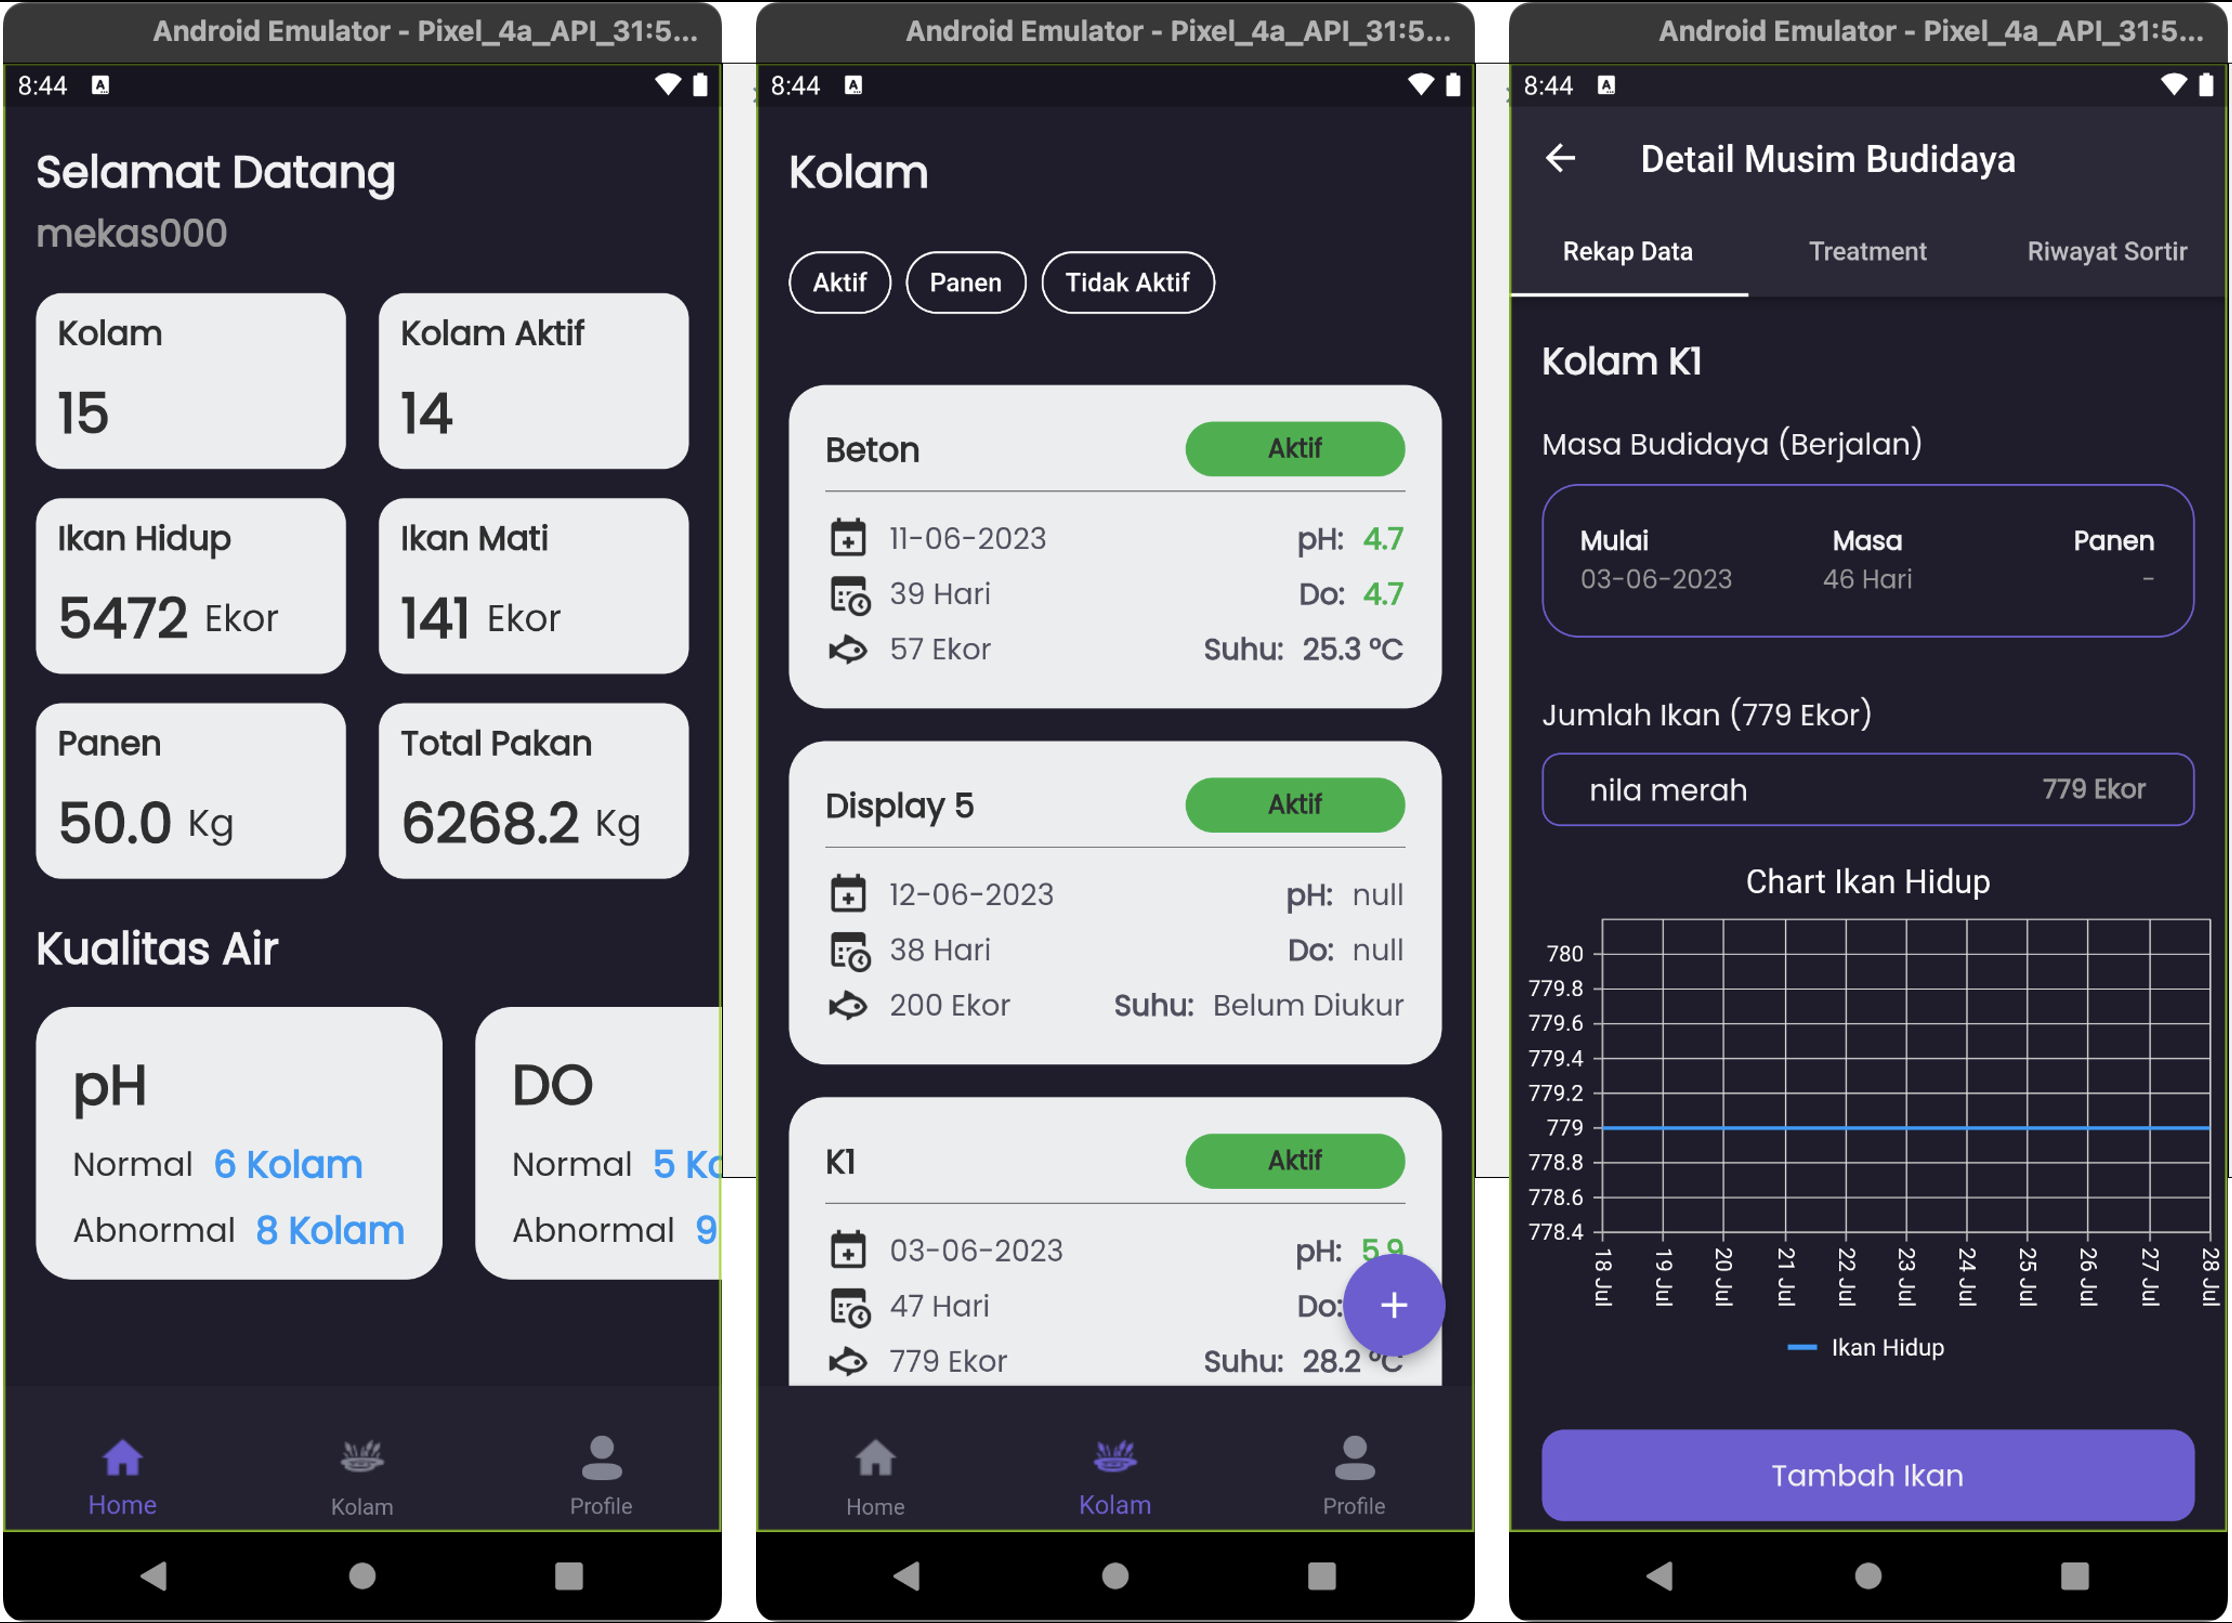
\includegraphics[width=1\textwidth]{gambar/prototipe_aqua_breeding}
	\caption{Tampilan Aqua Breeding berbasis android}
	\label{fig:aqua_breeding}
\end{figure}


\subsection {Pengujian UAT (User Acceptance Test)}
User Acceptance Test terhadap scrum master dilaksanakan pada tanggal 7 Desember 2022 secara luring bertempat di Gedung Dewi Sartika Universitas Negeri Jakarta. Adapun hasil dari UAT yang telah dilaksanakan dapat dilihat pada tabel di bawah ini:

% Pengujian UAT
\begin{longtable}{| p{8cm} | c | c | l |}
\caption{Daftar pengujian UAT.\label{table:penujian_UAT_2}}\\
\hline
\multicolumn{4}{| c |}{Awal Tabel}\\
\hline
\multirow{2}{*}{Skenario Pengujian UAT} & \multicolumn{2}{l|}{Kesesuaian}            & \multirow{2}{*}{Kesimpulan} \\ \cline{2-3}
                                    & \multicolumn{1}{l|}{sesuai} & belum &                             \\ \hline
\hline
\endfirsthead
\hline
\multicolumn{4}{|c|}{Lanjutan \textbf{Tabel \ref{table:penujian_UAT_2}}}\\
\hline
\multirow{2}{*}{Skenario Pengujian} & \multicolumn{2}{l|}{Kesesuaian}            & \multirow{2}{*}{Kesimpulan} \\ \cline{2-3}
                                    & \multicolumn{1}{l|}{sesuai} & belum &                             \\ \hline
\hline
\endhead
\hline
\endfoot
\hline
\multicolumn{4}{|c|}{Akhir \textbf{Tabel \ref{table:penujian_UAT_2}}}\\
\hline\hline
\endlastfoot
Tampilan tabel pencatatan pemberian pakan keseluruhan &&\Checkmark&Butuh Penyesuaian\\ \hline
Tampilan tabel pencatatan pemberian pakan harian &\Checkmark &&Diterima\\ \hline
Tampilan tabel pencatatan pemberian pakan bulanan &\Checkmark &&Diterima\\ \hline
Tampilan tabel kolam yang sudah di registrasi &&\Checkmark&Butuh Penyesuaian\\ \hline
Tampilan tabel masa budidaya kolam &\Checkmark &&Diterima\\ \hline
Tampilan tabel jumlah Ikan setiap  &\Checkmark &&Diterima\\ \hline
Tampilan tabel data kematian ikan&&\Checkmark &Butuh Penyesuaian\\ \hline
Tampilan tabel data sortir ikan&\Checkmark &&Diterima\\ \hline
Tampilan tabel data grading berat ikan&\Checkmark &&Diterima\\ \hline
Tampilan tabel data kualitas air harian&&\Checkmark&Butuh Penyesuaian\\ \hline
Tampilan tabel data kualitas air mingguan&&\Checkmark &Butuh Penyesuaian\\ \hline
Tampilan tabel data treatment kolam&\Checkmark &&Diterima\\ \hline
\end{longtable}

Penyesuaian pada UAT bersifat minor seperti panambahan kolom, menambahkan keterangan satuan ukur, dan rata - rata data di dalam suatu kolam. Perbaikan ini dikerjakan selama satu minggu setelah UAT. Pertemuan dilakukan lagi setelah satu minggu, yaitu pada tanggal 14 Desember 2023 untuk melaporkan perbaikan kepada scrum master.

% Baris ini digunakan untuk membantu dalam melakukan sitasi
% Karena diapit dengan comment, maka baris ini akan diabaikan
% oleh compiler LaTeX.
\begin{comment}
\bibliography{daftar-pustaka}
\end{comment}